% Canevas et spécimens de thèse.
%
%    \begin{macrocode}
%<*flat-template|these-master>
%<<COMMENT
% Document de classe yathesis
%COMMENT
\documentclass{yathesis}
%</flat-template|these-master>
%<*these-sample|flat-sample>
%<<COMMENT
% Document de classe yathesis, en 12 points, interligne un et demi, et version finale
%COMMENT
\documentclass[12pt,space=onehalf,version=final]{yathesis}
%</these-sample|flat-sample>
%<*these-sample|flat-sample|flat-template|these-master>
%<<COMMENT
%
% Chargement manuel de packages (pas déjà chargés par la classe yathesis)
%COMMENT
\usepackage[T1]{fontenc}
\usepackage[utf8]{inputenc}
%<these-sample|flat-sample>\usepackage{lipsum} % À proscrire dans un vrai mémoire de thèse !
\usepackage{kpfonts}
\usepackage{booktabs}
\usepackage{siunitx}
\usepackage{pgfplots}
\usepackage{floatrow}
\usepackage{caption}
%<these-sample|flat-sample>\usepackage{listings}
\usepackage{microtype}
\usepackage{varioref}
%<these-sample|flat-sample>\usepackage[xindy,quiet]{imakeidx}
%<these-master|flat-template>%\usepackage[xindy,quiet]{imakeidx}
%<these-sample|flat-sample>\usepackage[autostyle]{csquotes}
%<these-master|flat-template>%\usepackage[autostyle]{csquotes}
%<these-sample|flat-sample>\usepackage[backend=biber,safeinputenc]{biblatex}
%<these-master|flat-template>%\usepackage[backend=biber,safeinputenc]{biblatex}
\usepackage{hyperref}
%</these-sample|flat-sample|flat-template|these-master>
%<these-sample|flat-sample>\usepackage[xindy,acronyms,symbols]{glossaries}
%<these-master|flat-template>%\usepackage[xindy,acronyms,symbols]{glossaries}
%<*flat-template|flat-sample|these-master|these-sample>
%<<COMMENT
%
%COMMENT
%<flat-template|these-master>% (Facultatif) Génération de l'index (obligatoire si un package d'index, par
%<flat-template|these-master>% exemple « imakeidx », est chargé)
%<flat-template|these-master>% \makeindex
%<these-sample|flat-sample>% Génération de l'index
%<these-sample|flat-sample>\makeindex
%<<COMMENT
%
%COMMENT
%<flat-template|these-master>% (Facultatif) Spécification de la ou des ressources bibliographiques
%<flat-template|these-master>% (obligatoire si le package « biblatex » est chargé)
%<flat-template>% \addbibresource{}
%<flat-template>% \addbibresource{}
%<these-master>% \addbibresource{auxiliaires/bibliographie.bib}
%<these-master>% \addbibresource{auxiliaires/}
%<these-sample|flat-sample>% Spécification de la ou des ressources bibliographiques
%<flat-sample>\addbibresource{bibliographie.bib}
%<these-sample>\addbibresource{auxiliaires/bibliographie.bib}
%<these-sample|flat-sample>\addbibresource{biblatex-examples.bib} % Fournie par biblatex.
%<<COMMENT
%
%COMMENT
%<flat-template|these-master>% (Facultatif) Génération du glossaire (obligatoire si le package « glossaries »
%<flat-template|these-master>% est chargé)
%<flat-template|these-master>% \makeglossaries
%<these-sample|flat-sample>% Génération du glossaire
%<these-sample|flat-sample>\makeglossaries
%<<COMMENT
%
%COMMENT
%<flat-template|these-master>% (Facultatif) Configuration des styles du glossaire et de la liste d'acronymes
%<flat-template|these-master>% (à n'utiliser que si le package « glossaries » est chargé)
%<flat-template|these-master>% \setglossarystyle{indexhypergroup}
%<flat-template|these-master>% \setacronymstyle{long-sc-short}
%<these-sample|flat-sample>% (Facultatif) Configuration des styles du glossaire et de la liste d'acronymes
%<these-sample|flat-sample>% (à n'utiliser que si le package « glossaries » est chargé)
%<these-sample|flat-sample>\setglossarystyle{indexhypergroup}
%<these-sample|flat-sample>\setacronymstyle{long-sc-short}
%<<COMMENT
%
%COMMENT
%<flat-template|these-master|these-sample>% (Facultatif) Spécification de la ou des ressources terminologiques
%<flat-template>% \loadglsentries{}
%<flat-template>% \loadglsentries{}
%<flat-template>% \loadglsentries{}
%<these-master>% \loadglsentries{auxiliaires/}
%<these-master>% \loadglsentries{auxiliaires/}
%<these-master>% \loadglsentries{auxiliaires/}
%<these-sample>\loadglsentries{auxiliaires/glossaire}
%<these-sample>\loadglsentries{auxiliaires/acronymes}
%<these-sample>\loadglsentries{auxiliaires/symboles}
%</flat-template|flat-sample|these-master|these-sample>
%<flat-sample>% Entrées du glossaire, des acronymes et des symboles
%<flat-sample>% Glossaire
%<*flat-sample|glossary-sample>
\newglossaryentry{latex}{%
  name=\LaTeX,%
  description=système de composition de beaux documents%
}
\newglossaryentry{vrnc}{%
  name=langue vernaculaire,%
  plural=langues vernaculaires,%
  description=langue locale parlée au sein d'une communauté%
}
\newglossaryentry{af}{%
  name=ancien français,%
  description= état du français médiéval du \textsc{ix}\ieme{} au
  \textsc{xiii}\ieme{} siècles inclus%
}
\newglossaryentry{mf}{%
  name= moyen français,%
  description= état du français médiéval du \textsc{xiv}\ieme{} au \textsc{xv}\ieme{}
  siècles inclus%
}
%</flat-sample|glossary-sample>
%<flat-sample>% Acronymes
%<*flat-sample|acronyms-sample>
\newacronym{pres}{pres}{Pôle de Recherche et d'Enseignement
  Supérieur}
\newacronym{comue}{comue}{Communauté d'universités et établissements}
\newacronym{ulco}{ulco}{Université du Littoral Côte d'Opale}
\newacronym{edspi}{edspi}{École Doctorale Sciences Pour
  l'Ingénieur}
\newacronym{lmpa}{lmpa}{Laboratoire de Mathématiques Pures et
  Appliquées Joseph Liouville}
\newacronym{laser}{laser}{Light Amplification by Stimulated Emission
  of Radiation soit \enquote{amplification de la lumière par
    émission stimulée de rayonnement}}
\newacronym{irm}{irm}{Imagerie par Résonance Magnétique}
\newacronym{rmn}{rmn}{Résonance Magnétique Nucléaire}
\newacronym{ascii}{ascii}{American Standard Code for Information Interchange}
\newacronym{bios}{bios}{Basic Input Output System}
\newacronym{ctan}{ctan}{Comprehensive \TeX{} Archive Network}
\newacronym{dvd}{dvd}{Digital Video Disc}
\newacronym{erp}{erp}{Enterprise Resource Planning}
\newacronym{faq}{faq}{Frequently Asked Questions, traduit en français par
  \enquote{Foire Aux Questions}}
\newacronym{gnu}{gnu}{GNU's Not Unix (acronyme récursif)}
\newacronym{http}{http}{Hypertext Transfer Protocol}
\newacronym{ip}{ip}{Internet Protocol}
\newacronym{jpeg}{jpeg}{Joint Photographic Experts Group}
\newacronym{kdm}{kdm}{KDE Display Manager}
\newacronym{lug}{lug}{Linux Users Group}
\newacronym{mac}{mac}{Medium Access Control}
\newacronym{nfs}{nfs}{Network File System}
\newacronym{ocr}{ocr}{Optical Character Recognition}
\newacronym{p2p}{p2p}{Peer to Peer}
\newacronym{ram}{ram}{Random Access Memory}
\newacronym{radar}{radar}{RAdio Detection And Ranging}
\newacronym{svg}{svg}{Scalable Vector Graphics}
\newacronym{tft}{tft}{Thin-Film Transistor}
\newacronym{utf-8}{utf-8}{Unicode Transformation Format 8 bits}
\newacronym{vga}{vga}{Video Graphics Array}
\newacronym{wpa}{wpa}{Wi-Fi Protected Access}
\newacronym{xhtml}{xhtml}{Extensible HyperText Markup Language}
\newacronym{fsf}{fsf}{Free Software Foundation}
\newacronym{gui}{gui}{Graphical User Interface}
%</flat-sample|acronyms-sample>
%<flat-sample>% Symboles
%<*flat-sample|symbols-sample>
\newglssymbol{ohm}{\si{\ohm}}{ohm}{unité de résistance électrique}
\newglssymbol{exists}{\ensuremath{\exists}}{quantificateur existentiel}{}
\newglssymbol[constanteplanck]{planck}{\ensuremath{h}}{constante de
  Planck}{\ensuremath{h\approx\SI{6,62606957e-34}{\joule\second}}}
%</flat-sample|symbols-sample>
%<*these-sample|these-master>
%<<COMMENT
%
% Les réglages figurant habituellement dans le préambule, notamment concernant
% la bibliographie et l'éventuel index, peuvent être saisis dans le fichier
% « thesis.cfg » (situé dans le sous-dossier « configuration ») qui est
% automatiquement importé par la classe yathesis.
%COMMENT
%</these-sample|these-master>
%<*cfg-master|cfg-sample>
%<<COMMENT
%%%%%%%%%%%%%%%%%%%%%%%%%%%%%%%%%%%%%%%%%%%%%%%%%%%%%%%%%%%%%%%%%%%%%%%%%%%%%%%
% Ce fichier doit s'appeler « thesis.cfg » et se situer dans le dossier
% « configuration » ; sinon, la classe yathesis ne le détectera pas.
%%%%%%%%%%%%%%%%%%%%%%%%%%%%%%%%%%%%%%%%%%%%%%%%%%%%%%%%%%%%%%%%%%%%%%%%%%%%%%%
%COMMENT
%</cfg-master|cfg-sample>
%<*flat-template|flat-sample|cfg-master|cfg-sample>
%<*cfg-sample|flat-sample>
%<<COMMENT
%
% Configuration globale de l'apparence des listings informatiques
%COMMENT
\lstset{%
  language=C,
  numbers=left,
  frame=leftline,
  framerule=0.8pt,
  rulecolor=\color{red},
  basicstyle=\ttfamily,
  keywordstyle=\color{blue}\bfseries,
  stringstyle=\color{cyan},
  commentstyle=\color{gray}\itshape
}
%<<COMMENT
%
% Les figures flottantes et leurs légendes sont dans un (même) cadre
%COMMENT
\floatsetup[figure]{style=BOXED}%
%<<COMMENT
%
% Numéro de version du package pgfplots
%COMMENT
\pgfplotsset{compat=1.13}
%<<COMMENT
%
% Ajustement pour éviter, dans la table des matières, des débordements de
% numéros de pages dans la marge de droite
%COMMENT
\makeatletter
\renewcommand*\@pnumwidth{29pt}
\makeatother
%<<COMMENT
%COMMENT
%</cfg-sample|flat-sample>
%</flat-template|flat-sample|cfg-master|cfg-sample>
%<*flat-sample|these-sample|these-master>
%<<COMMENT
%
%COMMENT
%<these-sample|these-master>% Importation manuelle du fichier de macros personnelles
%<!flat-sample>
\def\a{A}
\def\b{B}
\def\c{C}

%</flat-sample|these-sample|these-master>
%<*macros-master>
%</macros-master>
%<*flat-sample|macros-sample>
%<<COMMENT
% Macro pour mettre en forme les noms de fichiers
%COMMENT
\newcommand{\fichier}[1]{\texttt{#1}}
%<<COMMENT
% Macro pour mettre en forme les noms de packages LaTeX
%COMMENT
\newcommand{\package}[1]{\textsf{#1}}
%<<COMMENT
% Macro pour mettre en forme des locutions étrangères
%COMMENT
\newcommand{\locution}[1]{\emph{#1}}
%</flat-sample|macros-sample>
%<*these-sample|flat-sample>
%<<COMMENT
%
% Commande permettant de faire figurer d'un seul coup toutes les références des
% ressources bibliographiques ci-dessus, même si elles ne sont pas citées
% explicitement (à proscrire dans un vrai mémoire de thèse !)
%COMMENT
\nocite{*}
%</these-sample|flat-sample>
%<*these-sample|flat-sample|flat-template|these-master>
%<<COMMENT
%
%%%%%%%%%%%%%%%%%%%%%%%%%%%%%%%%%%%%%%%%%%%%%%%%%%%%%%%%%%%%%%%%%%%%%%%%%%%%%%%
%%%%%%%%%%%%%%%%%%%%%%%%%%%%%%%%%%%%%%%%%%%%%%%%%%%%%%%%%%%%%%%%%%%%%%%%%%%%%%%
% Début du document
%%%%%%%%%%%%%%%%%%%%%%%%%%%%%%%%%%%%%%%%%%%%%%%%%%%%%%%%%%%%%%%%%%%%%%%%%%%%%%%
%%%%%%%%%%%%%%%%%%%%%%%%%%%%%%%%%%%%%%%%%%%%%%%%%%%%%%%%%%%%%%%%%%%%%%%%%%%%%%%
%COMMENT
\begin{document}
%<<COMMENT
%
%%%%%%%%%%%%%%%%%%%%%%%%%%%%%%%%%%%%%%%%%%%%%%%%%%%%%%%%%%%%%%%%%%%%%%%%%%%%%%%
% Caractéristiques du document
%%%%%%%%%%%%%%%%%%%%%%%%%%%%%%%%%%%%%%%%%%%%%%%%%%%%%%%%%%%%%%%%%%%%%%%%%%%%%%%
%
% Préparation des pages de couverture et de titre
%%%%%%%%%%%%%%%%%%%%%%%%%%%%%%%%%%%%%%%%%%%%%%%%%%%%%%%%%%%%%%%%%%%%%%%%%%%%%%%
%COMMENT
%</these-sample|flat-sample|flat-template|these-master>
%<*these-sample|these-master>
%<<COMMENT
% Les caractéristiques de la thèse sont saisies dans le fichier
% « characteristics.tex » (situé dans le dossier « configuration »).
%COMMENT
%</these-sample|these-master>
%<*flat-template|flat-sample|characteristics-sample|characteristics-master>
%<<COMMENT
% Auteur de la thèse : prénom (1er argument obligatoire), nom (2e argument
% obligatoire) et éventuel courriel (argument optionnel). Les éventuels accents
% devront figurer et le nom /ne/ doit /pas/ être saisi en capitales
%COMMENT
%<flat-template|characteristics-master>\author[]{}{}
%<characteristics-sample|flat-sample>\author[aa@zygo.fr]{Alphonse}{Allais}
%<<COMMENT
%
% Titre de la thèse dans la langue principale (argument obligatoire) et dans la
% langue secondaire (argument optionnel)
%COMMENT
%<flat-template|characteristics-master>\title[]{}
%<characteristics-sample|flat-sample>\title[Laugh's Chaos]{Le chaos du rire}
%<<COMMENT
%
% (Facultatif) Sous-titre de la thèse dans la langue principale (argument
% obligatoire) et dans la langue secondaire (argument optionnel)
%COMMENT
%<flat-template|characteristics-master>% \subtitle[]{}
%<characteristics-sample|flat-sample>\subtitle[Chaos' Laugh]{Le rire du chaos}
%<<COMMENT
%
% Champ disciplinaire dans la langue principale (argument obligatoire) et dans
% la langue secondaire (argument optionnel)
%COMMENT
%<flat-template|characteristics-master>\academicfield[]{}
%<characteristics-sample|flat-sample>\academicfield[Mathematics]{Mathématiques}
%<<COMMENT
%
% (Facultatif) Spécialité dans la langue principale (argument obligatoire) et
% dans la langue secondaire (argument optionnel)
%COMMENT
%<flat-template|characteristics-master>\speciality[]{}
%<characteristics-sample|flat-sample>\speciality[Dynamical systems]{Systèmes dynamiques}
%<<COMMENT
%
% Date de la soutenance, au format {jour}{mois}{année} donnés sous forme de
% nombres
%COMMENT
%<flat-template|characteristics-master>\date{}{}{}
%<characteristics-sample|flat-sample>\date{1}{1}{2015}
%<<COMMENT
%
% (Facultatif) Date de la soumission, au format {jour}{mois}{année} donnés sous
% forme de nombres
%COMMENT
%<flat-template|characteristics-master>%\submissiondate{}{}{}
%<characteristics-sample|flat-sample>\submissiondate{1}{10}{2014}
%<<COMMENT
%
% (Facultatif) Sujet pour les méta-données du PDF
%COMMENT
%<flat-template|characteristics-master>\subject[]{}
%<characteristics-sample|flat-sample>\subject[Chaotic Laugh]{Rire chaotique}
%<<COMMENT
%
% (Facultatif) Nom (argument obligatoire) de la ComUE
%COMMENT
%<flat-template|characteristics-master>\comue[logo=,url=]{}
%<characteristics-sample>\comue[logo=images/comue]{ComUE Lille Nord de France}
%<flat-sample>\comue[logo=comue]{ComUE Lille Nord de France}
%<<COMMENT
%
% Nom (argument obligatoire) de l'institut (principal en cas de cotutelle)
%COMMENT
%<flat-template|characteristics-master>\institute[logo=,url=]{}
%<characteristics-sample>\institute[logo=images/ulco,url=http://www.univ-littoral.fr/]{ULCO}
%<flat-sample>\institute[logo=ulco,url=http://www.univ-littoral.fr/]{ULCO}
%<<COMMENT
%
% (Facultatif) En cas de cotutelle (normalement, seulement dans le cas de
% cotutelle internationale), nom (argument obligatoire) du second institut
%COMMENT
%<flat-template|characteristics-master>% \coinstitute[logo=]{}
%<characteristics-sample>\coinstitute[logo=images/paris13,url=http://www.univ-paris13.fr/]{Université de Paris~13}
%<flat-sample>\coinstitute[logo=paris13,url=http://www.univ-paris13.fr/]{Université de Paris~13}
%<<COMMENT
%
% (Facultatif) Nom (argument obligatoire) de l'école doctorale
%COMMENT
%<flat-template|characteristics-master>\doctoralschool[url=]{}
%<characteristics-sample|flat-sample>\doctoralschool[url=http://edspi.univ-lille1.fr/]{ED Régionale SPI 72}
%<<COMMENT
%
% Nom (1er argument obligatoire) et adresse (2e argument obligatoire) du
% laboratoire (ou de l'unité) où la thèse a été préparée, à utiliser /autant de
% fois que nécessaire/
%COMMENT
\laboratory[
%<flat-template|characteristics-master>logo=,
%<flat-template|characteristics-master>telephone=,
%<flat-template|characteristics-master>fax=,
%<flat-template|characteristics-master>email=,
%<flat-template|characteristics-master>url=
%<flat-template|characteristics-master>]{}{%
%<flat-template|characteristics-master>  \\
%<flat-template|characteristics-master>  \\
%<flat-template|characteristics-master>  \\
%<flat-template|characteristics-master>  \\
%<flat-template|characteristics-master>  \\
%<flat-template|characteristics-master>  }
%<characteristics-sample>logo=images/labo,
%<flat-sample>logo=labo,
%<characteristics-sample|flat-sample>logoheight=1.25cm,
%<characteristics-sample|flat-sample>telephone=(33)(0)3 21 46 55 86,
%<characteristics-sample|flat-sample>fax=(33)(0)3 21 46 55 75,
%<characteristics-sample|flat-sample>email=secretariat@lmpa.univ-littoral.fr,
%<characteristics-sample|flat-sample>url=http://www-lmpa.univ-littoral.fr/
%<characteristics-sample|flat-sample>]{LMPA Joseph Liouville}{%
%<characteristics-sample|flat-sample>  Maison de la Recherche Blaise Pascal \\
%<characteristics-sample|flat-sample>  50, rue Ferdinand Buisson            \\
%<characteristics-sample|flat-sample>  CS 80699                             \\
%<characteristics-sample|flat-sample>  62228 Calais Cedex                   \\
%<characteristics-sample|flat-sample>  France}
%<<COMMENT
%
% Directeur(s) de thèse et membres du jury, saisis au moyen des commandes
% \supervisor, \cosupervisor, \comonitor, \referee, \committeepresident,
% \examiner, \guest, à utiliser /autant de fois que nécessaire/ et /seulement
% si nécessaire/. Toutes basées sur le même modèle, ces commandes ont
% 2 arguments obligatoires, successivement les prénom et nom de chaque
% personne. Si besoin est, on peut apporter certaines précisions en argument
% optionnel, essentiellement au moyen des clés suivantes :
% - « professor », « seniorresearcher », « associateprofessor »,
%   « associateprofessor* », « juniorresearcher », « juniorresearcher* » (qui
%   peuvent ne pas prendre de valeur) pour stipuler le corps auquel appartient
%   la personne ;
% - « affiliation » pour stipuler l'institut auquel est affiliée la personne ;
% - « female » pour stipuler que la personne est une femme pour que certains
%   mots clés soient accordés en genre.
%
%COMMENT
%<flat-template|characteristics-master>\supervisor[,affiliation=]{}{}
%<characteristics-sample|flat-sample>\supervisor[professor,affiliation=ULCO]{Michel}{de Montaigne}
%<flat-template|characteristics-master>% \cosupervisor[,affiliation=]{}{}
%<characteristics-sample|flat-sample>\cosupervisor[associateprofessor*,affiliation=ULCO]{Charles}{Baudelaire}
%<flat-template|characteristics-master>% \comonitor[,affiliation=]{}{}
%<characteristics-sample|flat-sample>\comonitor[associateprofessor,affiliation=ULCO]{Étienne}{de la Boétie}
%<flat-template|characteristics-master>\referee[,affiliation=]{}{}
%<characteristics-sample|flat-sample>\referee[professor,affiliation=IHP]{René}{Descartes}
%<flat-template|characteristics-master>\referee[,affiliation=]{}{}
%<characteristics-sample|flat-sample>\referee[seniorresearcher,affiliation=CNRS]{Denis}{Diderot}
%<flat-template|characteristics-master>\committeepresident[,affiliation=]{}{}
%<characteristics-sample|flat-sample>\committeepresident[professor,affiliation=ENS Lyon]{Victor}{Hugo}
%<flat-template|characteristics-master>\examiner[,affiliation=]{}{}
%<characteristics-sample|flat-sample>\examiner[associateprofessor,affiliation=Université de Paris~13]{Sophie}{Germain}
%<flat-template|characteristics-master>\examiner[,affiliation=]{}{}
%<characteristics-sample|flat-sample>\examiner[juniorresearcher,affiliation=INRIA]{Joseph}{Fourier}
%<flat-template|characteristics-master>\examiner[,affiliation=]{}{}
%<characteristics-sample|flat-sample>\examiner[juniorresearcher*,affiliation=CNRS]{Paul}{Verlaine}
%<flat-template|characteristics-master>% \guest{}{}
%<characteristics-sample|flat-sample>\guest{George}{Sand}
%<<COMMENT
%
% (Facultatif) Mention du numéro d'ordre de la thèse (s'il est connu, ce numéro
% est à spécifier en argument optionnel)
%COMMENT
%<flat-template|characteristics-master>% \ordernumber[]
%<characteristics-sample|flat-sample>\ordernumber[42]
%<<COMMENT
%
% Préparation des mots clés dans la langue principale (1er argument) et dans la
% langue secondaire (2e argument)
%%%%%%%%%%%%%%%%%%%%%%%%%%%%%%%%%%%%%%%%%%%%%%%%%%%%%%%%%%%%%%%%%%%%%%%%%%%%%%%
%COMMENT
%<flat-template|characteristics-master>\keywords{}{}
%<characteristics-sample|flat-sample>\keywords{chaos, rire}{chaos, laugh}
%</flat-template|flat-sample|characteristics-sample|characteristics-master>
%<*these-sample|flat-template|flat-sample|these-master>
%<<COMMENT
%
% Production des pages de couverture et de titre
%%%%%%%%%%%%%%%%%%%%%%%%%%%%%%%%%%%%%%%%%%%%%%%%%%%%%%%%%%%%%%%%%%%%%%%%%%%%%%%
%COMMENT
\maketitle
%<<COMMENT
%
%%%%%%%%%%%%%%%%%%%%%%%%%%%%%%%%%%%%%%%%%%%%%%%%%%%%%%%%%%%%%%%%%%%%%%%%%%%%%%%
% Début de la partie liminaire de la thèse
%%%%%%%%%%%%%%%%%%%%%%%%%%%%%%%%%%%%%%%%%%%%%%%%%%%%%%%%%%%%%%%%%%%%%%%%%%%%%%%
%
% (Facultatif) Production de la page de clause de non-responsabilité
%COMMENT
\makedisclaimer
%<<COMMENT
%
% (Facultatif) Production de la page de mots clés
%COMMENT
\makekeywords
%<<COMMENT
%
% (Facultatif) Production de la page affichant les logo, nom et coordonnées du
% ou des laboratoires (ou unités de recherche) où la thèse a été préparée
%COMMENT
\makelaboratory
%<<COMMENT
%
% (Facultatif) Dédicace(s)
%COMMENT
%<these-sample|these-master>\input{liminaires/dedicaces}
%</these-sample|flat-template|flat-sample|these-master>
%<*flat-template|flat-sample|dedications-sample|dedications-master>
%<dedications-sample|dedications-master>% Dédicace(s)
%<flat-template|dedications-master>\dedication{}
%<flat-template|dedications-master>\dedication{}
%<dedications-sample|flat-sample>\dedication{À mon directeur bien-aimé !}
%<dedications-sample|flat-sample>\dedication{À mon co-directeur bien-co-aimé aussi !}
%<dedications-sample|flat-sample>\dedication{Je dédie également ce travail\\à tous ceux qui le méritent}
%<dedications-sample|dedications-master>% Production de la page de dédicace(s)
%<flat-template|flat-sample>% (Facultatif) Production de la page de dédicace(s)
\makededications
%</flat-template|flat-sample|dedications-sample|dedications-master>
%<*these-sample|flat-sample|flat-template|these-master>
%<<COMMENT
%
% (Facultatif) Épigraphe(s)
%COMMENT
%<these-sample|these-master>\input{liminaires/epigraphes}
%</these-sample|flat-sample|flat-template|these-master>
%<*flat-template|flat-sample|epigraphs-sample|epigraphs-master>
%<epigraphs-sample|epigraphs-master>% Épigraphes(s)
%<flat-template|epigraphs-master>\frontepigraph{}{}
%<flat-template|epigraphs-master>\frontepigraph{}{}
%<flat-sample|epigraphs-sample>\frontepigraph{Science sans conscience n'est que ruine de l'âme.}{François Rabelais}
%<flat-sample|epigraphs-sample>\frontepigraph[english]{I can resist everything, except temptation!}{Oscar Wilde}
%<flat-sample|epigraphs-sample>\frontepigraph{Il est plus facile de désintégrer un atome qu'un préjugé.}{Albert Einstein}
%<epigraphs-sample|epigraphs-master>% Production de la page de d'épigraphe(s)
%<flat-template|flat-sample>% (Facultatif) Production de la page de d'épigraphe(s)
\makefrontepigraphs
%</flat-template|flat-sample|epigraphs-sample|epigraphs-master>
%<*flat-template|flat-sample|abstract-sample|abstract-master>
%<flat-template|flat-sample>%
%<<COMMENT
% Résumés (de 1700 caractères maximum, espaces compris) dans la
% langue principale (1re occurrence de l'environnement « abstract »)
% et, facultativement, dans la langue secondaire (2e occurrence de
% l'environnement « abstract »)
%COMMENT
\begin{abstract}
%<flat-template|abstract-master>% ...
%<flat-sample|abstract-sample>  \lipsum[1-2]
\end{abstract}
\begin{abstract}
%<flat-template|abstract-master>% ...
%<flat-sample|abstract-sample>  \lipsum[3-4]
\end{abstract}
%<<COMMENT
%
% Production de la page de résumés
%COMMENT
\makeabstract
%</flat-template|flat-sample|abstract-sample|abstract-master>
%<*these-sample|these-master>
%<<COMMENT
%
% Résumés succincts
%COMMENT
\input{liminaires/resumes}
%</these-sample|these-master>
%<*these-sample|flat-template|flat-sample|these-master>
%<<COMMENT
%
% (Facultatif) Chapitre de remerciements
%COMMENT
%<these-sample|these-master>\include{liminaires/remerciements}
%</these-sample|flat-template|flat-sample|these-master>
%<*flat-template|flat-sample|acknowledgments-sample|acknowledgments-master>
\chapter{Remerciements}
%<flat-template|acknowledgments-master>% ...
%<acknowledgments-sample|flat-sample>\section{Une section de remerciements}
%<acknowledgments-sample|flat-sample>\lipsum[1]
%<acknowledgments-sample|flat-sample>\section{Une autre section de remerciements}
%<acknowledgments-sample|flat-sample>\lipsum[2-9]
%</flat-template|flat-sample|acknowledgments-sample|acknowledgments-master>
%<*these-sample|flat-template|flat-sample|these-master>
%<<COMMENT
%
% (Facultatif) Chapitre d'avertissement
%COMMENT
%<these-master>% \include{liminaires/avertissement}
%<these-sample>\include{liminaires/avertissement}
%</these-sample|flat-template|flat-sample|these-master>
%<*flat-template|caution-sample|flat-sample|caution-master>
%<flat-template|caution-master>% \chapter{Avertissement}
%<caution-sample|flat-sample>\chapter{Avertissement}
%<flat-template|caution-master>% ...
%<caution-sample|flat-sample>Thèse hilarante, comme le gaz du même nom !
%</flat-template|caution-sample|flat-sample|caution-master>
%<*these-sample|flat-sample|flat-template|these-master>
%<<COMMENT
%
% (Facultatif) Liste des acronymes
%COMMENT
%<flat-template|these-master>% \printacronyms
%<these-sample|flat-sample>\printacronyms
%<<COMMENT
%
% (Facultatif) Liste des symboles
%COMMENT
%<flat-template|these-master>% \printsymbols
%<these-sample|flat-sample>\printsymbols
%<<COMMENT
%
% (Facultatif) Chapitre d'avant-propos
%COMMENT
%<these-master>% \include{liminaires/avant-propos}
%<these-sample>\include{liminaires/avant-propos}
%</these-sample|flat-sample|flat-template|these-master>
%<*flat-template|flat-sample|foreword-sample|foreword-master>
%<flat-template|foreword-master>% \chapter{Avant-propos}
%<foreword-sample|flat-sample>\chapter{Avant-propos}
%<flat-template|foreword-master>% ...
%<foreword-sample|flat-sample>\section{Une section d'avant-propos}
%<foreword-sample|flat-sample>\lipsum[30-45]
%<foreword-sample|flat-sample>\section{Une autre section d'avant-propos}
%<foreword-sample|flat-sample>\lipsum[30-35]
%</flat-template|flat-sample|foreword-sample|foreword-master>
%<*these-sample|flat-sample|flat-template|these-master>
%<<COMMENT
%
% Sommaire
%COMMENT
\tableofcontents[depth=chapter,name=Sommaire]
%<<COMMENT
%
% (Facultatif) Liste des tableaux
%COMMENT
\listoftables
%<<COMMENT
%
% (Facultatif) Table des figures
%COMMENT
\listoffigures
%<<COMMENT
%
% (Facultatif) Table des listings (nécessite que le package « listings » soit
% chargé)
% \lstlistoflistings
%
%%%%%%%%%%%%%%%%%%%%%%%%%%%%%%%%%%%%%%%%%%%%%%%%%%%%%%%%%%%%%%%%%%%%%%%%%%%%%%%
% Début de la partie principale (du « corps ») de la thèse
%%%%%%%%%%%%%%%%%%%%%%%%%%%%%%%%%%%%%%%%%%%%%%%%%%%%%%%%%%%%%%%%%%%%%%%%%%%%%%%
%COMMENT
\mainmatter
%<<COMMENT
%
% Chapitre d'introduction (générale)
%%%%%%%%%%%%%%%%%%%%%%%%%%%%%%%%%%%%%%%%%%%%%%%%%%%%%%%%%%%%%%%%%%%%%%%%%%%%%%%
%COMMENT
%</these-sample|flat-sample|flat-template|these-master>
%<*these-sample|flat-sample|flat-template|these-master|introduction-master|introduction-sample>
%<flat-template|introduction-master>\chapter*{Introduction}
%<flat-template|introduction-master>% ...
%<these-sample|these-master>% ======================================================================
% introduction.tex
% Copyright (c) Markus Kohm, 2001-2017
%
% This file is part of the LaTeX2e KOMA-Script bundle.
%
% This work may be distributed and/or modified under the conditions of
% the LaTeX Project Public License, version 1.3c of the license.
% The latest version of this license is in
%   http://www.latex-project.org/lppl.txt
% and version 1.3c or later is part of all distributions of LaTeX 
% version 2005/12/01 or later and of this work.
%
% This work has the LPPL maintenance status "author-maintained".
%
% The Current Maintainer and author of this work is Markus Kohm.
%
% This work consists of all files listed in manifest.txt.
% ----------------------------------------------------------------------
% introduction.tex
% Copyright (c) Markus Kohm, 2001-2017
%
% Dieses Werk darf nach den Bedingungen der LaTeX Project Public Lizenz,
% Version 1.3c, verteilt und/oder veraendert werden.
% Die neuste Version dieser Lizenz ist
%   http://www.latex-project.org/lppl.txt
% und Version 1.3c ist Teil aller Verteilungen von LaTeX
% Version 2005/12/01 oder spaeter und dieses Werks.
%
% Dieses Werk hat den LPPL-Verwaltungs-Status "author-maintained"
% (allein durch den Autor verwaltet).
%
% Der Aktuelle Verwalter und Autor dieses Werkes ist Markus Kohm.
% 
% Dieses Werk besteht aus den in manifest.txt aufgefuehrten Dateien.
% ======================================================================
%
% Introduction of the KOMA-Script guide
% Maintained by Markus Kohm
%
% ----------------------------------------------------------------------
%
% Einleitung der KOMA-Script-Anleitung
% Verwaltet von Markus Kohm
%
% ======================================================================

\KOMAProvidesFile{introduction.tex}
                 [$Date: 2017-01-02 13:30:07 +0100 (Mon, 02 Jan 2017) $
                  KOMA-Script guide introduction]

\chapter{Einleitung}
\labelbase{introduction}

Dieses Kapitel enth�lt \iffree{unter anderem }{}wichtige Informationen �ber
den Aufbau \iffree{der Anleitung}{des Buches} und die Geschichte von
\KOMAScript, die Jahre vor der ersten Version beginnt. Dar�ber hinaus finden
Sie Informationen f�r den Fall, dass Sie %
\iffalse % Umbruchkorreturauslassung
 \KOMAScript{} noch nicht installiert haben, oder %
\fi%
auf Fehler sto�en.

\iffree{%
\section{Vorwort}
\seclabel{preface}

{\KOMAScript} ist ein sehr komplexes Paket (engl. \emph{bundle}). Dies
ist schon allein darin begr�ndet, dass es nicht nur aus einer einzigen
Klasse (engl. \emph{class}) oder einem einzigen Paket (engl.
\emph{package}), sondern einer Vielzahl derer besteht. Zwar sind die
Klassen als Gegenst�cke zu den Standardklassen konzipiert (siehe
\autoref{cha:maincls}), das hei�t jedoch insbesondere nicht,
dass sie nur �ber die Befehle, Umgebungen und Einstellm�glichkeiten
der Standardklassen verf�gen oder deren Aussehen als
Standardeinstellung �bernehmen.
Die F�higkeiten von {\KOMAScript} reichen
teilweise weit �ber die F�higkeiten der Standardklassen hinaus.
Manche davon sind auch als Erg�nzung zu den Grundf�higkeiten des
\LaTeX-Kerns zu betrachten.

Allein aus dem Vorgenannten ergibt sich schon zwangsl�ufig, dass die
Dokumentation zu {\KOMAScript} sehr umfangreich ausf�llt. Hinzu kommt,
dass {\KOMAScript} in der Regel nicht gelehrt wird. Das hei�t, es gibt
keinen Lehrer, der seine Sch�ler kennt und damit den Unterricht und
das Unterrichtsmaterial entsprechend w�hlen und anpassen kann. Es w�re
ein Leichtes, die Dokumentation f�r irgendeine Zielgruppe zu
verfassen.  Die Schwierigkeit, der sich der Autor gegen�ber sieht,
besteht jedoch darin, dass eine Anleitung f�r alle m�glichen
Zielgruppen ben�tigt wird. Ich habe mich bem�ht, eine Anleitung zu
erstellen, die f�r den Informatiker gleicherma�en geeignet ist wie f�r
die Sekret�rin des Fischh�ndlers. Ich habe mich bem�ht, obwohl es sich
dabei eigentlich um ein unm�gliches Unterfangen handelt. Ergebnis sind
zahlreiche Kompromisse. Ich bitte jedoch, die Problematik bei
eventuellen Beschwerden zu ber�cksichtigen und bei der Verbesserung
der derzeitigen L�sung zu helfen.

Trotz des Umfangs der Anleitung bitte ich au�erdem darum, im Falle von
Problemen zun�chst die Dokumentation zu konsultieren. Als erste Anlaufstelle
sei auf den mehrteiligen Index am Ende des \iffree{Dokuments}{Buches}
hingewiesen. \iffree{Zur Dokumentation geh�ren neben dieser Anleitung auch
  alle Text-Dokumente, die Bestandteil des Pakets sind. Sie sind in
  \File{manifest.txt} vollst�ndig aufgef�hrt}{}
}{}

\section{Dokumentaufbau}
\seclabel{structure}

Diese Anleitung ist in mehrere Teile untergliedert. Es gibt einen Teil f�r
Anwender, einen f�r fortgeschrittene Anwender und Experten und einen Anhang
mit weiterf�hrenden Informationen und Beispielen f�r diejenigen, die es ganz
genau wissen wollen.

\autoref{part:forAuthors} richtet sich dabei an alle \KOMAScript-Anwender. Das
bedeutet, dass hier auch einige Informationen f�r \LaTeX-Neulinge zu finden
sind. Insbesondere ist dieser Teil mit vielen Beispielen angereichert, die dem
reinen Anwender zur Verdeutlichung der Erkl�rungen dienen sollen. Scheuen Sie
sich nicht, diese Beispiele selbst auszuprobieren und durch Abwandlung
herauszufinden, wie \KOMAScript{} funktioniert. Trotz allem ist diese
Anleitung jedoch keine Einf�hrung in \LaTeX. \LaTeX-Neulingen seien daher
Dokumente wie \cite{l2kurz} nahe gelegt. Wiedereinsteiger aus der Zeit von
\LaTeX~2.09 sei zumindest \cite{latex:usrguide} empfohlen. Auch das Studium des
einen oder anderen Buches zu \LaTeX{} wird empfohlen.  Literaturempfehlungen
finden sich beispielsweise in \cite{DANTE:FAQ}. Der Umfang von
\cite{DANTE:FAQ} ist ebenfalls erheblich. Dennoch wird darum gebeten, das
Dokument nicht nur irgendwo vorliegen zu haben, sondern es mindestens einmal
zu lesen und bei Problemen zu konsultieren.

\autoref{part:forExperts} richtet sich an fortgeschrittene
\KOMAScript-Anwender. Das sind all diejenigen, die sich bereits mit \LaTeX{}
auskennen oder schon einige Zeit mit \KOMAScript{} gearbeitet haben und jetzt
etwas besser verstehen wollen, wie \KOMAScript{} funktioniert, wie es mit
anderen Paketen interagiert und wie man speziellere Aufgaben mit \KOMAScript{}
l�sen kann. Dazu werden die Klassenbeschreibungen aus
\autoref{part:forAuthors} in einigen Aspekten nochmals aufgegriffen und n�her
erl�utert. Dazu kommt die Dokumentation von Anweisungen, die speziell f�r
fortgeschrittene Anwender und Experten vorgesehen sind. Erg�nzt wird dies
durch die Dokumentation von Paketen, die f�r den Anwender normalerweise insofern
verborgen sind, als sie unter der Oberfl�che der Klassen und Anwenderpakete
ihre Arbeit verrichten. Diese Pakete sind ausdr�cklich auch f�r die Verwendung
durch andere Klassen- und Paketautoren vorgesehen.

Der Anhang\iffree{, der nur in der Buchfassung zu finden ist,}{} richtet sich
an diejenigen, denen all diese Informationen nicht gen�gen. Es gibt dort zum
einen Hintergrundwissen zu Fragen der Typografie, mit denen dem
fortgeschrittenen Anwender eine Grundlage f�r fundierte eigene Entscheidungen
vermittelt werden soll. Dar�ber hinaus sind dort Beispiele f�r angehende
Paketautoren zu finden. Diese Beispiele sind weniger dazu gedacht, einfach
�bernommen zu werden. Vielmehr sollen sie Wissen um Planung und Durchf�hrung
von \LaTeX-Projekten sowie einiger grundlegender \LaTeX-Anweisungen f�r
Paketautoren vermitteln.

Die Kapitel-Einteilung der Anleitung soll ebenfalls dabei
helfen, nur die Teile lesen zu m�ssen, die tats�chlich von Interesse sind. Um
dies zu erreichen, sind die Informationen zu den einzelnen Klassen und Paketen
nicht �ber das gesamte Dokument verteilt, sondern jeweils in einem Kapitel
konzentriert. Querverweise in ein anderes Kapitel sind damit in der Regel auch
Verweise auf einen anderen Teil des Gesamtpakets. Da die drei Hauptklassen in
weiten Teilen �bereinstimmen, sind sie in einem gemeinsamen Kapitel
zusammengefasst. Die Unterschiede werden deutlich hervorgehoben, soweit
sinnvoll auch durch eine entsprechende Randnotiz. Dies geschieht
beispielsweise wie hier, wenn etwas nur die Klasse
\Class{scrartcl}\OnlyAt{\Class{scrartcl}} betrifft. Nachteil dieses Vorgehens
ist, dass diejenigen, die \KOMAScript{} insgesamt kennenlernen wollen, in
einigen Kapiteln auf bereits Bekanntes sto�en werden. Vielleicht nutzen Sie
die Gelegenheit, um Ihr Wissen zu vertiefen.

Unterschiedliche Schriftarten werden auch zur Hervorhebung unterschiedlicher
Dinge verwendet. So werden die Namen von \Package{Paketen} und \Class{Klassen}
anders angezeigt als \File{Dateinamen}. \Option{Optionen}, \Macro{Anweisungen},
\Environment{Umgebungen}, \Variable{Variablen} und
\PLength{Pseudol�ngen} werden einheitlich hervorgehoben. Der
\PName{Platzhalter} f�r einen Parameter wird jedoch anders dargestellt als ein
konkreter \PValue{Wert} eines Parameters. So zeigt etwa
\Macro{begin}\Parameter{Umgebung}, wie eine Umgebung ganz allgemein
eingeleitet wird, wohingegen \Macro{begin}\PParameter{document} angibt, wie die
konkrete Umgebung \Environment{document} beginnt. Dabei ist dann
\PValue{document} ein konkreter Wert f�r den Parameter \PName{Umgebung}
der Anweisung \Macro{begin}.

\iffalse% Umbruchkorrekturtext
Damit sollten Sie nun alles wissen, um diese Anleitung lesen und verstehen zu
k�nnen. Trotzdem k�nnte es sich lohnen, den Rest dieses Kapitels gelegentlich
auch zu lesen.
\fi


\section{Die Geschichte von \KOMAScript}
\seclabel{history}

%\begin{Explain}
  Anfang der 90er~Jahre wurde Frank Neukam damit beauf"|tragt, ein
  Vorlesungsskript zu setzen. Damals war noch \LaTeX~2.09 aktuell und
  es gab keine Unterscheidung nach Klassen und Paketen, sondern alles
  waren Stile (engl. \emph{styles}). Die Standarddokumentstile
  erschienen ihm f�r ein Vorlesungsskript nicht optimal und boten auch
  nicht alle Befehle und Umgebungen, die er ben�tigte.
  
  Zur selben Zeit besch�ftigte sich Frank auch mit Fragen der
  Typografie, insbesondere mit \cite{JTsch87}. Damit stand f�r ihn
  fest, nicht nur irgendeinen Dokumentstil f�r Skripten zu erstellen,
  sondern allgemein eine Stilfamilie, die den Regeln der europ�ischen
  Typografie folgt. {\Script} war geboren.
  
  Der \KOMAScript-Autor traf auf {\Script} ungef�hr zum Jahreswechsel
  1992/""1993. Im Gegensatz zu Frank Neukam hatte er h�ufig mit Dokumenten im
  A5-Format zu tun. Zu jenem Zeitpunkt wurde A5 weder von den Standardstilen
  noch von {\Script} unterst�tzt. Daher dauerte es nicht lange, bis er erste
  Ver�nderungen an {\Script} vornahm. Diese fanden sich auch in {\ScriptII}
  wieder, das im Dezember~1993 von Frank ver�ffentlicht wurde.
  
  Mitte 1994 erschien dann \LaTeXe. Die damit einhergehenden �nderungen waren
  tiefgreifend. Daher blieb dem Anwender von {\ScriptII} nur die Entscheidung,
  sich entweder auf den Kompatibilit�tsmodus von \LaTeX{} zu beschr�nken, oder
  auf {\Script} zu verzichten. Wie viele andere wollte ich beides nicht. Also
  machte der \KOMAScript-Autor sich daran, einen \Script-Nachfolger f�r
  {\LaTeXe} zu entwickeln, der am 7.~Juli~1994 unter dem Namen {\KOMAScript}
  erschienen ist. Ich will hier nicht n�her auf die Wirren eingehen, die es um
  die offizielle Nachfolge von {\Script} gab und warum dieser neue Name
  gew�hlt wurde. Tatsache ist, dass auch aus Franks Sicht {\KOMAScript} der
  Nachfolger von {\ScriptII} ist. Zu erw�hnen ist noch, dass {\KOMAScript}
  urspr�nglich ohne Briefklasse erschienen war. Diese wurde im Dezember~1994
  von Axel Kielhorn beigesteuert. Noch etwas sp�ter erstellte Axel Sommerfeldt
  den ersten richtigen scrguide zu {\KOMAScript}.
  
  Seither ist einige Zeit vergangen. {\LaTeX} hat sich kaum ver�ndert, die
  \LaTeX-Landschaft erheblich. {\KOMAScript} wurde weiterentwickelt. Es findet
  nicht mehr allein im deutschsprachigen Raum Anwender, sondern in ganz
  Europa, Nordamerika, Australien und Asien.  Diese Anwender suchen bei
  {\KOMAScript} nicht allein nach einem typografisch ansprechenden
  Ergebnis. Zu beobachten ist vielmehr, dass bei {\KOMAScript} ein neuer
  Schwerpunkt entstanden ist: Flexibilisierung durch Variabilisierung. Unter
  diesem Schlagwort verstehe ich die M�glichkeit, in das Erscheinungsbild an
  vielen Stellen eingreifen zu k�nnen. Dies f�hrte zu vielen neuen Makros, die
  mehr schlecht als recht in die existierende Dokumentation integriert wurden.
  Irgendwann wurde es damit auch Zeit f�r eine komplett �berarbeitete
  Anleitung.
%\end{Explain}


\iffree{%
\section{Danksagung}
\seclabel{thanks}

Mein pers�nlicher Dank gilt Frank Neukam, ohne dessen \Script-Familie es
vermutlich {\KOMAScript} nie gegeben h�tte. Mein Dank gilt denjenigen, die an
der Entstehung von {\KOMAScript} und den Anleitungen mitgewirkt
haben. Dieses Mal danke ich Elke, Jana, Ben und Edoardo stellvertretend f�r
Beta-Test und Kritik. Ich hoffe, ihr macht damit noch weiter.

Ganz besonderen Dank bin ich den Gr�ndern und den Mitgliedern von DANTE,
Deutschsprachige Anwendervereinigung \TeX~e.V\kern-.18em., schuldig, durch die
letztlich die Verbreitung von \TeX{} und \LaTeX{} und allen Paketen
einschlie�lich {\KOMAScript} an einer zentralen Stelle �berhaupt erm�glicht
wird. In gleicher Weise bedanke ich mich bei den aktiven Helfern auf der
Mailingliste \texttt{\TeX-D-L} (siehe \cite{DANTE:FAQ})m in der Usenet-Gruppe
\texttt{de.comp.text.tex} und den vielen \LaTeX-Foren im Internet, die mir so
manche Antwort auf Fragen zu {\KOMAScript} abnehmen.

Mein Dank gilt aber auch allen, die mich immer wieder aufgemuntert haben,
weiter zu machen und dieses oder jenes noch besser, weniger fehlerhaft oder
schlicht zus�tzlich zu implementieren. Ganz besonders bedanke ich mich noch
einmal bei dem �u�erst gro�z�gigen Spender, der mich mit dem bisher und
vermutlich f�r alle Zeiten gr��ten Einzelbetrag f�r die bisher geleistete
Arbeit an \KOMAScript{} bedacht hat.


\section{Rechtliches}
\seclabel{legal}

{\KOMAScript} steht unter der {\LaTeX} Project Public Licence. Eine nicht
offizielle deutsche �bersetzung ist Bestandteil des \KOMAScript-Pakets. In
allen Zweifelsf�llen gilt im deutschsprachigen Raum der Text
\File{lppl-de.txt}, w�hrend in allen anderen L�ndern der Text \File{lppl.txt}
anzuwenden ist.

\iffree{F�r die Korrektheit der Anleitung, Teile der Anleitung oder einer
  anderen in diesem Paket enthaltenen Dokumentation wird keine Gew�hr
  �bernommen.}%
{Diese gedruckte Ausgabe der Anleitung ist davon und von den in den Dateien
  \File{lppl.txt} und \File{lppl-de.txt} des \KOMAScript-Pakets
  festgeschriebenden rechtlichen Bedingungen ausdr�cklich ausgenommen.}
}{}

\section{Installation}
\seclabel{installation}

Die drei wichtigsten \TeX-Distributionen, Mac\TeX, MiK\TeX{} und \TeX~Live,
stellen \KOMAScript{} �ber Ihre jeweiligen Paketverwaltungen bereit. Es wird
empfohlen, die Installation und Aktualisierung von \KOMAScript{} dar�ber
vorzunehmen. Die manuelle Installation von {\KOMAScript} ohne Verwendung der
jeweiligen Paketverwaltung wird in der Datei \File{INSTALLD.txt}, die
Bestandteil jeder \KOMAScript-Verteilung ist, beschrieben.  Beachten Sie dazu
auch die jeweilige Dokumentation zur installierten \TeX-Distribution.

Daneben gibt es auf \cite{homepage} seit einiger Zeit Installationspakete von
Zwischenversionen von \KOMAScript{} f�r die wichtigsten Distributionen. F�r
deren Installation ist die dortige Anleitung zu beachten.


\section{Fehlermeldungen, Fragen, Probleme}
\seclabel{errors}

\iffree{%
  Sollten Sie der Meinung sein, dass Sie einen Fehler in der Anleitung, einer
  der \KOMAScript-Klassen, einem der \KOMAScript-Pakete oder einem anderen
  Bestandteil von \KOMAScript{} gefunden haben, so sollten Sie wie folgt
  vorgehen. Pr�fen Sie zun�chst, ob inzwischen eine neue Version von
  \KOMAScript{} erschienen ist. Installieren Sie diese neue Version und
  kontrollieren Sie, ob der Fehler oder das Problem auch dann noch vorhanden
  ist.

  Wenn es sich nicht um einen Fehler in der Dokumentation handelt und der
  Fehler oder das Problem nach einem Update noch immer auf"|tritt, erstellen
  Sie bitte wie in \cite{DANTE:FAQ} angegeben ein minimales Beispiel. Gehen
  Sie dazu wie unten beschrieben vor.
  % Ein solches Beispiel sollte nur einen minimalen Text und nur die Pakete
  % und Definitionen enthalten, die f�r die Verdeutlichung des Fehlers
  % unbedingt notwendig sind. Auf exotische Pakete sollte m�glichst ganz
  % verzichtet werden.
  Oft l�sst sich ein Problem durch ein minimales Beispiel so weit eingrenzen,
  dass bereits vom Anwender selbst festgestellt werden kann, ob es sich um
  einen Anwendungsfehler handelt oder nicht. Auch ist so sehr h�ufig zu
  erkennen, welche Pakete oder Klassen konkret das Problem verursachen und ob
  es sich �berhaupt um ein \KOMAScript-Problem handelt. Dies k�nnen Sie
  gegebenenfalls zus�tzlich �berpr�fen, indem Sie statt einer
  \KOMAScript-Klasse einen Test mit der entsprechenden Standardklasse
  vornehmen. Danach ist dann auch klar, ob der Fehlerbericht an den Autor von
  \KOMAScript{} oder an den Autor eines anderen Pakets zu richten ist. Sie
  sollten sp�testens jetzt noch einmal gr�ndlich die Anleitungen der
  entsprechenden Paket, Klassen und \KOMAScript-Bestandteile studieren sowie
  \cite{DANTE:FAQ} konsultieren. M�glicherweise existiert ja bereits eine
  L�sung f�r Ihr Problem, so dass sich eine Fehlermeldung er�brigt.

  Wenn Sie denken, dass Sie einen noch unbekannten Fehler gefunden haben, oder
  es aus anderem Grund f�r sinnvoll oder notwendig erachten, den
  \KOMAScript-Autor zu kontaktieren, so sollten Sie dabei folgende Angaben
  keinesfalls vergessen:
  \begin{itemize}
  \item Tritt das Problem auch auf, wenn statt einer \KOMAScript-Klasse eine
    Standardklasse verwendet wird? In dem Fall liegt der Fehler h�chst
    wahrscheinlich nicht bei \KOMAScript. Es ist dann sinnvoller, die Frage in
    einem �ffentlichen Forum, einer Mailingliste oder im Usenet zu stellen.
  \item Welche \KOMAScript-Version verwenden Sie? Entsprechende Informationen
    finden Sie in der \File{log}-Datei des \LaTeX-Laufs jedes Dokuments, das
    eine \KOMAScript-Klasse verwendet.
  \item Welches Betriebssystem und welche \TeX-Distribution wird verwendet?
    Diese Angaben erscheinen bei einem bestriebssystemunabh�ngigen Paket wie
    \KOMAScript{} oder \LaTeX{} eher �berfl�ssig. Es zeigt sich aber immer
    wieder, dass sie durchaus eine Rolle spielen k�nnen.
  \item Was genau ist das Problem oder der Fehler? Beschreiben Sie das Problem
    oder den Fehler lieber zu ausf�hrlich als zu knapp. Oftmals ist es
    sinnvoll auch die Hintergr�nde zu erl�utern.
  \item Wie sieht ein vollst�ndiges Minimalbeispiel aus? Ein solches
    vollst�ndiges Minimalbeispiel kann jeder leicht selbst erstellen, indem
    Schritt f�r Schritt Inhalte und Pakete aus dem Problemdokument
    auskommentiert werden. Am Ende bleibt ein Dokument, das nur die Pakete
    l�dt und nur die Teile enth�lt, die f�r das Problem notwendig
    sind. Au�erdem sollten alle geladenen Abbildungen durch
    \Macro{rule}-Anweisungen entsprechender Gr��e ersetzt werden. Vor dem
    Verschicken entfernt man nun die auskommentierten Teile, f�gt als erste
    Zeile die Anweisung \Macro{listfiles} ein und f�hrt einen weiteren
    \LaTeX-Lauf durch. Man erh�lt dann am Ende der \File{log}-Datei eine
    �bersicht �ber die verwendeten Pakete. Das vollst�ndige Minimalbeispiel
    und die \File{log}-Datei f�gen Sie ihrer Beschreibung hinzu.
  \end{itemize}
  Schicken Sie keine Pakete, PDF- oder PS- oder DVI-Dateien mit.  Falls die
  gesamte Problem- oder Fehlerbeschreibung einschlie�lich Minimalbeispiel und
  \File{log}-Datei gr��er als ein paar Dutzend KByte ist, haben Sie mit
  gr��ter Wahrscheinlichkeit etwas falsch gemacht. Anderenfalls schicken Sie
  Ihre Mitteilung an \href{mailto:komascript@gmx.info}{komascript@gmx.info}.

  H�ufig werden Sie eine Frage zu \KOMAScript{} oder im Zusammenhang mit
  \KOMAScript{} lieber �ffentlich, beispielsweise in \texttt{de.comp.text.tex}
  oder dem Forum auf \cite{homepage}, stellen wollen. Auch in diesem Fall
  sollten Sie obige Punkte beachten, in der Regel jedoch auf die
  \File{log}-Datei verzichten. F�gen Sie stattdessen nur die Liste der Pakete
  und Paketversionen aus der \File{log}-Datei an. Im Falle einer Fehlermeldung
  zitieren Sie diese ebenfalls aus der \File{log}-Datei.%
}{%
  Der Autor hat sich gro�e M�he gegeben, Fehler in diesem Buch zu
  vermeiden. Die Beispiele, die in diesem Buch abgedruckt sind, wurden
  gr��tenteils w�hrend ihrer Entstehung getestet. Leider sind trotzdem weder
  orthografische noch inhaltliche Fehler komplett auszuschlie�en. Sollten Sie
  Fehler in diesem Buch finden, so melden Sie diese bitte �ber die
  \KOMAScript-Support-Adresse, \mbox{komascript@gmx.info}, oder �ber
  \cite{homepage} an den Autor.

  Bei Fehlern an \KOMAScript{} selbst beachten Sie bitte die Prozedur, die in
  der Einleitung der freien \KOMAScript-Anleitung erkl�rt ist. Nur so ist
  sichergestellt, dass das Problem auch reproduziert werden kann. Dies ist
  f�r die Beseitigung eventueller Fehler eine Grundvoraussetzung.%
}

Bitte beachten Sie, dass typografisch nicht optimale Voreinstellungen keine
Fehler darstellen. Aus Gr�nden der Kompatibilit�t werden Voreinstellungen nach
M�glichkeit auch in neuen \KOMAScript-Versionen beibehalten. Dar�ber hinaus
ist Typografie auch eine Frage der Sprache und Kultur. Die Voreinstellungen
von \KOMAScript{} stellen daher zwangsl�ufig einen Kompromiss dar.

\iffree{%
\section{Weitere Informationen}
\seclabel{moreinfos}

Sobald Sie im Umgang mit \KOMAScript{} ge�bt sind, werden Sie sich
m�glicherweise Beispiele zu schwierigeren Aufgaben w�nschen. Solche Beispiele
gehen �ber die Vermittlung von Grundwissen hinaus und sind daher\iffree{}{
  au�er im Angang} nicht Bestandteil dieser Anleitung. Auf den Internetseiten
des \KOMAScript{} Documentation Projects \cite{homepage} finden Sie jedoch
weiterf�hrende Beispiele. Diese sind f�r fortgeschrittene \LaTeX-Anwender
konzipiert. F�r Anf�nger sind sie wenig oder nicht geeignet.
}{}

\endinput
%%% Local Variables: 
%%% mode: latex
%%% mode: flyspell
%%% coding: iso-latin-1
%%% ispell-local-dictionary: "de_DE"
%%% TeX-master: "../guide.tex"
%%% End: 

%  LocalWords:  Installationspakete Zwischenversionen

%<*introduction-sample|flat-sample>
\chapter*{Introduction générale}
\lipsum[26]
\section{Une section d'introduction}
\lipsum[28]
\subsection{Une sous-section d'introduction}
\lipsum[29]
\subsubsection{Une sous-sous-section d'introduction}
\lipsum[30]
\paragraph{Un paragraphe d'introduction}
\lipsum[31]
\subparagraph{Un sous-paragraphe d'introduction}
\lipsum[32]
\subparagraph{Un autre sous-paragraphe d'introduction}
\lipsum[33]
\paragraph{Un autre paragraphe d'introduction}
\lipsum[34]
\subsubsection{Une autre sous-sous-section d'introduction}
\lipsum[35]
\subsection{Une autre sous-section d'introduction}
\lipsum[36]
\section{Une autre section d'introduction}
\lipsum[37]
%</introduction-sample|flat-sample>
%</these-sample|flat-sample|flat-template|these-master|introduction-master|introduction-sample>
%<*these-sample|flat-sample|flat-template|these-master>
%<<COMMENT
%
% Chapitres ordinaires (avec parties éventuelles)
%%%%%%%%%%%%%%%%%%%%%%%%%%%%%%%%%%%%%%%%%%%%%%%%%%%%%%%%%%%%%%%%%%%%%%%%%%%%%%%
%
% Première partie éventuelle
%COMMENT
%<flat-template|these-master>% \part{...}
%<these-sample|flat-sample>\part{Le chaos du rire}
%<<COMMENT
%
% Premier chapitre
%COMMENT
%</these-sample|flat-sample|flat-template|these-master>
%<*these-sample|flat-sample|flat-template|these-master|position-problemeI-sample>
%<flat-template>% \chapter{...}
%<flat-template>% ...
%<these-master>% \include{corps/}
%<these-sample>\include{corps/position-problemeI}
%<*position-problemeI-sample|flat-sample>
\chapter{Contexte du chaos du rire}

Je peux citer\index{citation}\index{citation!formelle} des extraits de
documents. J'ai par exemple reproduit ci-dessous, par extraits, le discours de
\citeauthor{cond}, prononcé à l'Assemblée Nationale au nom de l'Académie des
Sciences.

Voici tout d'abord un extrait composé automatiquement\footnote{Car il dépasse
  trois lignes.} \og hors-texte\fg{}\index{citation!longue}.
%<<COMMENT
%
%COMMENT
\blockcquote[pp.~508-509]{cond}{%
  Messieurs,

  Vous avez daigné nous associer en quelque sorte à vos nobles
  travaux; et, en nous permettant de concourir au succès de vos vues
  bienfaisantes, vous avez montré que les sages représentants d'une
  nation éclairée ne pouvaient méconnaître ni le prix des sciences, ni
  l'utilité des compagnies occupées d'en accélérer le progrès et d'en
  multiplier l'application.

  Depuis son institution, l'Académie a toujours saisi et même
  recherché les occasions d'employer pour le bien des hommes, les
  connaissances acquises par la méditation, ou par l'étude de la
  nature : c'est dans son sein qu'un étranger
  illustre\footnote{Huygens}, à qui une théorie profonde avait révélé
  le moyen d'obtenir une unité de longueur naturelle et invariable,
  forma le premier le plan d'y rapporter toutes les mesures pour les
  rendre par là uniformes et inaltérables.
}

Ensuite, je peux citer un long extrait en étant certain qu'il ne
sera pas \og hors-texte\fg{}\index{citation!courte} :
\textcquote[p.~509]{cond}{L'Académie s'est toujours honorée dans ses
  annales d'un préjugé détruit, d'un établissement public
  perfectionné, d'un procédé économique ou salutaire introduit dans
  les arts, que d'une découverte difficile ou brillante; et son
  zèle, encouragé par votre confiance, va doubler d'activité et de
  force.}. Il est bien entendu possible de citer de courts extraits
de manière informelle\index{citation!informelle} : \citeauthor{cond}
insiste sur \enquote{la loi de la nature\textins{, qui} a voulu que
  l'homme fût éclairé pour qu'il pût être juste, et libre pour qu'il
  pût être heureux} de façon à ce que les membres de l'assemblée
nationale n'oublient pas l'importance de l'instruction.

Un petit aparté : il est possible de citer des
citations\index{citation!imbriquée}. Ainsi, le zygomaticien
s'exclama : \enquote{Pierre Dac ne disait-il pas : \enquote{Je suis
    pour tout ce qui est contre et contre tout ce qui est pour!}?
  Si, si, il le disait\ldots{}}, ce qui ne nous surprît guère.

Et maintenant la suite (et fin) du discours, dans un extrait dont je
suis certain qu'il sera \og hors-texte\fg{} :
%<<COMMENT
%
%COMMENT
\begin{displaycquote}[pp.~509-511]{cond}
  Et comment pourrions nous oublier jamais que les premiers honneurs
  publics, décernés par vous, l'ont été à la mémoire d'un de nos
  confrères? Ne nous est-il permis de croire que les sciences ont eu
  droit aussi quelque part à ces marques glorieuses de votre estime
  pour un sage qui, célèbre dans les deux mondes par de grandes
  découvertes, n'a jamais chéri dans l'éclat de sa renommée que le
  moyen d'appeler ses concitoyens à l'indépendance d'une voix plus
  imposante, et de rallier en Europe, à une si noble cause, tout ce
  que son génie lui avait mérité de disciples et d'admirateurs?

  Chacun de nous, comme homme, comme citoyen, vous doit une éternelle
  reconnaissance pour le bienfait d'une constitution égale et libre,
  bienfait dont aucune grande nation de l'Europe n'avait encore joui;
  et pour celui de cette déclaration des droits, qui, enchaînant les
  législateurs eux-mêmes par les principes de la justesse universelle,
  rend l'homme indépendant de l'homme, et ne soumet sa volonté qu'à
  l'empire de sa raison.  Mais des citoyens voués par état à la
  recherche de la vérité, instruits par l'expérience, et ce que
  peuvent les lumières pour la félicité générale, et de tout ce que
  les préjugés y opposent d'obstacles, en égarant ou en dégradant les
  esprits, doivent porter plus loin leurs regards, et, sans doute, ont
  le droit de vous remercier au nom de l'humanité, comme au nom de la
  patrie.

  Ils sentent combien, en ordonnant que les hommes ne seraient plus
  rien par des qualités étrangères, et tout par leurs par leurs
  qualités personnelles, vous avez assuré le progrès de l'espèce
  humaine, puisque vous avez forcé l'ambition et la vanité même à ne
  plus attendre les distinctions ou le pouvoir que du talent et des
  lumières; puisque le soin de fortifier sa raison, de cultiver son
  esprit, d'étendre ses connaissances, est devenu le seul moyen
  d'obtenir une considération indépendante et une supériorité réelle.

  Ils savent que vous n'avez pas moins fait pour le bonheur des
  générations futures, en rétablissant l'esprit humain dans son
  indépendance naturelle, que pour celui de la génération présente, en
  mettant les propriétés et la vie des hommes à l'abri des attentats
  du despotisme.

  Ils voient, dans les commissions dont vous les avez chargé, avec
  quelle profondeur de vues vous avez voulu simplifier toutes les
  opérations nécessaires dans les conventions, dans les échanges, dans
  les actions de la vie commune, de peur que l'ignorance ne rendit
  esclave celui que vous aviez déclaré libre, et ne réduisit l'égalité
  prononcée par vos lois à n'être jamais qu'un vain nom.

  Pourraient-ils enfin ne pas apercevoir qu'en établissant pour la
  première fois, le système entier de la société sur des bases
  immuables de la vérité et de la justice, en attachant ainsi par une
  chaîne éternelle les progrès de l'art social au progrès de la
  raison, vous avez étendu vos bienfaits à tous les pays, à tous les
  siècles, et dévoué toutes les erreurs, comme toutes les tyrannies à
  une destruction rapide?

  Ainsi, grâce à la générosité, à la pureté de vos principes, la
  force, l'avarice, ou la séduction, cesseront bientôt de contrarier,
  par des institutions arbitraires, la loi de la nature, qui a voulu
  que l'homme fût éclairé pour qu'il pût être juste, et libre pour
  qu'il pût être heureux. Ainsi, vous jouirez à la fois et du bien que
  vous faites, et du bien que vous préparez, et vous achèverez votre
  ouvrage au milieu des bénédictions de la foule des opprimés dont
  vous avez brisé les fers, et des acclamations des hommes éclairés
  dont vous avez surpassé les espérances.
\end{displaycquote}
%</position-problemeI-sample|flat-sample>
%</these-sample|flat-sample|flat-template|these-master|position-problemeI-sample>
%<*these-sample|flat-sample|flat-template|these-master>
%<<COMMENT
%
% Deuxième chapitre
%COMMENT
%</these-sample|flat-sample|flat-template|these-master>
%<*these-sample|flat-sample|flat-template|these-master|developpementI-sample>
%<flat-template>% \chapter{...}
%<flat-template>% ...
%<these-master>% \include{corps/}
%<these-sample>\include{corps/developpementI}
%<*developpementI-sample|flat-sample>
\chapter{Développement}
\label{chap-developpement}

\epigraphhead[30]{\selectlanguage{english}\epigraph{I have not failed. I've
    just found 10.000 ways that won't work.}{Thomas A. Edison}}

Dans ce chapitre, nous développons notre travail. Nous citons une
référence\index{référence!bibliographique|see{bibliographie}}
bibliographique\index{bibliographie!référence} \autocite{relativite}
car, en effet, nous nous appuierons dans cette partie sur des
résultats fondamentaux qu'on y trouve
\autocite[chap.~3]{relativite}.

Nous ne manquerons pas de causer de \glspl{vrnc}, d'\gls{af} et de \gls{mf},
termes définis dans le glossaire\index{glossaire}. Nous recourrons également aux
symboles de l'\gls{ohm}, du \gls{exists} et de la \gls{planck} définis dans la
liste des symboles. Vous noterez que notre travail a été composé au moyen de
\gls{latex}\index{\gls{latex}}.

Notre étude a porté sur l'\gls{irm} et la \gls{rmn}, définis dans la
liste des acronymes\index{acronyme}. Nous pouvons insérer d'autres
acronymes :
\begin{itemize}
\item \gls{ascii} ;
\item \gls{bios} ;
\item \gls{ctan} ;
\item \gls{dvd} ;
\item \gls{erp} ;
\item \gls{faq} ;
\item \gls{gnu} ;
\item \gls{http} ;
\item \gls{ip} ;
\item \gls{jpeg} ;
\item \gls{kdm} ;
\item \gls{lug} ;
\item \gls{mac} ;
\item \gls{nfs} ;
\item \gls{ocr} ;
\item \gls{p2p} ;
\item \gls{ram} ;
\item \gls{radar} ;
\item \gls{svg} ;
\item \gls{tft} ;
\item \gls{utf-8} ;
\item \gls{vga} ;
\item \gls{wpa} ;
\item \gls{xhtml}.
\end{itemize}
On notera que les acronymes précédents, dont ce sont les premières
occurrences dans le document, figurent sous leur forme complète,
c'est-à-dire sous leur forme développée suivie entre parenthèses de
leur forme abrégée. Ceci est assuré de façon automatique par
\gls{latex} et le package \textsf{glossaries} qui, en outre, vont
composer toutes les occurrences suivantes de ces acronymes
uniquement sous leur forme abrégée\footnote{Sauf contre-ordre.} :
\begin{itemize}
\item \gls{ascii} ;
\item \gls{bios} ;
\item \gls{ctan} ;
\item \gls{dvd} ;
\item \gls{erp} ;
\item \gls{faq} ;
\item \gls{gnu} ;
\item \gls{http} ;
\item \gls{ip} ;
\item \gls{jpeg} ;
\item \gls{kdm} ;
\item \gls{lug} ;
\item \gls{mac} ;
\item \gls{nfs} ;
\item \gls{ocr} ;
\item \gls{p2p} ;
\item \gls{ram} ;
\item \gls{radar} ;
\item \gls{svg} ;
\item \gls{tft} ;
\item \gls{utf-8} ;
\item \gls{vga} ;
\item \gls{wpa} ;
\item \gls{xhtml}.
\end{itemize}
%<<COMMENT
%
%COMMENT
\section{Cadre de travail}\label{sec-cadre}
%<<COMMENT
%
%COMMENT
Si on examine, dans le fichier\index{\gls{latex}!fichier}
\fichier{developpementI.tex} du répertoire \fichier{corps}, le code source
du tableau\vref{tab-passionnant}\index{\gls{latex}!tableau}, on verra l'usage
de commandes permettant d'obtenir des tableaux d'allure
professionnelle\footnote{Pour obtenir de tels tableaux sous \LaTeX{}, on
  \href{http://www.tug.org/pracjourn/2007-1/mori/mori.pdf}{trouvera sur
    Internet} comment procéder.}.
%<<COMMENT
%
%COMMENT
\begin{table}[ht]
  \centering
  \begin{tabular}{ccc}
    \toprule
    \multicolumn{1}{c}{} & Word & \LaTeX{} \\
    \midrule
    Libre                & Non  & Oui      \\
    Gratuit              & Non  & Oui      \\
    Élégant              & Non  & Oui      \\
    Efficace             & Non  & Oui      \\
    Puissant             & Non  & Oui      \\
    \bottomrule
  \end{tabular}
  \caption{Un tableau passionnant}
  \label{tab-passionnant}
\end{table}

\lipsum[3-22]
%<<COMMENT
%
%COMMENT
\section{Méthode de travail}
\label{sec-methode}
%<<COMMENT
%
%COMMENT
Nous incluons la figure\vref{fig-tigre}\index{\gls{latex}!figure} qui n'est
pas là pour faire joli, mais bien pour éclairer notre propos.
\begin{figure}
  \centering
  \capstart
%<developpementI-sample>  
\includegraphics[width=.35\linewidth]{images/tiger}
%<flat-sample>  
\includegraphics[width=.35\linewidth]{tiger}
  \caption[Un tigre]{Une figure avec une légende assez longue qui peut
    même, au besoin, s'étaler sur plusieurs lignes.}
  \label{fig-tigre}
\end{figure}
On note qu'on peut mettre, en argument optionnel de la commande
permettant de créer la légende, une légende \og courte\fg{} qui sera
celle qui figurera, par exemple, dans la liste des figures.

On pourra se convaincre, à la lecture des pages~86 à~89 de la
\href{http://mirrors.ctan.org/graphics/pgf/base/doc/generic/pgf/pgfmanual.pdf}{documentation
  du package \package{TikZ}}, de ce qu'une figure\index{\gls{latex}!figure}
n'est pas toujours préférable à un tableau\index{\gls{latex}!tableau}. Plus
généralement, on pourra lire toute la section~7, intitulée \emph{Guidelines on
  Graphics} (pages~84 à~90).

Avec \LaTeX{}\index{\gls{latex}|textbf}, il est extrêmement aisé de créer
un index\index{\gls{latex}!index}, comme dans les documents les mieux
composés.

\lipsum[23-42]
%<<COMMENT
%
%COMMENT
\section[Discussion]{Discussion et interprétation des résultats}
\label{sec-discussion}
%<<COMMENT
%
%COMMENT
On constate que le titre de cette section est différent de ce qui
apparaît en entête et dans la table des matières : c'est l'argument
optionnel de la commande de sectionnement qui a permis cela.

\lipsum[43-52]
%</developpementI-sample|flat-sample>
%</these-sample|flat-sample|flat-template|these-master|developpementI-sample>
%<*these-sample|flat-sample|flat-template|these-master>
%<<COMMENT
%
% Troisième chapitre
%COMMENT
%</these-sample|flat-sample|flat-template|these-master>
%<*these-sample|flat-sample|flat-template|these-master|conclusionI-sample>
%<flat-template>% \chapter{...}
%<flat-template>% ...
%<these-master>% \include{corps/}
%<these-sample>\include{corps/conclusionI}
%<*conclusionI-sample|flat-sample>
\chapter{Conclusion}
Dans ce chapitre, nous concluons l'étude du chaos du rire.

\lipsum[26-27]
\section{Une section}
\lipsum[28-29]
\subsection{Une sous-section}
\lipsum[29-31]
\subsubsection{Une sous-sous-section}
\lipsum[31-35]
\paragraph{Un paragraphe}
\lipsum[36-38]
\paragraph{Un sous-paragraphe}
\lipsum[39-41]
\paragraph{Un autre sous-paragraphe}
\lipsum[39-41]
\paragraph{Un autre paragraphe}
\lipsum[36-38]
\subsubsection{Une autre sous-sous-section}
\lipsum[31-35]
\subsection{Une autre sous-section}
\lipsum[29-31]
\section{Une autre section}
\lipsum[28-29]
%</conclusionI-sample|flat-sample>
%</these-sample|flat-sample|flat-template|these-master|conclusionI-sample>
%<*these-sample|flat-sample|flat-template|these-master>
%<<COMMENT
%
%
% Deuxième partie éventuelle
%COMMENT
%<flat-template|these-master>% \part{...}
%<these-sample|flat-sample>\part{Le rire du chaos}
%<<COMMENT
%
% Quatrième chapitre
%COMMENT
%</these-sample|flat-sample|flat-template|these-master>
%<*these-sample|flat-sample|flat-template|these-master|position-problemeII-sample>
%<flat-template>% \chapter{...}
%<flat-template>% ...
%<these-master>% \include{corps/}
%<these-sample>\include{corps/position-problemeII}
%<*position-problemeII-sample|flat-sample>
\chapter{Contexte du rire du chaos}
\epigraphhead[30]{\epigraph{La science a fait de nous des dieux avant même que
    nous méritions d'être des hommes.}{Jean Rostand}}

\lipsum[26-32]
%</position-problemeII-sample|flat-sample>
%</these-sample|flat-sample|flat-template|these-master|position-problemeII-sample>
%<*these-sample|flat-sample|flat-template|these-master>
%<<COMMENT
%
% Cinquième chapitre
%COMMENT
%</these-sample|flat-sample|flat-template|these-master>
%<*these-sample|flat-sample|flat-template|these-master|developpementII-sample>
%<flat-template>% \chapter{...}
%<flat-template>% ...
%<these-master>% \include{corps/}
%<these-sample>\include{corps/developpementII}
%<*developpementII-sample|flat-sample>
\chapter{Développement}

Nous pouvons faire référence à des graphiques (très jolis au demeurant), comme
celui de la figure\vref{sin-x*sin-y}.
%
\lipsum[3-10]
\begin{figure}[ht]
  \centering
  \capstart
  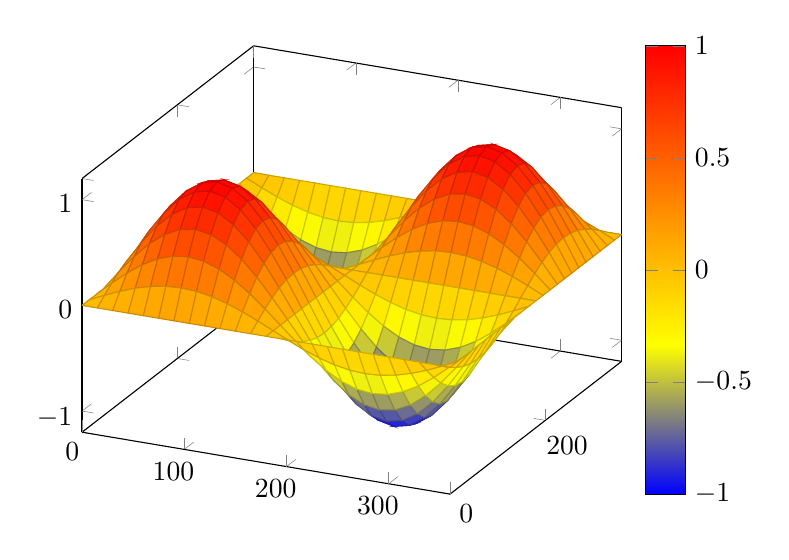
\begin{tikzpicture}
    \begin{axis}[colorbar]
      \addplot3[surf,domain=0:360]
      {sin(x)*sin(y)};
    \end{axis}
  \end{tikzpicture}
  \caption{Représentation graphique de la fonction $f:(x,y)\mapsto
    \sin x\times\sin y$}
  \label{sin-x*sin-y}
\end{figure}
%</developpementII-sample|flat-sample>
%</these-sample|flat-sample|flat-template|these-master|developpementII-sample>
%<*these-sample|flat-sample|flat-template|these-master>
%<<COMMENT
%
% Sixième chapitre
%COMMENT
%</these-sample|flat-sample|flat-template|these-master>
%<*these-sample|flat-sample|flat-template|these-master|conclusionII-sample>
%<flat-template>% \chapter{...}
%<flat-template>% ...
%<these-master>% \include{corps/}
%<these-sample>\include{corps/conclusionII}
%<*conclusionII-sample|flat-sample>
\chapter{Conclusion}
Dans ce chapitre, nous concluons l'étude du rire du chaos.

\lipsum[6-9]
%</conclusionII-sample|flat-sample>
%</these-sample|flat-sample|flat-template|these-master|conclusionII-sample>
%<*these-sample|flat-sample|flat-template|these-master>
%<<COMMENT
%
% Chapitre  de conclusion (générale)
%%%%%%%%%%%%%%%%%%%%%%%%%%%%%%%%%%%%%%%%%%%%%%%%%%%%%%%%%%%%%%%%%%%%%%%%%%%%%%%
%COMMENT
%</these-sample|flat-sample|flat-template|these-master>
%<*these-sample|flat-sample|flat-template|these-master|conclusion-master|conclusion-sample>
%<flat-template|conclusion-master>\chapter*{Conclusion}
%<flat-template|conclusion-master>% ...
%<these-sample|these-master>\section{Conclusion and future work}
\label{sec:conclusion}

Current rule-based query optimizers do not provide a very intuitive and
conceptually streamlined framework to define rules and actions.  Our
experiences with the Volcano optimizer generator suggest that its model
of rules and the expression of these rules is much more complicated and
too low-level than it needs to be.  As a consequence, rule sets in
Volcano are fragile, hard to write, and debug.  Similar problems may
exist in other contemporary rule-based query optimizers.

We believe that rule-based query optimizers will be standard tools
of future database systems.  The pragmatic difficulties of using
existing rule-based optimizers led us to develop Prairie, an
extensible and structured algebraic framework for specifying rules.
Prairie is similar to existing optimizers in that it supports both
transformation rules and implementation rules.  However, Prairie
makes several improvements:
\begin{enumerate}
\item it offers a conceptually more streamlined model for rule specification;
\item rules are encapsulated, there are no ``hidden'' operators or
      ``hidden'' algorithms;
\item implementation hints (\eg enforcers) are deduced automatically;
\item and it has efficient implementations.
\end{enumerate}

We have explained how the first three points are important for
simplifying rule specifications and making rule sets less brittle for
extensibility.  A consequence is that Prairie rules are simpler and
more robust than rules of existing optimizers (\eg Volcano).  We
addressed the fourth point by building a P2V pre-processor which uses
sophisticated algorithms to compose and compact a Prairie rule set into
a Volcano rule set.  To demonstrate the scalability of our approach, we
rewrote the TI Open OODB rule set as a Prairie rule set, generated its
Volcano counterpart, and showed that the performance of the synthesized
Volcano rule set closely matches the hand-crafted Volcano rule set.

Our future work will concentrate on developing higher-level
abstractions using Prairie, including automatically generating Prairie
rule sets, and combining multiple Prairie rule sets to automatically
generate efficient optimizers.

\section*{Acknowledgments}
\label{sec:acknowledgments}

We wish to thank Texas Instruments, Inc.\ for making the Open OODB
source code available to us.  Comments by Jos\'e Blakeley, Anne Ngu,
Vivek Singhal, Thomas Woo and the anonymous referees greatly improved
the quality of the paper.

%<*conclusion-sample|flat-sample>
\chapter*{Conclusion générale}
\lipsum[26-27]
\section{Une section de conclusion}
\lipsum[28-29]
\subsection{Une sous-section de conclusion}
\lipsum[29-31]
\subsubsection{Une sous-sous-section de conclusion}
\lipsum[31-35]
\paragraph{Un paragraphe de conclusion}
\lipsum[36-38]
\subparagraph{Un sous-paragraphe de conclusion}
\lipsum[39-41]
\subparagraph{Un autre sous-paragraphe de conclusion}
\lipsum[39-41]
\paragraph{Un autre paragraphe de conclusion}
\lipsum[36-38]
\subsubsection{Une autre sous-sous-section de conclusion}
\lipsum[31-37]
\subsection{Une autre sous-section de conclusion}
\lipsum[29-31]
\section{Une autre section de conclusion}
\lipsum[28-43]
%</conclusion-sample|flat-sample>
%</these-sample|flat-sample|flat-template|these-master|conclusion-master|conclusion-sample>
%<*these-sample|flat-sample|flat-template|these-master>
%<<COMMENT
%
% Liste des références bibliographiques
%COMMENT
%<flat-sample|these-sample>\printbibliography
%<flat-template|these-master>%\printbibliography
%<<COMMENT
%
%%%%%%%%%%%%%%%%%%%%%%%%%%%%%%%%%%%%%%%%%%%%%%%%%%%%%%%%%%%%%%%%%%%%%%%%%%%%%%%
% Début de la partie annexe éventuelle
%%%%%%%%%%%%%%%%%%%%%%%%%%%%%%%%%%%%%%%%%%%%%%%%%%%%%%%%%%%%%%%%%%%%%%%%%%%%%%%
%COMMENT
%<flat-template|these-master>% \appendix
%<these-sample|flat-sample>\appendix
%<<COMMENT
%
% Premier chapitre annexe (éventuel)
%COMMENT
%</these-sample|flat-sample|flat-template|these-master>
%<*flat-template|annexe-masterI>
%<<COMMENT
% \chapter{...}
% ...
%COMMENT
%</flat-template|annexe-masterI>
%<*these-sample|flat-sample|flat-template|these-master>
%<these-master>% \include{annexes/annexeI}
%<these-sample>\include{annexes/juridique}
%</these-sample|flat-sample|flat-template|these-master>
%<*juridique-sample|flat-sample>
\chapter{Documents juridiques}
\label{chap-juridique}

Cette partie regroupe les documents juridiques officiels.

\section{Licence sous laquelle est publié notre travail}
\label{sec-discours}

\lipsum[11-30]

\section{Transposition de la licence précédente en droit français}
\label{sec-autre-discours}

\lipsum[31-50]
%</juridique-sample|flat-sample>
%<*these-sample|flat-sample|flat-template|these-master>
%<<COMMENT
%
% Deuxième chapitre annexe (éventuel)
%COMMENT
%</these-sample|flat-sample|flat-template|these-master>
%<*flat-template|annexe-masterII>
%<<COMMENT
% \chapter{...}
% ...
%COMMENT
%</flat-template|annexe-masterII>
%<*these-sample|flat-sample|flat-template|these-master>
%<these-master>% \include{annexes/annexeII}
%<these-sample>% \iffalse
%
% Trademarks appear throughout this documentation without any trademark
% symbol, so you can't assume that a name is free. There is no intention
% of infringement; the usage is to the benefit of the trademark owner.
%
%
%  S O F T W A R E   L I C E N S E
% =================================
%
% The files  listings.dtx  and  listings.ins  and all files generated
% from only these two files are referred to as `the listings package'
% or simply `the package'. lstdrvrs.dtx  and the files generated from
% that file are `drivers'.
%
% The listings package is copyright 1996--2004 Carsten Heinz, and
% continued maintenance on the package is copyright 2006--2007 Brooks
% Moses. From 2013 on copyright is Jobst Hoffmann, who is the maintainer
% since july 2013. The drivers are copyright 1997/1998/1999/2000/2001/
% 2002/2003/2004/2006/2007/2013 any individual author listed in the
% driver files.
%
% The listings package and its drivers may be distributed and/or modified
% under the conditions of the LaTeX Project Public License, either version
% 1.3 of this license or (at your option) any later version.
% The latest version of this license is in
%   http://www.latex-project.org/lppl.txt
% and version 1.3 or later is part of all distributions of LaTeX
% version 2003/12/01 or later.
%
% The package has the LPPL maintenance status "maintained".
%
% $Id: listings.dtx 201 2015-06-04 20:25:39Z j_hoffmann $
%
% The Current Maintainer is Jobst Hoffmann <j.hoffmann(at)fh-aachen.de>.
%
% end of software license
%
%
%<*driver>
\documentclass[a4paper]{ltxdoc}
\DisableCrossrefs
\OnlyDescription

\usepackage{lstdoc,textcomp}
\usepackage{mdframed}           % frames for external files
\usepackage{moreverb}           % writing external files
\usepackage{xcolor}             % because of colouring the background

\makeindex

\begin{document}
    \DocInput{listings.dtx}
\end{document}
%</driver>
% \fi
%
%^^A
%^^A  Command/key to aspect relation
%^^A ================================
%^^A
%\lstisaspect[strings]{string,morestring,deletestring,stringstyle,showstringspaces}
%\lstisaspect[comments]{comment,morecomment,deletecomment,commentstyle}
%\lstisaspect[comment styles]{b,d,l,n,s,ib,id,il,in,is}
%\lstisaspect[pod]{printpod,podcomment}
%\lstisaspect[escape]{texcl,escapebegin,escapeend,escapechar,escapeinside,mathescape}
%\lstisaspect[keywords]{sensitive,classoffset,keywords,morekeywords,deletekeywords,keywordstyle,ndkeywords,morendkeywords,deletendkeywords,ndkeywordstyle,keywordsprefix,otherkeywords}
%\lstisaspect[emph]{emph,moreemph,deleteemph,emphstyle}
%\lstisaspect[tex]{texcs,moretexcs,deletetexcs,texcsstyle}
%\lstisaspect[directives]{directives,moredirectives,deletedirectives,directivestyle}
%\lstisaspect[html]{tag,usekeywordsintag,tagstyle,markfirstintag}
%\lstisaspect[keywordcomments]{keywordcomment,morekeywordcomment,deletekeywordcomment,keywordcommentsemicolon}
%\lstisaspect[index]{index,moreindex,deleteindex,indexstyle,\string\lstindexmacro}
%\lstisaspect[procnames]{procnamestyle,indexprocnames,procnamekeys,moreprocnamekeys,deleteprocnamekeys}
%\lstisaspect[style]{style,\string\lstdefinestyle,\string\lst@definestyle,\string\lststylefiles}
%\lstisaspect[language]{language,alsolanguage,defaultdialect,\string\lstalias,\string\lstdefinelanguage,\string\lst@definelanguage,\string\lstloadlanguages,\string\lstlanguagefiles}
%\lstisaspect[formats]{format,fmtindent,\string\lstdefineformat,\string\lst@defineformat,\string\lstformatfiles}
%\lstisaspect[labels]{numbers,numberstyle,numbersep,stepnumber,numberblanklines,firstnumber,\string\thelstnumber,numberfirstline}
%\lstisaspect[lineshape]{xleftmargin,xrightmargin,resetmargins,linewidth,lineskip,breaklines,breakindent,breakautoindent,prebreak,postbreak,breakatwhitespace}
%\lstisaspect[frames]{framexleftmargin,framexrightmargin,framextopmargin,framexbottommargin,backgroundcolor,fillcolor,rulecolor,rulesepcolor,rulesep,framerule,framesep,frameshape,frameround,frame}
%\lstisaspect[make]{makemacrouse}
%\lstisaspect[fancyvrb]{fancyvrb,fvcmdparams,morefvcmdparams}
%\lstisaspect[lgrind]{lgrindef,\string\lstlgrindeffile}
%\lstisaspect[hyper]{hyperref,morehyperref,deletehyperref,hyperanchor,hyperlink}
%\lstisaspect[kernel]{basewidth,fontadjust,columns,flexiblecolumns,identifierstyle,^^A
%   tabsize,showtabs,tab,showspaces,keepspaces,formfeed,SelectCharTable,^^A
%   MoreSelectCharTable,extendedchars,alsoletter,alsodigit,alsoother,excludedelims,^^A
%   literate,basicstyle,print,firstline,lastline,linerange,nolol,captionpos,abovecaptionskip,^^A
%   belowcaptionskip,label,title,caption,\string\lstlistingname,boxpos,float,^^A
%   floatplacement,aboveskip,belowskip,everydisplay,showlines,emptylines,gobble,name,^^A
%   \string\lstname,\string\lstlistlistingname,\string\lstlistoflistings,^^A
%   \string\lstnewenvironment,\string\lstinline,\string\lstinputlisting,lstlisting,^^A
%   \string\lstloadaspects,\string\lstset,\string\thelstlisting,\string\lstaspectfiles,^^A
%   inputencoding,delim,moredelim,deletedelim,upquote,numberbychapter,^^A
%   \string\lstMakeShortInline,\string\lstDeleteShortInline}
%\lstisaspect[doc]{lstsample,lstxsample}^^A environment
%\lstisaspect[experimental]{includerangemarker,rangebeginprefix,rangebeginsuffix,rangeendprefix,rangeendsuffix,rangeprefix,rangesuffix}
%
%^^A
%^^A  The long awaited beginning of documentation
%^^A =============================================
%^^A
%\newbox\abstractbox
%\setbox\abstractbox=\vbox{
%	\begin{abstract}
%	The \packagename{listings} package is a source code printer for \LaTeX.
%	You can typeset stand alone files as well as listings with an environment
%   similar to \texttt{verbatim} as well as you can print code snippets using
%   a command similar to |\verb|.
%	Many parameters control the output and if your preferred programming
%   language isn't already supported, you can make your own definition.
%	\end{abstract}}
%
% \title{\vspace*{-2\baselineskip}The \textsf{Listings} Package}
% \author{Copyright 1996--2004, Carsten Heinz%
%    \\ Copyright 2006--2007, Brooks Moses
%    \\ Copyright 2013--, Jobst Hoffmann
%    \\ Maintainer: Jobst Hoffmann\thanks{Jobst %
%       Hoffmann became the maintainer of the \packagename{listings}
%       package in 2013; see the Preface for details.}~ %
%    \textless\lstemail\textgreater}
% \date{2015/06/04\enspace\enspace Version 1.6\ \box\abstractbox}
% \def\lstemail{\href{mailto:j.hoffmann@fh-aachen.de}{\texttt{j.hoffmann(at)fh-aachen.de}}}
% \ifhyper
%    \hypersetup{pdfsubject=Package guide,pdfauthor=Jobst Hoffmann <j.hoffmann(at)fh-aachen.de>}
% \fi
%
% \csname @twocolumntrue\endcsname
% \maketitle
%^^A \enlargethispage{2\baselineskip}
% \csname @starttoc\endcsname{toc}
% \onecolumn
%
%
% \section*{Preface}
%
% \paragraph{Transition of package maintenance}
% The \TeX\ world lost contact with Carsten Heinz in late 2004, shortly after
% he released version 1.3b of the \packagename{listings} package.  After many
% attempts to reach him had failed, Hendri Adriaens took over maintenance of
% the package in accordance with the LPPL's procedure for abandoned packages.
% He then passed the maintainership of the package to Brooks Moses, who had
% volunteered for the position while this procedure was going through. The
% result is known as listings version 1.4.
%
% This release, version 1.5, is a minor maintenance release since
% I accepted maintainership of the package.  I would like to thank Stephan
% Hennig who supported the Lua language definitions. He is the one who
% asked for the integration of a new language and gave the impetus to me to
% become the maintainer of this package.
%
%
% \paragraph{News and changes}
% Version 1.5 is the fifth bugfix release.  There are no changes
% in this version, but two extensions: support of modern Fortran (2003,
% 2008) and Lua.
%
%
% \vfill
% \paragraph{Thanks}
% There are many people I have to thank for fruitful communication, posting
% their ideas, giving error reports, adding programming languages to
% \texttt{lstdrvrs.dtx}, and so on. Their names are listed in section
% \ref{uClosingAndCredits}.
%
% \paragraph{Trademarks}
% Trademarks appear throughout this documentation without any trademark
% symbol; they are the property of their respective trademark owner.
% There is no intention of infringement; the usage is to the benefit of the
% trademark owner.
%
%
% \clearpage
%
%
% \part{User's guide}
%
%
% \section{Getting started}\label{uGettingStarted}
%
%
% \subsection{A minimal file}\label{uAMinimalFile}
%
% Before using the \packagename{listings} package, you should be familiar with
% the \LaTeX\ typesetting system. You need not to be an expert.
% Here is a minimal file for \packagename{listings}.
% \begin{verbatim}
%    \documentclass{article}
%    \usepackage{listings}
%
%    \begin{document}
%    \lstset{language=Pascal}
%
%      % Insert Pascal examples here.
%
%    \end{document}\end{verbatim}
% Now type in this first example and run it through \LaTeX.
% \begin{advise}
% \item Must I do that really?
%       \advisespace
%       Yes and no. Some books about programming say this is good.
%       What a mistake! Typing takes time---which is wasted if the code is clear to
%       you. And if you need that time to understand what is going on, the
%       author of the book should reconsider the concept of presenting the
%       crucial things---you might want to say that about this guide even---or
%       you're simply inexperienced with programming. If only the latter case
%       applies, you should spend more time on reading (good) books about
%       programming, (good) documentations, and (good) source code from other
%       people. Of course you should also make your own experiments.
%       You will learn a lot. However, running the example through \LaTeX\
%       shows whether the \packagename{listings} package is installed correctly.
% \item The example doesn't work.
%       \advisespace
%       Are the two packages \packagename{listings} and \packagename{keyval}
%       installed on your system? Consult the administration tool of your
%       \TeX\ distribution, your system administrator, the local \TeX\ and
%       \LaTeX\ guides, a \TeX\ FAQ, and section \ref{rInstallation}---in
%       that order. If you've checked \emph{all} these sources and are
%       still helpless, you might want to write a post to a \TeX\ newsgroup
%       like \texttt{comp.text.tex}.
% \item Should I read the software license before using the package?
%       \advisespace
%       Yes, but read this \emph{Getting started} section first to decide
%       whether you are willing to use the package.^^A ;-)
% \end{advise}
%
%
% \subsection{Typesetting listings}
%
% Three types of source codes are supported: code snippets, code segments, and
% listings of stand alone files.  Snippets are placed inside paragraphs and the
% others as separate paragraphs---the difference is the same as between text
% style and display style formulas.
% \begin{advise}
% \item No matter what kind of source you have, if a listing contains national
%       characters like \'e, \L, \"a, or whatever, you must tell the
%       package about it! Section \lstref{uSpecialCharacters} discusses this issue.
% \end{advise}
%
% \paragraph{Code snippets}
% The well-known \LaTeX\ command |\verb| typesets code snippets verbatim.
% The new command |\lstinline| pretty-prints the code, for example
%`\lstinline!var i:integer;!' is typeset by
%`{\rstyle|\lstinline|}|!var i:integer;!|'. The exclamation marks delimit
% the code and can be replaced by any character not in the code;
% |\lstinline$var i:integer;$| gives the same result.
%
% \paragraph{Displayed code}
% The \texttt{lstlisting} environment typesets the enclosed source code. Like
% most examples, the following one shows verbatim \LaTeX\ code on the right
% and the result on the left. You might take the right-hand side, put it into
% the minimal file, and run it through \LaTeX.
% \begin{lstsample}[lstlisting]{}{}
%    \begin{lstlisting}
%    for i:=maxint to 0 do
%    begin
%        { do nothing }
%    end;
%
%    Write('Case insensitive ');
%    WritE('Pascal keywords.');
%    \end{lstlisting}
% \end{lstsample}
% It can't be easier.
% \begin{advise}
% \item That's not true. The name `\texttt{listing}' is shorter.
%       \advisespace
%       Indeed. But other packages already define environments with that name.
%       To be compatible with such packages, all commands and environments of
%       the \packagename{listings} package use the prefix `\texttt{lst}'.
% \end{advise}
% The environment provides an optional argument. It tells the package to
% perform special tasks, for example, to print only the lines 2--5:
% \begin{lstsample}{\lstset{frame=trbl,framesep=0pt}\label{gFirstKey=ValueList}}{}
%    \begin{lstlisting}[firstline=2,
%                       lastline=5]
%    for i:=maxint to 0 do
%    begin
%        { do nothing }
%    end;
%
%    Write('Case insensitive ');
%    WritE('Pascal keywords.');
%    \end{lstlisting}
% \end{lstsample}
% \begin{advise}
% \item Hold on! Where comes the frame from and what is it good for?
%       \advisespace
%       You can put frames around all listings except code snippets.
%       You will learn how later. The frame shows that empty lines at the end
%       of listings aren't printed. This is line 5 in the example.
% \item Hey, you can't drop my empty lines!
%       \advisespace
%       You can tell the package not to drop them:
%       The key `\ikeyname{showlines}' controls these empty lines and is
%       described in section \ref{rTypesettingListings}. Warning: First
%       read ahead on how to use keys in general.
% \item I get obscure error messages when using `\ikeyname{firstline}'.
%       \advisespace
%       That shouldn't happen. Make a bug report as described in section
%       \lstref{uTroubleshooting}.
% \end{advise}
%
% \paragraph{Stand alone files}
% Finally we come to |\lstinputlisting|, the command used to pretty-print
% stand alone files. It has one optional and one file name argument.
% Note that you possibly need to specify the relative path to the file.
% Here now the result is printed below the verbatim code since both together
% don't fit the text width.
% \begin{lstsample}{\lstset{comment=[l]\%,columns=fullflexible}}{\lstset{alsoletter=\\,emph=\\lstinputlisting,emphstyle=\rstyle}\lstaspectindex{\lstinputlisting}{}}
%    \lstinputlisting[lastline=4]{listings.sty}
% \end{lstsample}
% \begin{advise}
% \item The spacing is different in this example.
%       \advisespace
%       Yes. The two previous examples have aligned columns, i.e.~columns with
%       identical numbers have the same horizontal position---this package
%       makes small adjustments only. The columns in the example here are not
%       aligned. This is explained in section \ref{uFixedAndFlexibleColumns}
%       (keyword: full flexible column format).
% \end{advise}
%
% Now you know all pretty-printing commands and environments. It remains
% to learn the parameters which control the work of the \packagename{listings}
% package. This is, however, the main task. Here are some of them.
%
%
% \subsection{Figure out the appearance}\label{gFigureOutTheAppearance}
%
% Keywords are typeset bold, comments in italic shape, and spaces in strings
% appear as \textvisiblespace. You don't like these settings? Look at this:
%\ifcolor
% \begin{lstxsample}[basicstyle,keywordstyle,identifierstyle,commentstyle,stringstyle,showstringspaces]
%    \lstset{% general command to set parameter(s)
%        basicstyle=\small,          % print whole listing small
%        keywordstyle=\color{black}\bfseries\underbar,
%                                    % underlined bold black keywords
%        identifierstyle=,           % nothing happens
%        commentstyle=\color{white}, % white comments
%        stringstyle=\ttfamily,      % typewriter type for strings
%        showstringspaces=false}     % no special string spaces
% \end{lstxsample}
%\else
% \begin{lstxsample}[basicstyle,keywordstyle,identifierstyle,commentstyle,stringstyle,showstringspaces]
%    \lstset{% general command to set parameter(s)
%        basicstyle=\small,          % print whole listing small
%        keywordstyle=\bfseries\underbar,
%                                    % underlined bold keywords
%        identifierstyle=,           % nothing happens
%        commentstyle=\itshape,      % default
%        stringstyle=\ttfamily,      % typewriter type for strings
%        showstringspaces=false}     % no special string spaces
% \end{lstxsample}
%\fi
% \begin{lstsample}{}{}
%    \begin{lstlisting}
%    for i:=maxint to 0 do
%    begin
%        { do nothing }
%    end;
%
%    Write('Case insensitive ');
%    WritE('Pascal keywords.');
%    \end{lstlisting}
% \end{lstsample}
%\ifcolor
% \begin{advise}
% \item You've requested white coloured comments, but I can see the comment
%       on the left side.
%       \advisespace
%       There are a couple of possible reasons:
%       (1) You've printed the documentation on nonwhite paper.
%       (2) If you are viewing this documentation as a \texttt{.dvi}-file, your
%           viewer seems to have problems with colour specials. Try to print
%           the page on white paper.
%       (3) If a printout on white paper shows the comment, the colour
%           specials aren't suitable for your printer or printer driver.
%           Recreate the documentation and try it again---and ensure that
%           the \packagename{color} package is well-configured.
% \end{advise}
%\fi
% The styles use two different kinds of commands. |\ttfamily| and |\bfseries|
% both take no arguments but |\underbar| does; it underlines the following
% argument. In general, the \emph{very last} command may read exactly one
% argument, namely some material the package typesets. There's one exception.
% The last command of \ikeyname{basicstyle} \emph{must not} read any
% tokens---or you will get deep in trouble.
% \begin{advise}
% \item `|basicstyle=\small|' looks fine, but comments look really bad with
%       `|commentstyle=\tiny|' and empty basic style, say.
%       \advisespace
%       Don't use different font sizes in a single listing.
% \item But I really want it!
%       \advisespace
%       No, you don't.
%^^A       The package adjusts internal data after selecting the basic style at
%^^A       the beginning of each listing. This is a problem if you change the
%^^A       font size for comments or strings, for example.
%^^A       Section \ref{rColumnAlignment} shows how to overcome this.
%^^A       But once again: Don't use different font sizes in a single listing
%^^A       unless you really know what you are doing.
% \end{advise}
%
% \paragraph{Warning}\label{wStrikingStyles}
% You should be very careful with striking styles; the recent example is rather
% moderate---it can get horrible. \emph{Always use decent highlighting.}
% Unfortunately it is difficult to give more recommendations since they depend
% on the type of document you're creating. Slides or other presentations often
% require more striking styles than books, for example.
% In the end, it's \emph{you} who have to find the golden mean!
%
%
% \subsection{Seduce to use}\label{gSeduceToUse}
%
% You know all pretty-printing commands and some main parameters. Here now
% comes a small and incomplete overview of other features. The table of
% contents and the index also provide information.
%
% \paragraph{Line numbers}
% are available for all displayed listings, e.g.~tiny numbers on the left, each
% second line, with 5pt distance to the listing:
% \begin{lstxsample}[numbers,numberstyle,stepnumber,numbersep]
%    \lstset{numbers=left, numberstyle=\tiny, stepnumber=2, numbersep=5pt}
% \end{lstxsample}
% \begin{lstsample}{}{}
%    \begin{lstlisting}
%    for i:=maxint to 0 do
%    begin
%        { do nothing }
%    end;
%
%    Write('Case insensitive ');
%    WritE('Pascal keywords.');
%    \end{lstlisting}
% \end{lstsample}
% \begin{advise}
% \item I can't get rid of line numbers in subsequent listings.
%       \advisespace
%       `|numbers=none|' turns them off.
% \item Can I use these keys in the optional arguments?
%       \advisespace
%       Of course. Note that optional arguments modify values for one
%       particular listing only: you change the appearance, step or distance
%       of line numbers for a single listing. The previous values are
%       restored afterwards.
% \end{advise}
% The environment allows you to interrupt your listings: you can end a listing
% and continue it later with the correct line number even if there are other
% listings in between. Read section \ref{uLineNumbers} for a thorough
% discussion.
%
% \paragraph{Floating listings}
% Displayed listings may float:
% \begin{lstsample}{\lstset{frame=tb}}{}
%    \begin{lstlisting}[float,caption=A floating example]
%    for i:=maxint to 0 do
%    begin
%        { do nothing }
%    end;
%
%    Write('Case insensitive ');
%    WritE('Pascal keywords.');
%    \end{lstlisting}
% \end{lstsample}
% Don't care about the parameter \ikeyname{caption} now. And if you put the
% example into the minimal file and run it through \LaTeX, please don't wonder:
% you'll miss the horizontal rules since they are described elsewhere.
% \begin{advise}
% \item \LaTeX's float mechanism allows one to determine the placement of floats.
%       How can I do that with these?
%       \advisespace
%       You can write `|float=tp|', for example.
% \end{advise}
%
% \paragraph{Other features}
% There are still features not mentioned so far: automatic breaking of long
% lines, the possibility to use \LaTeX\ code in listings, automated indexing,
% or personal language definitions.
% One more little teaser? Here you are. But note that the result is not
% produced by the \LaTeX\ code on the right alone. The main parameter is
% hidden.
% \begin{lstsample}{\lstset{literate={:=}{{$\gets$}}1 {<=}{{$\leq$}}1 {>=}{{$\geq$}}1 {<>}{{$\neq$}}1}}{}
%    \begin{lstlisting}
%    if (i<=0) then i := 1;
%    if (i>=0) then i := 0;
%    if (i<>0) then i := 0;
%    \end{lstlisting}
% \end{lstsample}
%
% You're not sure whether you should use \packagename{listings}?
% Read the next section!
%
%
% \subsection{Alternatives}
%
% \begin{advise}
% \item Why do you list alternatives?
%       \advisespace
%       Well, it's always good to know the competitors.^^A :-)
% \item I've read the descriptions below and the \packagename{listings} package
%       seems to incorporate all the features. Why should I use one of the
%       other programs?
%       \advisespace
%       Firstly, the descriptions give a taste and not a complete overview,
%       secondly, \packagename{listings} lacks some properties, and, ultimately,
%       you should use the program matching your needs most precisely.
% \end{advise}
% This package is certainly not the final utility for typesetting source code.
% Other programs do their job very well, if you are not satisfied with
% \packagename{listings}. Some are independent of \LaTeX, others come as
% separate program plus \LaTeX\ package, and others are packages which
% don't pretty-print the source code. The second type includes converters,
% cross compilers, and preprocessors. Such programs create \LaTeX\ files
% you can use in your document or stand alone ready-to-run \LaTeX\ files.
%
% Note that I'm not dealing with any literate programming tools here, which
% could also be alternatives. However, you should have heard of the
% \texttt{WEB} system, the tool Prof.~Donald E.~Knuth developed and made use
% of to document and implement \TeX.
%
% \paragraph{\href{http://www.infres.enst.fr/~demaille/a2ps}{\packagename{a2ps}}}
% started as `ASCII to PostScript' converter, but today you can invoke the
% program with \texttt{--pretty-print=}\meta{language} option. If your
% favourite programming language is not already supported, you can write your
% own so-called style sheet. You can request line numbers, borders, headers,
% multiple pages per sheet, and many more. You can even print symbols like
% $\forall$ or $\alpha$ instead of their verbose forms. If you just want
% program listings and not a document with some listings, this is the best
% choice.
%
% \paragraph{\href{http://www.ctan.org/tex-archive/nonfree/support/lgrind}{\packagename{LGrind}}}
% is a cross compiler and comes with many predefined programming languages.
% For example, you can put the code on the right in your document, invoke
% \packagename{LGrind} with \texttt{-e} option (and file names), and run the
% created file through \LaTeX. You should get a result similar to the
% left-hand side:
% \begin{center}
% \begin{minipage}{0.45\linewidth}
%\iflgrind
%    \LGindent=0pt
%    \LGinlinefalse\LGbegin\lgrinde
%    \L{\LB{\K{for}_\V{i}:=\V{maxint}_\K{to}_\N{0}_\K{do}}}
%    \L{\LB{\K{begin}}}
%    \L{\LB{____\C{}\{_do_nothing_\}\CE{}}}
%    \L{\LB{\K{end};}}
%    \L{\LB{}}
%    \L{\LB{\V{Write}(\S{}{'}Case_insensitive_{'}\SE{});}}
%    \L{\LB{\V{WritE}(\S{}{'}Pascal_keywords.{'}\SE{});}}
%    \endlgrinde\LGend
%\else
%    \packagename{LGrind} not installed.
%\fi
% \end{minipage}
% \begin{minipage}{0.45\linewidth}
% \begin{verbatim}
% %[
% for i:=maxint to 0 do
% begin
%     { do nothing }
% end;
%
% Write('Case insensitive ');
% WritE('Pascal keywords.');
% %]\end{verbatim}
% \end{minipage}
% \end{center}
% If you use |%(| and |%)| instead of |%[| and |%]|, you get a code snippet
% instead of a displayed listing. Moreover you can get line numbers to the
% left or right, use arbitrary \LaTeX\ code in the source code, print symbols
% instead of verbose names, make font setup, and more. You will (have to)
% like it (if you don't like \packagename{listings}).
%
% Note that \packagename{LGrind} contains code with a no-sell license and is
% thus nonfree software.
%
% \paragraph{\href{ftp://axp3.sv.fh-mannheim.de/cvt2latex}{\packagename{cvt2ltx}}}
% is a family of `source code to \LaTeX' converters for C, Objective C, \Cpp,
% IDL and Perl. Different styles, line numbers and other qualifiers can be
% chosen by command-line option. Unfortunately it isn't documented how other
% programming languages can be added.
%
% \paragraph{\href{http://www.ctan.org/tex-archive/support/C++2LaTeX-1_1pl1}{\packagename{\Cpp2\LaTeX}}}
% is a C/\Cpp\ to \LaTeX\ converter. You can specify the fonts for comments,
% directives, keywords, and strings, or the size of a tabulator. But as far as
% I know you can't number lines.
%
% \paragraph{\href{http://www.ctan.org/tex-archive/support/slatex}{\packagename{S\LaTeX}}}
% is a pretty-printing Scheme program (which invokes \LaTeX\ automatically)
% especially designed for Scheme and other Lisp dialects. It supports stand
% alone files, text and display listings, and you can even nest the
% commands/environments if you use \LaTeX\ code in comments, for example.
% Keywords, constants, variables, and symbols are definable and use of
% different styles is possible. No line numbers.
%
% \paragraph{\href{http://www.ctan.org/tex-archive/support/tiny_c2l}{\packagename{tiny\textunderscore c2ltx}}}
% is a C/\Cpp/Java to \LaTeX\ converter based on \packagename{cvt2ltx} (or the
% other way round?). It supports line numbers, block comments, \LaTeX\ code
% in/as comments, and smart line breaking. Font selection and tabulators are
% hard-coded, i.e.~you have to rebuild the program if you want to change the
% appearance.
%
% \paragraph{\href{http://www.ctan.org/tex-archive/macros/latex/contrib/misc}{\packagename{listing}}}
% ---note the missing \packagename{s}---is not a pretty-printer and the
% aphorism about documentation at the end of \texttt{listing.sty} is not
% true.\space ^^A :-)
% It defines |\listoflistings| and a nonfloating environment for listings.
% All font selection and indention must be done by hand. However, it's
% useful if you have another tool doing that work, e.g.~\packagename{LGrind}.
%
% \paragraph{\href{http://www.ctan.org/tex-archive/macros/latex/contrib/alg}{\packagename{alg}}}
% provides essentially the same functionality as \packagename{algorithms}.
% So read the next paragraph and note that the syntax will be different.
%
% \paragraph{\href{http://www.ctan.org/tex-archive/macros/latex/contrib/algorithms}{\packagename{algorithms}}}
% goes a quite different way. You describe an algorithm and the package
% formats it, for example
% \begin{center}
% \begin{minipage}{0.45\linewidth}
%\ifalgorithmicpkg
%    \begin{algorithmic}
%    \IF {$i\leq0$}
%    \STATE $i\gets1$
%    \ELSE\IF {$i\geq0$}
%    \STATE $i\gets0$
%    \ENDIF\ENDIF
%    \end{algorithmic}
%\else
%    \packagename{algorithms} not installed.
%\fi
% \end{minipage}
% \begin{minipage}{0.45\linewidth}
% \begin{verbatim}
%\begin{algorithmic}
%\IF{$i\leq0$}
%\STATE $i\gets1$
%\ELSE\IF{$i\geq0$}
%\STATE $i\gets0$
%\ENDIF\ENDIF
%\end{algorithmic}\end{verbatim}
% \end{minipage}
% \end{center}
% As this example shows, you get a good looking algorithm even from a bad
% looking input. The package provides a lot more constructs like |for|-loops,
% |while|-loops, or comments. You can request line numbers, `ruled', `boxed'
% and floating algorithms, a list of algorithms, and you can customize the
% terms \textbf{if}, \textbf{then}, and so on.
%
% \paragraph{\href{http://www.mimuw.edu.pl/~wolinski/pretprin.html}{\packagename{pretprin}}}
% is a package for pretty-printing texts in formal languages---as the title
% in TUGboat, Volume 19 (1998), No.~3 states. It provides environments which
% pretty-print \emph{and} format the source code. Analyzers for Pascal and
% Prolog are defined; adding other languages is easy---if you are or get a bit
% familiar with automatons and formal languages.
%
% \paragraph{\packagename{alltt}}
% defines an environment similar to \texttt{verbatim} except that |\|, |{| and
% |}| have their usual meanings. This means that you can use commands in the
% verbatims, e.g.~select different fonts or enter math mode.
%
% \paragraph{\href{http://www.ctan.org/tex-archive/macros/latex/contrib/moreverb}{\packagename{moreverb}}}
% requires \packagename{verbatim} and provides verbatim output to a file,
% `boxed' verbatims and line numbers.
%
% \paragraph{\packagename{verbatim}}
% defines an improved version of the standard \texttt{verbatim} environment and
% a command to input files verbatim.
%
% \paragraph{\href{http://www.ctan.org/tex-archive/macros/latex/contrib/fancyvrb}{\packagename{fancyvrb}}}
% is, roughly speaking, a superset of \packagename{alltt},
% \packagename{moreverb}, and \packagename{verbatim}, but many more parameters
% control the output. The package provides frames, line numbers on the left or
% on the right, automatic line breaking (difficult), and more. For example, an
% interface to \packagename{listings} exists, i.e.~you can pretty-print source
% code automatically.
% The package \packagename{fvrb-ex} builds on \packagename{fancyvrb} and
% defines environments to present examples similar to the ones in this guide.
%
%
% \section{The next steps}\label{uTheNextSteps}
%
% Now, before actually using the \packagename{listings} package, you should
% \emph{really} read the software license. It does not cost much time and
% provides information you probably need to know.
%
%
% \subsection{Software license}\label{uSoftwareLicense}
%
% The files \texttt{listings.dtx} and \texttt{listings.ins} and all
% files generated from only these two files are referred to as `the
% \packagename{listings} package' or simply `the package'.
% \texttt{lstdrvrs.dtx} and the files generated from that file are
% `drivers'.
%
% \paragraph{Copyright}
%   The \packagename{listings} package is copyright 1996--2004 Carsten Heinz,
%   and copyright 2006 Brooks Moses.  The drivers are copyright any individual
%   author listed in the driver files.
%
% \paragraph{Distribution and modification}
%   The \packagename{listings} package and its drivers may be distributed
%   and/or modified under the conditions of the LaTeX Project Public License,
%   either version 1.3 of this license or (at your option) any later version.
%   The latest version of this license is in
%      \href{http://www.latex-project.org/lppl.txt}{http://www.latex-project.org/lppl.txt}
%   and version 1.3 or later is part of all distributions of LaTeX version
%  2003/12/01 or later.
%
% \paragraph{Contacts}
%   Read section \lstref{uTroubleshooting} on how to submit a bug report.
%   Send all other comments, ideas, and additional programming languages to
%   \lstemail\ using \texttt{listings} as part of the subject.
%
%
% \subsection{Package loading}\label{uPackageLoading}
%
% As usual in \LaTeX, the package is loaded by
%    |\usepackage[|\meta{options}|]{listings}|,
% where |[|\meta{options}|]| is optional and gives a comma separated list of
% options. Each either loads an additional \packagename{listings} aspect, or
% changes default properties. Usually you don't have to take care of such
% options. But in some cases it could be necessary: if you want to compile
% documents created with an earlier version of this package or if you use
% special features. Here's an incomplete list of possible options.
% \begin{advise}
% \item Where is a list of all of the options?
%       \advisespace
%       In the developer's guide since they were introduced to debug the
%       package more easily. Read section \ref{uHowTos} on how to get that
%       guide.
% \end{advise}
% \begin{description}
% \item[\normalfont\texttt{0.21}]\leavevmode
%
%       invokes a compatibility mode for compiling documents written for
%       \packagename{listings} version 0.21.
%
% \item[\normalfont\texttt{draft}]\leavevmode
%
%       The package prints no stand alone files, but shows the captions and
%       defines the corresponding labels.
%       Note that a global |\documentclass|-option \texttt{draft} is
%       recognized, so you don't need to repeat it as a package option.
%
% \item[\normalfont\texttt{final}]\leavevmode\label{uoption:final}
%
%       Overwrites a global \texttt{draft} option.
%
% \item[\normalfont\texttt{savemem}]\leavevmode
%
%       tries to save some of \TeX's memory. If you switch between languages
%       often, it could also reduce compile time. But all this depends on the
%       particular document and its listings.
% \end{description}
% Note that various experimental features also need explicit loading via
% options. Read the respective lines in section \ref{rExperimentalFeatures}.
%
% \medbreak
% After package loading it is recommend to load all used dialects of programming
% languages with the following command. It is faster to load several languages
% with one command than loading each language on demand.
% \begin{syntax}
% \item {\rstyle\icmdname\lstloadlanguages}\marg{comma separated list of languages}
%
%       Each language is of the form \oarg{dialect}\meta{language}. Without
%       the optional \oarg{dialect} the package loads a default dialect. So
%       write `|[Visual]C++|' if you want Visual \Cpp\ and `|[ISO]C++|' for
%       ISO \Cpp. Both together can be loaded by the command
%       |\lstloadlanguages{[Visual]C++,[ISO]C++}|.
%
%       Table \ref{uPredefinedLanguages} on page \pageref{uPredefinedLanguages}
%       shows all defined languages and their dialects.
% \end{syntax}
%^^A After or even before language loading, you might want to define default
%^^A dialects---just to be independent of configuration files.
%
%
% \subsection{The key=value interface}\label{uTheKey=ValueInterface}
%
% This package uses the \packagename{keyval} package from the
% \packagename{graphics} bundle by David Carlisle. Each parameter is
% controlled by an associated key and a user supplied value. For example,
% \ikeyname{firstline} is a key and |2| a valid value for this key.
%
% The command {\rstyle\icmdname\lstset} gets a comma separated list of
% ``key|=|value'' pairs. The first list with more than a single entry is on
% page \pageref{gFirstKey=ValueList}: |firstline=2,lastline=5|.
% \begin{advise}
% \item So I can write `|\lstset{firstline=2,lastline=5}|' once for all?
%       \advisespace
%       No. `\ikeyname{firstline}' and `\ikeyname{lastline}' belong to a small
%       set of
%       keys which are only used on individual listings. However, your command is
%       not illegal---it has no effect. You have to use these keys inside the
%       optional argument of the environment or input command.
% \item What's about a better example of a key|=|value list?
%       \advisespace
%       There is one in section \ref{gFigureOutTheAppearance}.
% \item `|language=[77]Fortran|' does not work inside an optional argument.
%       \advisespace
%       You must put braces around the value if a value with optional argument
%       is used inside an optional argument. In the case here write
%       `|language={[77]Fortran}|' to select Fortran 77.
% \item If I use the `\ikeyname{language}' key inside an optional argument, the
%       language isn't active when I typeset the next listing.
%       \advisespace
%       All parameters set via `|\lstset|' keep their values up to the end of
%       the current environment or group. Afterwards the previous values are
%       restored. The optional parameters of the two pretty-printing commands
%       and the `\texttt{lstlisting}' environment take effect on the particular
%       listing only, i.e.~values are restored immediately. For example, you
%       can select a main language and change it for special listings.
% \item \icmdname\lstinline\ has an optional argument?
%       \advisespace
%       Yes. And from this fact comes a limitation: you can't use the left
%       bracket `|[|' as delimiter unless you specify at least an empty
%       optional argument as in `|\lstinline[][var i:integer;[|'.
%       If you forget this, you will either get a ``runaway argument'' error
%       from \TeX, or an error message from the \packagename{keyval} package.
% \end{advise}
%
%
% \subsection{Programming languages}\label{uProgrammingLanguages}
%
% You already know how to activate programming languages---at least Pascal.
% An optional parameter selects particular dialects of a language. For example,
% |language=[77]Fortran| selects Fortran 77 and |language=[XSC]Pascal| does the
% same for Pascal XSC. The general form is
%    {\rstyle\ikeyname{language}}|=|\oarg{dialect}\meta{language}.
% If you want to get rid of keyword, comment, and string detection, use
% |language={}| as an argument to |\lstset| or as optional argument.
%
% Table \ref{uPredefinedLanguages} shows all predefined languages and dialects.
% Use the listed names as \meta{language} and \meta{dialect}, respectively. If
% no dialect or `empty' is given in the table, just don't specify a dialect.
% Each underlined dialect is default; it is selected if you leave out
% the optional argument. The predefined defaults are the newest language
% versions or standard dialects.
%^^A
%^^A  Make table of predefined languages.
%^^A
%\let\lstlanguages\empty
%\makeatletter
%\@for\lst@temp:={lstlang1.sty,lstlang2.sty,lstlang3.sty}\do
%    {\IfFileExists\lst@temp{}{\let\lstlanguages\relax}}
%\makeatother
%\ifx\lstlanguages\relax
%    \PackageWarningNoLine{Listings}
%        {Standard drivers not available.\MessageBreak
%         Please check your installation.\MessageBreak
%         Compilation aborted}
%    \csname @@end\expandafter\endcsname
%\fi
%\lstscanlanguages\lstlanguages{lstlang1.sty,lstlang2.sty,lstlang3.sty}{}^^A
%\def\topfigrule{\hrule\kern-0.4pt\relax}^^A
%\let\botfigrule\topfigrule
%\belowcaptionskip=\smallskipamount
% \begin{table}[tbhp]
% \small
% \caption{Predefined languages.
%          Note that some definitions are preliminary, for example HTML and XML.
%          Each underlined dialect is the default dialect.}^^A
%          \label{uPredefinedLanguages}^^A
% \makeatletter
% \setbox\@tempboxa\hbox{^^A
%    \InputIfFileExists{listings.cfg}{\lst@InputCatcodes}{}}^^A
% \lstprintlanguages\lstlanguages
% \end{table}
%^^A
%^^A end of table
%^^A
%\lstset{defaultdialect=[doc]Pascal}^^A restore
% \begin{advise}
% \item How can I define default dialects?
%       \advisespace
%       Check section \ref{rLanguagesAndStyles} for `\keyname{defaultdialect}'.
% \item I have C code mixed with assembler lines. Can \packagename{listings}
%       pretty-print such source code, i.e.~highlight keywords and comments of
%       both languages?
%       \advisespace
%       `\ikeyname{alsolanguage}|=|\oarg{dialect}\meta{language}' selects a
%       language additionally to the active one. So you only have to write a
%       language definition for your assembler dialect, which doesn't interfere
%       with the definition of C, say. Moreover you might want to use the key
%       `\keyname{classoffset}' described in section \ref{rLanguagesAndStyles}.
% \item How can I define my own language?
%       \advisespace
%       This is discussed in section \ref{rLanguageDefinitions}. And if you
%       think that other people could benefit by your definition, you might
%       want to send it to the address in section \ref{uSoftwareLicense}.
%       Then it will be published under the \LaTeX\ Project Public License.
% \end{advise}
% Note that the arguments \meta{language} and \meta{dialect} are case
% insensitive and that spaces have no effect.
%
% There is at least one language (VDM, Vienna Development Language,
% \url{http://www.vdmportal.org}) which is not directly supported by the
% \packagename{listings} package. It needs a package for its own:
% \packagename{vdmlisting}. On the other hand \packagename{vdmlisting} uses
% the \packagename{listings} package and so it should be mentioned in this
% context.
%
%
% \subsubsection{Preferences}\label{uPreferences}
%
% Sometimes authors of language support provide their own configuration
% preferences. These may come either from their personal experience or
% from the settings in an IDE and can be defined as a \packagename{listings}
% style. From version 1.5b of the \packagename{listings} package on these
% styles are provided as files with the name
% |listings-|\meta{language}|.prf|, \meta{language} is the name of the
% supported programming language in lowercase letters.
%
% So if an user of the \packagename{listings} package wants to use these
% preferences, she/he can say for example when using Python
% \begin{quote}
%     |\input{listings-python.prf}|
% \end{quote}
% at the end of her/his |listings.cfg| configuration file as long as the
% file |listings-python.prf| resides in the \TeX{} search path. Of course
% that file can be changed according to the user's preferences.
%
% At the moment there are five such preferences files:
% \begin{enumerate}
%   \item |listings-acm.prf|
%   \item |listings-bash.prf|
%   \item |listings-fortran.prf|
%   \item |listings-lua.prf|
%   \item |listings-python.prf|
% \end{enumerate}
% All contributors are invited to supply more personal preferences.
%
%
% \subsection{Special characters}\label{uSpecialCharacters}
%
%
% \paragraph{Tabulators}
% You might get unexpected output if your sources contain tabulators.
% The package assumes tabulator stops at columns 9, 17, 25, 33, and so on.
% This is predefined via |tabsize=8|. If you change the eight to the number
% $n$, you will get tabulator stops at columns $n+1,2n+1,3n+1,$ and so on.
% \begin{lstsample}[tabsize]{}{}
%    \lstset{tabsize=2}
%    \begin{lstlisting}
%    123456789
%    	{ one tabulator }
%    		{ two tabs }
%    123		{ 123 + two tabs }
%    \end{lstlisting}
% \end{lstsample}
% For better illustration, the left-hand side uses |tabsize=2| but the verbatim
% code |tabsize=4|. Note that |\lstset| modifies the values for all following
% listings in the same environment or group. This is no problem here since the
% examples are typeset inside minipages. If you want to change settings for a
% single listing, use the optional argument.
%
%
% \paragraph{Visible tabulators and spaces}
% One can make spaces and tabulators visible:
% \begin{lstsample}[showspaces,showtabs,tab]{}{}
%    \lstset{showspaces=true,
%            showtabs=true,
%            tab=\rightarrowfill}
%    \begin{lstlisting}
%        for i:=maxint to 0 do
%        begin
%    	{ do nothing }
%        end;
%    \end{lstlisting}
% \end{lstsample}
% If you request \ikeyname{showspaces} but no \ikeyname{showtabs},
% tabulators are converted to visible spaces.
% The default definition of \ikeyname{tab} produces a `wide visible space'
% \lstinline[showtabs]!	!. So you might want to use |$\to$|, |$\dashv$|
% or something else instead.
% \begin{advise}
% \item Some sort of advice: (1) You should really indent lines of source code
%       to make listings more readable. (2) Don't indent some lines with
%       spaces and others via tabulators. Changing the tabulator size (of your
%       editor or pretty-printing tool) completely disturbs the columns.
%       (3) As a consequence, never share your files with differently tab sized
%       people!^^A true only if you use tabulators, just :-)
% \item To make the \LaTeX\ code more readable, I indent the environments'
%       program listings. How can I remove that indention in the output?
%       \advisespace
%       Read `How to gobble characters' in section \ref{uHowTos}.
% \end{advise}
%
%
% \paragraph{Form feeds}
% Another special character is a form feed causing an empty line by default.
% {\rstyle\ikeyname{formfeed}}|=\newpage| would result in a new page every
% form feed. Please note that such definitions (even the default) might get
% in conflict with frames.
%
%
% \paragraph{National characters}
% If you type in such characters directly as characters of codes 128--255 and
% use them also in listings, let the package know it---or you'll get really
% funny results. {\rstyle\ikeyname{extendedchars}}|=true| allows and
% |extendedchars=false| prohibits \packagename{listings} from handling
% extended characters in listings. If you use them, you should load
% \packagename{fontenc}, \packagename{inputenc} and/or
% any other package which defines the characters.
% \begin{advise}
% \item I have problems using \packagename{inputenc} together with
%       \packagename{listings}.
%       \advisespace
%       This could be a compatibility problem. Make a bug report as described
%       in section \lstref{uTroubleshooting}.
% \end{advise}
% The extended characters don't cover Arabic, Chinese, Hebrew, Japanese, and so
% on---specifically, any encoding which uses multiple bytes per character.
%
% Thus, if you use the a package that supports multibyte characters, such as
% the \packagename{CJK} or \packagename {ucs} packages for Chinese and
% UTF-8 characters, you must avoid letting \packagename{listings}
% process the extended characters.  It is generally best to also specify
% |extendedchars=false| to avoid having \packagename{listings} get entangled
% in the other package's extended-character treatment.
%
% If you do have a listing contained within a CJK environment, and want to have
% CJK characters inside the listing, you can place them within a comment that
% escapes to \LaTeX -- see section \ref{rEscapingToLaTeX} for how to do that.
% (If the listing is not inside a CJK environment, you can simply put a small
% CJK environment within the escaped-to-\LaTeX portion of the comment.)
%
% Similarly, if you are using UTF-8 extended characters in a listing, they must
% be placed within an escape to \LaTeX.
%
% Also, section \ref{uNationalCharacters} has a few details on how to work with
% extended characters in the context of $\Lambda$.
%
%
% \subsection{Line numbers}\label{uLineNumbers}
%
% You already know the keys \ikeyname{numbers}, \ikeyname{numberstyle},
% \ikeyname{stepnumber}, and \ikeyname{numbersep} from section
% \ref{gSeduceToUse}. Here now we deal with continued listings.
% You have two options to get consistent line numbering across listings.
%
% \begin{lstsample}[firstnumber]{\lstset{numbers=left,numberstyle=\tiny,stepnumber=2,numbersep=5pt}}{}
%    \begin{lstlisting}[firstnumber=100]
%    for i:=maxint to 0 do
%    begin
%        { do nothing }
%    end;
%
%    \end{lstlisting}
%    And we continue the listing:
%    \begin{lstlisting}[firstnumber=last]
%    Write('Case insensitive ');
%    WritE('Pascal keywords.');
%    \end{lstlisting}
% \end{lstsample}
% In the example, \ikeyname{firstnumber} is initially set to 100; some lines
% later the value is \texttt{last}, which continues the numbering of the last
% listing. Note that the empty line at the end of the first part is not printed
% here, but it counts for line numbering. You should also notice that you can
% write |\lstset{firstnumber=last}| once and get consecutively numbered code
% lines---except you specify something different for a particular listing.
%
% On the other hand you can use |firstnumber=auto| and name your listings.
% Listings with identical names (case sensitive!) share a line counter.
% \begin{lstsample}[name]{\lstset{numbers=left,numberstyle=\tiny,stepnumber=2,numbersep=5pt}}{}
%    \begin{lstlisting}[name=Test]
%    for i:=maxint to 0 do
%    begin
%        { do nothing }
%    end;
%
%    \end{lstlisting}
%    And we continue the listing:
%    \begin{lstlisting}[name=Test]
%    Write('Case insensitive ');
%    WritE('Pascal keywords.');
%    \end{lstlisting}
% \end{lstsample}
% The next |Test| listing goes on with line number {\makeatletter\lstno@Test},
% no matter whether there are other listings in between.
% \begin{advise}
% \item Okay. And how can I get decreasing line numbers?
%       \advisespace
%       Sorry, what?
%       \advisespace
%       Decreasing line numbers as on page \pageref{rDecreasingLabels}.
%       \advisespace
%       May I suggest to demonstrate your individuality by other means?
%       If you differ, you should try a negative `\ikeyname{stepnumber}'
%       (together with `\ikeyname{firstnumber}').
% \end{advise}
%
% Read section \ref{uHowTos} on how to reference line numbers.
%
%
% \subsection{Layout elements}
%
% It's always a good idea to structure the layout by vertical space,
% horizontal lines, or different type sizes and typefaces. The best to stress
% whole listings are---not all at once---colours, frames, vertical space, and
% captions. The latter are also good to refer to listings, of course.
%
% \paragraph{Vertical space}
% The keys {\rstyle\ikeyname{aboveskip}} and {\rstyle\ikeyname{belowskip}}
% control the vertical space above and below displayed listings. Both keys get
% a dimension or skip as value and are initialized to |\medskipamount|.
%
% \paragraph{Frames}
% The key \ikeyname{frame} takes the verbose values \keyvalue{none},
% \keyvalue{leftline}, \keyvalue{topline}, \keyvalue{bottomline},
% \keyvalue{lines} (top and bottom), \keyvalue{single} for single frames, or
% \keyvalue{shadowbox}.
% \begin{lstsample}[frame]{}{}
%    \begin{lstlisting}[frame=single]
%    for i:=maxint to 0 do
%    begin
%        { do nothing }
%    end;
%    \end{lstlisting}
% \end{lstsample}
% \begin{advise}
% \item The rules aren't aligned.
%       \advisespace
%       This could be a bug of this package or a problem with your
%       \texttt{.dvi} driver. \emph{Before} sending a bug report to the package
%       author, modify the parameters described in section \ref{rFrames}
%       heavily. And do this step by step!
%       For example, begin with `|framerule=10mm|'. If the rules are
%       misaligned by the same (small) amount as before, the problem does not
%       come from the rule width. So continue with the next parameter.  Also,
%       Adobe Acrobat sometimes has single-pixel rounding errors which can
%       cause small misalignments at the corners when PDF files are displayed
%       on screen; these are unfortunately normal.
% \end{advise}
% Alternatively you can control the rules at the \texttt{t}op, \texttt{r}ight,
% \texttt{b}ottom, and \texttt{l}eft directly by using the four initial letters
% for single rules and their upper case versions for double rules.
% \begin{lstsample}[frame]{}{}
%    \begin{lstlisting}[frame=trBL]
%    for i:=maxint to 0 do
%    begin
%        { do nothing }
%    end;
%    \end{lstlisting}
% \end{lstsample}
% Note that a corner is drawn if and only if both adjacent rules are requested.
% You might think that the lines should be drawn up to the edge, but what's
% about round corners? The key \ikeyname{frameround} must get exactly four
% characters as value. The first character is attached to the upper right
% corner and it continues clockwise. `\texttt{t}' as character makes the
% corresponding corner round.
% \begin{lstsample}[frameround]{}{}
%    \lstset{frameround=fttt}
%    \begin{lstlisting}[frame=trBL]
%    for i:=maxint to 0 do
%    begin
%        { do nothing }
%    end;
%    \end{lstlisting}
% \end{lstsample}
% Note that \ikeyname{frameround} has been used together with |\lstset| and thus
% the value affects all following listings in the same group or environment.
% Since the listing is inside a \texttt{minipage} here, this is no problem.
% \begin{advise}
% \item Don't use frames all the time, and in particular not with short listings.
%       This would emphasize nothing. Use frames for $10\%$ or even less of
%       your listings, for your most important ones.
% \item If you use frames on floating listings, do you really want frames?
%       \advisespace
%       No, I want to separate floats from text.
%       \advisespace
%       Then it is better to redefine \LaTeX's `|\topfigrule|' and
%       `|\botfigrule|'. For example, you could write
%       `|\renewcommand*\topfigrule{\hrule\kern-0.4pt\relax}|' and make the
%       same definition for |\botfigrule|.
% \end{advise}
%
% \paragraph{Captions}
% Now we come to \ikeyname{caption} and \ikeyname{label}. You might guess
% (correctly) that they can be used in the same manner as \LaTeX's |\caption|
% and |\label| commands, although here it is also possible to have a caption
% regardless of whether or not the listing is in a float:
% \begin{lstsample}[caption,label]{\lstset{xleftmargin=.05\linewidth}}{}
%    \begin{lstlisting}[caption={Useless code},label=useless]
%    for i:=maxint to 0 do
%    begin
%        { do nothing }
%    end;
%    \end{lstlisting}
% \end{lstsample}
% Afterwards you could refer to the listing via |\ref{useless}|. By default
% such a listing gets an entry in the list of listings, which can be printed
% with the command {\rstyle\icmdname\lstlistoflistings}. The key
% {\rstyle\ikeyname{nolol}} suppresses an entry for both the environment or
% the input command. Moreover, you can specify a short caption for the list
% of listings:
%    \keyname{caption}|={|\oarg{short}\meta{long}|}|.
% Note that the whole value is enclosed in braces since an optional value is
% used in an optional argument.
%
% If you don't want the label \texttt{\lstlistingname} plus number, you should
% use \ikeyname{title}:
% \begin{lstsample}[title]{\lstset{xleftmargin=.05\linewidth}}{}
%    \begin{lstlisting}[title={`Caption' without label}]
%    for i:=maxint to 0 do
%    begin
%        { do nothing }
%    end;
%    \end{lstlisting}
% \end{lstsample}
% \begin{advise}
% \item Something goes wrong with `\keyname{title}' in my document: in front of
%       the title is a delimiter.
%       \advisespace
%       The result depends on the document class; some are not compatible.
%       Contact the package author for a work-around.
% \end{advise}
%
% \paragraph{Colours}
% One more element. You need the \packagename{color} package and can then
% request coloured background via
% \ikeyname{backgroundcolor}|=|\meta{color command}.
% \begin{advise}
% \item Great! I love colours.
%       \advisespace
%       Fine, yes, really. And I like to remind you of the warning about
%       striking styles on page \pageref{wStrikingStyles}.
% \end{advise}
%\ifcolor
% \begin{lstxsample}[backgroundcolor]
%    \lstset{backgroundcolor=\color{yellow}}
% \end{lstxsample}
%\else
% \begin{verbatim}
%    color package not installed\end{verbatim}
%\fi
% \begin{lstsample}{}{}
%    \begin{lstlisting}[frame=single,
%                       framerule=0pt]
%    for i:=maxint to 0 do
%    begin
%        j:=square(root(i));
%    end;
%    \end{lstlisting}
% \end{lstsample}
% The example also shows how to get coloured space around the whole listing:
% use a frame whose rules have no width.
%
%
% \subsection{Emphasize identifiers}\label{uEmphasizeIdentifiers}
%
% Recall the pretty-printing commands and environment. |\lstinline| prints
% code snippets, |\lstinputlisting| whole files, and \texttt{lstlisting}
% pieces of code which reside in the \LaTeX\ file. And what are these
% different `types' of source code good for? Well, it just happens that a
% sentence contains a code fragment. Whole files are typically included in or
% as an appendix. Nevertheless some books about programming also include such
% listings in normal text sections---to increase the number of pages.
% Nowadays source code should be shipped on disk or CD-ROM and only the main
% header or interface files should be typeset for reference. So, please, don't
% misuse the \packagename{listings} package. But let's get back to the topic.
%
% Obviously `\texttt{lstlisting} source code' isn't used to make an executable
% program from. Such source code has some kind of educational purpose or even
% didactic.
% \begin{advise}
% \item What's the difference between educational and didactic?
%       \advisespace
%       Something educational can be good or bad, true or false.
%       Didactic is true by definition.^^A :-)
% \end{advise}
% Usually \emph{keywords} are highlighted when the package typesets a piece of
% source code. This isn't necessary for readers who know the programming
% language well. The main matter is the presentation of interface, library or
% other functions or variables. If this is your concern, here come the right
% keys. Let's say, you want to emphasize the functions |square| and |root|,
% for example, by underlining them. Then you could do it like this:
% \begin{lstxsample}[emph,emphstyle]
%    \lstset{emph={square,root},emphstyle=\underbar}
% \end{lstxsample}
% \begin{lstsample}{}{}
%    \begin{lstlisting}
%    for i:=maxint to 0 do
%    begin
%        j:=square(root(i));
%    end;
%    \end{lstlisting}
% \end{lstsample}
% \begin{advise}
% \item Note that the list of identifiers |{square,root}| is enclosed in
%       braces. Otherwise the \packagename{keyval} package would complain
%       about an undefined key \keyname{root} since the comma finishes the
%       key=value pair.
%       Note also that you \emph{must} put braces around the value if you
%       use an optional argument of a key inside an optional argument of a
%       pretty-printing command. Though it is not necessary, the following
%       example uses these braces. They are typically forgotten when they
%       become necessary,
% \end{advise}
%
% Both keys have an optional \meta{class number} argument for multiple
% identifier lists:
%\ifcolor
% \begin{lstxsample}[emph,emphstyle]
%    \lstset{emph={square},      emphstyle=\color{red},
%            emph={[2]root,base},emphstyle={[2]\color{blue}}}
% \end{lstxsample}
%\else
% \begin{lstxsample}[emph,emphstyle]
%    \lstset{emph={square},      emphstyle=\underbar,
%            emph={[2]root,base},emphstyle={[2]\fbox}}
% \end{lstxsample}
%\fi
% \begin{lstsample}{}{}
%    \begin{lstlisting}
%    for i:=maxint to 0 do
%    begin
%        j:=square(root(i));
%    end;
%    \end{lstlisting}
% \end{lstsample}
% \begin{advise}
% \item What is the maximal \meta{class number}?
%       \advisespace
%       $2^{31}-1=2\,147\,483\,647$. But \TeX's memory will exceed before you
%       can define so many different classes.
% \end{advise}
%
% One final hint: Keep the lists of identifiers disjoint. Never use a keyword
% in an `emphasize' list or one name in two different lists. Even if your
% source code is highlighted as expected, there is no guarantee that it is
% still the case if you change the order of your listings or if you use the
% next release of this package.
%
%
%\iffalse
% \subsection{*Listing alignment}\label{uListingAlignment}
%
% The examples are typeset with centered \texttt{minipage}s. That's the reason
% why you can't see that line numbers are printed in the margin. Now we
% separate the minipage margin and the minipage by a vertical rule:
% \begin{lstsample}{\lstset{frame=l,framesep=0pt,numberstyle=\tiny,stepnumber=2,numbersep=5pt}}{}
%    Some text before
%    \begin{lstlisting}
%    for i:=maxint to 0 do
%    begin
%        { do nothing }
%    end;
%    \end{lstlisting}
% \end{lstsample}
% The listing is lined up with the normal text. The parameter \ikeyname{xleftmargin}
% moves the listing to the right (or left if the dimension is negative).
% \begin{lstsample}{\lstset{frame=l,framesep=0pt,numberstyle=\tiny,stepnumber=2,numbersep=5pt}}{}
%    Some text before
%    \begin{lstlisting}[xleftmargin=15pt]
%    for i:=maxint to 0 do
%    begin
%        { do nothing }
%    end;
%    \end{lstlisting}
%
%    \begin{lstlisting}{ }
%    Write('Insensitive');
%    WritE('keywords.');
%    \end{lstlisting}
% \end{lstsample}
% Note again that optional arguments change settings for single listings.
%
% If you use environments like \texttt{itemize} or \texttt{enumerate}, there
% is `natural' indention coming from these environments. By default the
% \packagename{listings} package respects this. But you might use
% |resetmargins=true| (or |false|) to make your own decision. You can use it
% together with |xleftmargin|, of course.
% \begin{advise}
% \item I get heavy overfull |\hbox|es from some listings.
%       \advisespace
%       This comes from long lines in your listings. You have some options
%       to get rid of the overful |\hbox|es. Firstly I recommend to typeset
%       listings in smaller fonts than the surrounding text, for example
%       `|basicstyle=\small|'. Secondly you might want to use the flexible
%       column format. Thirdly you can increase the line width or set it
%       explicitly, refer section \ref{rMarginsAndLineShape}.
%       If all this doesn't help, you might want to change
%       `\ikeyname{basewidth}', but be careful! The two unknown items are
%       explained in the next section.
% \end{advise}
%
% You might need to control the vertical position of listings with the
% \ikeyname{boxpos} key, for example, if you use them in \texttt{minipage} or
% \texttt{tabular} environments. Here `listings' means \texttt{lstlisting} or
% |\lstinputlisting|. As the following example shows, you can even place such
% listings inside paragraphs, but you must force the package to do this by
% enclosing the listing in |\hbox{| and |}|.
% \begin{advise}
% \item Is it good form to use the \TeX-primitive `|\hbox|' in a \LaTeX\
%       document?
%       \advisespace
%       No, it's not. But \LaTeX's `|\mbox|' does not work in this example:
% \end{advise}
% \begin{lstsample}{}{}
%    Here are some multi-line listings inside a paragraph.
%    The `boxpos' key controls their vertical alignment:
%    \hbox{\begin{lstlisting}[boxpos=c]
%    center
%    center
%    \end{lstlisting}}
%    \hbox{\begin{lstlisting}[boxpos=b]
%    bottom baseline
%    bottom baseline
%    \end{lstlisting}}
%    \hbox{\begin{lstlisting}[boxpos=t]
%    top baseline
%    top baseline
%    \end{lstlisting}}
% \end{lstsample}
%\fi
%
%
% \subsection{Indexing}\label{uIndexing}
%
% Indexing is just like emphasizing identifiers---I mean the usage:
% \begin{lstxsample}[index]
%    \lstset{index={square},index={[2]root}}
% \end{lstxsample}
% \begin{lstsample}{}{}
%    \begin{lstlisting}
%    for i:=maxint to 0 do
%    begin
%        j:=square(root(i));
%    end;
%    \end{lstlisting}
% \end{lstsample}
% Of course, you can't see anything here. You will have to look at the index.
% \begin{advise}
% \item Why is the `\ikeyname{index}' key able to work with multiple identifier
%       lists?
%       \advisespace
%       This question is strongly related to the `{\rstyle\ikeyname{indexstyle}}'
%       key. Someone might want to create multiple indexes or want to insert
%       prefixes like `|constants|', `|functions|', `|keywords|', and so on.
%       The `\ikeyname{indexstyle}' key works like the other style keys except
%       that the last token \emph{must} take an argument, namely the
%       (printable form of the) current identifier.
%
%       You can define `|\newcommand\indexkeywords[1]{\index{keywords, #1}}|'
%       and make similar definitions for constant or function names. Then
%       `|indexstyle=[1]\indexkeywords|' might meet your purpose. This becomes
%       easier if you want to create multiple indexes with the
%       \href{http://www.ctan.org/tex-archive/macros/latex/contrib/camel}
%       {\packagename{index}} package.
%       If you have defined appropriate new indexes, it is possible to write
%       `|indexstyle=\index[keywords]|', for example.
%
% \item Let's say, I want to index all keywords. It would be annoying to
%       type in all the keywords again, specifically if the used programming
%       language changes frequently.
%       \advisespace
%       Just read ahead.
% \end{advise}
% The \ikeyname{index} key has in fact two optional arguments. The first is the
% well-known \meta{class number}, the second is a comma separated list of other
% keyword classes whose identifiers are indexed. The indexed identifiers then
% change automatically with the defined keywords---not automagically, it's not
% an illusion.^^A :-)
%
% Eventually you need to know the names of the keyword classes. It's usually
% the key name followed by a class number, for example, |emph2|, |emph3|,
% \ldots, |keywords2| or |index5|. But there is no number for the first order
% classes |keywords|, |emph|, |directives|, and so on.
% \begin{advise}
% \item `|index=[keywords]|' does not work.
%       \advisespace
%       The package can't guess which optional argument you mean. Hence you
%       must specify both if you want to use the second one. You should try
%       `|index=[1][keywords]|'.
% \end{advise}
%
%
% \subsection{Fixed and flexible columns}\label{uFixedAndFlexibleColumns}
%
% The first thing a reader notices---except different styles for keywords,
% etc.---is the column alignment. Arne John Glenstrup invented the flexible
% column format in 1997. Since then some efforts were made to develop this
% branch farther. Currently four column formats are provided: fixed, flexible,
% space-flexible, and full flexible. Take a close look at the following
% examples.
% \begin{center}
% \lstset{style={},language={}}
% \def\sample{\begin{lstlisting}^^J WOMEN\ \ are^^A
%                               ^^J \ \ \ \ \ \ \ MEN^^A
%                               ^^J WOMEN are^^A
%                               ^^J better MEN^^J \end{lstlisting}}
% \begin{tabular}{@{}c@{\qquad\quad}c@{\qquad\quad}c@{\qquad\quad}c@{}}
% {\rstyle\ikeyname{columns}}|=| & \texttt{fixed} & \texttt{flexible} & \texttt{fullflexible}\\
%          & (at {\makeatletter\lst@widthfixed})
%          & (at {\makeatletter\lst@widthflexible})
%          & (at {\makeatletter\lst@widthflexible})\\
% \noalign{\medskip}
%   \lstset{basicstyle=\ttfamily,basewidth=0.51em}\sample
% & \lstset{columns=fixed}\sample
% & \lstset{columns=flexible}\sample
% & \lstset{columns=fullflexible}\sample
% \end{tabular}
% \end{center}
% \begin{advise}
% \item Why are women better men?
%       \advisespace
%       Do you want to philosophize? Well, have I ever said that the
%       statement ``women are better men'' is true? I can't even remember this
%       about ``women are men'' \ldots . ^^A ;-)
% \end{advise}
% In the abstract one can say: The fixed column format ruins the spacing
% intended by the font designer, while the flexible formats ruin the column
% alignment (possibly) intended by the programmer. Common to all is that the
% input characters are translated into a sequence of basic output units like
% \begingroup \lstset{gobble=6,xleftmargin=\leftmargini}
% \makeatletter
%^^A  Make \fbox around each output unit.
% \fboxsep=0pt
% \def\lst@alloverstyle#1{\fbox{\kern-\fboxrule\strut#1}\kern-\fboxrule}
% \begin{lstlisting}[basewidth=1em]
%     if x=y then write('align')
%            else print('align');
% \end{lstlisting}
% Now, the fixed format puts $n$ characters into a box of width $n\times{}
% $`base width', where the base width is {\makeatletter\lst@widthfixed} in the
% example. The format shrinks and stretches the space between the characters
% to make them fit the box. As shown in the example, some character strings look
%    \hbox to 2em{b\hss a\hss d}
% or
%    \hbox to 2em{w\hss o\hss r\hss s\hss e},
% but the output is vertically aligned.
% \endgroup
%
% If you don't need or like this, you should use a flexible format. All
% characters are typeset at their natural width. In particular, they never
% overlap. If a word requires more space than reserved, the rest of the line
% simply moves to the right. The difference between the three formats is that
% the full flexible format cares about nothing else, while the normal flexible
% and space-flexible formats try to fix the column alignment if a character
% string needs less space than `reserved'.  The normal flexible format will
% insert make-up space to fix the alignment at spaces, before and after
% identifiers, and before and after sequences of other characters; the
% space-flexible format will only insert make-up space by stretching
% existing spaces.  In the flexible example above, the two MENs are vertically
% aligned since some space has been inserted in the fourth line to fix the
% alignment. In the full flexible format, the two MENs are not aligned.
%
% Note that both flexible modes printed the two blanks in the first line as a
% single blank, but for different reasons: the normal flexible format fixes
% the column alignment (as would the space-flexible format), and the full
% flexible format doesn't care about the second space.
%
%
% \section{Advanced techniques}\label{uAdvancedTechniques}
%
%
% \subsection{Style definitions}
%
% It is obvious that a pretty-printing tool like this requires some kind of
% language selection and definition. The first has already been described and
% the latter is convered by the next section. However, it is very convenient
% to have the same for printing styles: at a central place of your document
% they can be modified easily and the changes take effect on all listings.
%
% Similar to languages,
%    {\rstyle\ikeyname{style}}|=|\meta{style name}
% activates a previously defined style. A definition is as easy:
%    {\rstyle|\lstdefinestyle|}\marg{style name}\marg{key=value list}.
% Keys not used in such a definition are untouched by the corresponding style
% selection, of course. For example, you could write
% \begin{verbatim}
%   \lstdefinestyle{numbers}
%       {numbers=left, stepnumber=1, numberstyle=\tiny, numbersep=10pt}
%   \lstdefinestyle{nonumbers}
%       {numbers=none}\end{verbatim}
% and switch from listings with line numbers to listings without ones and vice
% versa simply by |style=nonumbers| and |style=numbers|, respectively.
% \begin{advise}
% \item You could even write
%           `|\lstdefinestyle{C++}{language=C++,style=numbers}|'.
%       Style and language names are independent of each other and so might
%       coincide. Moreover it is possible to activate other styles.
%
% \item It's easy to crash the package using styles. Write
%       '|\lstdefinestyle{crash}{style=crash}|' and '|\lstset{style=crash}|'.
%       \TeX's capacity will exceed, sorry [parameter stack size]. Only bad
%       boys use such recursive calls, but only good girls use this package.
%       Thus the problem is of minor interest.^^A :-)
% \end{advise}
%
%
% \subsection{Language definitions}\label{uLanguageDefinitions}
%
% These are like style definitions except for an optional dialect name and an
% optional base language---and, of course, a different command name and
% specialized keys. In the simple case it's
%    {\rstyle|\lstdefinelanguage|}\marg{language name}\marg{key=value list}.
% For many programming languages it is sufficient to specify keywords and
% standard function names, comments, and strings. Let's look at an example.
% \begin{lstxsample}[morekeywords,sensitive,morecomment,morestring]
%    \lstdefinelanguage{rock}
%      {morekeywords={one,two,three,four,five,six,seven,eight,
%          nine,ten,eleven,twelve,o,clock,rock,around,the,tonight},
%       sensitive=false,
%       morecomment=[l]{//},
%       morecomment=[s]{/*}{*/},
%       morestring=[b]",
%      }
% \end{lstxsample}
% \begingroup \csname lst@EndWriteFile\endcsname
% \bigbreak
%
% \noindent
% There isn't much to say about keywords. They are defined like identifiers
% you want to emphasize. Additionally you need to specify whether they are
% case sensitive or not. And yes: you could insert |[2]| in front of the
% keyword \texttt{one} to define the keywords as `second order' and print them
% in |keywordstyle={[2]...}|.
% \begin{advise}
% \item I get a `\texttt{Missing = inserted for }|\ifnum|' error when I select
%       my language.
%       \advisespace
%       Did you forget the comma after `|keywords={...}|'? And if you encounter
%       unexpected characters after selecting a language (or style), you have
%       probably forgotten a different comma or you have given to many
%       arguments to a key, for example, |morecomment=[l]{--}{!}|.
% \end{advise}
%
% So let's turn to comments and strings. Each value starts with a
% \emph{mandatory} \oarg{type} argument followed by a changing number of
% opening and closing delimiters. Note that each delimiter (pair) requires a
% key=value on its own, even if types are equal. Hence, you'll need to insert
% \texttt{morestring=[b]'} if single quotes open and close string or character
% literals in the same way as double quotes do in the example.
%
% Eventually you need to know the types and their numbers of delimiters. The
% reference guide contains full lists, here we discuss only the most common.
% For strings these are {\rstyle\texttt{b}} and {\rstyle\texttt{d}} with one
% delimiter each. This delimiter opens and closes the string and inside a
% string it is either escaped by a \texttt backslash or it is \texttt doubled.
% The comment type {\rstyle\texttt{l}} requires exactly one delimiter, which
% starts a comment on any column. This comment goes up to the end of line.
% The other two most common comment types are {\rstyle\texttt{s}} and
% {\rstyle\texttt{n}} with two delimiters each. The first delimiter opens a
% comment which is terminated by the second delimiter. In contrast to the
% \texttt s-type, \texttt n-type comments can be nested.
% \begin{lstxsample}[b,d,l,s,n]
%    \lstset{morecomment=[l]{//},
%            morecomment=[s]{/*}{*/},
%            morecomment=[n]{(*}{*)},
%            morestring=[b]",
%            morestring=[d]'}
% \end{lstxsample}
% \begin{lstsample}{}{}
%    \begin{lstlisting}
%    "str\"ing "    not a string
%    'str''ing '    not a string
%    // comment line
%    /* comment/**/ not a comment
%    (* nested (**) still comment
%       comment  *) not a comment
%    \end{lstlisting}
% \end{lstsample}
% \begin{advise}
% \item Is it \emph{that} easy?
%       \advisespace
%       Almost. There are some troubles you can run into. For example, if
%       `\texttt{-*}' starts a comment line and `\texttt{-*-}' a string
%       (unlikely but possible), then you must define the shorter delimiter
%       first.
%       Another problem: by default some characters are not allowed inside
%       keywords, for example `\texttt{-}', `\texttt{:}', `\texttt{.}', and
%       so on. The reference guide covers this problem by introducing some
%       more keys, which let you adjust the standard character table
%       appropriately. But note that white space characters are prohibited
%       inside keywords.
% \end{advise}
% Finally remember that this section is only an introduction to language
% definitions. There are more keys and possibilities.
%
%
% \subsection{Delimiters}\label{uDelimiters}
%
% You already know two special delimiter classes: comments and strings.
% However, their full syntax hasn't been described so far. For example,
% \ikeyname{commentstyle} applies to all comments---unless you specify
% something different. The \emph{optional} \oarg{style} argument follows the
% \emph{mandatory} \oarg{type} argument.
%\ifcolor
% \begin{lstxsample}
%    \lstset{morecomment=[l][keywordstyle]{//},
%            morecomment=[s][\color{white}]{/*}{*/}}
% \end{lstxsample}
%\else
% \begin{lstxsample}
%    \lstset{morecomment=[l][keywordstyle]{//},
%            morecomment=[s][\underbar]{/*}{*/}}
% \end{lstxsample}
%\fi
% \begin{lstsample}{}{}
%    \begin{lstlisting}
%    // bold comment line
%    a single /* comment */
%    \end{lstlisting}
% \end{lstsample}
% As you can see, you have the choice between specifying the style explicitly
% by \LaTeX\ commands or implicitly by other style keys. But, you're right,
% some implicitly defined styles have no seperate keys, for example the second
% order keyword style. Here---and never with the number 1---you just append
% the order to the base key: \texttt{keywordstyle2}.
%
% You ask for an application? Here you are: one can define different printing
% styles for `subtypes' of a comment, for example
%\ifcolor
% \begin{lstxsample}
%    \lstset{morecomment=[s][\color{blue}]{/*+}{*/},
%            morecomment=[s][\color{red}]{/*-}{*/}}
% \end{lstxsample}
%\else
% \begin{lstxsample}
%    \lstset{morecomment=[s][\upshape]{/*+}{*/},
%            morecomment=[s][\bfseries]{/*-}{*/}}
% \end{lstxsample}
%\fi
% \begin{lstsample}{\lstset{morecomment=[s]{/*}{*/}}}{}
%    \begin{lstlisting}
%    /*  normal comment */
%    /*+    keep cool   */
%    /*-     danger!    */
%    \end{lstlisting}
% \end{lstsample}
% Here, the comment style is not applied to the second and third line.
% \begin{advise}
% \item Please remember that both `extra' comments must be defined \emph{after}
%       the normal comment, since the delimiter `\texttt{/*}' is a substring of
%       `\texttt{/*+}' and `\texttt{/*-}'.
%
% \item I have another question. Is `\texttt{language=}\meta{different
%       language}' the only way to remove such additional delimiters?
%       \advisespace
%       Call {\rstyle\ikeyname{deletecomment}} and/or
%       {\rstyle\ikeyname{deletestring}} with the same arguments to remove
%       the delimiters (but you don't need to provide the optional style
%       argument).
% \end{advise}
% Eventually, you might want to use the prefix \texttt{i} on any comment type.
% Then the comment is not only invisible, it is completely discarded from the
% output!
% \begin{lstxsample}[is]
%    \lstset{morecomment=[is]{/*}{*/}}
% \end{lstxsample}
% \begin{lstsample}{}{}
%    \begin{lstlisting}
%    begin /* comment */ end
%    begin/* comment */end
%    \end{lstlisting}
% \end{lstsample}
%
% Okay, and now for the real challenges. More general delimiters can be defined
% by the key {\rstyle\ikeyname{moredelim}}. Legal types are {\rstyle\texttt{l}}
% and {\rstyle\texttt{s}}. These types can be preceded by an \texttt{i}, but
% this time \emph{only the delimiters} are discarded from the output. This way
% you can select styles by markers.
% \begin{lstxsample}
%    \lstset{moredelim=[is][\ttfamily]{|}{|}}
% \end{lstxsample}
% \begin{lstsample}{}{}
%    \begin{lstlisting}
%    roman |typewriter|
%    \end{lstlisting}
% \end{lstsample}
% You can even let the package detect keywords, comments, strings, and other
% delimiters inside the contents.
% \begin{lstxsample}
%    \lstset{moredelim=*[s][\itshape]{/*}{*/}}
% \end{lstxsample}
% \begin{lstsample}{}{}
%    \begin{lstlisting}
%    /* begin
%      (* comment *)
%       ' string ' */
%    \end{lstlisting}
% \end{lstsample}
% Moreover, you can force the styles to be applied cumulatively.
% \begin{lstxsample}
%    \lstset{moredelim=**[is][\ttfamily]{|}{|}, % cumulative
%            moredelim=*[s][\itshape]{/*}{*/}}  % not so
% \end{lstxsample}
% \begin{lstsample}{}{}
%    \begin{lstlisting}
%    /* begin
%       ' string '
%       |typewriter| */
%
%    | begin
%     ' string '
%     /*typewriter*/ |
%    \end{lstlisting}
% \end{lstsample}
% Look carefully at the output and note the differences. The second
% \texttt{begin} is not printed in bold typewriter type since standard
% \LaTeX\ has no such font.
%
% This suffices for an introduction. Now go and find some more applications.
%
%
% \subsection{Closing and credits}\label{uClosingAndCredits}
%
% You've seen a lot of keys but you are far away from knowing all of them.
% The next step is the real use of the \packagename{listings} package.
% Please take the following advice. Firstly, look up the known commands and
% keys in the reference guide to get a notion of the notation there. Secondly,
% poke around with these keys to learn some other parameters. Then, hopefully,
% you'll be prepared if you encounter any problems or need some special things.
%
% \begin{advise}
% \item
% There is one question `you' haven't asked all the last pages: who is to
% blame. Carsten Heinz wrote the guides, coded the \packagename{listings}
% package and wrote some language drivers. Brooks Moses currently maintains
% the package.  Other people defined more languages
% or contributed their ideas; many others made bug reports, but only the first
% bug finder is listed.
%^^A
%^^A Thanks for error reports (first bug finder only), new programming
%^^A languages, etc.
%^^A Special thanks for communication which lead to kernel extensions, and to
%^^A Hendri Adriaens for reviving maintenance on the package.
%^^A
% Special thanks go to (alphabetical order)
% \begin{quote}
% \hyphenpenalty=10000\relax \rightskip=0pt plus \linewidth
%   \lstthanks{Hendri~Adriaens}{-},
%   \lstthanks{Andreas~Bartelt}{Andreas.Bartelt@Informatik.Uni-Oldenburg.DE},
%   \lstthanks{Jan~Braun}{Jan.Braun@tu-bs.de},
%   \lstthanks{Denis~Girou}{Denis.Girou@idris.fr},
%   \lstthanks{Arne~John~Glenstrup}{panic@diku.dk},
%   \lstthanks{Frank~Mittelbach}{frank.mittelbach@latex-project.org},
%   \lstthanks{Rolf~Niepraschk}{niepraschk@PTB.DE},
%   \lstthanks{Rui~Oliveira}{rco@di.uminho.pt},
%   \lstthanks{Jens~Schwarzer}{schwarzer@schwarzer.dk}, and
%   \lstthanks{Boris~Veytsman}{boris@plmsc.psu.edu}.
% \end{quote}
% Moreover we wish to thank
% \begin{quote}
% \hyphenpenalty=10000\relax \rightskip=0pt plus \linewidth
%   \lstthanks{Bj{\o}rn~{\AA}dlandsvik}{bjorn@imr.no},
%   \lstthanks{Omair-Inam~Abdul-Matin}{-},
%   \lstthanks{Gaurav~Aggarwal}{gaurav@ics.uci.edu},
%   \lstthanks{Jason~Alexander}{jalex@ea.oac.uci.edu},
%   \lstthanks{Andrei~Alexandrescu}{-},
%   \lstthanks{Holger~Arndt}{-},
%   \lstthanks{Donald~Arseneau}{ASND@erich.triumf.ca},
%   \lstthanks{David~Aspinall}{David.Aspinall@ed.ac.uk},
%   \lstthanks{Frank~Atanassow}{-},
%   \lstthanks{Claus~Atzenbeck}{Claus.Atzenbeck@stud.uni-regensburg.de},
%   \lstthanks{Michael~Bachmann}{-},
%   \lstthanks{Luca~Balzerani}{-},
%   \lstthanks{Peter~Bartke}{bartke@inf.fu-berlin.de} (big thankyou), ^^A beta tester
%   \lstthanks{Heiko~Bauke}{-},
%   \lstthanks{Oliver~Baum}{oli.baum@web.de},
%   \lstthanks{Ralph~Becket}{rbeck@microsoft.com},
%   \lstthanks{Andres~Becerra~Sandoval}{abecerra@univalle.edu.co},
%   \lstthanks{Kai~Below}{below@tu-harburg.de},
%   \lstthanks{Matthias~Bethke}{-},
%   \lstthanks{Javier~Bezos}{javier.bezos@bancoval.es},
%   \lstthanks{Olaf~Trygve~Berglihn}{olafb@pvv.org}, ^^A {1999/11/29}{3-char comment delimiter don't work (Python)}
%   \lstthanks{Geraint~Paul~Bevan}{geraint@users.sf.net},
%   \lstthanks{Peter~Biechele}{peter.biechele@physik.uni-freiburg.de},
%   \lstthanks{Beat~Birkhofer}{beat@birkhofer.ch},
%   \lstthanks{Fr\'ed\'eric~Boulanger}{Frederic.Boulanger@supelec.fr},
%   \lstthanks{Joachim~Breitner}{-},
%   \lstthanks{Martin~Brodbeck}{Martin.Brodbeck@gmx.de},
%   \lstthanks{Walter~E.~Brown}{WB@fnal.gov},
%   \lstthanks{Achim~D.~Brucker}{brucker@informatik.uni-freiburg.de},
%   \lstthanks{J\'an Bu\v{s}a}{-},
%   \lstthanks{Thomas~ten~Cate}{-},
%   \lstthanks{David~Carlisle}{davidc@nag.co.uk},
%   \lstthanks{Bradford~Chamberlain}{brad@cs.washington.edu},
%   \lstthanks{Brian~Christensen}{-},
%   \lstthanks{Neil~Conway}{-},
%   \lstthanks{Patrick~Cousot}{Patrick.Cousot@wanadoo.fr},
%   \lstthanks{Xavier~Cr\'egut}{cregut@enseeiht.fr},
%   \lstthanks{Christopher~Creutzig}{-},
%   \lstthanks{Holger~Danielsson}{dani@fbg.schwerte.de},
%   \lstthanks{Andreas~Deininger}{deininger@uni-kassel.de},
%   \lstthanks{Robert~Denham}{Robert.Denham@dnr.qld.gov.au},
%   \lstthanks{Detlev~Dr\"oge}{droege@informatik.uni-koblenz.de},
%   \lstthanks{Anders~Edenbrandt}{Anders.Edenbrandt@dna.lth.se},
%   \lstthanks{Mark~van~Eijk}{mark@luon.net},
%   \lstthanks{Norbert~Eisinger}{Norbert.Eisinger@informatik.uni-muenchen.de},
%   \lstthanks{Brian~Elmegaard}{-},
%   \lstthanks{Jon~Ericson}{Jon.Ericson@jpl.nasa.gov},
%   \lstthanks{Thomas~Esser}{te@dbs.uni-hannover.de},
%   \lstthanks{Chris~Edwards}{edwch00p@infoscience.otago.ac.nz},
%   \lstthanks{David~John~Evans}{Matrix.Software@dial.pipex.com},
%   \lstthanks{Tanguy~Fautr\'e}{tfautre@pandora.be},
%   \lstthanks{Ulrike~Fischer}{-},
%   \lstthanks{Robert~Frank}{rf7@ukc.ac.uk},
%   \lstthanks{Michael~Franke}{-},
%   \lstthanks{Ignacio~Fern\'andez~Galv\'an}{-},
%   \lstthanks{Martine~Gautier}{-}
%   \lstthanks{Daniel~Gazard}{gazard_d@epita.fr},
%   \lstthanks{Daniel~Gerigk}{Daniel.Gerigk@ePost.de},
%   \lstthanks{Dr.~Christoph~Giess}{-},
%   \lstthanks{KP~Gores}{kp.gores@web.de},
%   \lstthanks{Adam~Grabowski}{adam@mizar.org},
%   \lstthanks{Jean-Philippe~Grivet}{grivet@cnrs-orleans.fr},
%   \lstthanks{Christian~Gudrian}{Christian.Gudrian@kawo1.rwth-aachen.de},
%   \lstthanks{Jonathan~de~Halleux}{dehalleux@auto.ucl.ac.be},
%   \lstthanks{Carsten~Hamm}{carsten.hamm@siemens.com},
%   \lstthanks{Martina~Hansel}{Martina.Hansel@fhtw-berlin.de},
%   \lstthanks{Harald~Harders}{h.harders@tu-bs.de},
%   \lstthanks{Christian~Haul}{haul@dvs1.informatik.tu-darmstadt.de},
%   \lstthanks{Aidan~Philip~Heerdegen}{Aidan.Heerdegen@anu.edu.au},
%   \lstthanks{Jim~Hefferon}{Hefferon9@aol.com},
%   \lstthanks{Heiko~Heil}{info@heiko-heil.de},
%   \lstthanks{J\"urgen~Heim}{heim@astro.uni-tuebingen.de},
%   \lstthanks{Martin~Heller}{-},
%   \lstthanks{Stephan~Hennig}{-},
%   \lstthanks{Alvaro~Herrera}{alvherre@dcc.uchile.cl},
%   \lstthanks{Richard~Hoefter}{hoefter@gmx.de},
%   \lstthanks{Dr.~Jobst~Hoffmann}{HOFFMANN@rz.rwth-aachen.de},
%   \lstthanks{Torben~Hoffmann}{toho@it.dtu.dk},
%   \lstthanks{Morten~H\o gholm}{-},
%   \lstthanks{Berthold~H\"ollmann}{bhoel@starship.python.net},
%   \lstthanks{G\'erard~Huet}{-},
%   \lstthanks{Hermann~H\"uttler}{hermann.huettler@gmx.net},
%   \lstthanks{Ralf~Imh\"auser}{snoopy@tribal.line.org},
%   \lstthanks{R.~Isernhagen}{R.Isernhagen@FH-Wolfenbuettel.DE},
%   \lstthanks{Oldrich~Jedlicka}{ojedlick@students.zcu.cz},
%   \lstthanks{Dirk~Jesko}{jesko@iti.cs.uni-magdeburg.de},
%   \lstthanks{Lo\"\i c~Joly}{-},
%   \lstthanks{Christian~Kaiser}{chk@combit.net},
%   \lstthanks{Bekir~Karaoglu}{karabekirus@yahoo.com},
%   \lstthanks{Marcin~Kasperski}{Marcin.Kasperski@softax.com.pl},
%   \lstthanks{Christian~Kindinger}{chkind@uni-wuppertal.de},
%   \lstthanks{Steffen~Klupsch}{steffen@vlsi.informatik.tu-darmstadt.de},
%   \lstthanks{Markus~Kohm}{-},
%   \lstthanks{Peter~K\"oller}{pkoeller@metaprojekt.de} (big thankyou), ^^A beta tester
%   \lstthanks{Reinhard~Kotucha}{Reinhard.Kotucha@web.de},
%   \lstthanks{Stefan~Lagotzki}{info@lagotzki.de},
%   \lstthanks{Tino~Langer}{langer@tournex.de},
%   \lstthanks{Rene~H.~Larsen}{rhl@traceroute.dk},
%   \lstthanks{Olivier~Lecarme}{ol@i3s.unice.fr},
%   \lstthanks{Thomas~Leduc}{Thomas.Leduc@lsv.ens-cachan.fr},
%   \lstthanks{Dr.~Peter~Leibner}{Peter.Leibner@sta.siemens.de},
%   \lstthanks{Thomas~Leonhardt}{leonhardt@informatik.tu-darmstadt.de} (big thankyou), ^^A beta tester
%   \lstthanks{Magnus~Lewis-Smith}{Magnus.Lewis-Smith@pace.co.uk},
%   \lstthanks{Knut~Lickert}{knut.lickert@gmx.de},
%   \lstthanks{Benjamin~Lings}{-},
%   \lstthanks{Dan~Luecking}{luecking@uark.edu},
%   \lstthanks{Peter~L\"offler}{-},
%   \lstthanks{Markus~Luisser}{-},
%   \lstthanks{Kris~Luyten}{no email available},
%   \lstthanks{Jos\'e~Romildo~Malaquias}{romildo@urano.iceb.ufop.br},
%   \lstthanks{Andreas~Matthias}{amat@kabsi.at},
%   \lstthanks{Patrick~TJ~McPhee}{ptjm@interlog.com},
%   ^^A \lstthanks{Brooks~Moses}{-},
%   \lstthanks{Riccardo~Murri}{riccardo.murri@gmx.it},
%   \lstthanks{Knut~M\"uller}{knut@physik3.gwdg.de},
%   \lstthanks{Svend~Tollak~Munkejord}{svendm@efisms.energy.sintef.no},
%   \lstthanks{Gerd~Neugebauer}{gerd.neugebauer@gmx.de},
%   \lstthanks{Torsten~Neuer}{tneuer@inwise.de},
%   \lstthanks{Enzo~Nicosia}{-},
%   \lstthanks{Michael~Niedermair}{m.g.n@gmx.de},
%   \lstthanks{Xavier~Noria}{fxn@hashref.com},
%   \lstthanks{Heiko~Oberdiek}{oberdiek@ruf.uni-freiburg.de},
%   \lstthanks{Xavier~Olive}{-},
%   \lstthanks{Alessio~Pace}{-},
%   \lstthanks{Markus~Pahlow}{pahlowm@mar.dfo-mpo.gc.ca},
%   \lstthanks{Morten~H.~Pedersen}{mhp@dadlnet.dk},
%   \lstthanks{Xiaobo~Peng}{-},
%   \lstthanks{Zvezdan~V.~Petkovic}{zpetkovic@acm.org},
%   \lstthanks{Michael~Piefel}{piefel@informatik.hu-berlin.de},
%   \lstthanks{Michael~Piotrowski}{mxp@linguistik.uni-erlangen.de},
%   \lstthanks{Manfred~Piringer}{sz0490@rrze.uni-erlangen.de},
%   \lstthanks{Vincent~Poirriez}{Vincent.Poirriez@univ-valenciennes.fr},
%   \lstthanks{Adam~Prugel-Bennett}{apb@ecs.soton.ac.uk},
%   \lstthanks{Ralf~Quast}{rquast@hs.uni-hamburg.de},
%   \lstthanks{Aslak~Raanes}{araanes@ifi.ntnu.no},
%   \lstthanks{Venkatesh~Prasad~Ranganath}{vranganath@cox.net},
%   \lstthanks{Tobias~Rapp}{-},
%   \lstthanks{Jeffrey~Ratcliffe}{-},
%   \lstthanks{Georg~Rehm}{Georg.Rehm@germanistik.uni-giessen.de},
%   \lstthanks{Fermin~Reig}{reig@ics.uci.edu},
%   \lstthanks{Detlef~Reimers}{dreimers@aol.com},
%   \lstthanks{Stephen~Reindl}{stephen.reindl@vodafone.com},
%   \lstthanks{Franz~Rinnerthaler}{-},
%   \lstthanks{Peter~Ruckdeschel}{Peter.Ruckdeschel@uni-bayreuth.de},
%   \lstthanks{Magne~Rudshaug}{magne@ife.no},
%   \lstthanks{Jonathan~Sauer}{jonathan.sauer@gmx.de},
%   \lstthanks{Vespe~Savikko}{vespe@cs.tut.fi},
%   \lstthanks{Mark~Schade}{-},
%   \lstthanks{Gunther~Schmidl}{gschmidl@gmx.at},
%   \lstthanks{Andreas~Schmidt}{-},
%   \lstthanks{Walter~Schmidt}{wschmi@arcor.de},
%   \lstthanks{Christian~Schneider}{-},
%   \lstthanks{Jochen~Schneider}{jschneider@ds3.etech.haw-hamburg.de},
%   \lstthanks{Benjamin~Schubert}{benjamin.schubert@berlin.de},
%   \lstthanks{Sebastian~Schubert}{-},
%   \lstthanks{Uwe~Siart}{uwe.siart@ei.tum.de},
%   \lstthanks{Axel~Sommerfeldt}{axel@sommerfeldt.net},
%   \lstthanks{Richard~Stallman}{-},
%   \lstthanks{Nigel~Stanger}{nstanger@infoscience.otago.ac.nz},
%   \lstthanks{Martin~Steffen}{ms@informatik.uni-kiel.de},
%   \lstthanks{Andreas~Stephan}{Andreas.Stephan@victoria.de},
%   \lstthanks{Stefan~Stoll}{stoll@phys.chem.ethz.ch},
%   \lstthanks{Enrico~Straube}{no email available},
%   \lstthanks{Werner~Struckmann}{struck@ips.cs.tu-bs.de},
%   \lstthanks{Martin~S\"u\ss kraut}{Edon.Myder@web.de},
%   \lstthanks{Gabriel~Tauro}{gabriel@informatik.uni-jena.de},
%   \lstthanks{Winfried~Theis}{theis@statistik.uni-dortmund.de},
%   \lstthanks{Jens~T.~Berger~Thielemann}{jensthi@ifi.uio.no},
%   \lstthanks{William~Thimbleby}{-},
%   \lstthanks{Arnaud~Tisserand}{arnaud.tisserand@ens-lyon.fr},
%   \lstthanks{Jens~Troeger}{-},
%   \lstthanks{Kalle~Tuulos}{kalle.tuulos@nic.fi},
%   \lstthanks{Gregory~Van~Vooren}{Gregory.VanVooren@rug.ac.be},
%   \lstthanks{Timothy~Van~Zandt}{tvz@econ.insead.edu},
%   \lstthanks{J\"org~Viermann}{-},
%   \lstthanks{Thorsten~Vitt}{vitt@informatik.hu-berlin.de},
%   \lstthanks{Herbert~Voss}{voss@perce.de} (big thankyou), ^^A beta tester
%   \lstthanks{Edsko~de~Vries}{devriese@tcd.ie},
%   \lstthanks{Herfried~Karl~Wagner}{hirf@gmx.at},
%   \lstthanks{Dominique~de~Waleffe}{ddw@miscrit.be},
%   \lstthanks{Bernhard~Walle}{-},
%   \lstthanks{Jared~Warren}{warren@cs.queensu.ca},
%   \lstthanks{Michael~Weber}{mweber@informatik.hu-berlin.de},
%   \lstthanks{Sonja~Weidmann}{Sonja.Weidmann@gmx.de},
%   \lstthanks{Andreas~Weidner}{-},
%   \lstthanks{Herbert~Weinhandl}{weinhand@grz08u.unileoben.ac.at},
%   \lstthanks{Robert~Wenner}{robert.wenner@gmx.de},
%   \lstthanks{Michael~Wiese}{wiese@itwm.uni-kl.de},
%   \lstthanks{James~Willans}{-},
%   \lstthanks{J\"orn~Wilms}{wilms@rocinante.colorado.edu},
%   \lstthanks{Kai~Wollenweber}{kai@ece.WPI.EDU},
%   \lstthanks{Ulrich~G.~Wortmann}{uliw@erdw.ethz.ch},
%   \lstthanks{Cameron~H.G.~Wright}{-},
%   \lstthanks{Andrew~Zabolotny}{-}, and
%   \lstthanks{Florian~Z\"ahringer}{-}.
% \end{quote}
% There are probably other people who contributed to this package.
% If I've missed your name, send an email.
% \end{advise}
%
%
% \part{Reference guide}
%
%
% \section{Main reference}\label{rMainReference}
%
% Your first training is completed. Now that you've left the User's guide, the
% friend telling you what to do has gone. Get more practice and become a
% journeyman!^^A :-)
% \begin{advise}
% \item Actually, the friend hasn't gone. There are still some advices, but
%       only from time to time.
% \end{advise}
%
%
% \subsection{How to read the reference}
%
% Commands, keys and environments are presented as follows.
% \begin{syntax}
% \item[1.0,default,hints] \texttt{command}, \texttt{environment} or
%       \keyname{key} with \meta{parameters}
%
%       This field contains the explanation; here we describe the other fields.
%
%       If present, the label in the left margin provides extra information:
%       `\textit{addon}' indicates additionally introduced functionality,
%       `\textit{changed}' a modified key, `\textit{data}' a command just
%       containing data (which is therefore adjustable via |\renewcommand|),
%       and so on. Some keys and functionality are `\emph{bug}'-marked or
%       with a \dag-sign. These features might change in future or could be
%       removed, so use them with care.
%
%       If there is verbatim text touching the right margin, it is the
%       predefined value. Note that some keys default to this value every
%       listing, namely the keys which can be used on individual listings only.
% \end{syntax}
% Regarding the parameters, please keep in mind the following:
% \begin{enumerate}
% \item A list always means a comma separated list. You must put braces around
%       such a list. Otherwise you'll get in trouble with the
%       \packagename{keyval} package; it complains about an undefined key.
% \item You must put parameter braces around the whole value of a key if you
%       use an \oarg{optional argument} of a key inside an optional
%       \oarg{key=value list}:
%       |\begin{lstlisting}[caption=|{\rstyle|{|}|[one]two|{\rstyle|}|}|]|.
% \item Brackets `|[ ]|' usually enclose optional arguments and must be typed
%       in verbatim. Normal brackets `[ ]' always indicate an optional argument
%       and must not be typed in. Thus |[*]| must be typed in exactly as is,
%       but [|*|] just gets |*| if you use this argument.
% \item A vertical rule indicates an alternative, e.g.~^^A
%       \meta{\alternative{true,false}} allows either \texttt{true} or
%       \texttt{false} as arguments.
% \item If you want to enter one of the special characters |{}#%\|, this
%       character must be escaped with a backslash. This means that you must
%       write |\}| for the single character `right brace'---but of course not
%       for the closing paramater character.
% \end{enumerate}
%
%
% \subsection{Typesetting listings}\label{rTypesettingListings}
%
% \begin{syntax}
% \item[0.19] \rcmdname\lstset\marg{key=value list}
%
%       sets the values of the specified keys, see also section
%       \ref{uTheKey=ValueInterface}.
%       The parameters keep their values up to the end of the current group.
%       In contrast, all optional \meta{key=value list}s below modify the
%       parameters for single listings only.
%
% \item[0.18] \rcmdname\lstinline\oarg{key=value list}\meta{character}\meta{source code}\meta{same character}
%
%       works like |\verb| but respects the active language and style. These
%       listings use flexible columns unless requested differently in the
%       optional argument, and do not support frames or background colors.
%       You can write `|\lstinline!var i:integer;!|' and get
%       `\lstinline!var i:integer;!'.
%
%       Since the command first looks ahead for an optional argument, you must
%       provide at least an empty one if you want to use |[| as
%       \meta{character}.
%
%       \dag\ An experimental implementation has been done to support the
%       syntax |\lstinline|\oarg{key=value list}\marg{source code}. Try it if
%       you want and report success and failure. A known limitation is that
%       inside another argument the last source code token must not be an
%       explicit space token---and, of course, using a listing inside another
%       argument is itself experimental, see section
%       \ref{rListingsInsideArguments}.
%
%       Another limitation is that this feature can't be used in cells of a
%       |tabular|-environment. See \section{uListingsArguments} for a
%       workaround.
%
%       See also section \ref{rShortInline} for commands to create short analogs
%       for the |\lstinline| command.
%
% \item[0.15] |\begin{|\texttt{\rstyle lstlisting}|}|\oarg{key=value list}
%
%       \leavevmode\hspace*{-\leftmargini}|\end{|\texttt{\rstyle lstlisting}|}|
%
%       typesets the code in between as a displayed listing.
%
%       In contrast to the environment of the \packagename{verbatim} package,
%       \LaTeX\ code on the same line and after the end of environment is
%       typeset respectively executed.
%
% \item[0.1] \rcmdname\lstinputlisting\oarg{key=value list}\marg{file name}
%
%       typesets the stand alone source code file as a displayed listing.
% \end{syntax}
%
%
% \subsection{Space and placement}
%
% \begin{syntax}
% \item[0.20,floatplacement] \rkeyname{float}|=|[|*|]\meta{subset of \textup{\texttt{tbph}}}\syntaxor\rkeyname{float}
%
%       makes sense on individual displayed listings only and lets them float.
%       The argument controls where \LaTeX\ is \emph{allowed} to put the float:
%       at the top or bottom of the current/next page, on a separate page, or
%       here where the listing is.
%
%       The optional star can be used to get a double-column float in a
%       two-column document.
%
% \item[0.21,tbp] \rkeyname{floatplacement}|=|\meta{place specifiers}
%
%       is used as place specifier if \keyname{float} is used without value.
%
% \item[0.21,\medskipamount] \rkeyname{aboveskip}|=|\meta{dimension}
% \item[0.21,\medskipamount] \rkeyname{belowskip}|=|\meta{dimension}
%
%       define the space above and below displayed listings.
%
% \item[0.17,0pt,\dag] \rkeyname{lineskip}|=|\meta{dimension}
%
%       specifies additional space between lines in listings.
%
% \item[0.18,c,\dag] \rkeyname{boxpos}|=|\meta{\alternative{b,c,t}}
%
%       Sometimes the \packagename{listings} package puts a |\hbox| around a
%       listing---or it couldn't be printed or even processed correctly.
%       The key determines the vertical alignment to the surrounding material:
%       bottom baseline, centered or top baseline.
% \end{syntax}
%
%
% \subsection{The printed range}
%
% \begin{syntax}
% \item[0.12,true] \rkeyname{print}|=|\meta{\alternative{true,false}}\syntaxor\rkeyname{print}
%
%       controls whether an individual displayed listing is typeset. Even if
%       set false, the respective caption is printed and the label is defined.
%
%       Note: If the package is loaded without the \texttt{draft} option, you
%       can use this key together with |\lstset|. In the other case the key
%       can be used to typeset particular listings despite using the
%       \texttt{draft} option.
%
% \item[0.1,1] \rkeyname{firstline}|=|\meta{number}
% \item[0.1,9999999] \rkeyname{lastline}|=|\meta{number}
%
%       can be used on individual listings only. They determine the physical
%       input lines used to print displayed listings.
%
% \item[1.2] \rkeyname{linerange}|={|\meta{first1}\texttt-\meta{last1}\texttt,\meta{first2}\texttt-\meta{last2}\texttt, and so on|}|\label{uoption:linerange}
%
%       can be used on individual listings only. The given line ranges
%       of the listing are displayed. The intervals must be sorted and must
%       not intersect.
%
% \item[0.20,false] \rkeyname{showlines}|=|\meta{\alternative{true,false}}\syntaxor\rkeyname{showlines}
%
%       If true, the package prints empty lines at the end of listings.
%       Otherwise these lines are dropped (but they count for line numbering).
%
% \item[1.0] \rkeyname{emptylines}|=|[|*|]\meta{number}
%
%       sets the maximum of empty lines allowed. If there is a block of more
%       than \meta{number} empty lines, only \meta{number} ones are printed.
%       Without the optional star, line numbers can be disturbed when blank
%       lines are omitted; with the star, the lines keep their original
%       numbers.
%
% \item[0.19,0] \rkeyname{gobble}|=|\meta{number}
%
%       gobbles \meta{number} characters at the beginning of each
%       \emph{environment} code line. This key has no effect on \cs{lstinline}
%       or \cs{lstinputlisting}.
%
%       Tabulators expand to \ikeyname{tabsize} spaces before they are gobbled.
%       Code lines with fewer than \ikeyname{gobble} characters are considered
%       empty.  Never indent the end of environment by more characters.
% \end{syntax}
%
%
% \subsection{Languages and styles}\label{rLanguagesAndStyles}
%
% Please note that the arguments \meta{language}, \meta{dialect}, and
% \meta{style name} are case insensitive and that spaces have no effect.
% \begin{syntax}
% \item[0.18,{{}}] \rkeyname{style}|=|\meta{style name}
%
%       activates the key=value list stored with |\lstdefinestyle|.
%
% \item[0.19] \rcmdname\lstdefinestyle\marg{style name}\marg{key=value list}
%
%       stores the key=value list.
%
% \item[0.17,{{}}] \rkeyname{language}|=|\oarg{dialect}\meta{language}
%
%       activates a (dialect of a) programming language. The `empty' default
%       language detects no keywords, no comments, no strings, and so on; it
%       may be useful for typesetting plain text.
%       If \meta{dialect} is not specified, the package chooses the default
%       dialect, or the empty dialect if there is no default dialect.
%
%       Table \ref{uPredefinedLanguages} on page \pageref{uPredefinedLanguages}
%       lists all languages and dialects provided by \texttt{lstdrvrs.dtx}.
%       The predefined default dialects are underlined.
%
% \item[0.21] \rkeyname{alsolanguage}|=|\oarg{dialect}\meta{language}
%
%       activates a (dialect of a) programming language in addition to the
%       current active one. Note that some language definitions interfere with
%       each other and are plainly incompatible; for instance, if one is case
%       sensitive and the other is not.
%
%       Take a look at the \ikeyname{classoffset} key in section
%       \ref{rFigureOutTheAppearance} if you want to highlight the keywords
%       of the languages differently.
%
% \item[0.19] \rkeyname{defaultdialect}|=|\oarg{dialect}\meta{language}
%
%       defines \meta{dialect} as default dialect for \meta{language}.
%       If you have defined a default dialect other than empty, for example
%       |defaultdialect=[iama]fool|, you can't select the empty dialect, even
%       not with |language=[]fool|.
% \end{syntax}
%
% Finally, here's a small list of language-specific keys.
% \begin{syntax}
% \item[0.19,false,optional] \rkeyname{printpod}|=|\meta{\alternative{true,false}}
%
%       prints or drops PODs in Perl.
%
% \item[0.20,true,{renamed,optional}] \rkeyname{usekeywordsintag}|=|\meta{\alternative{true,false}}\label{uoption:usekeywordsintag}
%
%       The package either use the first order keywords in tags or prints all
%       identifiers inside |<>| in keyword style.
%
% \item[1.1,{{}},optional] \rkeyname{tagstyle}|=|\meta{style}\label{uoption:tagstyle}
%
%       determines the style in which tags and their content is printed.
%
% \item[1.1,false,optional] \rkeyname{markfirstintag}|=|\meta{style}\label{uoption:markfirstintag}
%
%       prints the first name in tags with keyword style.
%
% \item[0.20,true,optional] \rkeyname{makemacrouse}|=|\meta{\alternative{true,false}}
%
%       Make specific: Macro use of identifiers, which are defined as first
%       order keywords, also prints the surrounding |$(| and |)| in keyword
%       style. e.g.~you could get
%           \textbf{\textdollar(}\textbf{strip} \textdollar(BIBS)\textbf{)}.
%       If deactivated you get
%           \textdollar(\textbf{strip} \textdollar(BIBS)).
% \end{syntax}
%
%
% \subsection{Figure out the appearance}\label{rFigureOutTheAppearance}
%
% \begin{syntax}
% \item[0.18,{{}}] \rkeyname{basicstyle}|=|\meta{basic style}
%
%       is selected at the beginning of each listing. You could use
%       |\footnotesize|, |\small|, |\itshape|, |\ttfamily|, or something like
%       that. The last token of \meta{basic style} must not read any following
%       characters.
%
% \item[0.18,{{}}] \rkeyname{identifierstyle}|=|\meta{style}
% \item[0.11,\itshape] \rkeyname{commentstyle}|=|\meta{style}
% \item[0.12,{{}}] \rkeyname{stringstyle}|=|\meta{style}
%
%       determines the style for non-keywords, comments, and strings. The
%       \emph{last} token can be an one-parameter command like |\textbf| or
%       |\underbar|.
%
% \item[0.11,\bfseries,addon] \rkeyname{keywordstyle}|=|\oarg{number}[\textasteriskcentered]\meta{style}\label{roption:keywordstyle}
%
%       is used to print keywords.  The optional \meta{number} argument is the
%       class number to which the style should be applied.
%
%       Add-on: If you use the optional star after the (optional) class number, the
%       keywords are printed uppercase\,---\,even if a language is case
%       sensitive and defines lowercase keywords only. Maybe there should also be an
%       option for lowercase keywords \ldots
%
% \item[0.19,keywordstyle,deprecated] \rkeyname{ndkeywordstyle}|=|\meta{style}
%
%       is equivalent to |keywordstyle=2|\meta{style}.
%
% \item[1.0,0] \rkeyname{classoffset}|=|\meta{number}
%
%       is added to all class numbers before the styles, keywords, identifiers,
%       etc.~are assigned. The example below defines the keywords directly;
%       you could do it indirectly by selecting two different languages.
% \end{syntax}
%\ifcolor
% \begin{lstxsample}
%    \lstset{classoffset=0,
%            morekeywords={one,three,five},keywordstyle=\color{red},
%            classoffset=1,
%            morekeywords={two,four,six},keywordstyle=\color{blue},
%            classoffset=0}% restore default
% \end{lstxsample}
%\else
% \begin{lstxsample}
%    \lstset{classoffset=0,
%            morekeywords={one,three,five},keywordstyle=\itshape,
%            classoffset=1,
%            morekeywords={two,four,six},keywordstyle=\bfseries},
%            classoffset=0}% restore default
% \end{lstxsample}
%\fi
% \begin{lstsample}{}{}
%    \begin{lstlisting}
%    one two three
%    four five six
%    \end{lstlisting}
% \end{lstsample}
%
% \begin{syntax}
% \item[0.20,keywordstyle,{addon,bug,optional}] \rkeyname{texcsstyle}|=|[|*|]\oarg{class number}\meta{style}\label{roption:texcsstyle}
% \item[0.20,keywordstyle,optional] \rkeyname{directivestyle}|=|\meta{style}
%
%       determine the style of \TeX\ control sequences and directives.
%       Note that these keys are present only if you've chosen an appropriate
%       language.
%
%       The optional star of |texcsstyle| also highlights the backslash in
%       front of the control sequence name. Note that this option is set for
%       all |texcs| lists.
%
%       Bug: \texttt{texcs\ldots} interferes with other keyword lists. If, for
%       example, \texttt{emph} contains the word \texttt{foo}, then the control
%       sequence |\foo| will show up in \texttt{emphstyle}.
%
% \item[0.21] \rkeyname{emph}|=|\oarg{number}\marg{identifier list}
% \item[0.21] \rkeyname{moreemph}|=|\oarg{number}\marg{identifier list}
% \item[0.21] \rkeyname{deleteemph}|=|\oarg{number}\marg{identifier list}
% \item[0.21] \rkeyname{emphstyle}|=|\oarg{number}\marg{style}
%
%       respectively define, add or remove the \meta{identifier list} from
%       `emphasize class \meta{number}', or define the style for that class.
%       If you don't give an optional argument, the package assumes
%       \meta{number}$\,=1$.
%
%       These keys are described more detailed in section
%       \ref{uEmphasizeIdentifiers}.
%
% \item[1.0] \rkeyname{delim}|=|[\texttt*[\texttt*]]\texttt[\meta{type}\texttt][\texttt[\meta{style}\texttt]]\meta{delimiter\textup(s\textup)}
% \item[1.0] \rkeyname{moredelim}|=|[\texttt*[\texttt*]]\texttt[\meta{type}\texttt][\texttt[\meta{style}\texttt]]\meta{delimiter\textup(s\textup)}
% \item[1.0] \rkeyname{deletedelim}|=|[\texttt*[\texttt*]]\texttt[\meta{type}\texttt]\meta{delimiter\textup(s\textup)}
%
%       define, add, or remove user supplied delimiters.  (Note that this does
%       not affect strings or comments.)
%
%       In the first two cases \meta{style} is used to print the delimited
%       code (and the delimiters). Here, \meta{style} could be something like
%       |\bfseries| or |\itshape|, or it could refer to other styles via
%       \texttt{keywordstyle}, \texttt{keywordstyle2}, \texttt{emphstyle},
%       etc.
%
%       Supported types are \texttt{l} and \texttt{s}, see the comment keys in
%       section \ref{uLanguageDefinitions} for an explanation. If you use the
%       prefix \texttt i, i.e.~\texttt{il} or \texttt{is}, the delimiters are
%       not printed, which is some kind of invisibility.
%
%       If you use one optional star, the package will detect keywords,
%       comments, and strings inside the delimited code. With both optional
%       stars, aditionally the style is applied cumulatively; see section
%       \ref{uDelimiters}.
% \end{syntax}
%
%
% \subsection{Getting all characters right}
%
% \begin{syntax}
% \item[0.18,true] \rkeyname{extendedchars}|=|\meta{\alternative{true,false}}\syntaxor\rkeyname{extendedchars}
%
%       allows or prohibits extended characters in listings, that means
%       (national) characters of codes 128--255. If you use extended
%       characters, you should load \packagename{fontenc} and/or
%       \packagename{inputenc}, for example.
%
% \item[1.0,{{}}] \rkeyname{inputencoding}|=|\meta{encoding}
%
%       determines the input encoding. The usage of this key requires the
%       \packagename{inputenc} package; nothing happens if it's not loaded.
%
% \item[1.1,false] \rkeyname{upquote}|=|\meta{\alternative{true,false}}\label{uoption:upquote}
%
%       determines whether the left and right quote are printed |`'| or
%       \texttt{\textasciigrave\textquotesingle}.
%       This key requires the \packagename{textcomp} package if true.
%
% \item[0.12,8] \rkeyname{tabsize}|=|\meta{number}
%
%       sets tabulator stops at columns $\meta{number}+1$, $2\cdot\meta{number}+1$, $3\cdot\meta{number}+1$, and so on.
%       Each tabulator in a listing moves the current column to the next
%       tabulator stop.
%
% \item[0.20,false] \rkeyname{showtabs}|=|\meta{\alternative{true,false}}
%
%       make tabulators visible or invisible. A visible tabulator looks like
%       \lstinline[showtabs]!	!, but that can be changed. If you choose
%       invisible tabulators but visible spaces, tabulators are converted to
%       an appropriate number of spaces.
%
% \item[0.20] \rkeyname{tab}|=|\meta{tokens}
%
%       \meta{tokens} is used to print a visible tabulator. You might want to use |$\to$|, |$\mapsto$|, |$\dashv$| or something like that instead of the strange default definition.
%
% \item[0.20,false] \rkeyname{showspaces}|=|\meta{\alternative{true,false}}
%
%       lets all blank spaces appear {\textvisiblespace} or as blank spaces.
%
% \item[0.12,true] \rkeyname{showstringspaces}|=|\meta{\alternative{true,false}}
%
%       lets blank spaces in strings appear {\textvisiblespace} or as blank
%       spaces.
%
% \item[0.19,\bigbreak] \rkeyname{formfeed}|=|\meta{tokens}
%
%       Whenever a listing contains a form feed, \meta{tokens} is executed.
% \end{syntax}
%
%
% \subsection{Line numbers}\label{rLineNumbers}
%
% \begin{syntax}
% \item[1.0,none] \rkeyname{numbers}|=|\meta{\alternative{none,left,right}}
%
%       makes the package either print no line numbers, or put them on the
%       left or the right side of a listing.
%
% \item[0.16,1] \rkeyname{stepnumber}|=|\meta{number}
%
%       All lines with ``line number $\equiv 0$ modulo \meta{number}'' get a
%       line number.
%       If you turn line numbers on and off with \keyname{numbers}, the
%       parameter \keyname{stepnumber} will keep its value. Alternatively you
%       can turn them off via |stepnumber=0| and on with a nonzero number, and
%       keep the value of \keyname{numbers}.
%
% \item[1.1,false] \rkeyname{numberfirstline}|=|\meta{\alternative{true,false}}\label{uoption:numberfirstline}
%
%       The first line of each listing gets numbered (if numbers are on at all)
%       even if the line number is not divisible by \keyname{stepnumber}.
%
% \item[0.16,{{}}] \rkeyname{numberstyle}|=|\meta{style}
%
%       determines the font and size of the numbers.
%
% \item[0.19,10pt] \rkeyname{numbersep}|=|\meta{dimension}
%
%       is the distance between number and listing.
%
% \item[1.0,true] \rkeyname{numberblanklines}|=|\meta{\alternative{true,false}}
%
%       If this is set to false, blank lines get no printed line number.
%
% \item[0.20,auto] \rkeyname{firstnumber}|=|\meta{\alternative{auto,last,\normalfont\meta{number}}}
%
%       \texttt{auto} lets the package choose the first number: a new listing
%       starts with number one, a named listing continues the most recent
%       same-named listing (see below), and a stand alone file begins with
%       the number corresponding to the first input line.
%
%       \texttt{last} continues the numbering of the most recent listing and
%       \meta{number} sets it to the number.
%
% \item[1.0] \rkeyname{name}|=|\meta{name}
%
%       names a listing. Displayed environment-listings with the same name
%       share a line counter if |firstnumber=auto| is in effect.
%
% \item[0.20,\arabic{lstnumber},data] \rcmdname\thelstnumber
%
%       prints the lines' numbers.
% \end{syntax}
% We show an example on how to redefine |\thelstnumber|. But if you test it,
% you won't get the result shown on the left.
% \begin{lstxsample}
%    \renewcommand*\thelstnumber{\oldstylenums{\the\value{lstnumber}}}
% \end{lstxsample}
% \begin{lstsample}{\lstset{stepnumber=-1}\label{rDecreasingLabels}}{}
%    \begin{lstlisting}[numbers=left,
%                       firstnumber=753]
%    begin { empty lines }
%
%
%
%
%
%
%    end; { empty lines }
%    \end{lstlisting}
% \end{lstsample}
%
% \begin{advise}
% \item
% The example shows a sequence $n,n+1,\ldots,n+7$ of 8 three-digit figures such that the sequence contains each digit $0,1,\ldots,9$.
% But 8 is not minimal with that property.
% Find the minimal number and prove that it is minimal.
% How many minimal sequences do exist?
%
% Now look at the generalized problem:
% Let $k\in\{1,\ldots,10\}$ be given.
% Find the minimal number $m\in\{1,\ldots,10\}$ such that there is a sequence $n,{n+1},\ldots,\allowbreak{n+m-1}$ of $m$ $k$-digit figures which contains each digit $\{0,\ldots,9\}$.
% Prove that the number is minimal.
% How many minimal sequences do exist?
%
% If you solve this problem with a computer, write a \TeX\ program!
% \end{advise}
%
%
% \subsection{Captions}
%
% In despite of \LaTeX\ standard behaviour, captions and floats are independent
% from each other here; you can use captions with non-floating listings.
% \begin{syntax}
% \item[0.21] \rkeyname{title}|=|\meta{title text}
%
%       is used for a title without any numbering or label.
%
% \item[0.20] \rkeyname{caption}|={|\oarg{short}\meta{caption text}|}|
%
%       The caption is made of \cs{lstlistingname} followed by a running
%       number, a seperator, and \meta{caption text}. Either the caption text
%       or, if present, \meta{short} will be used for the list of listings.
%
% \item[0.21] \rkeyname{label}|=|\meta{name}
%
%       makes a listing referable via |\ref|\marg{name}.
%
% \item[0.16] \rcmdname\lstlistoflistings
%
%       prints a list of listings. Each entry is with descending priority
%       either the short caption, the caption, the file name or the name of the
%       listing, see also the key \keyname{name} in section \ref{rLineNumbers}.
%
% \item[1.0] \rkeyname{nolol}|=|\meta{\alternative{true,false}}\syntaxor\rkeyname{nolol}
%
%       If true, the listing does not make it into the list of listings.
%
% \item[0.16,Listings,data] \rcmdname\lstlistlistingname
%
%       The header name for the list of listings.
%
% \item[0.20,Listing,data] \rcmdname\lstlistingname
%
%       The caption label for listings.
%
% \item[0.20,\arabic{lstlisting},data] \rcmdname\thelstlisting
%
%       prints the running number of the caption.
%
% \item[1.4,true] \rkeyname{numberbychapter}|=|\meta{\alternative{true,false}}
%
%       If true, and |\thechapter| exists, listings are numbered by chapter.
%       Otherwise, they are numbered sequentially from the beginning of the
%       document.  This key can only be used before |\begin{document}|.
%
% \item[0.19] \rcmdname\lstname
%
%       prints the name of the current listing which is either the file name or
%       the name defined by the \keyname{name} key. This command can be used to
%       define a caption or title template, for example by
%       |\lstset{caption=\lstname}|.
%
% \item[0.20,t] \rkeyname{captionpos}|=|\meta{subset of \textup{\texttt{tb}}}
%
%       specifies the positions of the caption: top and/or bottom of the
%       listing.
%
% \item[0.20,\smallskipamount] \rkeyname{abovecaptionskip}|=|\meta{dimension}
% \item[0.20,\smallskipamount] \rkeyname{belowcaptionskip}|=|\meta{dimension}
%
%       is the vertical space respectively above or below each caption.
% \end{syntax}
%
%
% \subsection{Margins and line shape}\label{rMarginsAndLineShape}
%
% \begin{syntax}
% \item[0.21,\linewidth] \rkeyname{linewidth}|=|\meta{dimension}
%
%       defines the base line width for listings. The following three keys are
%       taken into account additionally.
%
% \item[0.19,0pt] \rkeyname{xleftmargin}|=|\meta{dimension}
% \item[1.0,0pt] \rkeyname{xrightmargin}|=|\meta{dimension}
%
%       The dimensions are used as extra margins on the left and right. Line
%       numbers and frames are both moved accordingly.
%
% \item[0.19,false] \rkeyname{resetmargins}|=|\meta{\alternative{true,false}}
%
%       If true, indention from list environments like \texttt{enumerate} or
%       \texttt{itemize} is reset, i.e.~not used.
%
% \item[0.20,false] \rkeyname{breaklines}|=|\meta{\alternative{true,false}}\syntaxor\rkeyname{breaklines}
%
%       activates or deactivates automatic line breaking of long lines.
%
% \item[1.2,false] \rkeyname{breakatwhitespace}|=|\meta{\alternative{true,false}}\syntaxor\rkeyname{breakatwhitespace}\label{uoption:breakatwhitespace}
%
%       If true, it allows line breaks only at white space.
%
% \item[0.20,{{}}] \rkeyname{prebreak}|=|\meta{tokens}
% \item[0.20,{{}}] \rkeyname{postbreak}|=|\meta{tokens}
%
%       \meta{tokens} appear at the end of the current line respectively at the beginning of the next (broken part of the) line.
%
%       You must not use dynamic space (in particular spaces) since internally we use |\discretionary|.
%       However |\space| is redefined to be used inside \meta{tokens}.
%
% \item[0.20,20pt] \rkeyname{breakindent}|=|\meta{dimension}
%
%       is the indention of the second, third, \ldots\ line of broken lines.
%
% \item[0.20,true] \rkeyname{breakautoindent}|=|\meta{\alternative{true,false}}\syntaxor\rkeyname{breakautoindent}
%
%       activates or deactivates automatic indention of broken lines. This
%       indention is used additionally to \ikeyname{breakindent}, see the
%       example below.
%       Visible spaces or visible tabulators might set this auto
%       indention to zero.
% \end{syntax}
% In the following example we use tabulators to create long lines, but the
% verbatim part uses |tabsize=1|.
% \begin{lstxsample}
%    \lstset{postbreak=\space, breakindent=5pt, breaklines}
% \end{lstxsample}
% \begin{lstsample}{\lstset{string=[d]",tabsize=6}}{\lstset{tabsize=1}\hfuzz=1in}
%    \begin{lstlisting}
%    		"A long string is broken!"
%    			"Another long line."
%    \end{lstlisting}
%
%    \begin{lstlisting}[breakautoindent
%                                 =false]
%    		{ Now auto indention is off. }
%    \end{lstlisting}
% \end{lstsample}
%
%
% \subsection{Frames}\label{rFrames}
%
% \begin{syntax}
% \item[1.0,none] \rkeyname{frame}|=|\meta{\alternative{none,leftline,topline,bottomline,lines,single,shadowbox}}
%
%       draws either no frame, a single line on the left, at the top, at the
%       bottom, at the top and bottom, a whole single frame, or a shadowbox.
%
%       Note that \packagename{fancyvrb} supports the same frame types except
%       \texttt{shadowbox}. The shadow color is \keyname{rulesepcolor}, see
%       below.
%
% \item[0.19,{{}}] \rkeyname{frame}|=|\meta{subset of \textup{\texttt{trblTRBL}}}
%
%		The characters \texttt{trblTRBL} designate lines at the top and
%       bottom of a listing and to lines on the right and left. Upper case
%       characters are used to draw double rules. So |frame=tlrb| draws a
%       single frame and |frame=TL| double lines at the top and on the left.
%
%       Note that frames usually reside outside the listing's space.
%
% \item[0.20,ffff] \rkeyname{frameround}|=|\meta{\alternative{t,f}}\meta{\alternative{t,f}}\meta{\alternative{t,f}}\meta{\alternative{t,f}}
%
%       The four letters designate the top right, bottom right, bottom
%       left and top left corner. In this order. \texttt{t} makes the
%       according corner round. If you use round corners, the rule width is
%       controlled via |\thinlines| and |\thicklines|.
%
%       Note: The size of the quarter circles depends on \keyname{framesep}
%       and is independent of the extra margins of a frame. The size is
%       possibly adjusted to fit \LaTeX's circle sizes.
%
% \item[0.19,3pt] \rkeyname{framesep}|=|\meta{dimension}
% \item[0.19,2pt] \rkeyname{rulesep}|=|\meta{dimension}
%
%		control the space between frame and listing and between double rules.
%
% \item[0.19,0.4pt] \rkeyname{framerule}|=|\meta{dimension}
%
%		controls the width of the rules.
%
% \item[1.0,0pt] \rkeyname{framexleftmargin}|=|\meta{dimension}
% \item[1.0,0pt] \rkeyname{framexrightmargin}|=|\meta{dimension}
% \item[1.0,0pt] \rkeyname{framextopmargin}|=|\meta{dimension}
% \item[1.0,0pt] \rkeyname{framexbottommargin}|=|\meta{dimension}
%
%       are the dimensions which are used additionally to \keyname{framesep}
%       to make up the margin of a frame.
%
% \item[0.21] \rkeyname{backgroundcolor}|=|\meta{color command}
% \item[0.21] \rkeyname{rulecolor}|=|\meta{color command}
% \item[1.0] \rkeyname{fillcolor}|=|\meta{color command}
% \item[1.0] \rkeyname{rulesepcolor}|=|\meta{color command}
%
%       specify the colour of the background, the rules, the space between
%       `text box' and first rule, and of the space between two rules,
%       respectively.
%       Note that the value requires a |\color| command, for example
%       \keyname{rulecolor}|=\color{blue}|.
% \end{syntax}
% \ikeyname{frame} does not work with |fancyvrb=true| or when the package
% internally makes a |\hbox| around the listing! And there are certainly more
% problems with other commands; please take the time to make a (bug) report.
%\ifcolor
% \begin{lstxsample}
%    \lstset{framexleftmargin=5mm, frame=shadowbox, rulesepcolor=\color{blue}}
% \end{lstxsample}
%\else
%    \lstset{framexleftmargin=5mm, frame=shadowbox}
%\fi
% \begin{lstsample}{}{}
%    \begin{lstlisting}[numbers=left]
%    for i:=maxint to 0 do
%    begin
%        { do nothing }
%    end;
%    \end{lstlisting}
% \end{lstsample}
%
% Note here the use of |framexleftmargin| to include the line numbers inside
% the frame.
%
% Do you want exotic frames? Try the following key if you want, for example,
% \begin{lstsample}{\lstset{frameshape={RYRYNYYYY}{yny}{yny}{RYRYNYYYY}}}{}
%    \begin{lstlisting}
%    for i:=maxint to 0 do
%    begin
%        { do nothing }
%    end;
%    \end{lstlisting}
% \end{lstsample}
% \begin{syntax}
% \item[0.20,,\dag] \rkeyname{frameshape}|=|\marg{top shape}\marg{left shape}\marg{right shape}\marg{bottom shape}
%
%       gives you full control over the drawn frame parts.
%       The arguments are not case sensitive.
%
%       Both \meta{left shape} and \meta{right shape} are `left-to-right'
%       \alternative{y,n} character sequences (or empty). Each |y| lets the
%       package draw a rule, otherwise the rule is blank. These vertical rules
%       are drawn `left-to-right' according to the specified shapes.
%       The example above uses |yny|.
%
%       \meta{top shape} and \meta{bottom shape} are `left-rule-right'
%       sequences (or empty). The first `left-rule-right' sequence is attached
%       to the most inner rule, the second to the next, and so on.
%       Each sequence has three characters: `rule' is either |y| or |n|;
%       `left' and `right' are |y|, |n| or |r| (which makes a corner round).
%       The example uses |RYRYNYYYY| for both shapes:
%       |RYR| describes the most inner (top and bottom) frame shape, |YNY|
%       the middle, and |YYY| the most outer.
% \end{syntax}
% To summarize, the example above used
% \begin{verbatim}
%    \lstset{frameshape={RYRYNYYYY}{yny}{yny}{RYRYNYYYY}}\end{verbatim}
% Note that you are not resticted to two or three levels.
% However you'll get in trouble if you use round corners when they are too big.
%
%
% \subsection{Indexing}
%
% \begin{syntax}
% \item[0.19] \rkeyname{index}|=|\oarg{number}\oarg{keyword classes}\marg{identifiers}
% \item[0.21] \rkeyname{moreindex}|=|\oarg{number}\oarg{keyword classes}\marg{identifiers}
% \item[0.21] \rkeyname{deleteindex}|=|\oarg{number}\oarg{keyword classes}\marg{identifiers}
%
%       define, add and remove \meta{identifiers} and \meta{keyword classes}
%       from the index class list \meta{number}. If you don't specify the
%       optional number, the package assumes \meta{number} $=1$.
%
%		Each appearance of the explicitly given identifiers and each appearance
%       of the identifiers of the specified \meta{keyword classes} is indexed.
%       For example, you could write |index=[1][keywords]| to index all
%       keywords. Note that |[1]| is required here---otherwise we couldn't use
%       the second optional argument.
%
% \item[0.19,\lstindexmacro] \rkeyname{indexstyle}|=|\oarg{number}\meta{tokens \textup(one-parameter command\textup)}
%
%       \meta{tokens} actually indexes the identifiers for the list
%       \meta{number}. In contrast to the style keys, \meta{tokens}
%       \emph{must} read exactly one parameter, namely the identifier.
%       Default definition is\icmdname{\lstindexmacro}\vspace*{-\itemsep}
% \begin{verbatim}
%    \newcommand\lstindexmacro[1]{\index{{\ttfamily#1}}}\end{verbatim}
%       \vspace*{-\itemsep}which you shouldn't modify.
%       Define your own indexing commands and use them as argument to this key.
% \end{syntax}
% Section \ref{uIndexing} describes this feature in detail.
%
%
% \subsection{Column alignment}\label{rColumnAlignment}
%
% \begin{syntax}
% \item[1.0,{[c]fixed}] \rkeyname{columns}|=|\oarg{\alternative{c,l,r}}\meta{alignment}
%
%       selects the column alignment.  The \meta{alignment} can be |fixed|,
%       |flexible|, |spaceflexible|, or |fullflexible|; see section
%       \ref{uFixedAndFlexibleColumns} for details.
%
%       The optional |c|, |l|, or |r| controls the horizontal orientation of
%       smallest output units (keywords, identifiers, etc.). The arguments work
%       as follows, where vertical bars visualize the effect:
%           $\vert$\lstinline[columns={[c]fixed}]!listing!$\vert$,
%           $\vert$\lstinline[columns={[l]fixed}]!listing!$\vert$, and
%           $\vert$\lstinline[columns={[r]fixed}]!listing!$\vert$
%       in fixed column mode,
%           $\vert$\lstinline[columns={[c]flexible}]!listing!$\vert$,
%           $\vert$\lstinline[columns={[l]flexible}]!listing!$\vert$, and
%           $\vert$\lstinline[columns={[r]flexible}]!listing!$\vert$
%       with flexible columns, and
%           $\vert$\lstinline[columns={[c]fullflexible}]!listing!$\vert$,
%           $\vert$\lstinline[columns={[l]fullflexible}]!listing!$\vert$, and
%           $\vert$\lstinline[columns={[r]fullflexible}]!listing!$\vert$
%       with space-flexible or full flexible columns (which ignore the
%       optional argument, since they do not add extra space around
%       printable characters).
%
% \item[0.18,false] \rkeyname{flexiblecolumns}|=|\meta{\alternative{true,false}}\syntaxor\rkeyname{flexiblecolumns}
%
%       selects the most recently selected flexible or fixed column format,
%       refer to section \ref{uFixedAndFlexibleColumns}.
%
% \item[0.21,false,\dag] \rkeyname{keepspaces}|=|\meta{\alternative{true,false}}
%
%       |keepspaces=true| tells the package not to drop spaces to fix column
%       alignment and always converts tabulators to spaces.
%
% \item[0.16] \rkeyname{basewidth}|=|\meta{dimension}\syntaxor
% \item[0.18,{{0.6em,0.45em}}] \rkeyname{basewidth}|={|\meta{fixed}|,|\meta{flexible mode}|}|
%
%       sets the width of a single character box for fixed and flexible column
%       mode (both to the same value or individually).
%
% \item[0.20,false] \rkeyname{fontadjust}|=|\meta{\alternative{true,false}}\syntaxor\rkeyname{fontadjust}
%
%       If true the package adjusts the base width every font selection.
%       This makes sense only if \ikeyname{basewidth} is given in font specific
%       units like `em' or `ex'---otherwise this boolean has no effect.
%
%       After loading the package, it doesn't adjust the width every font
%       selection: it looks at \ikeyname{basewidth} each listing and uses the
%       value for the whole listing. This is possibly inadequate if the style
%       keys in section \ref{rFigureOutTheAppearance} make heavy font size
%       changes, see the example below.
%
%       Note that this key might disturb the column alignment and might have an
%       effect on the keywords' appearance!
% \end{syntax}
% \begin{lstsample}{\lstset{basicstyle=\normalsize}}{}
%    \lstset{commentstyle=\scriptsize}
%    \begin{lstlisting}
%    { scriptsize font
%      doesn't look good }
%    for i:=maxint to 0 do
%    begin
%        { do nothing }
%    end;
%    \end{lstlisting}
% \end{lstsample}
% \begin{lstsample}{\lstset{basicstyle=\normalsize,commentstyle=\scriptsize}}{}
%    \begin{lstlisting}[fontadjust]
%    { scriptsize font
%      looks better now }
%    for i:=maxint to 0 do
%    begin
%        { do nothing }
%    end;
%    \end{lstlisting}
% \end{lstsample}
%
%
% \subsection{Escaping to \LaTeX}\label{rEscapingToLaTeX}
%
% \textbf{Note:} {\itshape Any escape to \LaTeX\ may disturb the column
% alignment since the package can't control the spacing there.}
% \begin{syntax}
% \item[0.18,false] \rkeyname{texcl}|=|\meta{\alternative{true,false}}\syntaxor\rkeyname{texcl}
%
%       activates or deactivates \LaTeX\ comment lines. If activated, comment
%       line delimiters are printed as usual, but the comment line text (up to
%       the end of line) is read as \LaTeX\ code and typeset in comment style.
% \end{syntax}
% The example uses \Cpp\ comment lines (but doesn't say how to define them).
% Without |\upshape| we would get \textit{calculate} since the comment style
% is |\itshape|.
% \begin{lstsample}{\lstset{morecomment=[l]//}}{}
%    \begin{lstlisting}[texcl]
%    // \upshape calculate $a_{ij}$
%      A[i][j] = A[j][j]/A[i][j];
%    \end{lstlisting}
% \end{lstsample}
%
% \begin{syntax}
% \item[0.19,false] \rkeyname{mathescape}|=|\meta{\alternative{true,false}}
%
%       activates or deactivates special behaviour of the dollar sign.
%       If activated a dollar sign acts as \TeX's text math shift.
%
%       This key is useful if you want to typeset formulas in listings.
%
% \item[0.19,{{}}] \rkeyname{escapechar}|=|\meta{character}\syntaxor\rkeyname{escapechar}|={}|
%
%       If not empty the given character escapes the user to \LaTeX: all code
%       between two such characters is interpreted as \LaTeX\ code. Note that
%       \TeX's special characters must be entered with a preceding backslash,
%       e.g.~|escapechar=\%|.
%
% \item[0.20,{{}}] \rkeyname{escapeinside}|=|\meta{character}\meta{character}\syntaxor\rkeyname{escapeinside}|={}|
%
%       Is a generalization of \ikeyname{escapechar}. If the value is not
%       empty, the package escapes to \LaTeX\ between the first and second
%       character.
%
% \item[0.20,{{}}] \rkeyname{escapebegin}|=|\meta{tokens}
% \item[0.20,{{}}] \rkeyname{escapeend}|=|\meta{tokens}
%
%       The tokens are executed at the beginning respectively at the end of
%       each escape, in particular for \ikeyname{texcl}.
%       See section \ref{uNationalCharacters} for an application.
% \end{syntax}
%
% \begin{lstsample}{\lstset{morecomment=[l]//}}{}
%    \begin{lstlisting}[mathescape]
%    // calculate $a_{ij}$
%      $a_{ij} = a_{jj}/a_{ij}$;
%    \end{lstlisting}
% \end{lstsample}
%
% \begin{lstsample}{\lstset{morecomment=[l]//}}{}
%    \begin{lstlisting}[escapechar=\%]
%    // calc%ulate $a_{ij}$%
%      %$a_{ij} = a_{jj}/a_{ij}$%;
%    \end{lstlisting}
% \end{lstsample}
%
% \begin{lstsample}{\lstset{morecomment=[l]//}}{}
%    \lstset{escapeinside=`'}
%    \begin{lstlisting}
%    // calc`ulate $a_{ij}$'
%      `$a_{ij} = a_{jj}/a_{ij}$';
%    \end{lstlisting}
% \end{lstsample}
% In the first example the comment line up to $a_{ij}$ has been typeset by the
% \packagename{listings} package in comment style. The $a_{ij}$ itself is
% typeset in `\TeX\ math mode' without comment style. About half of the
% comment line of the second example has been typeset by this package, and
% the rest is in `\LaTeX\ mode'.
%
% To avoid problems with the current and future version of this package:
% \begin{enumerate}
% \item Don't use any commands of the \packagename{listings} package when you
%       have escaped to \LaTeX.
% \item Any environment must start and end inside the same escape.
% \item You might use |\def|, |\edef|, etc., but do not assume that the
%       definitions are present later, unless they are |\global|.
% \item |\if \else \fi|, groups, math shifts |$| and |$$|, \ldots\ must be
%       balanced within each escape.
% \item \ldots
% \end{enumerate}
% Expand that list yourself and mail me about new items.
%
%
% \subsection{Interface to \textsf{fancyvrb}}
%
% The \packagename{fancyvrb} package---fancy verbatims---from Timothy van Zandt
% provides macros for reading, writing and typesetting verbatim code. It has
% some remarkable features the \packagename{listings} package doesn't have.
% (Some are possible, but you must find somebody who will implement them |;-)|.
% \begin{syntax}
% \item[0.19] \rkeyname{fancyvrb}|=|\meta{\alternative{true,false}}
%
%       activates or deactivates the interface. If active, verbatim code is
%       read by \packagename{fancyvrb} but typeset by \packagename{listings},
%       i.e.~with emphasized keywords, strings, comments, and so on.
%       Internally we use a very special definition of |\FancyVerbFormatLine|.
%
%       This interface works with |Verbatim|, |BVerbatim| and |LVerbatim|.
%       But you shouldn't use \packagename{fancyvrb}'s \keyname{defineactive}.
%       (As far as I can see it doesn't matter since it does nothing at all,
%       but for safety \ldots .)
%       If \packagename{fancyvrb} and \packagename{listings} provide similar
%       functionality, you should use \packagename{fancyvrb}'s.
%
% \item[1.1,{\overlay 1}] \rkeyname{fvcmdparams}|=|\meta{command$_1$}\meta{number$_1$}\ldots\label{uoption:fvcmdparams}
% \item[1.1] \rkeyname{morefvcmdparams}|=|\meta{command$_1$}\meta{number$_1$}\ldots\label{uoption:morefvcmdparams}
%
%       If you use \packagename{fancyvrb}'s \keyname{commandchars}, you must
%       tell the \packagename{listings} package how many arguments each command
%       takes. If a command takes no arguments, there is nothing to do.
%
%       The first (third, fifth, \ldots) parameter to the keys is the command
%       and the second (fourth, sixth, \ldots) is the number of arguments
%       that command takes. So, if you want to use |\textcolor{red}{keyword}|
%       with the \packagename{fancyvrb}-\packagename{listings} interface, you
%       should write |\lstset{morefvcmdparams=\textcolor 2}|.
% \end{syntax}
%
% \iffancyvrb
% \begin{lstsample}{}{}
%    \lstset{morecomment=[l]\ }% :-)
%    \fvset{commandchars=\\\{\}}
%
%    \begin{BVerbatim}
%    First verbatim line.
%    \fbox{Second} verbatim line.
%    \end{BVerbatim}
%
%    \par\vspace{72.27pt}
%
%    \lstset{fancyvrb}
%    \begin{BVerbatim}
%    First verbatim line.
%    \fbox{Second} verbatim line.
%    \end{BVerbatim}
%    \lstset{fancyvrb=false}
% \end{lstsample}
% The lines typeset by the \packagename{listings} package are wider since the
% default \ikeyname{basewidth} doesn't equal the width of a single typewriter type
% character. Moreover, note that the first space begins a comment as defined at
% the beginning of the example.
% \else
% \begin{center}
%    \packagename{fancyvrb} seems to be unavailable on your platform, thus the
%    example couldn't be printed here.
% \end{center}
% \fi
%
%
% \subsection{Environments}\label{rEnvironments}
%
% If you want to define your own pretty-printing environments, try the
% following command. The syntax comes from \LaTeX's |\newenvironment|.
% \begin{syntax}
% \item[0.19] \rcmdname\lstnewenvironment\\
%       \marg{name}\oarg{number}\oarg{opt.~default~arg.}\\
%       |{|\meta{starting code}|}|\\
%       |{|\meta{ending code}|}|
% \end{syntax}
% As a simple example we could just select a particular language.
% \begin{lstxsample}
%    \lstnewenvironment{pascal}
%        {\lstset{language=pascal}}
%        {}
% \end{lstxsample}
% \begin{lstsample}{}{}
%    \begin{pascal}
%    for i:=maxint to 0 do
%    begin
%        { do nothing }
%    end;
%    \end{pascal}
% \end{lstsample}
% Doing other things is as easy, for example, using more keys and adding an
% optional argument to adjust settings each listing:
% \begin{verbatim}
%\lstnewenvironment{pascalx}[1][]
%    {\lstset{language=pascal,numbers=left,numberstyle=\tiny,float,#1}}
%    {}\end{verbatim}
%
%
% \subsection{Short Inline Listing Commands}\label{rShortInline}
%
% Short equivalents of |\lstinline| can also be defined, in a manner similar
% to the short verbatim macros provided by \packagename{shortvrb}.
%
% \begin{syntax}
% \item[1.4] \rcmdname\lstMakeShortInline[\oarg{options}]\meta{character}
%
%       defines \meta{character} to be an equivalent of
%       |\lstinline|[\oarg{options}]\meta{character},
%       allowing for a convenient syntax when using lots of inline listings.
%
% \item[1.4] \rcmdname\lstDeleteShortInline\meta{character}
%
%       removes a definition of \meta{character} created by |\lstMakeShortInline|,
%       and returns \meta{character} to its previous meaning.
% \end{syntax}
%
%
% \subsection{Language definitions}\label{rLanguageDefinitions}
%
% You should first read section \ref{uLanguageDefinitions} for an introduction
% to language definitions. Otherwise you're probably unprepared for the full
% syntax of |\lstdefinelanguage|.
% \begin{syntax}
% \item[0.19] \rcmdname\lstdefinelanguage\syntaxnewline[\oarg{dialect}]\marg{language}\syntaxnewline[\oarg{base dialect}\marg{and base language}]\syntaxnewline\marg{key=value list}\syntaxnewline[\oarg{list of required aspects \textup(keywordcomments,texcs,etc.\textup)}]
%
%		defines the (given dialect of the) programming language \meta{language}.
%       If the language definition is based on another definition, you must
%       specify the whole \oarg{base dialect}\marg{and base language}. Note
%       that an empty \meta{base dialect} uses the default dialect!
%
%       The last optional argument should specify all required aspects. This is
%       a delicate point since the aspects are described in the developer's
%       guide. You might use existing languages as templates. For example,
%       ANSI C uses \aspectname{keywords}, \aspectname{comments},
%       \aspectname{strings} and \aspectname{directives}.
%
%       \icmdname{\lst@definelanguage} has the same syntax and is used to
%       define languages in the driver files.
%
% \begin{advise}
% \item Where should I put my language definition?
%       \advisespace
%       If you need the language for one particular document, put it into
%       the preamble of that document. Otherwise create the local file
%       `\texttt{lstlang0.sty}' or add the definition to that file, but use
%       `|\lst@definelanguage|' instead of `|\lstdefinelanguage|'.
%       However, you might want to send the definition to the address in
%       section \ref{uSoftwareLicense}. Then it will be included with the
%       rest of the languages distributed with the package, and published under
%       the \LaTeX\ Project Public License.
% \end{advise}
%
% \item[0.18] \rcmdname\lstalias\marg{alias}\marg{language}
%
%       defines an alias for a programming language. Each \meta{alias} is
%       redirected to the same dialect of \meta{language}.
%       It's also possible to define an alias for one particular dialect only:
%
% \item[0.18] \rcmdname\lstalias\oarg{alias dialect}\marg{alias}\oarg{dialect}\marg{language}
%
%       Here all four parameters are \emph{nonoptional} and an alias with empty
%       \meta{dialect} will select the default dialect. Note that aliases
%       cannot be chained: The two aliases `|\lstalias{foo1}{foo2}|' and
%       `|\lstalias{foo2}{foo3}|' will \emph{not} redirect |foo1| to |foo3|.
% \end{syntax}
% All remaining keys in this section are intended for building language
% definitions. \emph{No other key should be used in such a definition!}
%
%
% \paragraph{Keywords}
% We begin with keyword building keys. Note: {\itshape If you want to enter
% {\upshape|\|, |{|, |}|, |%|, |#|} or {\upshape|&|} as (part of) an argument
% to the keywords below, you must do it with a preceding backslash!}
% \begin{syntax}
% \item[1.0,,{\dag bug}] \rkeyname{keywordsprefix}|=|\meta{prefix}
%
%       All identifiers starting with \meta{prefix} will be printed as first
%       order keywords.
%
%       Bugs: Currently there are several limitations.
%       (1) The prefix is always case sensitive.
%       (2) Only one prefix can be defined at a time.
%       (3) If used `standalone' outside a language definition, the key might
%           work only after selecting a nonempty language (and switching back to
%           the empty language if necessary).
%       (4) The key does not respect the value of \keyname{classoffset} and
%           has no optional class \meta{number} argument.
%
% \item[0.11] \rkeyname{keywords}|=|\oarg{number}\marg{list of keywords}
% \item[0.11] \rkeyname{morekeywords}|=|\oarg{number}\marg{list of keywords}
% \item[0.18] \rkeyname{deletekeywords}|=|\oarg{number}\marg{list of keywords}
%
%       define, add to or remove the keywords from keyword list \meta{number}.
%       The use of \keyname{keywords} is discouraged since it deletes all
%       previously defined keywords in the list and is thus incompatible with
%       the \keyname{alsolanguage} key.
%
%       Please note the keys \ikeyname{alsoletter} and \ikeyname{alsodigit}
%       below if you use unusual charaters in keywords.
%
% \item[0.19,,deprecated] \rkeyname{ndkeywords}|=|\marg{list of keywords}
% \item[0.19,,deprecated] \rkeyname{morendkeywords}|=|\marg{list of keywords}
% \item[0.19,,deprecated] \rkeyname{deletendkeywords}|=|\marg{list of keywords}
%
%       define, add to or remove the keywords from keyword list 2; note that
%       this is equivalent to |keywords=[2]|\ldots etc.
%       The use of \keyname{ndkeywords} is strongly discouraged.
%
% \item[0.19,,{addon,optional}] \rkeyname{texcs}|=|\oarg{class number}\marg{list of control sequences \textup(without backslashes\textup)}
% \item[0.20,,{addon,optional}] \rkeyname{moretexcs}|=|\oarg{class number}\marg{list of control sequences \textup(without backslashes\textup)}
% \item[0.21,,{addon,optional}] \rkeyname{deletetexcs}|=|\oarg{class number}\marg{list of control sequences \textup(without backslashes\textup)}
%
%       Ditto for control sequences in \TeX\ and \LaTeX.
%
% \item[0.18,,optional] \rkeyname{directives}|=|\marg{list of compiler directives}
% \item[0.21,,optional] \rkeyname{moredirectives}|=|\marg{list of compiler directives}
% \item[0.21,,optional] \rkeyname{deletedirectives}|=|\marg{list of compiler directives}
%
%       defines compiler directives in C, \Cpp, Objective-C, and POV.
%
% \item[0.14] \rkeyname{sensitive}|=|\meta{\alternative{true,false}}
%
%       makes the keywords, control sequences, and directives case sensitive
%       and insensitive, respectively. This key affects the keywords, control
%       sequences, and directives only when a listing is processed. In all
%       other situations they are case sensitive, for example,
%       |deletekeywords={save,Test}| removes `save' and `Test', but neither
%       `SavE' nor `test'.
%
% \item[0.19] \rkeyname{alsoletter}|=|\marg{character sequence}
% \item[0.19] \rkeyname{alsodigit}|=|\marg{character sequence}
% \item[0.19] \rkeyname{alsoother}|=|\marg{character sequence}
%
%       All identifiers (keywords, directives, and such) consist of a letter
%       followed by alpha-numeric characters (letters and digits).
%       For example, if you write
%           |keywords={one-two,\#include}|,
%       the minus sign must become a digit and the sharp a letter since the
%       keywords can't be detected otherwise.
%
%       Table \ref{rStdCharTable} show the standard configuration of the
%       \packagename{listings} package. The three keys overwrite the default
%       behaviour. Each character of the sequence becomes a letter, digit
%       and other, respectively.
%
% \item[0.20] \rkeyname{otherkeywords}|=|\marg{keywords}
%
%       Defines keywords that contain other characters, or start with digits.
%       Each given `keyword' is printed in keyword style, but without changing
%       the `letter', `digit' and `other' status of the characters. This key
%       is designed to define keywords like |=>|, |->|, |-->|, |--|, |::|, and
%       so on. If one keyword is a subsequence of another (like |--| and
%       |-->|), you must specify the shorter first.
%
% \item[0.20,,{renamed,optional}] \rkeyname{tag}|=|\meta{character}\meta{character}\syntaxor\rkeyname{tag}|={}|\label{uoption:tag}
%
%       The first order keywords are active only between the first and second
%       character. This key is used for HTML.
% \end{syntax}
%
% \begin{table}[tb]
% \caption{Standard character table}\label{rStdCharTable}
% \begin{tabular}{ll}
% class & characters\\
% \noalign{\smallskip}
% letter & \texttt{A B C D E F G H I J K L M N O P Q R S T U V W X Y Z}\\
%        & \texttt{a b c d e f g h i j k l m n o p q r s t u v w x y z}\\
%        & \texttt{@ \textdollar\ } |_|\\
% digit  & \texttt{0 1 2 3 4 5 6 7 8 9}\\
% other  & \texttt{!\ " \#\ \%\ \&\ ' ( ) * + , - .\ / :\ ; < = > ?}\\
%        & {\catcode`\|=12\texttt{[ \char92\ ] \textasciicircum\ \char123\ | \char125\ \textasciitilde}}\\
% space  & chr(32)\\
% tabulator & chr(9)\\
% form feed & chr(12)\\
% \noalign{\smallskip}
% \end{tabular}
% \par\noindent
% Note: Extended characters of codes 128--255 (if defined) are \emph{currently}
% letters.
% \end{table}
%
%
% \paragraph{Strings}
% \begin{syntax}
% \item[0.12] \rkeyname{string}|=|\oarg{\alternative{b,d,m,bd,s}}\marg{delimiter \textup(character\textup)}
% \item[0.21] \rkeyname{morestring}|=|\oarg{\alternative{b,d,m,bd,s}}\marg{delimiter}
% \item[0.21] \rkeyname{deletestring}|=|\oarg{\alternative{b,d,m,bd,s}}\marg{delimiter}
%
%       define, add to or delete the delimiter from the list of string
%       delimiters. Starting and ending delimiters are the same, i.e.~in the
%       source code the delimiters must match each other.
%
%       The optional argument is the type and controls the how the delimiter
%       itself is represented in a string or character literal: it is escaped by a
%       |b|ackslash, |d|oubled (or both is allowed via |bd|).  Alternately, the
%       type can refer to an unusual form of delimiter: |s|tring delimiters (akin
%       to the |s| comment type) or |m|atlab-style delimiters.  The latter is a
%       special type for Ada and Matlab and possibly other languages where the
%       string delimiters are also used for other purposes.  It is equivalent
%       to |d|, except that a string does not start after a letter, a right
%       parenthesis, a right bracket, or some other characters.
% \end{syntax}
%
%
% \paragraph{Comments}
% \begin{syntax}
% \item[0.13] \rkeyname{comment}|=|\oarg{type}\meta{delimiter\textup(s\textup)}
% \item[0.21] \rkeyname{morecomment}|=|\oarg{type}\meta{delimiter\textup(s\textup)}
% \item[0.21] \rkeyname{deletecomment}|=|\oarg{type}\meta{delimiter\textup(s\textup)}
%
%       Ditto for comments, but some types require more than a single
%       delimiter. The following overview uses \keyname{morecomment} as the
%       example, but the examples apply to \keyname{comment} and \keyname{deletecomment}
%       as well.
%
% \item[0.13] \keyname{morecomment}|=[l]|\meta{delimiter}
%
%       The delimiter starts a comment line, which in general starts with the
%       delimiter and ends at end of line. If the character sequence |//|
%       should start a comment line (like in \Cpp, Comal 80 or Java),
%       |morecomment=[l]//| is the correct declaration. For Matlab it
%       would be |morecomment=[l]\%|---note the preceding backslash.
%
% \item[0.13] \keyname{morecomment}|=[s]|\marg{delimiter}\marg{delimiter}
%
%       Here we have two delimiters. The second ends a comment starting with
%       the first delimiter. If you require two such comments you can use this
%       type twice. C, Java, PL/I, Prolog and SQL all define single comments
%       via |morecomment=[s]{/*}{*/}|, and Algol does it with
%       |morecomment=[s]{\#}{\#}|, which means that the sharp delimits both
%       beginning and end of a single comment.
%
% \item[0.13] \keyname{morecomment}|=[n]|\marg{delimiter}\marg{delimiter}
%
%       is similar to type |s|, but comments can be nested. Identical arguments
%       are not allowed---think a while about it!
%       Modula-2 and Oberon-2 use |morecomment=[n]{(*}{*)}|.
%
% \item[0.18] \keyname{morecomment}|=[f]|\meta{delimiter}
% \item[0.18] \keyname{morecomment}|=[f][commentstyle]|\oarg{n=preceding columns}\meta{delimiter}
%
%       The delimiter starts a comment line if and only if it appears on a
%       fixed column-number, namely if it is in column $n$ (zero based).
%
% \item[0.17,,optional] \rkeyname{keywordcomment}|=|\marg{keywords}
% \item[0.21,,optional] \rkeyname{morekeywordcomment}|=|\marg{keywords}
% \item[0.21,,optional] \rkeyname{deletekeywordcomment}|=|\marg{keywords}
%
%       A keyword comment begins with a keyword and ends with the same keyword.
%       Consider |keywordcomment={comment,co}|. Then
%       `\textbf{comment}\allowbreak\ldots\textbf{comment}' and
%       `\textbf{co}\ldots\textbf{co}' are comments.
%
% \item[0.17,,optional] \rkeyname{keywordcommentsemicolon}|=|\marg{keywords}\marg{keywords}\marg{keywords}
%
%       The definition of a `keyword comment semicolon' requires three keyword
%       lists, e.g.~|{end}{else,end}{comment}|. A semicolon always ends such a
%       comment. Any keyword of the first argument begins a comment and any
%       keyword of the second argument ends it (and a semicolon also);
%       a comment starting with any keyword of the third argument is terminated
%       with the next semicolon only. In the example all possible comments are
%       `\textbf{end}\ldots\textbf{else}', `\textbf{end}\ldots\textbf{end}'
%       (does not start a comment again) and `\textbf{comment}\ldots;' and
%       `\textbf{end}\ldots;'.
%       Maybe a curious definition, but Algol and Simula use such comments.
%
%       Note: The keywords here need not to be a subset of the defined
%       keywords. They won't appear in keyword style if they aren't.
%
% \item[0.17,,optional] \rkeyname{podcomment}|=|\meta{\alternative{true,false}}
%
%       activates or deactivates PODs---Perl specific.
% \end{syntax}
%
%
% \subsection{Installation}\label{rInstallation}
%
% \paragraph{Software installation}
% \begin{enumerate}
% \item Following the \TeX\ directory structure (TDS), you should put the files
%       of the \packagename{listings} package into directories as follows:
%       \begin{center}
%       \begin{tabular}{lcl}
%       \texttt{listings.pdf}&$\to$&\texttt{texmf/doc/latex/listings}\\
%       \texttt{listings.dtx}, \texttt{listings.ins},\\
%       \texttt{listings.ind}, \texttt{lstpatch.sty},\\
%       \texttt{lstdrvrs.dtx}&$\to$&\texttt{texmf/source/latex/listings}
%       \end{tabular}
%       \end{center}
%       Note that you may not have a patch file \texttt{lstpatch.sty}.
%       If you don't use the TDS, simply adjust the directories below.
% \item	Create the directory \texttt{texmf/tex/latex/listings} or, if it exists
%       already, remove all
%       files except \texttt{lst}\meta{whatever}\texttt{0.sty} and
%       \texttt{lstlocal.cfg} from it.
% \item	Change the working directory to \texttt{texmf/source/latex/listings}
%       and run \texttt{listings.ins} through \TeX.
% \item Move the generated files to \texttt{texmf/tex/latex/listings} if this
%       is not already done.
%       \begin{center}
%       \begin{tabular}{lcl}
%       \texttt{listings.sty}, \texttt{lstmisc.sty},
%           &&\qquad(kernel and add-ons)\\
%       \texttt{listings.cfg},
%           &&\qquad(configuration file)\\
%       \texttt{lstlang}\meta{number}\texttt{.sty},
%           &&\qquad(language drivers)\\
%       \texttt{lstpatch.sty}&$\to$&\texttt{texmf/tex/latex/listings}
%       \end{tabular}
%       \end{center}
% \item If your \TeX\ implementation uses a file name database, update it.
% \item If you receive a patch file later on, put it where
%       \texttt{listings.sty} is (and update the file name database).
% \end{enumerate}
% Note that \packagename{listings} requires at least version 1.10 of the
% \packagename{keyval} package included in the \packagename{graphics} bundle by
% David Carlisle.
%
%
% \paragraph{Software configuration}
% Read this only if you encounter problems with the standard configuration or
% if you want the package to suit foreign languages, for example.
%
% Never modify a file from the \packagename{listings} package, in particular
% not the configuration file. Each new installation or new version overwrites
% it. The software license allows modification, but I can't recommend it.
% It's better to create one or more of the files
% \begin{center}
% \begin{tabular}{lcl}
% \texttt{lstmisc0.sty} & for & local add-ons
%                               (see the developer's guide),\\
% \texttt{lstlang0.sty} & for & local language definitions
%                               (see \ref{rLanguageDefinitions}), and\\
% \texttt{lstlocal.cfg} & as  & local configuration file
% \end{tabular}
% \end{center}
% and put them in the same directory as the other \packagename{listings} files.
% These three files are not touched by a new installation unless you remove them.
% If \texttt{lstlocal.cfg} exists, it is loaded after \texttt{listings.cfg}.
% You might want to change one of the following parameters.
% \begin{syntax}
% \item[,,data] \rcmdname\lstaspectfiles\quad contains~\rlap{\texttt{\lstaspectfiles}}
% \item[,,data] \rcmdname\lstlanguagefiles\quad contains~\rlap{\texttt{\lstlanguagefiles}}
%
%       The package uses the specified files to find add-ons and language
%       definitions.
% \end{syntax}
% Moreover, you might want to adjust
%   \icmdname\lstlistlistingname,
%   \icmdname\lstlistingname,
%   \ikeyname{defaultdialect},
%   \icmdname\lstalias, or
%   \icmdname\lstalias
% \ as described in earlier sections.
%
%
% \section{Experimental features}\label{rExperimentalFeatures}
%
% This section describes the more or less unestablished parts of this package.
% It's unlikely that they will all be removed (unless stated explicitly), but
% they are liable to (heavy) changes and improvements. Such features have been
% \dag-marked in the last sections. So, if you find anything \dag-marked here,
% you should be very, very careful.
%
%
% \subsection{Listings inside arguments}\label{rListingsInsideArguments}
%
% There are some things to consider if you want to use |\lstinline| or the
% listing environment inside arguments. Since \TeX\ reads the argument before
% the `\lst-macro' is executed, this package can't do anything to preserve the
% input: spaces shrink to one space, the tabulator and the end of line are
% converted to spaces, \TeX's comment character is not printable, and so on.
% Hence, \emph{you} must work a bit more. You have to put a backslash in front
% of each of the following four characters: |\{}%|. Moreover you must protect
% spaces in the same manner if: (i) there are two or more spaces following each
% other or (ii) the space is the first character in the line.
% That's not enough: Each line must be terminated with a `line feed' |^^J|.
% And you can't escape to \LaTeX\ inside such listings!
%
% The easiest examples are with |\lstinline| since we need no line feed.
% \begin{verbatim}
%\footnote{\lstinline{var i:integer;} and
%          \lstinline!protected\ \ spaces! and
%          \fbox{\lstinline!\\\{\}\%!}}\end{verbatim}
% yields\lstset{language=Pascal}\footnote{\lstinline{var i:integer;} and
%          \lstinline!protected\ \ spaces! and
%          \fbox{\lstinline!\\\{\}\%!}}
% if the current language is Pascal. Note that this example shows another
% experimental feature: use of argument braces as delimiters. This is
% described in section \ref{rTypesettingListings}.
%
% And now an environment example:
% \begin{lstsample}{\lstset{language={}}}{}
%    \fbox{%
%    \begin{lstlisting}^^J
%    \ !"#$\%&'()*+,-./^^J
%    0123456789:;<=>?^^J
%    @ABCDEFGHIJKLMNO^^J
%    PQRSTUVWXYZ[\\]^_^^J
%    `abcdefghijklmno^^J
%    pqrstuvwxyz\{|\}~^^J
%    \end{lstlisting}}
% \end{lstsample}
% \begin{advise}
% \item You might wonder that this feature is still experimental. The reason:
%       You shouldn't use listings inside arguments; it's not always safe.
% \end{advise}
%
%
% \subsection{\dag\ Export of identifiers}\label{rExportOfIdentifiers}
%
% It would be nice to export function or procedure names. In general that's a
% dream so far. The problem is that programming languages use various syntaxes
% for function and procedure declaration or definition. A general interface is
% completely out of the scope of this package---that's the work of a compiler
% and not of a pretty-printing tool. However, it is possible for particular
% languages: in Pascal, for instance, each function or procedure definition and
% variable declaration is preceded by a particular keyword.
% Note that you must request the following keys with the \texttt{procnames} option:
% |\usepackage[procnames]{listings}|.
% \begin{syntax}
% \item[0.19,{{}},{\dag optional}] \rkeyname{procnamekeys}|=|\marg{keywords}
% \item[0.21,,\dag optional] \rkeyname{moreprocnamekeys}|=|\marg{keywords}
% \item[0.21,,\dag optional] \rkeyname{deleteprocnamekeys}|=|\marg{keywords}
%
%		each specified keyword indicates a function or procedure definition.
%		Any identifier following such a keyword appears in `procname' style.
%		For Pascal you might use\vspace{-.5\baselineskip}
% \begin{verbatim}
%    procnamekeys={program,procedure,function}\end{verbatim}
%
% \item[0.19,keywordstyle,\dag optional] \rkeyname{procnamestyle}|=|\meta{style}
%
%		defines the style in which procedure and function names appear.
%
% \item[0.19,false,\dag optional] \rkeyname{indexprocnames}|=|\meta{\alternative{true,false}}
%
%		If activated, procedure and function names are also indexed.
% \end{syntax}
% \begin{TODO}
% The \aspectname{procnames} aspect is unsatisfactory (and has been unchanged
% at least since 2000). It marks and indexes the function definitions so far, but
% it would be possible to mark also the following function calls, for example.
% A key could control whether function names are added to a special keyword
% class, which then appears in `procname' style. But should these names be
% added globally? There are good reasons for both. Of course, we would also
% need a key to reset the name list.
% \end{TODO}
%
%
% \subsection{\dag\ Hyperlink references}\label{rHyperReferences}
%
% This very small aspect must be requested via the \texttt{hyper} option since it
% is experimental. One possibility for the future is to combine this aspect
% with \aspectname{procnames}. Then it should be possible to click on a
% function name and jump to its definition, for example.
% \begin{syntax}
% \item[0.21,,{\dag optional}] \rkeyname{hyperref}|=|\marg{identifiers}
% \item[0.21,,{\dag optional}] \rkeyname{morehyperref}|=|\marg{identifiers}
% \item[0.21,,{\dag optional}] \rkeyname{deletehyperref}|=|\marg{identifiers}
%
%       hyperlink the specified identifiers (via \packagename{hyperref}
%       package). A `click' on such an identifier jumps to the previous
%       occurrence.
%
% \item[0.21,\hyper@@anchor,{\dag optional}] \rkeyname{hyperanchor}|=|\meta{two-parameter macro}
% \item[0.21,\hyperlink,{\dag optional}] \rkeyname{hyperlink}|=|\meta{two-parameter macro}
%
%       set a hyperlink anchor and link, respectively.
%       The defaults are suited for the \packagename{hyperref} package.
% \end{syntax}
%
%
% \subsection{Literate programming}
%
% We begin with an example and hide the crucial key=value list.
% \begin{lstsample}{\lstset{literate={:=}{{$\gets$}}1 {<=}{{$\leq$}}1 {>=}{{$\geq$}}1 {<>}{{$\neq$}}1}}{}
%    \begin{lstlisting}
%    var i:integer;
%
%    if (i<=0) i := 1;
%    if (i>=0) i := 0;
%    if (i<>0) i := 0;
%    \end{lstlisting}
% \end{lstsample}
% Funny, isn't it? We could leave |i := 0| in our listings instead of
% i| |$\gets$| |0, but that's not literate!  ^^A :-)
% Now you might want to know how this has been done. Have a \emph{close}
% look at the following key.
% \begin{syntax}
% \item[0.20,,\dag] \rkeyname{literate}|=|[|*|]\meta{replacement item}\ldots\meta{replacement item}
%
%       First note that there are no commas between the items. Each item
%       consists of three arguments:
%           \marg{replace}\marg{replacement text}\marg{length}.
%       \meta{replace} is the original character sequence.
%       Instead of printing these characters, we use \meta{replacement text},
%       which takes the width of \meta{length} characters in the output.
%
%       Each `printing unit' in \meta{replacement text} \emph{must} be in braces
%       unless it's a single character. For example, you must put braces
%       around |$\leq$|.
%       If you want to replace |<-1->| by |$\leftarrow1\rightarrow$|, the
%       replacement item would be |{<-1->}{{$\leftarrow$}1{$\rightarrow$}}3|.
%       Note the braces around the arrows.
%
%       If one \meta{replace} is a subsequence of another \meta{replace}, you
%       must define the shorter sequence first. For example, |{-}| must be defined
%       before |{--}| and this before |{-->}|.
%
%       The optional star indicates that literate replacements should not be
%       made in strings, comments, and other delimited text.
% \end{syntax}
% In the example above, I've used
% \begin{verbatim}
%  literate={:=}{{$\gets$}}1 {<=}{{$\leq$}}1 {>=}{{$\geq$}}1 {<>}{{$\neq$}}1\end{verbatim}
% \begin{TODO}
% Of course, it's good to have keys for adding and removing single
% \meta{replacement item}s. Maybe the key(s) should work in the same fashion
% as the string and comment definitions, i.e.~one item per key=value.
% This way it would be easier to provide better auto-detection in case of a
% subsequence.
% \end{TODO}
%
%
% \subsection{\textsf{LGrind} definitions}\label{rLGrindDefinitions}
%
% Yes, it's a nasty idea to steal language definitions from other programs.
% Nevertheless, it's possible for the \packagename{LGrind} definition
% file---at least partially. Please note that this file must be found by
% \TeX.
% \begin{syntax}
% \item[0.21,,{optional}] \rkeyname{lgrindef}|=|\meta{language}
%
%       scans the \texttt{lgrindef} language definition file for
%       \meta{language} and activates it if present. Note that not all
%       \packagename{LGrind} capabilities have a \packagename{listings}
%       analogue.
%
%       Note that `Linda' language doesn't work properly since it defines
%       compiler directives with preceding `|#|' as keywords.
%
% \item[0.21,lgrindef.,{data,optional}] \rcmdname\lstlgrindeffile
%
%       contains the (path and) name of the definition file.
% \end{syntax}
%
%
% \subsection{\dag\ Automatic formatting}
%
% \lstloadaspects{formats}^^A
% The automatic source code formatting is far away from being good. First of
% all, there are no general rules on how source code should be formatted. So
% `format definitions' must be flexible. This flexibility requires a complex
% interface, a powerful `format definition' parser, and lots of code lines
% behind the scenes. Currently, format definitions aren't flexible enough
% (possibly not the definitions but the results). A single `format item' has
% the form
% \begin{itemize}\item[]
%     \meta{input chars}|=|\oarg{exceptional chars}\meta{pre}\oarg{\texttt{\string\string}}\meta{post}
% \end{itemize}
% Whenever \meta{input chars} aren't followed by one of the \meta{exceptional
% chars}, formatting is done according to the rest of the value. If |\string|
% isn't specified, the input characters aren't printed (except it's an
% identifier or keyword). Otherwise \meta{pre} is `executed' before printing
% the original character string and \meta{post} afterwards. These two are
% `subsets' of
% \begin{itemize}
% \item |\newline| ---ensuring a new line;
% \item |\space| ---ensuring a whitespace;
% \item |\indent| ---increasing indention;
% \item |\noindent| ---descreasing indention.
% \end{itemize}
% Now we can give an example.\lstaspectindex{\lstdefineformat}{}\lstaspectindex{format}{}
% \begin{lstxsample}
%    \lstdefineformat{C}{%
%        \{=\newline\string\newline\indent,%
%        \}=\newline\noindent\string\newline,%
%        ;=[\ ]\string\space}
% \end{lstxsample}
% \begin{lstsample}{\lstset{language={}}}{}
%    \begin{lstlisting}[format=C]
%    for (int i=0;i<10; i++){/* wait */};
%    \end{lstlisting}
% \end{lstsample}
% Not good. But there is a (too?) simple work-around:
% \begin{lstxsample}
%    \lstdefineformat{C}{%
%        \{=\newline\string\newline\indent,%
%        \}=[;]\newline\noindent\string\newline,%
%        \};=\newline\noindent\string\newline,%
%        ;=[\ ]\string\space}
% \end{lstxsample}
% \begin{lstsample}{\lstset{language={}}}{}
%    \begin{lstlisting}[format=C]
%    for (int i=0;i<10; i++){/* wait */};
%    \end{lstlisting}
% \end{lstsample}
% Sometimes the problem is just to find a suitable format definition.
% Further formatting is complicated.
% Here are only three examples with increasing level of difficulty.
% \begin{enumerate}
% \item Insert horizontal space to separate function/procedure name and
%       following parenthesis or to separate arguments of a function,
%       e.g.~add the space after a comma (if inside function call).
% \item Smart breaking of long lines. Consider long `and/or' expressions.
%       Formatting should follow the logical structure!
% \item Context sensitive formatting rules. It can be annoying if empty
%       or small blocks take three or more lines in the output---think of
%       scrolling down all the time. So it would be nice if the block
%       formatting was context sensitive.
% \end{enumerate}
% Note that this is a very first and clumsy attempt to provide automatic
% formatting---clumsy since the problem isn't trivial. Any ideas are welcome.
% Implementations also. Eventually you should know that you must request format
% definitions at package loading, e.g.~via |\usepackage[formats]{listings}|.
%
% \subsection{Arbitrary linerange markers}\label{rArbitraryLinerangeMarkers}
%
% Instead of using \keyname{linerange} with line numbers, one can use text
% markers. Each such marker consists of a \meta{prefix}, a \meta{text}, and a
% \meta{suffix}. You once (or more) define prefixes and suffixes and then use
% the marker text instead of the line numbers.
% \begin{lstxsample}
%    \lstset{rangeprefix=\{\ ,% curly left brace plus space
%            rangesuffix=\ \}}% space plus curly right brace
% \end{lstxsample}
% \begin{lstsample}{}{}
%    \begin{lstlisting}%
%          [linerange=loop\ 2-end]
%    { loop 1 }
%    for i:=maxint to 0 do
%    begin
%        { do nothing }
%    end;
%    { end }
%    { loop 2 }
%    for i:=maxint to 0 do
%    begin
%        { do nothing }
%    end;
%    { end }
%    \end{lstlisting}
% \end{lstsample}
% Note that \TeX's special characters like the curly braces, the space, the
% percent sign, and such must be escaped with a backslash.
% \begin{syntax}
% \item[1.2] \rkeyname{rangebeginprefix}|=|\meta{prefix}
% \item[1.2] \rkeyname{rangebeginsuffix}|=|\meta{suffix}
% \item[1.2] \rkeyname{rangeendprefix}|=|\meta{prefix}
% \item[1.2] \rkeyname{rangeendsuffix}|=|\meta{suffix}
%
%       define individual prefixes and suffixes for the begin- and end-marker.
%
% \item[1.2] \rkeyname{rangeprefix}|=|\meta{prefix}
% \item[1.2] \rkeyname{rangesuffix}|=|\meta{suffix}
%
%       define identical prefixes and suffixes for the begin- and end-marker.
%
% \item[1.2,true] \rkeyname{includerangemarker}|=|\meta{\alternative{true,false}}
%
%       shows or hides the markers in the output.
% \end{syntax}
% \begin{lstsample}{\lstset{rangeprefix=\{\ ,rangesuffix=\ \}}}{}
%    \begin{lstlisting}%
%          [linerange=loop\ 1-end,
%           includerangemarker=false,
%           frame=single]
%    { loop 1 }
%    for i:=maxint to 0 do
%    begin
%        { do nothing }
%    end;
%    { end }
%    \end{lstlisting}
% \end{lstsample}
%
%
% \subsection{Multicolumn Listings}\label{rMulticolumnListings}
%
% When the \packagename{multicol} package is loaded, it can be used to typeset
% multi-column listings.  These are specified with the |multicols| key.  For
% example:
% \begin{lstsample}{}{}
%    \begin{lstlisting}[multicols=2]
%    if (i < 0)
%      i = 0
%      j = 1
%    end if
%    if (j < 0)
%      j = 0
%    end if
%    \end{lstlisting}
% \end{lstsample}
%
% The multicolumn option is known to fail with some keys.
%
% \begin{advise}
% \item Which keys?
%       \advisespace
%       Unfortunately, I don't know.  Carsten left the code for this option
%       in the version 1.3b patch file with only that cryptic note for
%       documentation.  Bug reports would be welcome, though I don't promise
%       that they're fixable.  ---Brooks
% \end{advise}
%
%
%\iffalse
% \section{Forthcoming ?}
%
% This section is rather rudimentary. It just lists some things I don't want
% to forget.
%
% First of all, I'd like to support even more languages, for example Maple,
% PostScript, and so on. Fortunately my lifetime is limited, so other
% people may do that work. Please (e-)mail me your language definitions.
%
% Then, there are several ideas for the future. Some have already been stated
% as `to do's; some came from other people and are stated below; some more are
% far from being implemented,
%   e.g.~\keyname{linerange}|=|\oarg{inter}\marg{line range list}
% which prints all lines in the range and executes \meta{inter} when omitting
% some code lines. The main problem here are frames and background colours;
% what should happen to them? In fact, the problem is how this can be coded.
% Another idea is to change the background colour (or the basic style) for
% particular code blocks. This, too, is not easy.
%
%^^A Auto-detect whether surplus space (from spaces and tabs) isn't needed to fix
%^^A alignment of wide character combinations like |==| or |<>|.
%^^A
%^^A Make package compatible to calc package.
%^^A
%^^A Rewrite \lst@LAS, \lst@DefDriver, \lst@Require to distinguish loading
%^^A of languages (which don't need base languages at once) and aspects
%^^A (which need required aspects to be loaded).
%
% \lsthelper{Vincent~Poirriez}{1999/11/18}{code examples inside caml comments}:
% Inside caml comments, |[| and |]| should print the code in
% between in basicstyle (or another newly introduced style). Nesting of these
% `code example delimiters' is allowed, e.g.~|(* [[x;y]] *)|.
%
% \lsthelper{Claus~Atzenbeck}{1999/12/03}{`extendedchars=false' doesn't issue
% warning when extended characters are used}: issue warning in final mode if
% \ikeyname{extendedchars}|=false| but extended chars are used.
%
% \lsthelper{Andreas~Matthias}{2000/01/04}{define header/footer to print
% the listing name}: Make the header/footer print the listing name. Some
% people asked for continued captions.
%\fi
%
%
% \part{Tips and tricks}
%
% Note: This part of the documentation is under construction.
% Section \ref{uHowTos} must be sorted by topic and ordered in some way.
% Moreover a new section `Examples' is planned, but not written.
% Lack of time is the main problem \ldots
%
%
% \section{Troubleshooting}\label{uTroubleshooting}
%
% If you're faced with a problem with the \packagename{listings} package, there are
% some steps you should undergo before you make a bug report. First you should
% consult the reference guide to see whether the problem is already known. If not,
% create a \emph{minimal} file which reproduces the problem. Follow these
% instructions:
% \begin{enumerate}
% \item Start from the minimal file in section \ref{uAMinimalFile}.
% \item Add the \LaTeX\ code which causes the problem, but keep it short.
%       In particular, keep the number of additional packages small.
% \item Remove some code from the file (and the according packages) until the
%       problem disappears. Then you've found a crucial piece.
% \item Add this piece of code again and start over with step 3 until all code
%       and all packages are substantial.
% \item You now have a minimal file. Send a bug report to the address on the
%       first page of this documentation and include the minimal file together
%       with the created \texttt{.log}-file. If you use a very special package
%       (i.e.~one not on CTAN), also include the package if its software license
%       allows it.
% \end{enumerate}
%
%
% \section{Bugs and workarounds}\label{uBugsWorkarounds}
%
% \subsection{Listings inside arguments}\label{uListingsArguments}
%
% At the moment it isn't possible to use \verb-\lstinline{...}- in a cell
% of a table\makeatletter\@ifundefined{r@uProcessingInline}{}{%
% (see section \ref{uProcessingInline} on page \pageref{uProcessingInline}
% for more information)},%
% \makeatother%
% but it is possible to define a wrapper macro
% which can be used instead of \verb-\lstinline{...}-:
% \begin{lstsample}[lstlisting]{}{}
%    \newcommand\foo{\lstinline{t}}
%    \newcommand\foobar[2][]{\lstinline[#1]{#2}}
%
%    \begin{tabular}{ll}
%    \foo & a variable\\
%    \foobar[language=java]{int u;} & a declaration
%    \end{tabular}
% \end{lstsample}
%
%
% \subsection{Listings with a background colour and \LaTeX{} escaped
% formulas}
% \label{uListingsBackgroundColour}
%
% If there is any text escaped to \LaTeX{} with some coloured background
% and surrounding frames, then there are gaps in the background as well as
% in the lines making up the frame.
% \begin{lstsample}[lstlisting]{}{}
%    \begin{lstlisting}[language=C, mathescape,
%      backgroundcolor=\color{yellow!10}, frame=tlb]
%    /* the following code computes $\displaystyle\sum_{i=1}^{n}i$ */
%    for (i = 1; i <= limit; i++) {
%      sum += i;
%    }
%    \end{lstlisting}
% \end{lstsample}
%
% At the moment there is only one workaround:
% \begin{itemize}
%   \item Write your code into an external file \meta{filename}.
%   \item Input your code by |\lstinputlisting|\meta{filename} into your
%     document and surround it with a frame generated by |\begin{mdframed}|
%     \ldots{} |\end{mdframed}|.
% \end{itemize}
% \begin{lstsample}[lstlisting]{}{}
%    \begin{verbatimwrite}{temp.c}
%    /* the following code computes $\displaystyle\sum_{i=1}^{n}i$ */
%    for (i = 1; i <= limit; i++) {
%      sum += i;
%    }
%    \end{verbatimwrite}
%    \begin{mdframed}[backgroundcolor=yellow!10, rightline=false]
%      \lstinputlisting[language=C,mathescape,frame={}]{./temp.c}
%    \end{mdframed}
% \end{lstsample}
% For more information about the |verbatimwrite| environment have a look at
% \cite{Fairbairns:moreverb}, the |mdframed| environment is deeply discussed in
% \cite{DanielSchubert:mdframed}.
%
%
% \section{How tos}\label{uHowTos}
%
%
% \subsubsection*{How to reference line numbers}
% Perhaps you want to put |\label{|\meta{whatever}|}| into a \LaTeX\ escape which is
% inside a comment whose delimiters aren't printed?  If you did that, the compiler
% won't see the \LaTeX\ code since it would be inside a comment, and the
% \packagename{listings} package wouldn't print anything since the delimiters would
% be dropped and |\label| doesn't produce any printable output, but you could still
% reference the line number. Well, your wish is granted.
%
% In Pascal, for example, you could make the package recognize the `special'
% comment delimiters |(*@| and |@*)| as begin-escape and end-escape sequences.
% Then you can use this special comment for |\label|s and other things.
% \begin{lstsample}{\lstset{numberstyle=\tiny,stepnumber=2,numbersep=5pt}}{}
%    \lstset{escapeinside={(*@}{@*)}}
%
%    \begin{lstlisting}
%    for i:=maxint to 0 do
%    begin
%        { comment }(*@\label{comment}@*)
%    end;
%    \end{lstlisting}
%    Line \ref{comment} shows a comment.
% \end{lstsample}
% \begin{advise}
% \item Can I use `|(*@|' and `|*)|' instead?
%       \advisespace
%       Yes.
% \item Can I use `|(*|' and `|*)|' instead?
%       \advisespace
%       Sure. If you want this.
% \item Can I use `|{@|' and `|@}|' instead?
%       \advisespace
%       No, never! The second delimiter is not allowed. The character `|@|' is
%       defined to check whether the escape is over. But reading the lonely
%       `end-argument' brace, \TeX\ encounters the error `\texttt{Argument of @
%       has an extra \char125}'. Sorry.
% \item Can I use `|{|' and `|}|' instead?
%       \advisespace
%       No. Again the second delimiter is not allowed. Here now \TeX\ would
%       give you a `\texttt{Runaway argument}' error. Since `|}|' is defined to
%       check whether the escape is over, it won't work as `end-argument' brace.
% \item And how can I use a comment line?
%       \advisespace
%       For example, write `|escapeinside={//*}{\^^M}|'. Here |\^^M| represents
%       the end of line character.
% \end{advise}
%
%
% \subsubsection*{How to gobble characters}
% To make your \LaTeX\ code more readable, you might want to indent your
% \texttt{lstlisting} listings. This indention should not show up in the
% pretty-printed listings, however, so it must be removed. If you indent each code
% line by three characters, you can remove them via |gobble=3|:
% \begin{lstsample}{}{\lstset{showspaces}}
%    \begin{lstlisting}[gobble=3]
%    1  for i:=maxint to 0 do
%     2 begin
%      3    { do nothing }
%    123end;
%
%       Write('Case insensitive ');
%       WritE('Pascal keywords.');
%    \end{lstlisting}
% \end{lstsample}
% Note that empty lines and the beginning and the end of the environment
% need not respect the indention. However, never indent the end by more than
% `\ikeyname{gobble}' characters. Moreover note that tabulators expand to
% |tabsize| spaces before we gobble.
% \begin{advise}
% \item Could I use `\ikeyname{gobble}' together with `|\lstinputlisting|'?
%       \advisespace
%       Yes, but it has no effect.
%
% \item Note that `\ikeyname{gobble}' can also be set via `|\lstset|'.
% \end{advise}
%
%
% \subsubsection*{How to include graphics}
% \lsthelper{Herbert~Weinhandl}{1999/09/06}{listings + eps} found a very easy
% way to include graphics in listings. Thanks for contributing this idea---an
% idea I would never have had.
%
% Some programming languages allow the dollar sign to be part of an identifier.
% But except for intermediate function names or library functions, this
% character is most often unused. The \packagename{listings} package defines
% the \ikeyname{mathescape} key, which lets `|$|' escape to \TeX's math mode.
% This makes the dollar character an excellent candidate for our purpose here:
% use a package which can include a graphic, set \ikeyname{mathescape} true,
% and include the graphic between two dollar signs, which are inside a comment.
%
% The following example is originally from a header file I got from Herbert.
% For the presentation here I use the \texttt{lstlisting} environment and an
% excerpt from the header file. The |\includegraphics| command is from
% David Carlisle's \packagename{graphics} bundle.
% \begin{verbatim}
%   \begin{lstlisting}[mathescape=true]
%   /*
%    $ \includegraphics[height=1cm]{defs-p1.eps} $
%    */
%   typedef struct {
%     Atom_T          *V_ptr;   /* pointer to Vacancy in grid    */
%     Atom_T          *x_ptr;   /* pointer to (A|B) Atom in grid */
%   } ABV_Pair_T;
%   \end{lstlisting}\end{verbatim}
% The result looks pretty good. Unfortunately you can't see it, because the
% graphic wasn't available when the manual was typeset.
%
%
% \subsubsection*{How to get closed frames on each page}
% The package supports closed frames only for listings which don't cross pages.
% If a listing is split on two pages, there is neither a bottom rule at the
% bottom of a page, nor a top rule on the following page. If you insist on
% these rules, you might want to use \texttt{framed.sty} by Donald Arseneau.
% Then you could write
% \begin{verbatim}
%    \begin{framed}
%    \begin{lstlisting}
%      or \lstinputlisting{...}
%    \end{lstlisting}
%    \end{framed}\end{verbatim}
% The package also provides a \texttt{shaded} environment. If you use it, you
% shouldn't forget to define \texttt{shadecolor} with the \packagename{color}
% package.
%
%
% \subsubsection*{How to print national characters with $\Lambda$ and \packagename{listings}}\label{uNationalCharacters}
%
% Apart from typing in national characters directly, you can use the `escape'
% feature described in section \ref{rEscapingToLaTeX}.
% The keys \ikeyname{escapechar}, \ikeyname{escapeinside}, and \ikeyname{texcl}
% allow partial usage of \LaTeX\ code.
%
% Now, if you use $\Lambda$ (Lambda, the \LaTeX\ variant for Omega) and want,
% for example, Arabic comment lines, you need not write |\begin{arab}|
% \ldots\ |\end{arab}| each escaped comment line. This can be automated:
% \begin{verbatim}
%    \lstset{escapebegin=\begin{arab},escapeend=\end{arab}}
%
%    \begin{lstlisting}[texcl]
%    // Replace text by Arabic comment.
%    for (int i=0; i<1; i++) { };
%    \end{lstlisting}\end{verbatim}
% If your programming language doesn't have comment lines, you'll have to use
% \ikeyname{escapechar} or \ikeyname{escapeinside}:
% \begin{verbatim}
%    \lstset{escapebegin=\begin{greek},escapeend=\end{greek}}
%
%    \begin{lstlisting}[escapeinside=`']
%    /* `Replace text by Greek comment.' */
%    for (int i=0; i<1; i++) { };
%    \end{lstlisting}\end{verbatim}
% Note that the delimiters |`| and |'| are essential here. The example doesn't
% work without them. There is a more clever way if the comment delimiters of
% the programming language are single characters, like the braces in Pascal:
% \begin{verbatim}
%    \lstset{escapebegin=\textbraceleft\begin{arab},
%            escapeend=\end{arab}\textbraceright}
%
%    \begin{lstlisting}[escapeinside=\{\}]
%    for i:=maxint to 0 do
%    begin
%        { Replace text by Arabic comment. }
%    end;
%    \end{lstlisting}\end{verbatim}
% Please note that the `interface' to $\Lambda$ is completely untested.
% Reports are welcome!
%
%
% \subsubsection*{How to get bold typewriter type keywords}
% Use the \href{http://www.ctan.org/tex-archive/fonts/luximono}{\packagename{LuxiMono}} package.
%
% \iffalse
% Many people asked for bold typewriter fonts since they aren't included in
% the \LaTeX\ standard distribution. Here now one answer on how to use them
% in spite of that.
% \begin{advise}
% \item Please note that I personally don't regard the following as a good
%       solution. Such a bold typewriter type is too heavy. It would be better
%       to use a light version of \texttt{cmtt} as basic font and \texttt{cmtt}
%       or a \emph{slightly} heavier type for keywords.
%
% \item Why don't you tell us how to use the better solution?
%       \advisespace
%       A light version of \texttt{cmtt} doesn't exist. If it's once available,
%       you can do a similar job as described below.
% \end{advise}
% First of all, you'll need Metafont source files for bold typewriter, e.g.~
% \texttt{cmbtt8.mf}, \texttt{cmbtt9.mf} and \texttt{cmbtt10.mf} from
% \href{ftp://ftp.dante.de/tex-archive/fonts/cm/mf-extra/bold}
%      {CTAN/fonts/cm/mf-extra/bold}.
% Secondly you have to create \texttt{.tfm}-files, i.e.~run the Metafont
% program on these sources. This is possibly done automatically when you use
% the fonts in a document. Finally you must tell \LaTeX\ that you've installed
% bold typewriter fonts. Just use
% \begin{verbatim}
%    \DeclareFontShape{OT1}{cmtt}{bx}{n}
%         {<5><6><7><8>cmbtt8%
%          <9>cmbtt9%
%          <10><10.95>cmbtt10%
%          <12><14.4><17.28><20.74><24.88>cmbtt10%
%          }{}\end{verbatim}
% in the preamble of your document. If you use these fonts often, you might
% want to make a local copy of \texttt{ot1cmtt.fd} and replace the declaration
% there. But note that you're not allowed to distributed the modified file
% under its original name!
% \fi
%
%
% \subsubsection*{How to work with plain text}
% If you want to use \packagename{listings} to set plain text (perhaps with
% line numbers, or like |verbatim| but with line wrapping, or so forth, use
% the empty language: |\lstset{language=}|.
%
%
% \subsubsection*{How to get the developer's guide}
% In the \emph{source directory} of the listings package, i.e.~where
% the \texttt{.dtx} files are, create the file \texttt{ltxdoc.cfg} with the
% following contents.
% \begin{verbatim}
%    \AtBeginDocument{\AlsoImplementation}\end{verbatim}
% Then run \texttt{listings.dtx} through \LaTeX\ twice, run Makeindex (with
% the |-s gind.ist| option), and then run \LaTeX\ one last time on
% \texttt{listings.dtx}. This creates the whole documentation including User's
% guide, Reference guide, Developer's guide, and Implementation.
%
% If you can run the (GNU) make program, executing the command
% \begin{verbatim}
%    make all\end{verbatim}
% or
% \begin{verbatim}
%    make listings-devel\end{verbatim}
% gives the same result---it is called \texttt{listings-devel.pdf}.
%
% \makeatletter
%^^A \def\index@prologue{\section*{Index}\markboth{Index}{Index}}
% \def\index@prologue{\part{Index}\markboth{Index}{Index}}
% \makeatother
%^^A \StopEventually{\lstcheckreference\setcounter{IndexColumns}{2}\PrintIndex}
% \StopEventually{%
% \begin{thebibliography}{MDB01}
%
%     \bibitem[Fai11]{Fairbairns:moreverb}
%       Robin Fairbairns.
%       \newblock{The \textsf{moreverb} package}, 2011.
%
%     \bibitem[DS13]{DanielSchubert:mdframed}
%       Marco Daniel and Elke Schubert.
%       \newblock{The \textsf{mdframed} package}, 2013.
% \end{thebibliography}
% \setcounter{IndexColumns}{2}\PrintIndex}
%
%
% \part{Developer's guide}
%
% First I must apologize for this developer's guide since some parts are not
% explained as well as possible. But note that you are in a pretty good shape:
% this developer's guide exists! ^^A :-)
% You might want to peek into section \ref{dPackageExtensions} before reading
% section \ref{dBasicConcepts}.
%
%
% \section{Basic concepts}\label{dBasicConcepts}
%
% The functionality of the \packagename{listings} package appears to be
% divided into two parts: on the one hand commands which actually typeset
% listings and on the other via |\lstset| adjustable parameters. Both could
% be implemented in terms of \lst-aspects, which are simply collections of
% public keys and commands and internal hooks and definitions. The package
% defines a couple of aspects, in particular the kernel, the main engine.
% Other aspects drive this engine, and language and style definitions tell
% the aspects how to drive. The relations between car, driver and assistant
% driver are exactly reproduced---and I'll be your driving instructor.
%
%
% \subsection{Package loading}\label{dPackageLoading}
%
% Each option in |\usepackage[|\meta{options}|]{listings}| loads an aspect or
% \emph{prevents} the package from loading it if the aspect name is
% \emph{preceded by an exclamation mark}. This mechanism was designed to clear
% up the dependencies of different package parts and to debug the package. For
% this reason there is another option:
% \begin{syntax}
% \item[0.21,,option] \texttt{noaspects}\leavevmode
%
%       deletes the list of aspects to load. Note that, for example, the
%       option lists |0.21,!labels,noaspects| and |noaspects| are essentially
%       the same: the kernel is loaded and no other aspect.
% \end{syntax}
% This is especially useful for aspect-testing since we can load exactly the
% required parts. Note, however, that an aspect is loaded later if a predefined
% programming language requests it. One can load aspects also by hand:
% \begin{syntax}
% \item[0.20] |\lstloadaspects|\marg{comma separated list of aspect names}
%
%       loads the specified aspects if they are not already loaded.
% \end{syntax}
% Here now is a list of all aspects and related keys and commands---in the hope
% that this list is complete.
% \begin{description}
% \hyphenpenalty=10000\relax \rightskip=0pt plus \linewidth\relax
% \item[\aspectname{strings}]\leavevmode
%
%       \lstprintaspectkeysandcmds{strings}
%
% \item[\aspectname{comments}]\leavevmode
%
%       \lstprintaspectkeysandcmds{comments}
%
% \item[\aspectname{pod}]\leavevmode
%
%       \lstprintaspectkeysandcmds{pod}
%
% \item[\aspectname{escape}]\leavevmode
%
%       \lstprintaspectkeysandcmds{escape}
%
% \item[\aspectname{writefile}] requires 1 |\toks|, 1 |\write|
%
%       |\lst@BeginWriteFile|, |\lst@BeginAlsoWriteFile|, |\lst@EndWriteFile|
%
% \item[\aspectname{style}]\leavevmode
%
%       empty style, \lstprintaspectkeysandcmds{style}
%
% \item[\aspectname{language}]\leavevmode
%
%       empty language, \lstprintaspectkeysandcmds{language}
%
% \item[\aspectname{keywords}]\leavevmode
%
%       \lstprintaspectkeysandcmds{keywords}
%
% \item[\aspectname{emph}] requires \aspectname{keywords}
%
%       \lstprintaspectkeysandcmds{emph}
%
% \item[\aspectname{html}] requires \aspectname{keywords}
%
%       \lstprintaspectkeysandcmds{html}
%
% \item[\aspectname{tex}] requires \aspectname{keywords}
%
%       \lstprintaspectkeysandcmds{tex}
%
% \item[\aspectname{directives}] requires \aspectname{keywords}
%
%       \lstprintaspectkeysandcmds{directives}
%
% \item[\aspectname{index}] requires \aspectname{keywords}
%
%       \lstprintaspectkeysandcmds{index}
%
% \item[\aspectname{procnames}] requires \aspectname{keywords}
%
%       \lstprintaspectkeysandcmds{procnames}
%
% \item[\aspectname{keywordcomments}]
%       requires \aspectname{keywords}, \aspectname{comments}
%
%       \lstprintaspectkeysandcmds{keywordcomments}
%
% \item[\aspectname{labels}] requires 2 |\count|
%
%       \lstprintaspectkeysandcmds{labels}
%
% \item[\aspectname{lineshape}] requires 2 |\dimen|
%
%       \lstprintaspectkeysandcmds{lineshape}
%
% \item[\aspectname{frames}] requires \aspectname{lineshape}
%
%       \lstprintaspectkeysandcmds{frames}
%
% \item[\aspectname{make}] requires \aspectname{keywords}
%
%       \lstprintaspectkeysandcmds{make}
%
% \item[\aspectname{doc}] requires \aspectname{writefile} and 1 |\box|
%
%       \lstprintaspectkeysandcmds{doc}
%
% \item[\aspectname{0.21}] defines old keys in terms of the new ones.
% \item[\aspectname{fancyvrb}] requires 1 |\box|
%
%       \lstprintaspectkeysandcmds{fancyvrb}
%
% \item[\aspectname{lgrind}]\leavevmode
%
%       \lstprintaspectkeysandcmds{lgrind}
%
% \item[\aspectname{hyper}] requires \aspectname{keywords}
%
%       \lstprintaspectkeysandcmds{hyper}
% \end{description}
% The kernel allocates 6 |\count|, 4 |\dimen| and 1 |\toks|.
% Moreover it defines the following keys, commands, and environments:
% \begin{itemize}\item[]
% \hyphenpenalty=10000\relax \rightskip=0pt plus \linewidth\relax
%       \lstprintaspectkeysandcmds{kernel}, \keyname{fancyvrb}
% \end{itemize}
%
%
% \subsection{How to define \lst-aspects}\label{dHowToDefineLstAspects}
%
% There are at least three ways to add new functionality: (a) you write an
% aspect of general interest, send it to me, and I'll just paste it into the
% implementation; (b) you write a `local' aspect not of general interest; or
% (c) you have an idea for an aspect and make me writing it. (a) and (b) are
% good choices.^^A :-)
%
% An aspect definition starts with |\lst@BeginAspect| plus arguments and ends
% with the next |\lst@EndAspect|. In particular, aspect definitions can't be
% nested.
% \begin{syntax}
% \item[0.20] |\lst@BeginAspect|[\oarg{list of required aspects}]\marg{aspect name}
% \item[0.20] |\lst@EndAspect|
% \end{syntax}
% The optional list is a comma separated list of required aspect names.
% The complete aspect is not defined in each of the following cases:
% \begin{enumerate}
% \item \meta{aspect name} is empty.
% \item The aspect is already defined.
% \item A required aspect is neither defined nor loadable via
%       |\lstloadaspects|.
% \end{enumerate}
% Consequently you can't define a part of an aspect and later on another part.
% But it is possible to define aspect $A_1$ and later aspect $A_2$ which
% requires $A_1$.
% \begin{advise}
% \item Put local add-ons into `\texttt{lstmisc0.sty}'---this file is searched
%       first by default. If you want to make add-ons for one particular
%       document just replace the surrounding `|\lst@BeginAspect|' and
%       `|\lst@EndAspect|' by `|\makeatletter|' and `|\makeatother|' and use
%       the definitions in the preamble of your document. However, you have to
%       load required aspects on your own.
% \end{advise}
% You can put any \TeX\ material in between the two commands, but note that
% definitions must be |\global| if you need them later---\LaTeX's |\newcommand|
% makes local definitions and can't be preceded by |\global|. So use the
% following commands, |\gdef|, and commands described in later sections.
% \begin{syntax}
% \item[0.20] |\lst@UserCommand|\meta{macro}\meta{parameter text}\marg{replacement text}
%
%       The macro is (mainly) equivalent to |\gdef|. The purpose is to
%       distinguish user commands and internal global definitions.
%
% \item[0.19] |\lst@Key|\marg{key name}\marg{init value}[\oarg{default value}]\marg{definition}
% \item[0.19] |\lst@Key|\marg{key name}|\relax|[\oarg{default value}]\marg{definition}
%
%       defines a key using the \packagename{keyval} package from David
%       Carlisle. \meta{definition} is the replacement text of a macro with
%       one parameter. The argument is either the value from `key=value' or
%       \meta{default value} if no `=value' is given. The helper macros
%       |\lstKV@...| below might simplify \meta{definition}.
%
%       The key is not initialized if the second argument is |\relax|.
%       Otherwise \meta{init value} is the initial value given to the key.
%       Note that we locally switch to |\globalsdefs=1| to ensure that
%       initialization is not effected by grouping.
%
% \item[0.19] |\lst@AddToHook|\marg{name of hook}\marg{\TeX\ material}
%
%       adds \TeX\ material at predefined points. Section \ref{dHooks} lists
%       all hooks and where they are defined respectively executed.
%       |\lst@AddToHook{A}{\csa}| before |\lst@AddToHook{A}{\csb}|
%       \emph{does not} guarantee that |\csa| is executed before |\csb|.
%
% \item[0.20] |\lst@AddToHookExe|\marg{name of hook}\marg{\TeX\ material}
%
%       also executes \meta{\TeX\ material} for initialization. You might use
%       local variables---local in the sense of \TeX\ and/or usual programming
%       languages---but when the code is executed for initialization all
%       assignments are global: we set |\globaldefs| locally to one.
%
% \item[0.20] |\lst@UseHook|\marg{name of hook}
%
%       executes the hook.
% \end{syntax}
% \begin{advise}
% \item Let's look at two examples. The first extends the package by adding
%       some hook-material. If you want status messages, you might write
% \begin{verbatim}
%    \lst@AddToHook{Init}{\message{\MessageBreak Processing listing ...}}
%    \lst@AddToHook{DeInit}{\message{complete.\MessageBreak}}\end{verbatim}
%       The second example introduces two keys to let the user control the
%       messages. The macro |\lst@AddTo| is described in section
%       \ref{dGeneralPurposeMacros}.
% \begin{verbatim}
%   \lst@BeginAspect{message}
%   \lst@Key{message}{Annoying message.}{\gdef\lst@message{#1}}
%   \lst@Key{moremessage}\relax{\lst@AddTo\lst@message{\MessageBreak#1}}
%   \lst@AddToHook{Init}{\typeout{\MessageBreak\lst@message}}
%   \lst@EndAspect\end{verbatim}
%       However, there are certainly aspects which are more useful.
% \end{advise}
% The following macros can be used in the \meta{definition} argument of the
% |\lst@Key| command to evaluate the argument. The additional prefix |KV|
% refers to the \packagename{keyval} package.
% \begin{syntax}
% \item[0.19] |\lstKV@SetIf|\marg{value}\meta{if macro}
%
%       \meta{if macro} becomes |\iftrue| if the first character of
%       \meta{value} equals |t| or |T|. Otherwise it becomes |\iffalse|.
%       Usually you will use |#1| as \meta{value}.
%
% \item[1.0] \cs{lstKV@SwitchCases}\marg{value}\\
%   |{|\meta{string 1}|&|\meta{execute 1}|\\|\\
%   | |\meta{string 2}|&|\meta{execute 2}|\\|\\
%   \hbox to 3em{\hfill\vdots}\\
%   | |\meta{string $n$}|&|\meta{execute $n$}|}|\marg{else}
%
%       Either execute \meta{else} or the \meta{value} matching part.
%
% \item[0.20] |\lstKV@TwoArg|\marg{value}\marg{subdefinition}
% \item[0.20] |\lstKV@ThreeArg|\marg{value}\marg{subdefinition}
% \item[0.20] |\lstKV@FourArg|\marg{value}\marg{subdefinition}
%
%       \meta{subdefinition} is the replacement text of a macro with two,
%       three, and four parameters. We call this macro with the arguments given
%       by \meta{value}. Empty arguments are added if necessary.
%
% \item[0.19] |\lstKV@OptArg|\oarg{default arg.}\marg{value}\marg{subdefinition}
%
%       |[|\meta{default arg.}|]| is \emph{not} optional. \meta{subdefinition}
%       is the replacement text of a macro with parameter text |[##1]##2|.
%       Note that the macro parameter character |#| is doubled since used
%       within another macro. \meta{subdefinition} accesses these arguments
%       via |##1| and |##2|.
%
%       \meta{value} is usually the argument |#1| passed by the
%       \packagename{keyval} package. If \meta{value} has no optional argument,
%       \meta{default arg.} is inserted to provide the arguments to
%       \meta{subdefinition}.
%
% \item[0.21] |\lstKV@XOptArg|\oarg{default arg.}\marg{value}\meta{submacro}
%
%       Same as |\lstKV@OptArg| but the third argument \meta{submacro} is
%       already a definition and not replacement text.
%
% \item[0.20] |\lstKV@CSTwoArg|\marg{value}\marg{subdefinition}
%
%       \meta{value} is a \texttt comma \texttt separated list of one or two
%       arguments. These are given to the subdefinition which is the
%       replacement text of a macro with two parameters. An empty second
%       argument is added if necessary.
% \end{syntax}
% \begin{advise}
% \item One more example. The key `\keyname{sensitive}' belongs to the aspect
%       \aspectname{keywords}. Therefore it is defined in between
%       `|\lst@BeginAspect{keywords}|' and `|\lst@EndAspect|', which is not shown
%       here.
% \begin{verbatim}
%   \lst@Key{sensitive}\relax[t]{\lstKV@SetIf{#1}\lst@ifsensitive}
%   \lst@AddToHookExe{SetLanguage}{\let\lst@ifsensitive\iftrue}\end{verbatim}
%       The last line is equivalent to
% \begin{verbatim}
%   \lst@AddToHook{SetLanguage}{\let\lst@ifsensitive\iftrue}
%   \global\let\lst@ifsensitive\iftrue\end{verbatim}
%       We initialize the variable globally since the user might request an
%       aspect in a group. Afterwards the variable is used locally---there is
%       no |\global| in \meta{\TeX\ material}. Note that we could define and
%       init the key as follows:
% \begin{verbatim}
%   \lst@Key{sensitive}t[t]{\lstKV@SetIf{#1}\lst@ifsensitive}
%   \lst@AddToHook{SetLanguage}{\let\lst@ifsensitive\iftrue}\end{verbatim}
%\end{advise}
%
%
% \subsection{Internal modes}\label{dInternalModes}
%
% You probably know \TeX's conditional commands |\ifhmode|, |\ifvmode|,
% |\ifmmode|, and |\ifinner|. They tell you whether \TeX\ is in (restricted)
% horizontal or (internal) vertical or in (nondisplay) mathematical mode. For
% example, true |\ifhmode| and true |\ifinner| indicate restricted horizontal
% mode, which means that you are in a |\hbox|. The typical user doesn't care
% about such modes; \TeX/\LaTeX\ manages all this. But since you're reading the
% developer's guide, we discuss the analogue for the \packagename{listings}
% package now. It uses modes to distinguish comments from strings, `comment
% lines' from `single comments', and so on.
%
% The package is in `no mode' before reading the source code. In the phase of
% initialization it goes to `processing mode'. Afterwards the mode depends on
% the actual source code. For example, consider the line
% \begin{verbatim}
%    "string" // comment\end{verbatim}
% and assume \texttt{language=C++}. Reading the string delimiter, the package
% enters `string mode' and processes the string. The matching closing delimiter
% leaves the mode, i.e.\ switches back to the general `processing mode'. Coming
% to the two slashes, the package detects a comment line; it therefore enters
% `comment line mode' and outputs the slashes. Usually this mode lasts to the
% end of line.
%
% But with \texttt{textcl=true} the \aspectname{escape} aspect immediately
% leaves `comment line mode', interrupts the current mode sequence, and enters
% `\TeX\ comment line mode'. At the end of line we reenter the previous mode
% sequence `no mode' $\to$ 'processing mode'. This escape to \LaTeX\ works
% since `no mode' implies that \TeX's characters and catcodes are present,
% whereas `processing mode' means that \packagename{listings}' characters and
% catcodes are active.
%
% \begin{table}[htbp]
% \caption{Internal modes}\label{dDefinedInternalModes}
% \def\lsttabspace{\hspace*{1em}\hfill}
% \begin{tabular}{@{}lp{0.56\linewidth}@{}}
% aspect\lsttabspace\meta{mode name} & Usage/We are processing \ldots\\
% \noalign{\smallskip}
% kernel\lsttabspace |\lst@nomode| &
%       If this mode is active, \TeX's `character table' is present; the other
%       implication is not true. Any other mode \emph{may} imply that catcodes
%       and\nobreak/\allowbreak or definitions of characters are changed.
% \\
%       \lsttabspace |\lst@Pmode| &
%       is a general processing mode. If active we are processing a listing,
%       but haven't entered a more special mode.
% \\
%       \lsttabspace |\lst@GPmode| &
%       general purpose mode for language definitions.
% \\
% \aspectname{pod}\lsttabspace |\lst@PODmode| &
%       \ldots~a POD---Perl specific.
% \\
% \aspectname{escape}\lsttabspace |\lst@TeXLmode| &
%       \ldots~a comment line, but \TeX's character table is present---except
%       the EOL character, which is needed to terminate this mode.
% \\
%       \lsttabspace |\lst@TeXmode| &
%       indicates that \TeX's character table is present (except one user
%       specified character, which is needed to terminate this mode).
% \\
% \aspectname{directives}\lsttabspace |\lst@CDmode| &
%       indicates that the current line began with a compiler directive.
% \\
% \aspectname{keywordcomments}\lsttabspace |\lst@KCmode| &
%       \ldots~a keyword comment.
% \\
%       \lsttabspace |\lst@KCSmode| &
%       \ldots~a keyword comment which can be terminated by a semicolon only.
% \\
% \aspectname{html}\lsttabspace |\lst@insidemode| &
%       Active if we are between \texttt{<} and \texttt{>}.
% \\
% \aspectname{make}\lsttabspace |\lst@makemode| &
%       Used to indicate a keyword.
% \end{tabular}
% \end{table}
% Table \ref{dDefinedInternalModes} lists all static modes and which aspects
% they belong to. Most features use dynamically created mode numbers, for
% example all strings and comments. Each aspect may define its own mode(s)
% simply by allocating it/\allowbreak them inside the aspect definition.
% \begin{syntax}
% \item[0.19] |\lst@NewMode|\meta{mode \textup(control sequence\textup)}
%
%       defines a new static mode, which is a nonnegative integer assigned to
%       \meta{mode}. \meta{mode} should have the prefix \texttt{lst@} and
%       suffix \texttt{mode}.
%
% \item[0.21] |\lst@UseDynamicMode|\marg{token\textup(s\textup)}
%
%       inserts a dynamic mode number as argument to the token(s).
%
%       This macro cannot be used to get a mode number when an aspect is
%       loaded or defined. It can only be used every listing in the process
%       of initialization, e.g.~to define comments when the character table
%       is selected.
%
% \item[0.19,,changed] |\lst@EnterMode|\meta{mode}\marg{start tokens}
%
%       opens a group level, enters the mode, and executes \meta{start tokens}.
%
%       Use |\lst@modetrue| in \meta{start tokens} to prohibit future mode
%       changes---except leaving the mode, of course. You must test yourself
%       whether you're allowed to enter, see below.
%
% \item[0.19] |\lst@LeaveMode|
%
%       returns to the previous mode by closing a group level if and only if
%       the current mode isn't |\lst@nomode| already. You must test yourself
%       whether you're allowed to leave a mode, see below.
%
%\iffalse
% \item[0.19] |\lst@LeaveAllModes|
%
%       returns to |\lst@nomode|.
%       This is some kind of emergency macro, so don't use it!
%\fi
%
% \item[0.19] |\lst@InterruptModes|
% \item[0.19] |\lst@ReenterModes|
%
%       The first command returns to |\lst@nomode|, but saves the current mode
%       sequence on a special stack. Afterwards the second macro returns to the
%       previous mode. In between these commands you may enter any mode you
%       want. In particular you can interrupt modes, enter some modes, and say
%       `interrupt modes' again. Then two re-enters will take you back in front
%       of the first `interrupt modes'.
%
%       Remember that |\lst@nomode| implies that \TeX's character table is
%       active.
% \end{syntax}
% Some variables show the internal state of processing. You are allowed to read
% them, but \emph{direct write access is prohibited}. Note: |\lst@ifmode| is
% \emph{not} obsolete since there is no relation between the boolean and the
% current mode. It will happen that we enter a mode without setting
% |\lst@ifmode| true, and we'll set it true without assigning any mode!
% \begin{syntax}
% \item[0.18,,counter] |\lst@mode|
%
%       keeps the current mode number. Use |\ifnum\lst@mode=|\meta{mode name}
%       to test against a mode. Don't modify the counter directly!
%
% \item[0.18,,boolean] |\lst@ifmode|
%
%       No mode change is allowed if this boolean is true---except leaving the
%       current mode. Use |\lst@modetrue| to modify this variable, but do it
%       only in \meta{start tokens}.
%
% \item[1.0,,boolean] |\lst@ifLmode|
%
%       Indicates whether the current mode ends at end of line.
% \end{syntax}
%
%
% \subsection{Hooks}\label{dHooks}
%
% Several problems arise if you want to define an aspect.
% You should and/or must
%   (a) find additional functionality (of general interest) and implement it,
%   (b) create the user interface, and
%   (c) interface with the \packagename{listings} package, i.e.~find correct
%       hooks and insert appropriate \TeX\ material.
% (a) is out of the scope of this developer's guide. The commands |\lstKV@...|
% in section \ref{dHowToDefineLstAspects} might help you with (b). Here now we
% describe all hooks of the \packagename{listings} package.
%
% All hooks are executed inside an overall group. This group starts somewhere
% near the beginning and ends somewhere at the end of each listing. Don't make
% any other assumptions on grouping. So define variables globally if it's
% necessary---and be alert of side effects if you don't use your own groups.
% \begin{syntax}
% \item \hookname{AfterBeginComment}
%
%       is executed after the package has entered comment mode.
%       The starting delimiter is usually typeset when the hook is called.
%
% \item \hookname{BoxUnsafe}
%
%       Contains all material to deactivate all commands and registers which
%       are possibly unsafe inside |\hbox|. It is used whenever the package
%       makes a box around a listing and for \packagename{fancyvrb} support.
%
% \item \hookname{DeInit}
%
%       Called at the very end of a listing but before closing the box from
%       \hookname{BoxUnsafe} or ending a float.
%
% \item \hookname{DetectKeywords}
%
%       This \hookname{Output} subhook is executed if and only if mode changes
%       are allowed, i.e.~if and only if the package doesn't process a comment,
%       string, and so on---see section \ref{dInternalModes}.
%
% \item \hookname{DisplayStyle}
%
%       deactivates/activates features for displaystyle listings.
%
% \item \hookname{EmptyStyle}
%
%       Executed to select the `empty' style---except the user has redefined
%       the style.
%
% \item \hookname{EndGroup}
%
%       Executed whenever the package closes a group, e.g.~at end of comment or
%       string.
%
% \item \hookname{EOL}
%
%       Called at each end of \emph{input} line, right before
%       \hookname{InitVarsEOL}.
%
% \item \hookname{EveryLine}
%
%       Executed at the beginning of each \emph{output} line, i.e.~more than
%       once for broken lines. This hook must not change the horizontal or
%       vertical position.
%
% \item \hookname{EveryPar}
%
%       Executed once for each input line when the output starts. This hook
%       must not change the horizontal or vertical position.
%
%^^A \item \hookname{ExcludeDelims}
%^^A
%^^A       Executed by the \keyname{excludedelims} key before the excluded
%^^A       delimiters are determined.
%^^A
% \item \hookname{ExitVars}
%
%       Executed right before \hookname{DeInit}.
%
% \item \hookname{FontAdjust}
%
%       adjusts font specific internal values (currently |\lst@width| only).
%
% \item \hookname{Init}
%
%       Executed once each listing to initialize things before the character
%       table is changed. It is called after \hookname{PreInit} and before
%       \hookname{InitVars}.
%
% \item \hookname{InitVars}
%
%       Called to init variables each listing.
%
% \item \hookname{InitVarsBOL}
%
%       initializes variables at the beginning of each input line.
%
% \item \hookname{InitVarsEOL}
%
%       updates variables at the end of each input line.
%
% \item \hookname{ModeTrue}
%
%       executed by the package when mode changes become illegal.
%       Here keyword detection is switched off for comments and strings.
%
% \item \hookname{OnEmptyLine}
%
%       executed \emph{before} the package outputs an empty line.
%
% \item \hookname{OnNewLine}
%
%       executed \emph{before} the package starts one or more new lines,
%       i.e.~before saying |\par\noindent\hbox{}| (roughly speaking).
%
% \item \hookname{Output}
%
%       Called before an identifier is printed.
%       If you want a special printing style, modify |\lst@thestyle|.
%
% \item \hookname{OutputBox}
%
%       used inside each output box. Currently it is only used to make the
%       package work together with Lambda---hopefully.
%
% \item \hookname{OutputOther}
%
%       Called before other character strings are printed.
%       If you want a special printing style, modify |\lst@thestyle|.
%
% \item \hookname{PostOutput}
%
%       Called after printing an identifier or any other output unit.
%
% \item \hookname{PostTrackKeywords}
%
%       is a very special \hookname{Init} subhook to insert keyword tests and
%       define keywords on demand.
%       This hook is called after \hookname{TrackKeywords}.
%
% \item \hookname{PreInit}
%
%       Called right before \hookname{Init} hook.
%
% \item \hookname{PreSet}
%
%       Each typesetting command/environment calls this hook to initialize
%       internals before any user supplied key is set.
%
% \item \hookname{SelectCharTable}
%
%       is executed after the package has selected the standard character
%       table. Aspects adjust the character table here and define string and
%       comment delimiters, and such.
%
% \item \hookname{SetFormat}
%
%       Called before internal assignments for setting a format are made.
%       This hook determines which parameters are reset every format selection.
%
% \item \hookname{SetStyle}
%
%       Called before internal assignments for setting a style are made.
%       This hook determines which parameters are reset every style selection.
%
% \item \hookname{SetLanguage}
%
%       Called before internal assignments for setting a language are made.
%       This hook determines which parameters are reset every language
%       selection.
%
% \item \hookname{TextStyle}
%
%       deactivates/activates features for textstyle listings.
%
% \item \hookname{TrackKeywords}
%
%       is a very special \hookname{Init} subhook to insert keyword tests and
%       define keywords on demand.
%       This hook is called before \hookname{PostTrackKeywords}.
% \end{syntax}
%
%
% \subsection{Character tables}\label{dCharacterTables}
%
% Now you know how a car looks like, and you can get a driving license if you
% take some practice. But you will have difficulties if you want to make heavy
% alterations to the car. So let's take a closer look and come to the most
% difficult part: the engine. We'll have a look at the big picture and fill in
% the details step by step. For our purpose it's good to override \TeX's
% character table. First we define a standard character table which contains
% \begin{itemize}
% \item letters: characters identifiers are out of,
% \item digits: characters for identifiers or numerical constants,
% \item spaces: characters treated as blank spaces,
% \item tabulators: characters treated as tabulators,
% \item form feeds: characters treated as form feed characters, and
% \item others: all other characters.
% \end{itemize}
% This character table is altered depending on the current programming language.
% We may define string and comment delimiters or other special characters.
% Table \ref{rStdCharTable} on page \pageref{rStdCharTable} shows the standard
% character table. It can be modified with the keys \keyname{alsoletter},
% \keyname{alsodigit}, and \keyname{alsoother}.
%
% How do these `classes' work together? Let's say that the current character
% string is `|tr|'. Then letter `|y|' simply appends the letter and we get
% `|try|'. The next nonletter (and nondigit) causes the output of the
% characters. Then we collect all coming nonletters until reaching a letter
% again. This causes the output of the nonletters, and so on. Internally each
% character becomes active in the sense of \TeX\ and is defined to do the right
% thing, e.g.~we say
% \begin{verbatim}
%    \def A{\lst@ProcessLetter A}\end{verbatim}
% where the first `|A|' is active and the second has letter catcode 11.
% The macro |\lst@ProcessLetter| gets one token and treats it as a letter.
% The following macros exist, where the last three get no explicit argument.
% \begin{syntax}
% \item[0.18] |\lst@ProcessLetter| \meta{spec.\ token}
% \item[0.18] |\lst@ProcessDigit| \meta{spec.\ token}
% \item[0.18] |\lst@ProcessOther| \meta{spec.\ token}
% \item[0.18] |\lst@ProcessTabulator|
% \item[0.18] |\lst@ProcessSpace|
% \item[0.20] |\lst@ProcessFormFeed|
% \end{syntax}
% \meta{spec.\ token} is supposed to do two things. Usually it expands to
% a printable version of the character. But if |\lst@UM| is equivalent to
% |\@empty|, \meta{spec.\ token} must expand to a \emph{character token}.
% For example, the sharp usually expands to |\#|, which is defined via
% |\chardef| and is not a character token. But if |\lst@UM| is equivalent to
% |\@empty|, the sharp expands to the character `|#|' (catcode 12). Note:
% \emph{Changes to} |\lst@UM| \emph{must be locally.}  However, there should
% be no need to do such basic things yourself. The \packagename{listings}
% package provides advanced macros which use that feature,
% e.g.~|\lst@InstallKeywords| in section \ref{dKeywordsAndWorkingIdentifiers}.
%
% \begin{syntax}
% \item[0.18] |\lst@Def|\marg{character code}\meta{parameter text}\marg{definition}
% \item[0.18] |\lst@Let|\marg{character code}\meta{token}
%
%       defines the specified character respectively assigns \meta{token}.
%       The catcode table if not affected. Be careful if your definition has
%       parameters: it is not safe to read more than one character ahead.
%       Moreover, the argument can be \emph{arbitrary}; somtimes it's the next
%       source code character, sometimes it's some code of the
%       \packagename{listings} package, e.g.~|\relax|, |\@empty|, |\else|,
%       |\fi|, and so on. Therefore don't use \TeX's ord-operator |`| on such
%       an argument, e.g.~don't write |\ifnum`#1=65| to test against `|A|'.
%
%       |\lst@Def| and |\lst@Let| are relatively slow. The real definition of
%       the standard character table differs from the following example, but it
%       could begin with
% \begin{verbatim}
%    \lst@Def{9}{\lst@ProcessTabulator}
%    \lst@Def{32}{\lst@ProcessSpace}
%    \lst@Def{48}{\lst@ProcessDigit 0}
%    \lst@Def{65}{\lst@ProcessLetter A}\end{verbatim}
%
%\iffalse
% \item[0.20] |\lst@activecharstrue|
% \item[0.20] |\lst@activecharsfalse|
%
%       control whether selecting the character table also makes all characters
%       active (standard/extended). This is usually true and therefore default.
%       Only the \packagename{fancyvrb} interface sets it locally false.
%\fi
% \end{syntax}
% That's enough for the moment. Section \ref{dUsefulInternalDefinitions}
% presents advanced definitions to manipulate the character table, in
% particular how to add new comment or string types.
%
%
% \subsection{On the output}
%
% The \packagename{listings} package uses some variables to keep the output
% data. Write access is not recommended. Let's start with the easy ones.
% \begin{syntax}
% \item[0.17,,data] |\lst@lastother|
%
%       equals \meta{spec.\ token} version of the last processed
%       nonidentifier-character. Since programming languages redefine the
%       standard character table, we use the original \meta{spec.\ token}.
%       For example, if a double quote was processed last, |\lst@lastother|
%       is not equivalent to the macro which enters and leaves string mode.
%       It's equivalent to |\lstum@"|, where |"| belongs to the control
%       sequence. Remember that \meta{spec.\ token} expands either to a
%       printable or to a token character.
%
%       |\lst@lastother| is equivalent to |\@empty| if such a character is not
%       available, e.g.~at the beginning of a line. Sometimes an indentifier
%       has already been printed after processing the last `other' character,
%       i.e.~the character is far, far away. In this case |\lst@lastother|
%       equals |\relax|.
%
% \item[0.17] |\lst@outputspace|
%
%       Use this predefined \meta{spec.\ token} (obviously for character code
%       32) to test against |\lst@lastother|.
%
% \item[0.20] |\lstum@backslash|
%
%       Use this predefined \meta{spec.\ token} (for character code 92) to test
%       against |\lst@lastother|. In the replacement text for |\lst@Def| one
%       could write |\ifx| |\lst@lastother| |\lstum@backslash| \ldots\ to test
%       whether the last character has been a backslash.
%
% \item[0.20] |\lst@SaveOutputDef|\marg{character code}\meta{macro}
%
%       Stores the \meta{spec.\ token} corresponding to \meta{character code}
%       in \meta{macro}. This is the only safe way to get a correct meaning to
%       test against |\lst@lastother|, for example
%           |\lst@SaveOutputDef{"5C}\lstum@backslash|.
%
%       You'll get a ``runaway argument'' error if \meta{character code} is not
%       between 33 and 126 (inclusive).
% \end{syntax}
% Now let's turn to the macros dealing a bit more with the output data and
% state.
% \begin{syntax}
% \item[1.0] |\lst@XPrintToken|
%
%       outputs the current character string and resets it. This macro keeps
%       track of all variables described here.
%
% \item[0.18,,token] |\lst@token|
%
%       contains the current character string. Each `character' usually
%       expands to its printable version, but it must expand to a character
%       token if |\lst@UM| is equivalent to |\@empty|.
%
% \item[0.12,,counter] |\lst@length|
%
%       is the length of the current character string.
%
% \item[0.12,,dimension] |\lst@width|
%
%       is the width of a single character box.
%
% \item[0.20,,global dimension] |\lst@currlwidth|
%
%       is the width of so far printed line.
%
% \item[0.18,,global counter] |\lst@column|
% \item[0.12,,global counter] |\lst@pos| (nonpositive)
%
%       |\lst@column|$-$|\lst@pos| is the length of the so far printed line.
%       We use two counters since this simplifies tabulator handling:
%       |\lst@pos| is a nonpositive representative of `length of so far
%       printed line' modulo \keyname{tabsize}.
%       It's usually not the biggest nonpositive representative.
%
% \item[0.20] |\lst@CalcColumn|
%
%       |\@tempcnta| gets |\lst@column| $-$ |\lst@pos| $+$ |\lst@length|.
%       This is the current column number minus one, or the current column
%       number zero based.
%
% \item[0.18,,global dimension] |\lst@lostspace|
%
%       equals `lost' space: desired current line width minus real line width.
%       Whenever this dimension is positive the flexible column format can use
%       this space to fix the column alignment.
% \end{syntax}
%
%
% \section{Package extensions}\label{dPackageExtensions}
%
%
% \subsection{Keywords and working identifiers}\label{dKeywordsAndWorkingIdentifiers}
%
% The \aspectname{keywords} aspect defines two main macros. Their respective
% syntax is shown on the left. On the right you'll find examples how the
% package actually defines some keys.
% \begin{syntax}
% \item[0.21]
%   \cs{lst@InstallFamily}
%
%   \marg{prefix}\syntaxfill \texttt k\\
%   \marg{name}\syntaxfill |{keywords}|\\
%   \marg{style name}\syntaxfill |{keywordstyle}|\\
%   \marg{style init}\syntaxfill |\bfseries|\\
%   \marg{default style name}\syntaxfill |{keywordstyle}|\\
%   \marg{working procedure}\syntaxfill |{}|\\
%   \meta{\alternative{l,o}}\syntaxfill |l|\\
%   \meta{\alternative{d,o}}\syntaxfill |d|
%
%       installs either a keyword or `working' class of identifiers according
%       to whether \meta{working procedure} is empty.
%
%       The three keys \meta{name}, \keyname{more}\meta{name} and
%       \keyname{delete}\meta{name}, and if not empty \meta{style name} are
%       defined. The first order member of the latter one is initialized with
%       \meta{style init} if not equivalent to |\relax|. If the user leaves a
%       class style undefined, \meta{default style name} is used instead.
%       Thus, make sure that this style is always defined. In the example,
%       the first order keywordstyle is set to |\bfseries| and is the default
%       for all other classes.
%
%       If \meta{working procedure} is not empty, this code is executed when
%       reaching such an (user defined) identifier. \meta{working procedure}
%       takes exactly one argument, namely the class number to which the
%       actual identifier belongs to. If the code uses variables and requires
%       values from previous calls, you must define these variables
%       |\global|ly. It's not sure whether working procedures are executed
%       inside a (separate) group or not.
%
%       \texttt l indicates a language key, i.e.~the lists are reset every
%       language selection. \texttt o stands for `other' key.
%       The keyword respectively working test is either installed at the
%       \hookname{DetectKeyword} or \hookname{Output} hook according to
%       \meta{\alternative{d,o}}.
%
% \item[0.20]
%   \cs{lst@InstallKeywords}
%
%   \marg{prefix}\syntaxfill \texttt{cs}\\
%   \marg{name}\syntaxfill |{texcs}|\\
%   \marg{style name}\syntaxfill |{texcsstyle}|\\
%   \marg{style init}\syntaxfill |\relax|\\
%   \marg{default style name}\syntaxfill |{keywordstyle}|\\
%   \marg{working procedure}\syntaxfill see below\\
%   \meta{\alternative{l,o}}\syntaxfill |l|\\
%   \meta{\alternative{d,o}}\syntaxfill |d|
%
%       Same parameters, same functionality with one execption. The macro
%       installs exactly one keyword class and not a whole family. Therefore
%       the argument to \meta{working procedure} is constant (currently empty).
%
%       The working procedure of the example reads as follows.\vspace*{-.5\baselineskip}
% \begin{verbatim}
%    {\ifx\lst@lastother\lstum@backslash
%         \let\lst@thestyle\lst@texcsstyle
%     \fi}\end{verbatim}
%\vspace*{-.5\baselineskip}
%       What does this procedure do? First of all it is called only if a
%       keyword from the user supplied list (or language definition) is found.
%       The procedure now checks for a preceding backslash and sets the output
%       style accordingly.
%
%\iffalse
% \item[0.20] |\lst@InstallTest|\marg{prefix}\syntaxbreak
%       |\lst@|\meta{name}|@list||\lst@|\meta{name}~|\lst@g|\meta{name}|@list||\lst@g|\meta{name}\syntaxbreak
%       |\lst@g|\meta{name}|@sty|~\meta{\alternative{w,s}}\meta{\alternative{d,o}}
%
%       installs a `working identifier' test or keyword style depending on
%       \meta{\alternative{w,s}}. |\lst@g|\meta{name}|@sty| contains the
%       working procedure or style macro. Note that the behaviour of the tests
%       depends on the \texttt{savemem} option.
%       The keyword respectively working test is either installed at the
%       \hookname{DetectKeyword} or \hookname{Output} hook according to
%       \meta{\alternative{d,o}}.
%
%^^A    Either each call of this macro or each different \meta{prefix} inserts
%^^A    another test (depending on the \texttt{savemem} option).
%
%       |\lst@|\meta{name} contains the current identifier list and
%       |\lst@|\meta{name}|@list| a `|\lst@|\meta{$n_i$}|\lst@g|\meta{$n_i$}'
%       sequence of currently used classes. If no other classes are used,
%       this equals |\lst@|\meta{name}|\lst@g|\meta{name}. The global versions
%       |\lst@g|\ldots\ are used to keep track of the keywords.
%       (This description needs improvement.)
%\fi
% \end{syntax}
%
%
% \subsection{Delimiters}
%
% We describe two stages: adding a new delimiter type to an existing class of
% delimiters and writing a new class. Each class has its name; currently exist
% \texttt{Comment}, \texttt{String}, and \texttt{Delim}. As you know, the
% latter and the first both provide the type \texttt l, but there is no string
% which starts with the given delimiter and ends at end of line. So we'll add
% it now!
%
% First of all we extend the list of string types by
% \begin{verbatim}
%    \lst@AddTo\lst@stringtypes{,l}\end{verbatim}
% Then we must provide the macro which takes the user supplied delimiter and
% makes appropriate definitions. The command name consists of the prefix
% |\lst@|, the delimiter name, |DM| for using dynamic modes, and |@| followed
% by the type.
% \begin{verbatim}
%    \gdef\lst@StringDM@l#1#2\@empty#3#4#5{%
%        \lst@CArg #2\relax\lst@DefDelimB{}{}{}#3{#1}{#5\lst@Lmodetrue}}\end{verbatim}
% You can put these three lines into a \texttt{.sty}-file or surround them by
% |\makeatletter| and |\makeatother| in the preamble of a document.
% And that's all!
%{\makeatletter
%\lst@AddTo\lst@stringtypes{,l}
%\gdef\lst@StringDM@l#1#2\@empty#3#4#5{^^A
%   \lst@CArg #2\relax\lst@DefDelimB{}{}{}#3{#1}{#5\lst@Lmodetrue}}
%}
% \begin{lstsample}{}{}
%    \lstset{string=[l]//}
%    \begin{lstlisting}
%    // This is a string.
%    This isn't a string.
%    \end{lstlisting}
% \end{lstsample}
% You want more details, of course. Let's begin with the arguments.
% \begin{itemize}
% \item The first argument \emph{after} |\@empty| is used to start the
%       delimiter. It's provided by the delimiter class.
% \item The second argument \emph{after} |\@empty| is used to end the
%       delimiter. It's also provided by the delimiter class. We didn't
%       need it in the example, see the explanation below.
% \item The third argument \emph{after} |\@empty| is
%       \marg{style}\meta{start tokens}.
%       This with a preceding |\def\lst@currstyle| is used as argument to
%       |\lst@EnterMode|. The delimiter class also provides it. In the
%       example we `extended' |#5| by |\lst@Lmodetrue| (line mode true).
%       The mode automatically ends at end of line, so we didn't need the
%       end-delimiter argument.
% \end{itemize}
% And now for the other arguments. In case of dynamic modes, the first argument
% is the mode number. Then follow the user supplied  delimiter(s) whose number
% must match the remaining arguments up to |\@empty|. For non-dynamic modes,
% you must either allocate a static mode yourself or use a predefined mode
% number. The delimiters then start with the first argument.
%
% Eventually let's look at the replacement text of the macro. The sequence
% |\lst@CArg #2\relax| puts two required arguments after |\lst@DefDelimB|.
% The syntax of the latter macro is
% \begin{syntax}
% \item[1.0] \cs{lst@DefDelimB}
%
%   |{|\meta{1st}\meta{2nd}\marg{rest}|}|\syntaxfill |{//{}}|\\
%   \meta{save 1st}\syntaxfill |\lst@c/0|\\
%   \marg{execute}\syntaxfill|{}|\\
%   \marg{delim~exe~modetrue}\syntaxfill|{}|\\
%   \marg{delim~exe~modefalse}\syntaxfill|{}|\\
%   \meta{start-delimiter macro}\syntaxfill|#3|\\
%   \meta{mode number}\syntaxfill |{#1}|\\
%   |{|\marg{style}\meta{start tokens}|}|\syntaxfill |{#5\lst@Lmodetrue}|
%
%       defines \meta{1st}\meta{2nd}\meta{rest} as starting-delimiter.
%       \meta{execute} is executed when the package comes to \meta{1st}.
%       \meta{delim~exe~modetrue} and \meta{delim~exe~modefalse} are
%       executed only if the whole delimiter \meta{1st}\meta{2nd}\meta{rest}
%       is found. Exactly one of them is called depending on |\lst@ifmode|.
%
%       By default the package enters the mode if the delimiter is found
%       \emph{and} |\lst@ifmode| is false. Internally we make an appropriate
%       definition of |\lst@bnext|, which can be gobbled by placing
%       |\@gobblethree| at the very end of \meta{delim exe modefalse}.
%       One can provide an own definition (and gobble the default).
%
%       \meta{save 1st} must be an undefined macro and is used internally to
%       store the previous meaning of \meta{1st}. The arguments \meta{2nd}
%       and/or \meta{rest} are empty if the delimiter has strictly less than
%       three characters. All characters of \meta{1st}\meta{2nd}\meta{rest}
%       must already be active (if not empty).
%       That's not a problem since the macro |\lst@CArgX| does this job.
%
% \item[1.0] \cs{lst@DefDelimE}
%
%   |{|\meta{1st}\meta{2nd}\marg{rest}|}|\\
%   \meta{save 1st}\\
%   \marg{execute}\\
%   \marg{delim~exe~modetrue}\\
%   \marg{delim~exe~modefalse}\\
%   \meta{end-delimiter macro}\\
%   \meta{mode number}
%
%       Ditto for ending-delimiter with slight differences:
%       \meta{delim~exe~modetrue} and \meta{delim~exe~modefalse} are executed
%       depending on whether |\lst@mode| equals \meta{mode}.
%
%       The package ends the mode if the delimiter is found and |\lst@mode|
%       equals \meta{mode}. Internally we make an appropriate definition of
%       |\lst@enext| (not |\lst@bnext|), which can be gobbled by placing
%       |\@gobblethree| at the very end of \meta{delim exe modetrue}.
%
% \item[1.0] \cs{lst@DefDelimBE}
%
%   followed by the same eight arguments as for |\lst@DefDelimB| and \ldots\\
%   \meta{end-delimiter macro}
%
%       This is a combination of |\lst@DefDelimB| and |\lst@DefDelimE| for the
%       case of starting and ending delimiter being the same.
% \end{syntax}
% We finish the first stage by examining two easy examples.
% \texttt d-type strings are defined by
% \begin{verbatim}
%    \gdef\lst@StringDM@d#1#2\@empty#3#4#5{%
%        \lst@CArg #2\relax\lst@DefDelimBE{}{}{}#3{#1}{#5}#4}\end{verbatim}
% (and an entry in the list of string types).
% Not a big deal. Ditto \texttt d-type comments:
% \begin{verbatim}
%    \gdef\lst@CommentDM@s#1#2#3\@empty#4#5#6{%
%        \lst@CArg #2\relax\lst@DefDelimB{}{}{}#4{#1}{#6}%
%        \lst@CArg #3\relax\lst@DefDelimE{}{}{}#5{#1}}\end{verbatim}
% Here we just need to use both |\lst@DefDelimB| and |\lst@DefDelimE|.
% \goodbreak
%
% So let's get to the second stage. For illustration, here's the definition of
% the \texttt{Delim} class. The respective first argument to the service macro
% makes it delete all delimiters of the class, add the delimiter, or delete
% the particular delimiter only.
% \begin{verbatim}
%    \lst@Key{delim}\relax{\lst@DelimKey\@empty{#1}}
%    \lst@Key{moredelim}\relax{\lst@DelimKey\relax{#1}}
%    \lst@Key{deletedelim}\relax{\lst@DelimKey\@nil{#1}}\end{verbatim}
% The service macro itself calls another macro with appropriate arguments.
% \begin{verbatim}
%    \gdef\lst@DelimKey#1#2{%
%        \lst@Delim{}#2\relax{Delim}\lst@delimtypes #1%
%                    {\lst@BeginDelim\lst@EndDelim}
%            i\@empty{\lst@BeginIDelim\lst@EndIDelim}}\end{verbatim}
% We have to look at those arguments. Above you can see the actual arguments
% for the \texttt{Delim} class, below are the \texttt{Comment} class ones.
% Note that the user supplied value covers the second and third line of
% arguments.
% \begin{syntax}
% \item[0.21,,changed]
%   \cs{lst@Delim}
%
%   \meta{default style macro}\syntaxfill \cs{lst@commentstyle}\\ \relax
%   [\texttt*[\texttt*]]\texttt[\meta{type}\texttt][\texttt[\meta{style}\texttt][\texttt[\meta{type option}\texttt]]]\\
%   \meta{delimiter\textup(s\textup)}\cs{relax}\syntaxfill|#2|\cs{relax}\\
%   \marg{delimiter name}\syntaxfill|{Comment}|\\
%   \meta{delimiter types macro}\syntaxfill\texttt{\cs{lst@commenttypes}}\\
%   \alternative{\cs{@empty},\cs{@nil},\cs{relax}}\syntaxfill|#1|\\
%   \marg{begin- and end-delim macro}\syntaxfill|{|\cs{lst@BeginComment}\cs{lst@EndComment}|}|\\
%   \meta{extra prefix}\syntaxfill |i|\\
%   \meta{extra conversion}\syntaxfill |\@empty|\\
%   \marg{begin- and end-delim macro}\syntaxfill|{|\cs{lst@BeginIComment}\cs{lst@EndIComment}|}|
%
%   Most arguments should be clear. We'll discuss the last four. Both
%   \marg{begin- and end-delim macro} must contain exactly two control
%   sequences, which are given to |\lst@|\meta{name}[|DM|]|@|\meta{type}
%   to begin and end a delimiter. These are the arguments |#3| and |#4| in our
%   first example of |\lst@StringDM@l|. Depending on whether the user chosen
%   type starts with \meta{extra prefix}, the first two or the last control
%   sequences are used.
%
%   By default the package takes the delimiter(s), makes the characters active,
%   and places them after |\lst@|\meta{name}[|DM|]|@|\meta{type}. If the user
%   type starts with \meta{extra prefix}, \meta{extra conversion} might change
%   the definition of |\lst@next| to choose a different conversion. The default
%   is equivalent to |\lst@XConvert| with |\lst@false|.
%
%   Note that \meta{type} never starts with \meta{extra prefix} since it is
%   discarded. The functionality must be fully implemented by choosing a
%   different \marg{begin- and end-delim macro} pair.
% \end{syntax}
% You might need to know the syntaxes of the \meta{begin- and end-delim macro}s.
% They are called as follows.
% \begin{syntax}
% \item[0.21] |\lst@Begin|\meta{whatever}
%
%   \marg{mode}
%   |{|\marg{style}\meta{start tokens}|}|
%   \meta{delimiter}|\@empty|
%
% \item[0.21] |\lst@End|\meta{whatever}
%
%   \marg{mode}
%   \meta{delimiter}|\@empty|
% \end{syntax}
% The existing macros are internally defined in terms of |\lst@DelimOpen| and
% |\lst@DelimClose|, see the implementation.
%
%
% \subsection{Getting the kernel run}
%
% If you want new pretty-printing environments, you should be happy with
% section \ref{rEnvironments}. New commands like |\lstinline| or
% |\lstinputlisting| are more difficult. Roughly speaking you must follow
% these steps.
% \begin{enumerate}
% \item Open a group to make all changes local.
% \item \meta{Do whatever you want.}
% \item Call |\lsthk@PreSet| in any case.
% \item Now you \emph{might } want to (but need not) use |\lstset| to set some
%       new values.
% \item \meta{Do whatever you want.}
% \item Execute |\lst@Init\relax| to finish initialization.
% \item \meta{Do whatever you want.}
% \item Eventually comes the source code, which is processed by the kernel.
%       You must ensure that the characters are either not already read or all
%       active. Moreover \emph{you} must install a way to detect the end of the
%       source code. If you've reached the end, you must \ldots
% \item \ldots\ call |\lst@DeInit| to shutdown the kernel safely.
% \item \meta{Do whatever you want.}
% \item Close the group from the beginning.
% \end{enumerate}
% For example, consider the |\lstinline| command in case of being not inside an
% argument. Then the steps are as follows.
% \begin{enumerate}
% \item |\leavevmode\bgroup| opens a group.
% \item |\def\lst@boxpos{b}| `baseline' aligns the listing.
% \item |\lsthk@PreSet|
% \item |\lstset{flexiblecolumns,#1}| (|#1| is the user provided
%       key=value list)
% \item |\lsthk@TextStyle| deactivates all features not safe here.
% \item |\lst@Init\relax|
% \item |\lst@Def{`#1}{\lst@DeInit\egroup}| installs the `end inline'
%       detection, where |#1| is the next character after |\lstinline|.
%       Moreover chr(13) is redefined to end the fragment in the same way but
%       also issues an error message.
% \item Now comes the source code and \ldots
% \item \ldots\ |\lst@DeInit| (from |\lst@Def| above) ends the code snippet
%       correctly.
% \item Nothing.
% \item |\egroup| (also from |\lst@Def|) closes the group.
% \end{enumerate}
% The real definition is different since we allow source code inside arguments.
% Read also section \ref{iTheInputCommand} if you really want to write
% pretty-printing commands.
%
%
% \section{Useful internal definitions}\label{dUsefulInternalDefinitions}
%
% This section requires an update.
%
%
% \subsection{General purpose macros}\label{dGeneralPurposeMacros}
%
% \begin{syntax}
% \item[0.19] |\lst@AddTo|\meta{macro}\marg{\TeX~material}
%
%       adds \meta{\TeX~material} globally to the contents of \meta{macro}.
%
% \item[0.20] |\lst@Extend|\meta{macro}\marg{\TeX~material}
%
%       calls |\lst@AddTo| after the first token of \meta{\TeX~material} is
%       |\expand|ed|after|. For example, |\lst@Extend \a \b| merges the
%       contents of the two macros and stores it globally in |\a|.
%
% \item[0.19] |\lst@lAddTo|\meta{macro}\marg{\TeX~material}
% \item[0.20] |\lst@lExtend|\meta{macro}\marg{\TeX~material}
%
%       are local versions of |\lst@AddTo| and |\lst@Extend|.
%
% \item[0.18] |\lst@DeleteKeysIn|\meta{macro}\meta{macro \textup(keys to remove\textup)}
%
%       Both macros contain a comma separated list of keys (or keywords). All
%       keys appearing in the second macro are removed (locally) from the first.
%
% \item[0.19] |\lst@ReplaceIn|\meta{macro}\meta{macro \textup(containing replacement list\textup)}
% \item[0.20] |\lst@ReplaceInArg|\meta{macro}\marg{replacement list}
%
%       The replacement list has the form $a_1b_1$\ldots$a_nb_n$, where each
%       $a_i$ and $b_i$ is a character sequence (enclosed in braces if
%       necessary) and may contain macros, but the first token of $b_i$ must
%       not be equivalent to |\@empty|. Each sequence $a_i$ inside the first
%       macro is (locally) replaced by $b_i$.
%       The suffix |Arg| refers to the \emph{braced} second argument instead of
%       a (nonbraced) macro. It's a hint that we get the `real' argument and
%       not a `pointer' to the argument.
%
% \item[0.20] |\lst@IfSubstring|\marg{character sequence}\meta{macro}\marg{then}\marg{else}
%
%       \meta{then} is executed if \meta{character sequence} is a substring of
%       the contents of \meta{macro}. Otherwise \meta{else} is called.
%
% \item[0.12] |\lst@IfOneOf|\meta{character sequence}|\relax|\meta{macro}\marg{then}\marg{else}
%
%       |\relax| terminates the first parameter here since it is faster than
%       enclosing it in braces. \meta{macro} contains a comma separated list
%       of identifiers. If the character sequence is one of these indentifiers,
%       \meta{then} is executed, and otherwise \meta{else}.
%
% \item[0.21] |\lst@Swap|\marg{tok1}\marg{tok2}
%
%       changes places of the following two tokens or arguments \emph{without}
%       inserting braces. For example, |\lst@Swap{abc}{def}| expands to
%       |defabc|.
%
% \item[0.18] |\lst@IfNextChars|\meta{macro}\marg{then}\marg{else}
% \item[0.19] |\lst@IfNextCharsArg|\marg{character sequence}\marg{then}\marg{else}
%
%       Both macros execute either \meta{then} or \meta{else} according to
%       whether the given character sequence respectively the contents of the
%       given macro is found (after the three arguments). Note an important
%       difference between these macros and \LaTeX's |\@ifnextchar|:
%       We remove the characters behind the arguments until it is possible to
%       decide which part must be executed. However, we save these characters
%       in the macro |\lst@eaten|, so they can be inserted using \meta{then} or
%       \meta{else}.
%
% \item[0.19] |\lst@IfNextCharActive|\marg{then}\marg{else}
%
%       executes \meta{then} if next character is active, and \meta{else}
%       otherwise.
%
% \item[0.20] |\lst@DefActive|\meta{macro}\marg{character sequence}
%
%       stores the character sequence in \meta{macro}, but all characters
%       become active. The string \emph{must not} contain a begin group, end
%       group or escape character (|{}\|); it may contain a left brace, right
%       brace or backslash with other meaning (= catcode). This command
%       would be quite surplus if \meta{character sequence} is not already read
%       by \TeX\ since such catcodes can be changed easily. It is explicitly
%       allowed that the charcaters have been read, e.g.~in
%       |\def\test{\lst@DefActive\temp{ABC}}|!
%
%       Note that this macro changes |\lccode|s 0--9 without restoring them.
%
% \item[0.20] |\lst@DefOther|\meta{macro}\marg{character sequence}
%
%       stores \meta{character sequence} in \meta{macro}, but all characters
%       have catcode 12. Moreover all spaces are removed and control sequences
%       are converted to their name without preceding backslash. For example,
%       |\{ Chip \}| leads to |{Chip}| where all catcodes are 12---internally
%       the primitive |\meaning| is used.
%
% \iffalse
% \item[0.19] |\lst@MakeActive|\marg{character sequence}
%
%       stores the character sequence in |\lst@arg| and has the same
%       restrictions as |\lst@DefActive|. If fact, the latter definition uses
%       this macro here.
% \fi
% \end{syntax}
%
%
% \subsection{Character tables manipulated}\label{dCharacterTablesManipulated}
%
% \begin{syntax}
% \item[0.20] |\lst@SaveDef|\marg{character code}\meta{macro}
%
%       Saves the current definition of the specified character in
%       \meta{macro}. You should always save a character definition before you
%       redefine it! And use the saved version instead of writing directly
%       |\lst@Process|\ldots---the character could already be redefined and
%       thus not equivalent to its standard definition.
%
% \item[0.20] |\lst@DefSaveDef|\marg{character code}\meta{macro}\meta{parameter text}\marg{definition}
% \item[0.20] |\lst@LetSaveDef|\marg{character code}\meta{macro}\meta{token}
%
%       combine |\lst@SaveDef| and |\lst@Def| respectively |\lst@Let|.
% \end{syntax}
% Of course I shouldn't forget to mention \emph{where} to alter the character
% table. Hook material at \hookname{SelectCharTable} makes permanent changes,
% i.e.~it effects all languages. The following two keys can be used in any
% language definition and effects the particular language only.
% \begin{syntax}
% \item[0.20] |SelectCharTable=|\meta{\TeX\ code}
% \item[0.20] |MoreSelectCharTable=|\meta{\TeX\ code}
%
%       uses \meta{\TeX\ code} (additionally) to select the character table.
%       The code is executed after the standard character table is selected,
%       but possibly before other aspects make more changes. Since previous
%       meanings are always saved and executed inside the new definition, this
%       should be harmless.
% \end{syntax}
% Here come two rather useless examples. Each point (full stop) will cause a
% message `|.|' on the terminal and in the |.log| file if language |useless| is
% active:
% \begin{verbatim}
%   \lstdefinelanguage{useless}
%       {SelectCharTable=\lst@DefSaveDef{46}% save chr(46) ...
%            \lsts@point             % ... in \lsts@point and ...
%            {\message{.}\lsts@point}% ... use new definition
%       }\end{verbatim}
% If you want to count points, you could write
% \begin{verbatim}
%   \newcount\lst@points % \global
%   \lst@AddToHook{Init}{\global\lst@points\z@}
%   \lst@AddToHook{DeInit}{\message{Number of points: \the\lst@points}}
%   \lstdefinelanguage[2]{useless}
%       {SelectCharTable=\lst@DefSaveDef{46}\lsts@point
%            {\global\advance\lst@points\@ne \lsts@point}
%       }\end{verbatim}
% |% \global| indicates that the allocated counter is used globally. We zero
% the counter at the beginning of each listing, display a message about the
% current value at the end of a listing, and each processed point advances the
% counter by one.
%
% \begin{syntax}
% \item[0.21] |\lst@CArg|\meta{active characters}|\relax|\meta{macro}
%
%       The string of active characters is split into \meta{1st}, \meta{2nd},
%       and \marg{rest}. If one doesn't exist, an empty argument is used. Then
%       \meta{macro} is called with |{|\meta{1st}\meta{2nd}\marg{rest}|}| plus
%       a yet undefined control sequence \meta{save 1st}. This macro is
%       intended to hold the current definition of \meta{1st}, so \meta{1st}
%       can be redefined without loosing information.
%
% \item[0.19] |\lst@CArgX|\meta{characters}|\relax|\meta{macro}
%
%       makes \meta{characters} active before calling |\lst@CArg|.
%
% \item[0.21] |\lst@CDef{|\meta{1st}\meta{2nd}\marg{rest}|}|\meta{save 1st}\marg{execute}\marg{pre}\marg{post}
%
%       should be used in connection with |\lst@CArg| or |\lst@CArgX|, i.e.~as
%       \meta{macro} there. \meta{1st}, \meta{2nd}, and \meta{rest} must be
%       active characters and \meta{save 1st} must be an undefined control
%       sequence.
%
%       Whenever the package reaches the character \meta{1st} (in a listing),
%       \meta{execute} is executed. If the package detects the whole string
%       \meta{1st}\meta{2nd}\meta{rest}, we additionally execute \meta{pre},
%       then the string, and finally \meta{post}.
%
% \item[0.21] |\lst@CDefX|\meta{1st}\meta{2nd}\marg{rest}\meta{save 1st}\marg{execute}\marg{pre}\marg{post}
%
%       Ditto except that we execute \meta{pre} and \meta{post} without the
%       original string if we reach \meta{1st}\meta{2nd}\meta{rest}.
%       This means that the string is replaced by \meta{pre}\meta{post} (with
%       preceding \meta{execute}).
% \end{syntax}
% As the final example, here's the definition of |\lst@DefDelimB|.
% \begin{verbatim}
%    \gdef\lst@DefDelimB#1#2#3#4#5#6#7#8{%
%        \lst@CDef{#1}#2%
%            {#3}%
%            {\let\lst@bnext\lst@CArgEmpty
%             \lst@ifmode #4\else
%                 #5%
%                 \def\lst@bnext{#6{#7}{#8}}%
%             \fi
%             \lst@bnext}%
%            \@empty}\end{verbatim}
% You got it?
%
%
% \part{Implementation}
%
%
% \CheckSum{12365}
%^^A
%^^A Don't index TeX-primitives.
%^^A
% \DoNotIndex{\advance,\afterassignment,\aftergroup,\batchmode,\begingroup}
% \DoNotIndex{\box,\catcode,\char,\chardef,\closeout,\copy,\count,\csname,\def}
% \DoNotIndex{\dimen,\discretionary,\divide,\dp,\edef,\else,\end,\endcsname}
% \DoNotIndex{\endgroup,\endinput,\endlinechar,\escapechar,\everypar}
% \DoNotIndex{\expandafter,\fi,\gdef,\global,\globaldefs,\hbadness,\hbox}
% \DoNotIndex{\hrulefill,\hss,\ht}
% \DoNotIndex{\if,\ifdim,\iffalse,\ifhmode,\ifinner,\ifnum,\ifodd,\iftrue}
% \DoNotIndex{\ifvoid,\ifx,\ignorespaces,\immediate,\input,\jobname,\kern}
% \DoNotIndex{\lccode,\leftskip,\let,\long,\lower,\lowercase,\meaning,\message}
% \DoNotIndex{\multiply,\muskip,\noexpand,\noindent,\openout,\par,\parfillskip}
% \DoNotIndex{\parshape,\parskip,\raise,\read,\relax,\rightskip,\setbox,\skip}
% \DoNotIndex{\string,\the,\toks,\uppercase,\vbox,\vcenter,\vrule,\vtop,\wd}
% \DoNotIndex{\write,\xdef}
%
%^^A
%^^A Don't index LaTeX's private definitions.
%^^A
% \DoNotIndex{\@@end,\@@par,\@M,\@arabic,\@circlefnt,\@currentlabel}
% \DoNotIndex{\@currenvir,\@depth,\@doendpe,\@dottedtocline,\@eha,\@ehc}
% \DoNotIndex{\@empty,\@firstofone,\@firstoftwo,\@float,\@for,\@getcirc}
% \DoNotIndex{\@gobble,\@gobbletwo,\@halfwidth,\@height,\@ifnextchar}
% \DoNotIndex{\@ifundefined,\@ignoretrue,\@makecaption,\@makeother,\@namedef}
% \DoNotIndex{\@ne,\@noligs,\@notprerr,\@onlypreamble,\@secondoftwo,\@spaces}
% \DoNotIndex{\@starttoc,\@totalleftmargin,\@undefined,\@whilenum}
% \DoNotIndex{\@wholewidth,\@width}
% \DoNotIndex{\c@chapter,\c@figure,\c@page,\end@float,\f@family,\filename@area}
% \DoNotIndex{\filename@base,\filename@ext,\filename@parse,\if@twoside}
% \DoNotIndex{\l@ngrel@x,\m@ne,\new@command,\nfss@catcodes,\tw@,\thr@@}
% \DoNotIndex{\z@,\zap@space}
%
%^^A
%^^A Don't index LaTeX's package definitions.
%^^A
% \DoNotIndex{\AtEndOfPackage}
% \DoNotIndex{\CurrentOption,\DeclareOption,\IfFileExists,\InputIfFileExists}
% \DoNotIndex{\MessageBreak,\NeedsTeXFormat,\PackageError,\PackageWarning}
% \DoNotIndex{\ProcessOptions,\ProvidesFile,\ProvidesPackage,\RequirePackage}
%
%^^A
%^^A Don't index LaTeX's public definitions.
%^^A
% \DoNotIndex{\abovecaptionskip,\active,\addcontentsline,\addtocounter,\begin}
% \DoNotIndex{\belowcaptionskip,\bfseries,\bgroup,\bigbreak,\chapter}
% \DoNotIndex{\contentsname,\do,\egroup,\footnotesize,\index,\itshape}
% \DoNotIndex{\linewidth,\llap,\makeatletter,\newbox,\newcommand,\newcount}
% \DoNotIndex{\newcounter,\newdimen,\newtoks,\newwrite,\nointerlineskip}
% \DoNotIndex{\normalbaselines,\normalfont,\numberline,\pretolerance,\protect}
% \DoNotIndex{\qquad,\refstepcounter,\removelastskip,\renewcommand,\rlap}
% \DoNotIndex{\small,\smallbreak,\smallskipamount,\smash,\space,\strut}
% \DoNotIndex{\strutbox,\tableofcontents,\textasciicircum,\textasciitilde}
% \DoNotIndex{\textasteriskcentered,\textbackslash,\textbar,\textbraceleft}
% \DoNotIndex{\textbraceright,\textdollar,\textendash,\textgreater,\textless}
% \DoNotIndex{\textunderscore,\textvisiblespace,\thechapter,\ttdefault}
% \DoNotIndex{\ttfamily,\typeout,\value,\vphantom}
%
%^^A
%^^A Don't index definitions from other packages.
%^^A
% \DoNotIndex{\MakePercentComment,\MakePercentIgnore}
%
%^^A
%^^A Don't index 0.19 definitions.
%^^A
% \DoNotIndex{\listlistingsname,\listoflistings,\lstbox,\lstbox@}
% \DoNotIndex{\lstlanguage@}
%
%^^A
%^^A Don't index 0.20 subdefinitions.
%^^A
% \DoNotIndex{\lst@ATH@,\lst@BOLGobble@,\lst@BOLGobble@@,\lst@CArg@,\lst@CArg@@}
% \DoNotIndex{\lst@CBC@,\lst@CBC@@,\lst@CCECUse@,\lst@CCPutMacro@,\lst@DefLang@}
% \DoNotIndex{\lst@DefLang@@,\lst@DefOther@,\lst@DeleteKeysIn@,\lst@Escape@}
% \DoNotIndex{\lstframe@,\lst@frameH@,\lst@frameL@,\lst@frameR@}
% \DoNotIndex{\lst@FillFixed@,\lst@FindAlias@,\lst@FVConvert@}
% \DoNotIndex{\lst@IfNextChars@,\lst@IfNextChars@@,\lst@InsideConvert@}
% \DoNotIndex{\lst@InstallKeywords@,\lst@Key@,\lst@KeywordTestI@}
% \DoNotIndex{\lst@MakeActive@,\lst@MakeMoreKeywords@}
% \DoNotIndex{\lst@RC@,\lst@RC@@,\lst@ReplaceIn@,\lst@ReplaceInput@}
% \DoNotIndex{\lst@ReportAllocs@,\lst@SKS@,\lst@SKS@@,\lst@UBC@}
% \DoNotIndex{\lst@WorkingTestI@,\lstalias@,\lstalias@@,\lstalso@}
% \DoNotIndex{\lstdefinestyle@,\lstenv@BOLGobble@@}
% \DoNotIndex{\lstenv@ProcessJ@,\lstinline@,\lstKV@OptArg@,\lstKV@SetIf@}
% \DoNotIndex{\lstlang@,\lstnewenvironment@,\lst@outputpos,\lstset@}
%
%
% \section{Overture}
%
% \paragraph{Registers}
% For each aspect, the required numbers of registers are listed in section
% \lstref{dPackageLoading}. Furthermore, the \packagename{keyval} package
% allocates one token register. The macros, boxes and counters
% |\@temp|\ldots|a|/|b|, the dimensions |\@tempdim|\ldots, and the macro
% |\@gtempa| are also used, see the index.
%
% \paragraph{Naming conventions}
% Let's begin with definitions for the user. All these public macros have
% lower case letters and contain |lst|. Private macros and variables use the
% following prefixes (not up-to-date?):
% \begin{itemize}
% \item |\lst@| for a general macro or variable,
% \item |\lstenv@| if it is defined for the listing environment,
% \item |\lsts@| for |s|aved character meanings,
% \item |\lsthk@|\meta{name of hook} holds hook material,
% \item |\lst|\meta{prefix}|@| for various kinds of keywords and working
%       identifiers.
% \item |\lstlang@|\meta{language}|@|\meta{dialect} contains a language and
% \item |\lststy@|\meta{the style} contains style definition,
% \item |\lstpatch@|\meta{aspect} to patch an aspect,
%
% \item |\lsta@|\meta{language}|$|\meta{dialect} contains alias,
% \item |\lsta@|\meta{language} contains alias for all dialects of a language,
% \item |\lstdd@|\meta{language} contains default dialect of a language
%       (if present).
% \end{itemize}
% To distinguish procedure-like macros from data-macros, the name of procedure
% macros use upper case letters with each beginning word, e.g.~|\lst@AddTo|.
% A macro with suffix |@| is the main working-procedure for another definition,
% for example |\lstinputlisting@| does the main work for |\lstinputlisting|.
%
% \paragraph{Preamble}
% All files generated from this \texttt{listings.dtx} will get a header.
%    \begin{macrocode}
%% Please read the software license in listings-1.3.dtx or listings-1.3.pdf.
%%
%% (w)(c) 1996--2004 Carsten Heinz and/or any other author listed
%% elsewhere in this file.
%% (c) 2006 Brooks Moses
%% (c) 2013- Jobst Hoffmann
%%
%% Send comments and ideas on the package, error reports and additional
%% programming languages to Jobst Hoffmann at <j.hoffmann@fh-aachen.de>.
%%
%    \end{macrocode}
%
% \paragraph{Identification}
% All files will have same date and version.
%    \begin{macrocode}
\def\filedate{2015/06/04}
\def\fileversion{1.6}
%    \end{macrocode}
% What we need and who we are.
%    \begin{macrocode}
%<*kernel>
\NeedsTeXFormat{LaTeX2e}
\AtEndOfPackage{\ProvidesPackage{listings}
             [\filedate\space\fileversion\space(Carsten Heinz)]}
%    \end{macrocode}
% \begin{macro}{\lst@CheckVersion}
% can be used by the various driver files to guarantee the correct version.
%    \begin{macrocode}
\def\lst@CheckVersion#1{\edef\reserved@a{#1}%
    \ifx\lst@version\reserved@a \expandafter\@gobble
                          \else \expandafter\@firstofone \fi}
%    \end{macrocode}
%    \begin{macrocode}
\let\lst@version\fileversion
%</kernel>
%    \end{macrocode}
% \end{macro}
% For example by the miscellaneous file
%    \begin{macrocode}
%<*misc>
\ProvidesFile{lstmisc.sty}
             [\filedate\space\fileversion\space(Carsten Heinz)]
\lst@CheckVersion\fileversion
    {\typeout{^^J%
     ***^^J%
     *** This file requires `listings.sty' version \fileversion.^^J%
     *** You have a serious problem, so I'm exiting ...^^J%
     ***^^J}%
     \batchmode \@@end}
%</misc>
%    \end{macrocode}
% or by the dummy patch.
%    \begin{macrocode}
%<*patch>
\ProvidesFile{lstpatch.sty}
             [\filedate\space\fileversion\space(Carsten Heinz)]
\lst@CheckVersion\lst@version{}
%</patch>
%    \end{macrocode}
%    \begin{macrocode}
%<*doc>
\ProvidesPackage{lstdoc}
             [\filedate\space\fileversion\space(Carsten Heinz)]
%</doc>
%    \end{macrocode}
%
% \paragraph{Category codes}
% We define two macros to ensure correct catcodes when we input other files of
% the \packagename{listings} package.
%
% \begin{macro}{\lst@InputCatcodes}
% |@| and |"| become letters. Tabulators and EOLs are ignored; this avoids
% unwanted spaces---in the case I've forgotten a comment character.
%    \begin{macrocode}
%<*kernel>
\def\lst@InputCatcodes{%
    \makeatletter \catcode`\"12%
    \catcode`\^^@\active
    \catcode`\^^I9%
    \catcode`\^^L9%
    \catcode`\^^M9%
    \catcode`\%14%
    \catcode`\~\active}
%    \end{macrocode}
% \end{macro}
%
% \begin{macro}{\lst@RestoreCatcodes}
% To load the kernel, we will change some catcodes and lccodes. We restore them
% at the end of package loading. \lsthelper{Dr.~Jobst~Hoffmann}{2000/11/17}
% {incompatibility with typehtml package} reported an incompatibility with the
% \packagename{typehtml} package, which is resolved by |\lccode`\/`\/| below.
%    \begin{macrocode}
\def\lst@RestoreCatcodes#1{%
    \ifx\relax#1\else
        \noexpand\catcode`\noexpand#1\the\catcode`#1\relax
        \expandafter\lst@RestoreCatcodes
    \fi}
\edef\lst@RestoreCatcodes{%
    \noexpand\lccode`\noexpand\/`\noexpand\/%
    \lst@RestoreCatcodes\"\^^I\^^M\~\^^@\relax
    \catcode12\active}
%    \end{macrocode}
% Now we are ready for
%    \begin{macrocode}
\lst@InputCatcodes
\AtEndOfPackage{\lst@RestoreCatcodes}
%</kernel>
%    \end{macrocode}
% \end{macro}
%
% \paragraph{Statistics}
% \begin{macro}{\lst@GetAllocs}
% \begin{macro}{\lst@ReportAllocs}
% are used to show the allocated registers.
%    \begin{macrocode}
%<*info>
\def\lst@GetAllocs{%
    \edef\lst@allocs{%
        0\noexpand\count\the\count10,1\noexpand\dimen\the\count11,%
        2\noexpand\skip\the\count12,3\noexpand\muskip\the\count13,%
        4\noexpand\box\the\count14,5\noexpand\toks\the\count15,%
        6\noexpand\read\the\count16,7\noexpand\write\the\count17}}
\def\lst@ReportAllocs{%
    \message{^^JAllocs:}\def\lst@temp{none}%
    \expandafter\lst@ReportAllocs@\lst@allocs,\z@\relax\z@,}
\def\lst@ReportAllocs@#1#2#3,{%
    \ifx#2\relax \message{\lst@temp^^J}\else
        \@tempcnta\count1#1\relax \advance\@tempcnta -#3\relax
        \ifnum\@tempcnta=\z@\else
            \let\lst@temp\@empty
            \message{\the\@tempcnta \string#2,}%
        \fi
        \expandafter\lst@ReportAllocs@
    \fi}
\lst@GetAllocs
%    \end{macrocode}
% \end{macro}\end{macro}
% \begingroup
%    \begin{macrocode}
%</info>
%    \end{macrocode}
% \endgroup
%
% \paragraph{Miscellaneous}
% \begin{macro}{\@lst}
% Just a definition to save memory space.
%    \begin{macrocode}
%<*kernel>
\def\@lst{lst}
%</kernel>
%    \end{macrocode}
% \end{macro}
%
%
% \section{General problems}
%
% All definitions in this section belong to the kernel.
%    \begin{macrocode}
%<*kernel>
%    \end{macrocode}
%
%
%^^A \subsection{Quick `if parameter empty'}
%^^A
%^^A There are many situations where you have to look whether a macro parameter is empty.
%^^A We have at least two possibilities to test |#1|, for example:
%^^A \begin{center}
%^^A \begin{minipage}{0.35\linewidth}
%^^A \begin{verbatim}
%^^A\def\test{#1}%
%^^A\ifx \test\empty
%^^A        % #1 is empty
%^^A\else
%^^A        % #1 is not empty
%^^A\fi\end{verbatim}
%^^A \end{minipage}
%^^A \hskip2em\vrule\hskip2em
%^^A \begin{minipage}{0.35\linewidth}
%^^A \begin{verbatim}
%^^A\ifx \empty#1\empty
%^^A        % #1 is empty
%^^A\else
%^^A        % #1 is not empty
%^^A\fi\end{verbatim}
%^^A \end{minipage}
%^^A \end{center}
%^^A where |\empty| is defined by |\def\empty{}|, of course.
%^^A The left variant should be clear and works in any case.
%^^A The right-hand side works correct if and only if the first token of |#1| is
%^^A not equivalent to |\empty|.
%^^A This granted, the |\ifx| is true if and only if |#1| is empty (since |\empty|
%^^A left from |#1| is (not) compared with |\empty| on the right).
%^^A The two |\empty|s might be replaced by any other macro, which is not
%^^A equivalent to the first token of the argument.
%^^A But the definition of that macro shouldn't be too complex since this would
%^^A slow down the |\ifx|.
%^^A The right example needs about $45\%$ of the left's time.
%^^A Note that this \TeX{}nique lost its importance from version 0.18 on and that
%^^A other packages use |!| or |\relax| instead of |\empty|, for example.
%^^A
%^^A This \TeX nique is described in ``The \TeX book'' on page 376.
%
%
% \subsection{Substring tests}\label{iSubstringTests}
%
% \lstset{language=TeX,gobble=4,xleftmargin=20pt,columns=[l]fullflexible,mathescape,keywordstyle=\ttfamily,texcsstyle=\bfseries}
% \let\texverb\lstinline
% \lstnewenvironment{texcode}[1][]{\lstset{#1}}{}
% \lstset{keywords={def,key}}
%
% It's easy to decide whether a given character sequence is a substring of
% another string. For example, for the substring \texverb|def| we could say
% \begin{texcode}
%   \def \lst@temp#1def#2\relax{%
%       \ifx \@empty#2\@empty
%               % "def" is not a substring
%       \else
%               % "def" is a substring
%       \fi}
%
%   \lst@temp $\meta{another\ string}$def\relax
% \end{texcode}
% When \TeX\ passes the arguments |#1| and |#2|, the second is empty if
% and only if \texverb|def| is not a substring. Without the additional
% \texverb|def\relax|, one would get a ``runaway argument'' error if
% \meta{another string} doesn't contain \texverb|def|.
%
% We use substring tests mainly in the special case of an identifier and a
% comma separated list of keys or keywords:
% \begin{texcode}[keywords=key]
%   \def \lst@temp#1,key,#2\relax{%
%       \ifx \@empty#2\@empty
%               % `key' is not a keyword
%       \else
%               % `key' is a keyword
%       \fi}
%
%   \lst@temp,$\meta{list\ of\ keywords}$,key,\relax
% \end{texcode}
% This works very well and is quite fast. But we can reduce run time in the
% case that \texttt{key} is a keyword. Then |#2| takes the rest of the string,
% namely all keywords after \texttt{key}.
% Since \TeX\ inserts |#2| between the \texverb|\@empty|s, it must drop all of
% |#2| except the first character---which is compared with \texverb|\@empty|.
% We can redirect this rest to a third parameter:
% \begin{texcode}[keywords=key]
%   \def \lst@temp#1,key,#2#3\relax{%
%       \ifx \@empty#2%
%               % "key" is not a keyword
%       \else
%               % "key" is a keyword
%       \fi}
%
%   \lst@temp,$\meta{list\ of\ keywords}$,key,\@empty\relax
% \end{texcode}
% That's a bit faster and an improvement for version 0.20.
%
% \begin{macro}{\lst@IfSubstring}
% The implementation should be clear from the discussion above.
%    \begin{macrocode}
\def\lst@IfSubstring#1#2{%
    \def\lst@temp##1#1##2##3\relax{%
        \ifx \@empty##2\expandafter\@secondoftwo
                 \else \expandafter\@firstoftwo \fi}%
    \expandafter\lst@temp#2#1\@empty\relax}
%    \end{macrocode}
% \end{macro}
%
% \begin{macro}{\lst@IfOneOf}
% Ditto.
%    \begin{macrocode}
\def\lst@IfOneOf#1\relax#2{%
    \def\lst@temp##1,#1,##2##3\relax{%
        \ifx \@empty##2\expandafter\@secondoftwo
                 \else \expandafter\@firstoftwo \fi}%
    \expandafter\lst@temp\expandafter,#2,#1,\@empty\relax}
%    \end{macrocode}
% \end{macro}
% \begin{REMOVED}
% One day, if there is need for a case insensitive key(word) test again, we
% can use two |\uppercase|s to normalize the first parameter:
%    \begin{verbatim}
%\def\lst@IfOneOfInsensitive#1\relax#2{%
%    \uppercase{\def\lst@temp##1,#1},##2##3\relax{%
%        \ifx \@empty##2\expandafter\@secondoftwo
%                 \else \expandafter\@firstoftwo \fi}%
%    \uppercase{%
%        \expandafter\lst@temp\expandafter,#2,#1},\@empty\relax}\end{verbatim}
% Here we assume that macro |#2| already contains capital characters only, see
% the definition of |\lst@MakeMacroUppercase| at the very end of section
% \ref{iMakingTests}. If we \emph{must not} assume that, we could simply
% insert an |\expandafter| between the second |\uppercase| and the following
% brace. But this slows down the tests!
% \end{REMOVED}
%
% \begin{macro}{\lst@DeleteKeysIn}
% The submacro does the main work; we only need to expand the second
% macro---the list of keys to remove---and append the terminator |\relax|.
%    \begin{macrocode}
\def\lst@DeleteKeysIn#1#2{%
    \expandafter\lst@DeleteKeysIn@\expandafter#1#2,\relax,}
%    \end{macrocode}
% `Replacing' the very last |\lst@DeleteKeysIn@| by |\lst@RemoveCommas|
% terminates the loop here. Note: The |\@empty| after |#2| ensures that this
% macro also works if |#2| is empty.
%    \begin{macrocode}
\def\lst@DeleteKeysIn@#1#2,{%
    \ifx\relax#2\@empty
        \expandafter\@firstoftwo\expandafter\lst@RemoveCommas
    \else
        \ifx\@empty#2\@empty\else
%    \end{macrocode}
% If we haven't reached the end of the list and if the key is not empty, we
% define a temporary macro which removes all appearances.
%    \begin{macrocode}
            \def\lst@temp##1,#2,##2{%
                ##1%
                \ifx\@empty##2\@empty\else
                    \expandafter\lst@temp\expandafter,%
                \fi ##2}%
            \edef#1{\expandafter\lst@temp\expandafter,#1,#2,\@empty}%
        \fi
    \fi
    \lst@DeleteKeysIn@#1}
%    \end{macrocode}
% \end{macro}
% \begin{OLDDEF}
% The following modification needs about $50\%$ more run time.
% It doesn't use |\edef| and thus also works with |\{| inside |#1|.
% However, we don't need that at the moment.
%    \begin{verbatim}
%            \def\lst@temp##1,#2,##2{%
%                \ifx\@empty##2%
%                    \lst@lAddTo#1{##1}%
%                \else
%                    \lst@lAddTo#1{,##1}%
%                    \expandafter\lst@temp\expandafter,%
%                \fi ##2}%
%            \let\@tempa#1\let#1\@empty
%            \expandafter\lst@temp\expandafter,\@tempa,#2,\@empty\end{verbatim}
% \end{OLDDEF}
%
% \begin{macro}{\lst@RemoveCommas}
% The macro drops commas at the beginning and assigns the new value to |#1|.
%    \begin{macrocode}
\def\lst@RemoveCommas#1{\edef#1{\expandafter\lst@RC@#1\@empty}}
\def\lst@RC@#1{\ifx,#1\expandafter\lst@RC@ \else #1\fi}
%    \end{macrocode}
% \end{macro}
% \begin{OLDDEF}
% The following version works with |\{| inside the macro |#1|.
%    \begin{verbatim}
%\def\lst@RemoveCommas#1{\expandafter\lst@RC@#1\@empty #1}
%\def\lst@RC@#1{%
%    \ifx,#1\expandafter\lst@RC@
%      \else\expandafter\lst@RC@@\expandafter#1\fi}
%\def\lst@RC@@#1\@empty#2{\def#2{#1}}\end{verbatim}
% \end{OLDDEF}
%
% \begin{macro}{\lst@ReplaceIn}
% \begin{macro}{\lst@ReplaceInArg}
% These macros are similar to |\lst@DeleteKeysIn|, except that \ldots
%    \begin{macrocode}
\def\lst@ReplaceIn#1#2{%
    \expandafter\lst@ReplaceIn@\expandafter#1#2\@empty\@empty}
\def\lst@ReplaceInArg#1#2{\lst@ReplaceIn@#1#2\@empty\@empty}
%    \end{macrocode}
% \ldots\space we replace |#2| by |#3| instead of |,#2,| by a single comma
% (which removed the key |#2| above).
%    \begin{macrocode}
\def\lst@ReplaceIn@#1#2#3{%
    \ifx\@empty#3\relax\else
        \def\lst@temp##1#2##2{%
            \ifx\@empty##2%
                \lst@lAddTo#1{##1}%
            \else
                \lst@lAddTo#1{##1#3}\expandafter\lst@temp
            \fi ##2}%
        \let\@tempa#1\let#1\@empty
        \expandafter\lst@temp\@tempa#2\@empty
        \expandafter\lst@ReplaceIn@\expandafter#1%
    \fi}
%    \end{macrocode}
% \end{macro}
% \end{macro}
%
%
% \subsection{Flow of control}
%
% \begin{macro}{\@gobblethree}
% is defined if and only if undefined.
%    \begin{macrocode}
\providecommand*\@gobblethree[3]{}
%    \end{macrocode}
% \end{macro}
%
% \begin{macro}{\lst@GobbleNil}
%    \begin{macrocode}
\def\lst@GobbleNil#1\@nil{}
%    \end{macrocode}
% \end{macro}
%
% \begin{macro}{\lst@Swap}
% is just this:
%    \begin{macrocode}
\def\lst@Swap#1#2{#2#1}
%    \end{macrocode}
% \end{macro}
%
% \begin{macro}{\lst@if}
% \begin{macro}{\lst@true}
% \begin{macro}{\lst@false}
% A general |\if| for temporary use.
%    \begin{macrocode}
\def\lst@true{\let\lst@if\iftrue}
\def\lst@false{\let\lst@if\iffalse}
\lst@false
%    \end{macrocode}
% \end{macro}
% \end{macro}
% \end{macro}
%
% \begin{macro}{\lst@IfNextCharsArg}
% is quite easy: We define a macro and call |\lst@IfNextChars|.
%    \begin{macrocode}
\def\lst@IfNextCharsArg#1{%
    \def\lst@tofind{#1}\lst@IfNextChars\lst@tofind}
%    \end{macrocode}
% \end{macro}
%
% \begin{macro}{\lst@IfNextChars}
% We save the arguments and start a loop.
%    \begin{macrocode}
\def\lst@IfNextChars#1#2#3{%
    \let\lst@tofind#1\def\@tempa{#2}\def\@tempb{#3}%
    \let\lst@eaten\@empty \lst@IfNextChars@}
%    \end{macrocode}
% Expand the characters we are looking for.
%    \begin{macrocode}
\def\lst@IfNextChars@{\expandafter\lst@IfNextChars@@\lst@tofind\relax}
%    \end{macrocode}
% Now we can refine |\lst@tofind| and append the input character |#3| to
% |\lst@eaten|.
%    \begin{macrocode}
\def\lst@IfNextChars@@#1#2\relax#3{%
    \def\lst@tofind{#2}\lst@lAddTo\lst@eaten{#3}%
    \ifx#1#3%
%    \end{macrocode}
% If characters are the same, we either call |\@tempa| or continue the test.
%    \begin{macrocode}
        \ifx\lst@tofind\@empty
            \let\lst@next\@tempa
        \else
            \let\lst@next\lst@IfNextChars@
        \fi
        \expandafter\lst@next
    \else
%    \end{macrocode}
% If the characters are different, we call |\@tempb|.
%    \begin{macrocode}
        \expandafter\@tempb
    \fi}
%    \end{macrocode}
% \end{macro}
%
% \begin{macro}{\lst@IfNextCharActive}
% We compare the character |#3| with its active version |\lowercase{~}|.
% Note that the right brace between |\ifx~| and |#3| ends the |\lowercase|.
% The |\endgroup| restores the |\lccode|.
%    \begin{macrocode}
\def\lst@IfNextCharActive#1#2#3{%
    \begingroup \lccode`\~=`#3\lowercase{\endgroup
    \ifx~}#3%
        \def\lst@next{#1}%
    \else
        \def\lst@next{#2}%
    \fi \lst@next #3}
%    \end{macrocode}
% \end{macro}
%
% \begin{macro}{\lst@for}
% A for-loop with expansion of the loop-variable.  This was improved due to
% a suggestion by \lsthelper{Hendri~Adriaens}{2006/03/31}{speedup of
% \lst@for}.
%    \begin{macrocode}
\def\lst@for#1\do#2{%
  \def\lst@forbody##1{#2}%
  \def\@tempa{#1}%
  \ifx\@tempa\@empty\else\expandafter\lst@f@r#1,\@nil,\fi
}
\def\lst@f@r#1,{%
  \def\@tempa{#1}%
  \ifx\@tempa\@nnil\else\lst@forbody{#1}\expandafter\lst@f@r\fi
}
%    \end{macrocode}
% \end{macro}
%
%
% \subsection{Catcode changes}\label{iCatcodeChanges}
%
% A character gets its catcode right after reading it and \TeX\ has no
% primitive command to change attached catcodes. However, we can replace these
% characters by characters with same ASCII codes and different catcodes.
% It's not the same but suffices since the result is the same.
% Here we treat the very special case that all characters become active.
% If we want \texverb|\lst@arg| to contain an active version of the character
% |#1|, a prototype macro could be
% \begin{texcode}
%   \def\lst@MakeActive#1{\lccode`\~=`#1\lowercase{\def\lst@arg{~}}}
% \end{texcode}
% The |\lowercase| changes the ASCII code of |~| to the one of |#1| since we
% have said that |#1| is the lower case version of |~|.
% Fortunately the |\lowercase| doesn't change the catcode, so we have an active
% version of |#1|.
% Note that |~| is usually active.
%
% \begin{macro}{\lst@MakeActive}
% We won't do this character by character.
% To increase speed we change nine characters at the same time (if nine
% characters are left).
% \begin{TODO}
% This was introduced when the delimiters were converted each listings. Now
% this conversion is done only each language selection. So we might want to
% implement a character by character conversion again to decrease the memory
% usage.
% \end{TODO}
% We get the argument, empty |\lst@arg| and begin a loop.
%    \begin{macrocode}
\def\lst@MakeActive#1{%
    \let\lst@temp\@empty \lst@MakeActive@#1%
    \relax\relax\relax\relax\relax\relax\relax\relax\relax}
%    \end{macrocode}
% There are nine |\relax|es since |\lst@MakeActive@| has nine parameters and we
% don't want any problems in the case that |#1| is empty.
% We need nine active characters now instead of a single |~|.
% We make these catcode changes local and define the coming macro |\global|.
%    \begin{macrocode}
\begingroup
\catcode`\^^@=\active \catcode`\^^A=\active \catcode`\^^B=\active
\catcode`\^^C=\active \catcode`\^^D=\active \catcode`\^^E=\active
\catcode`\^^F=\active \catcode`\^^G=\active \catcode`\^^H=\active
%    \end{macrocode}
% First we |\let| the next operation be |\relax|.
% This aborts our loop for processing all characters (default and possibly
% changed later).
% Then we look if we have at least one character.
% If this is not the case, the loop terminates and all is done.
%    \begin{macrocode}
\gdef\lst@MakeActive@#1#2#3#4#5#6#7#8#9{\let\lst@next\relax
    \ifx#1\relax
    \else \lccode`\^^@=`#1%
%    \end{macrocode}
% Otherwise we say that |^^@|=chr(0) is the lower case version of the first
% character.
% Then we test the second character.
% If there is none, we append the lower case |^^@| to |\lst@temp|.
% Otherwise we say that |^^A|=chr(1) is the lower case version of the second
% character and we test the next argument, and so on.
%    \begin{macrocode}
    \ifx#2\relax
        \lowercase{\lst@lAddTo\lst@temp{^^@}}%
    \else \lccode`\^^A=`#2%
    \ifx#3\relax
        \lowercase{\lst@lAddTo\lst@temp{^^@^^A}}%
    \else \lccode`\^^B=`#3%
    \ifx#4\relax
        \lowercase{\lst@lAddTo\lst@temp{^^@^^A^^B}}%
    \else \lccode`\^^C=`#4%
    \ifx#5\relax
        \lowercase{\lst@lAddTo\lst@temp{^^@^^A^^B^^C}}%
    \else \lccode`\^^D=`#5%
    \ifx#6\relax
        \lowercase{\lst@lAddTo\lst@temp{^^@^^A^^B^^C^^D}}%
    \else \lccode`\^^E=`#6%
    \ifx#7\relax
        \lowercase{\lst@lAddTo\lst@temp{^^@^^A^^B^^C^^D^^E}}%
    \else \lccode`\^^F=`#7%
    \ifx#8\relax
        \lowercase{\lst@lAddTo\lst@temp{^^@^^A^^B^^C^^D^^E^^F}}%
    \else \lccode`\^^G=`#8%
    \ifx#9\relax
        \lowercase{\lst@lAddTo\lst@temp{^^@^^A^^B^^C^^D^^E^^F^^G}}%
%    \end{macrocode}
% If nine characters are present, we append (lower case versions of) nine
% active characters and call this macro again via redefining |\lst@next|.
%    \begin{macrocode}
    \else \lccode`\^^H=`#9%
        \lowercase{\lst@lAddTo\lst@temp{^^@^^A^^B^^C^^D^^E^^F^^G^^H}}%
        \let\lst@next\lst@MakeActive@
    \fi \fi \fi \fi \fi \fi \fi \fi \fi
    \lst@next}
\endgroup
%    \end{macrocode}
% This |\endgroup| restores the catcodes of chr(0)--chr(8), but not the
% catcodes of the characters inside |\lst@MakeActive@| since they are already
% read.
%
% Note: A conversion from an arbitrary `catcode--character code' table back to
% \TeX's catcodes is possible if we test against the character codes (either
% via |\ifnum| or |\ifcase|).
% But control sequences and begin and end group characters definitely need
% some special treatment.
% However I haven't checked the details.
% So just ignore this and don't bother me for this note. :\,--\,)
% \end{macro}
%
% \begin{macro}{\lst@DefActive}
% An easy application of |\lst@MakeActive|.
%    \begin{macrocode}
\def\lst@DefActive#1#2{\lst@MakeActive{#2}\let#1\lst@temp}
%    \end{macrocode}
% \end{macro}
%
% \begin{macro}{\lst@DefOther}
% We use the fact that |\meaning| produces catcode 12 characters except spaces
% stay spaces. |\escapechar| is modified locally to suppress the output of an
% escape character. Finally we remove spaces via \LaTeX's |\zap@space|, which
% was proposed by \lsthelper{Rolf~Niepraschk}{1997/04/24}{use \zap@space}---not
% in this context, but that doesn't matter.
%    \begin{macrocode}
\def\lst@DefOther#1#2{%
    \begingroup \def#1{#2}\escapechar\m@ne \expandafter\endgroup
    \expandafter\lst@DefOther@\meaning#1\relax#1}
\def\lst@DefOther@#1>#2\relax#3{\edef#3{\zap@space#2 \@empty}}
%    \end{macrocode}
% \end{macro}
%
%
%\ifhyper
% \subsection{Applications to \ref*{iCatcodeChanges}}\label{iApplicationsTo}
%\else
% \subsection{Applications to \ref{iCatcodeChanges}}\label{iApplicationsTo}
%\fi
%
% If an environment is used inside an argument, the listing is already read and
% we can do nothing to preserve the catcodes.
% However, under certain circumstances the environment can be used inside an
% argument---that's at least what I've said in the User's guide.
% And now I have to work for it coming true.
% Moreover we define an analogous conversion macro for the
% \packagename{fancyvrb} mode.
% \begin{syntax}
% \item[0.19] |\lst@InsideConvert{|\meta{\TeX\ material \textup(already read\textup)}|}|
%
%       \emph{appends} a verbatim version of the argument to |\lst@arg|, but all
%       appended characters are active. Since it's not a character to character
%       conversion, `verbatim' needs to be explained. All characters can be
%       typed in as they are except |\|, |{|, |}| and |%|. If you want one of
%       these, you must write |\\|, |\{|, |\}| and |\%| instead.
%       If two spaces should follow each other, the second (third, fourth,
%       \ldots) space must be entered with a preceding backslash.
%
% \item[0.19] |\lst@XConvert{|\meta{\TeX\ material \textup(already read\textup)}|}|
%
%       \emph{appends} a `verbatim' version of the argument to |\lst@arg|.
%       Here \TeX\ material is allowed to be put inside argument braces like
%       |{(*}{*)}|. The contents of these arguments are converted, the braces
%       stay as curly braces.
%
%       If |\lst@if| is true, each second argument is treated differently.
%       Only the first character (of the delimiter) becomes active.
% \end{syntax}
%
% \begin{macro}{\lst@InsideConvert}
% If \texttt{mathescape} is not on, we call (near the end of this definition) a
% submacro similar to |\zap@space| to replaced single spaces by active spaces.
% Otherwise we check whether the code contains a pair |$...$| and call the
% appropriate macro.
%    \begin{macrocode}
\def\lst@InsideConvert#1{%
   \lst@ifmathescape
      \lst@InsideConvert@e#1$\@nil
      \lst@if
         \lst@InsideConvert@ey#1\@nil
      \else
         \lst@InsideConvert@#1 \@empty
         \expandafter\@gobbletwo
      \fi
      \expandafter\lst@next
   \else
      \lst@InsideConvert@#1 \@empty
   \fi}
\begingroup \lccode`\~=`\ \relax \lowercase{%
%    \end{macrocode}
% We make |#1| active and append these characters (plus an active space) to
% |\lst@arg|.
% If we haven't found the end |\@empty| of the input, we continue the process.
%    \begin{macrocode}
\gdef\lst@InsideConvert@#1 #2{%
    \lst@MakeActive{#1}%
    \ifx\@empty#2%
        \lst@lExtend\lst@arg{\lst@temp}%
    \else
        \lst@lExtend\lst@arg{\lst@temp~}%
        \expandafter\lst@InsideConvert@
    \fi #2}
%    \end{macrocode}
% Finally we end the |\lowercase| and close a group.
%    \begin{macrocode}
}\endgroup
%    \end{macrocode}
% The next definition has been used above to check for |$...$| and the following
% one keeps the math contents from being converted. This feature was requested by
% \lsthelper{Dr.~Jobst~Hoffmann}{}{}.
%    \begin{macrocode}
\def\lst@InsideConvert@e#1$#2\@nil{%
   \ifx\@empty#2\@empty \lst@false \else \lst@true \fi}
\def\lst@InsideConvert@ey#1$#2$#3\@nil{%
   \lst@InsideConvert@#1 \@empty
   \lst@lAddTo\lst@arg{%
      \lst@ifdropinput\else
         \lst@TrackNewLines\lst@OutputLostSpace \lst@XPrintToken
         \setbox\@tempboxa=\hbox\bgroup$\lst@escapebegin
         #2%
         \lst@escapeend$\egroup \lst@CalcLostSpaceAndOutput
         \lst@whitespacefalse
      \fi}%
   \def\lst@next{\lst@InsideConvert{#3}}%
}
%    \end{macrocode}
% \end{macro}
%
% \begin{macro}{\lst@XConvert}
% Check for an argument \ldots
%    \begin{macrocode}
\def\lst@XConvert{\@ifnextchar\bgroup \lst@XConvertArg\lst@XConvert@}
%    \end{macrocode}
% \ldots, convert the argument, add it together with group delimiters to
% |\lst@arg|, and we continue the conversion.
%    \begin{macrocode}
\def\lst@XConvertArg#1{%
    {\lst@false \let\lst@arg\@empty
     \lst@XConvert#1\@nil
     \global\let\@gtempa\lst@arg}%
    \lst@lExtend\lst@arg{\expandafter{\@gtempa}}%
    \lst@XConvertNext}
%    \end{macrocode}
% Having no |\bgroup|, we look whether we've found the end of the input, and
% convert one token ((non)active character or control sequence) and continue.
%    \begin{macrocode}
\def\lst@XConvert@#1{%
    \ifx\@nil#1\else
        \begingroup\lccode`\~=`#1\lowercase{\endgroup
        \lst@lAddTo\lst@arg~}%
        \expandafter\lst@XConvertNext
    \fi}
\def\lst@XConvertNext{%
    \lst@if \expandafter\lst@XConvertX
      \else \expandafter\lst@XConvert \fi}
%    \end{macrocode}
% Now we make only the first character active.
%    \begin{macrocode}
\def\lst@XConvertX#1{%
    \ifx\@nil#1\else
        \lst@XConvertX@#1\relax
        \expandafter\lst@XConvert
    \fi}
\def\lst@XConvertX@#1#2\relax{%
    \begingroup\lccode`\~=`#1\lowercase{\endgroup
    \lst@XCConvertX@@~}{#2}}
\def\lst@XCConvertX@@#1#2{\lst@lAddTo\lst@arg{{#1#2}}}
%    \end{macrocode}
% \end{macro}
%
%
% \subsection{Driver file handling*}
%
% The \packagename{listings} package is split into several driver files,
% miscellaneous (= aspect) files, and one kernel file.
% All these files can be loaded partially and on demand---except the kernel
% which provides this functionality.
% \begin{syntax}
% \item[0.21] |\lst@Require|\marg{name}\marg{prefix}\marg{feature list}\meta{alias}\meta{file list macro}
%
%       tries to load all items of \meta{feature list} from the files
%       listed in \meta{file list macro}.
%       Each item has the form [\oarg{sub}]\meta{feature}.
%       |\lst@if| equals |\iftrue| if and only if all items were loadable.
%
%       The macro \meta{alias} gets an item as argument and must define
%       appropriate versions of |\lst@oalias| and |\lst@malias|. In fact
%       the feature associated with these definitions is loaded. You can
%       use \meta{alias}=|\lst@NoAlias| for no substitution.
%
%       \meta{prefix} identifies the type internally and \meta{name} is used
%       for messages.
%
%       For example, |\lstloadaspects| uses the following arguments where |#1|
%       is the list of aspects: |{aspects}|\allowbreak|a|\allowbreak
%       |{#1}|\allowbreak|\lst@NoAlias|\allowbreak|\lstaspectfiles|.
%
% \item[0.20] |\lst@DefDriver|\marg{name}\marg{prefix}\meta{interface macro}|\if|\alternative{true,false}
%
%
%
% \item[0.21] |\lst@IfRequired|\oarg{sub}\marg{feature}\marg{then}\marg{else}
%
%       is used inside a driver file by the aspect, language, or whatever
%       else defining commands. \meta{then} is executed if and only if
%       \oarg{sub}\marg{feature} has been requested via |\lst@Require|.
%       Otherwise \meta{else} is executed---which is also the case for
%       subsequent calls with the same \oarg{sub}\marg{feature}.
%
%       \meta{then} and \meta{else} may use |\lst@prefix| (read access only).
%
%       |\lst@BeginAspect| in section \ref{iAspectCommands} and |\lst@DefDriver|
%       serve as examples.
% \end{syntax}
%
% \begin{macro}{\lst@Require}
% Initialize variables (if required items aren't empty), \ldots
%    \begin{macrocode}
\def\lst@Require#1#2#3#4#5{%
    \begingroup
    \aftergroup\lst@true
    \ifx\@empty#3\@empty\else
        \def\lst@prefix{#2}\let\lst@require\@empty
%    \end{macrocode}
% \ldots\space and for each nonempty item: determine alias and add it to
% |\lst@require| if it isn't loaded.
%    \begin{macrocode}
        \edef\lst@temp{\expandafter\zap@space#3 \@empty}%
        \lst@for\lst@temp\do{%
          \ifx\@empty##1\@empty\else \lstKV@OptArg[]{##1}{%
            #4[####1]{####2}%
            \@ifundefined{\@lst\lst@prefix @\lst@malias $\lst@oalias}%
            {\edef\lst@require{\lst@require,\lst@malias $\lst@oalias}}%
            {}}%
          \fi}%
%    \end{macrocode}
% Init things and input files if and as long as it is necessary.
%    \begin{macrocode}
        \global\let\lst@loadaspects\@empty
        \lst@InputCatcodes
        \ifx\lst@require\@empty\else
            \lst@for{#5}\do{%
                \ifx\lst@require\@empty\else
                    \InputIfFileExists{##1}{}{}%
                \fi}%
        \fi
%    \end{macrocode}
% Issue error and call |\lst@false| (after closing the local group) if some
% items weren't loadable.
%    \begin{macrocode}
        \ifx\lst@require\@empty\else
            \PackageError{Listings}{Couldn't load requested #1}%
            {The following #1s weren't loadable:^^J\@spaces
             \lst@require^^JThis may cause errors in the sequel.}%
            \aftergroup\lst@false
        \fi
%    \end{macrocode}
% Request aspects.
%    \begin{macrocode}
        \ifx\lst@loadaspects\@empty\else
            \lst@RequireAspects\lst@loadaspects
        \fi
    \fi
    \endgroup}
%    \end{macrocode}
% \end{macro}
%
% \begin{macro}{\lst@IfRequired}
% uses |\lst@IfOneOf| and adds some code to \meta{then} part:
% delete the now loaded item from the list and define
% |\lst|\meta{prefix}|@|\meta{feature}|$|\meta{sub}.
%    \begin{macrocode}
\def\lst@IfRequired[#1]#2{%
    \lst@NormedDef\lst@temp{[#1]#2}%
    \expandafter\lst@IfRequired@\lst@temp\relax}
\def\lst@IfRequired@[#1]#2\relax#3{%
    \lst@IfOneOf #2$#1\relax\lst@require
        {\lst@DeleteKeysIn@\lst@require#2$#1,\relax,%
         \global\expandafter\let
             \csname\@lst\lst@prefix @#2$#1\endcsname\@empty
         #3}}
%    \end{macrocode}
% \end{macro}
%
% \begin{macro}{\lst@require}
%    \begin{macrocode}
\let\lst@require\@empty
%    \end{macrocode}
% \end{macro}
%
% \begin{macro}{\lst@NoAlias}
% just defines |\lst@oalias| and |\lst@malias|.
%    \begin{macrocode}
\def\lst@NoAlias[#1]#2{%
    \lst@NormedDef\lst@oalias{#1}\lst@NormedDef\lst@malias{#2}}
%    \end{macrocode}
% \end{macro}
%
% \begin{macro}{\lst@LAS}
%    \begin{macrocode}
\gdef\lst@LAS#1#2#3#4#5#6#7{%
    \lst@Require{#1}{#2}{#3}#4#5%
    #4#3%
    \@ifundefined{lst#2@\lst@malias$\lst@oalias}%
        {\PackageError{Listings}%
         {#1 \ifx\@empty\lst@oalias\else \lst@oalias\space of \fi
          \lst@malias\space undefined}%
         {The #1 is not loadable. \@ehc}}%
        {#6\csname\@lst#2@\lst@malias $\lst@oalias\endcsname #7}}
%    \end{macrocode}
% \end{macro}
%
% \begin{macro}{\lst@RequireAspects}
% \begin{macro}{\lstloadaspects}
% make use of the just developped definitions.
%    \begin{macrocode}
\def\lst@RequireAspects#1{%
    \lst@Require{aspect}{asp}{#1}\lst@NoAlias\lstaspectfiles}
\let\lstloadaspects\lst@RequireAspects
%    \end{macrocode}
% \end{macro}
% \end{macro}
%
% \begin{macro}{\lstaspectfiles}
% This macro is defined if and only if it's undefined yet.
%    \begin{macrocode}
\@ifundefined{lstaspectfiles}
    {\newcommand\lstaspectfiles{lstmisc0.sty,lstmisc.sty}}{}
%    \end{macrocode}
% \end{macro}
%
% \begin{macro}{\lst@DefDriver}
% Test the next character and reinsert the arguments.
%    \begin{macrocode}
\gdef\lst@DefDriver#1#2#3#4{%
    \@ifnextchar[{\lst@DefDriver@{#1}{#2}#3#4}%
                 {\lst@DefDriver@{#1}{#2}#3#4[]}}
%    \end{macrocode}
% We set |\lst@if| locally true if the item has been requested.
%    \begin{macrocode}
\gdef\lst@DefDriver@#1#2#3#4[#5]#6{%
    \def\lst@name{#1}\let\lst@if#4%
    \lst@NormedDef\lst@driver{\@lst#2@#6$#5}%
    \lst@IfRequired[#5]{#6}{\begingroup \lst@true}%
                           {\begingroup}%
    \lst@setcatcodes
    \@ifnextchar[{\lst@XDefDriver{#1}#3}{\lst@DefDriver@@#3}}
%    \end{macrocode}
% Note that |\lst@XDefDriver| takes optional `base' arguments, but eventually
% calls |\lst@DefDriver@@|. We define the item (in case of need), and
% |\endgroup| resets some catcodes and |\lst@if|, i.e.~|\lst@XXDefDriver| knows
% whether called by a public or internal command.
%    \begin{macrocode}
\gdef\lst@DefDriver@@#1#2{%
    \lst@if
        \global\@namedef{\lst@driver}{#1{#2}}%
    \fi
    \endgroup
    \@ifnextchar[\lst@XXDefDriver\@empty}
%    \end{macrocode}
% We get the aspect argument, and (if not empty) load the aspects immediately
% if called by a public command or extend the list of required aspects or
% simply ignore the argument if the item leaves undefined.
%    \begin{macrocode}
\gdef\lst@XXDefDriver[#1]{%
    \ifx\@empty#1\@empty\else
        \lst@if
            \lstloadaspects{#1}%
        \else
            \@ifundefined{\lst@driver}{}%
            {\xdef\lst@loadaspects{\lst@loadaspects,#1}}%
        \fi
    \fi}
%    \end{macrocode}
% We insert an additional `also'key=value pair.
%    \begin{macrocode}
\gdef\lst@XDefDriver#1#2[#3]#4#5{\lst@DefDriver@@#2{also#1=[#3]#4,#5}}
%    \end{macrocode}
% \end{macro}
%
%
% \subsection{Aspect commands}\label{iAspectCommands}
%
% This section contains commands used in defining `\lst-aspects'.
% \begin{macro}{\lst@UserCommand}
% is mainly equivalent to |\gdef|.
%    \begin{macrocode}
%<!info>\let\lst@UserCommand\gdef
%<info>\def\lst@UserCommand#1{\message{\string#1,}\gdef#1}
%    \end{macrocode}
% \end{macro}
%
% \begin{macro}{\lst@BeginAspect}
% A straight-forward implementation:
%    \begin{macrocode}
\newcommand*\lst@BeginAspect[2][]{%
    \def\lst@curraspect{#2}%
    \ifx \lst@curraspect\@empty
        \expandafter\lst@GobbleAspect
    \else
%    \end{macrocode}
% If \meta{aspect name} is not empty, there are certain other conditions not to
% define the aspect (as described in section \ref{dHowToDefineLstAspects}).
%    \begin{macrocode}
%<!info>        \let\lst@next\@empty
%<info>        \def\lst@next{%
%<info>            \message{^^JDefine lst-aspect `#2':}\lst@GetAllocs}%
        \lst@IfRequired[]{#2}%
            {\lst@RequireAspects{#1}%
             \lst@if\else \let\lst@next\lst@GobbleAspect \fi}%
            {\let\lst@next\lst@GobbleAspect}%
        \expandafter\lst@next
    \fi}
%    \end{macrocode}
% \end{macro}
%
% \begin{macro}{\lst@EndAspect}
% finishes an aspect definition.
%    \begin{macrocode}
\def\lst@EndAspect{%
    \csname\@lst patch@\lst@curraspect\endcsname
%<info>    \lst@ReportAllocs
    \let\lst@curraspect\@empty}
%    \end{macrocode}
% \end{macro}
%
% \begin{macro}{\lst@GobbleAspect}
% drops all code up to the next |\lst@EndAspect|.
%    \begin{macrocode}
\long\def\lst@GobbleAspect#1\lst@EndAspect{\let\lst@curraspect\@empty}
%    \end{macrocode}
% \end{macro}
%
% \begin{macro}{\lst@Key}
% The command simply defines the key. But we must take care of an optional
% parameter and the initialization argument |#2|.
%    \begin{macrocode}
\def\lst@Key#1#2{%
%<info>    \message{#1,}%
    \@ifnextchar[{\lstKV@def{#1}{#2}}%
                 {\def\lst@temp{\lst@Key@{#1}{#2}}
                  \afterassignment\lst@temp
                  \global\@namedef{KV@\@lst @#1}####1}}
%    \end{macrocode}
% Now comes a renamed and modified copy from a \packagename{keyval} macro:
% We need global key definitions.
%    \begin{macrocode}
\def\lstKV@def#1#2[#3]{%
    \global\@namedef{KV@\@lst @#1@default\expandafter}\expandafter
        {\csname KV@\@lst @#1\endcsname{#3}}%
    \def\lst@temp{\lst@Key@{#1}{#2}}\afterassignment\lst@temp
    \global\@namedef{KV@\@lst @#1}##1}
%    \end{macrocode}
% We initialize the key if the first token of |#2| is not |\relax|.
%    \begin{macrocode}
\def\lst@Key@#1#2{%
    \ifx\relax#2\@empty\else
        \begingroup \globaldefs\@ne
        \csname KV@\@lst @#1\endcsname{#2}%
        \endgroup
    \fi}
%    \end{macrocode}
% \end{macro}
%
% \begin{macro}{\lst@UseHook}
% is very, very, \ldots, very (hundreds of times) easy.
%    \begin{macrocode}
\def\lst@UseHook#1{\csname\@lst hk@#1\endcsname}
%    \end{macrocode}
% \end{macro}
%
% \begin{macro}{\lst@AddToHook}
% \begin{macro}{\lst@AddToHookExe}
% \begin{macro}{\lst@AddToHookAtTop}
% All use the same submacro.
%    \begin{macrocode}
\def\lst@AddToHook{\lst@ATH@\iffalse\lst@AddTo}
\def\lst@AddToHookExe{\lst@ATH@\iftrue\lst@AddTo}
\def\lst@AddToHookAtTop{\lst@ATH@\iffalse\lst@AddToAtTop}
%    \end{macrocode}
% If and only if the boolean value is true, the hook material is executed
% globally.
%    \begin{macrocode}
\long\def\lst@ATH@#1#2#3#4{%
    \@ifundefined{\@lst hk@#3}{%
%<info>        \message{^^Jnew hook `#3',^^J}%
        \expandafter\gdef\csname\@lst hk@#3\endcsname{}}{}%
    \expandafter#2\csname\@lst hk@#3\endcsname{#4}%
    \def\lst@temp{#4}%
    #1% \iftrue|false
        \begingroup \globaldefs\@ne \lst@temp \endgroup
    \fi}
%    \end{macrocode}
% \end{macro}
% \end{macro}
% \end{macro}
%
% \begin{macro}{\lst@AddTo}
% Note that the definition is global!
%    \begin{macrocode}
\long\def\lst@AddTo#1#2{%
    \expandafter\gdef\expandafter#1\expandafter{#1#2}}
%    \end{macrocode}
% \end{macro}
%
% \begin{macro}{\lst@AddToAtTop}
% We need a couple of |\expandafter|s now. Simply note that we have\\
%   {\small\hspace*{2em}|\expandafter\gdef\expandafter#1\expandafter{\lst@temp|
%    $\langle$\textit{contents of }|#1|$\rangle$|}|}\\
% after the `first phase' of expansion.
%    \begin{macrocode}
\def\lst@AddToAtTop#1#2{\def\lst@temp{#2}%
    \expandafter\expandafter\expandafter\gdef
    \expandafter\expandafter\expandafter#1%
    \expandafter\expandafter\expandafter{\expandafter\lst@temp#1}}
%    \end{macrocode}
% \end{macro}
%
% \begin{macro}{\lst@lAddTo}
% A local version of |\lst@AddTo| \ldots
%    \begin{macrocode}
\def\lst@lAddTo#1#2{\expandafter\def\expandafter#1\expandafter{#1#2}}
%    \end{macrocode}
% \end{macro}
%
% \begin{macro}{\lst@Extend}
% \begin{macro}{\lst@lExtend}
% \ldots\space and here we expand the first token of the second argument first.
%    \begin{macrocode}
\def\lst@Extend#1#2{%
    \expandafter\lst@AddTo\expandafter#1\expandafter{#2}}
\def\lst@lExtend#1#2{%
    \expandafter\lst@lAddTo\expandafter#1\expandafter{#2}}
%    \end{macrocode}
% \begin{TODO}
% This should never be changed to
%    \begin{verbatim}
%    \def\lst@Extend#1{%
%        \expandafter\lst@AddTo\expandafter#1\expandafter}
%    \def\lst@lExtend#1{%
%        \expandafter\lst@lAddTo\expandafter#1}\end{verbatim}
% The first is not equivalent in case that the second argument is a single
% (= non-braced) control sequence, and the second isn't in case of a braced
% second argument.
% \end{TODO}
% \end{macro}
% \end{macro}
%
%
% \subsection{Interfacing with \textsf{keyval}}
%
% The \packagename{keyval} package passes the value via the one and only
% paramater |#1| to the definition part of the key macro. The following
% commands may be used to analyse the value. Note that we need at least version
% 1.10 of the \packagename{keyval} package. Note also that the package removes
% a naming conflict with AMS classes---reported by \lsthelper{Ralf~Quast}
% {1998/01/08}{\keywords conflicts with AMS classes}.
% \begingroup
%    \begin{macrocode}
\RequirePackage{keyval}[1997/11/10]
%    \end{macrocode}
% \endgroup
%
% \begin{macro}{\lstKV@TwoArg}
% \begin{macro}{\lstKV@ThreeArg}
% \begin{macro}{\lstKV@FourArg}
% Define temporary macros and call with given arguments |#1|. We add empty
% arguments for the case that the user doesn't provide enough.
%    \begin{macrocode}
\def\lstKV@TwoArg#1#2{\gdef\@gtempa##1##2{#2}\@gtempa#1{}{}}
\def\lstKV@ThreeArg#1#2{\gdef\@gtempa##1##2##3{#2}\@gtempa#1{}{}{}}
\def\lstKV@FourArg#1#2{\gdef\@gtempa##1##2##3##4{#2}\@gtempa#1{}{}{}{}}
%    \end{macrocode}
% There's one question: What are the global definitions good for? |\lst@Key|
% might set |\globaldefs| to one and possibly calls this macro. That's the
% reason why we use global definitions here and below.
% \end{macro}
% \end{macro}
% \end{macro}
%
% \begin{macro}{\lstKV@OptArg}
% We define the temporary macro |\@gtempa| and insert default argument if
% necessary.
%    \begin{macrocode}
\def\lstKV@OptArg[#1]#2#3{%
    \gdef\@gtempa[##1]##2{#3}\lstKV@OptArg@{#1}#2\@}
\def\lstKV@OptArg@#1{\@ifnextchar[\lstKV@OptArg@@{\lstKV@OptArg@@[#1]}}
\def\lstKV@OptArg@@[#1]#2\@{\@gtempa[#1]{#2}}
%    \end{macrocode}
% \end{macro}
%
% \begin{macro}{\lstKV@XOptArg}
% Here |#3| is already a definition with at least two parameters whose first
% is enclosed in brackets.
%    \begin{macrocode}
\def\lstKV@XOptArg[#1]#2#3{%
    \global\let\@gtempa#3\lstKV@OptArg@{#1}#2\@}
%    \end{macrocode}
% \end{macro}
%
% \begin{macro}{\lstKV@CSTwoArg}
% Just define temporary macro and call it.
%    \begin{macrocode}
\def\lstKV@CSTwoArg#1#2{%
    \gdef\@gtempa##1,##2,##3\relax{#2}%
    \@gtempa#1,,\relax}
%    \end{macrocode}
% \end{macro}
%
% \begin{macro}{\lstKV@SetIf}
% We simply test the lower case first character of |#1|.
%    \begin{macrocode}
\def\lstKV@SetIf#1{\lstKV@SetIf@#1\relax}
\def\lstKV@SetIf@#1#2\relax#3{\lowercase{%
    \expandafter\let\expandafter#3%
        \csname if\ifx #1t}true\else false\fi\endcsname}
%    \end{macrocode}
% \end{macro}
%
% \begin{macro}{\lstKV@SwitchCases}
% is implemented as a substring test.
%    \begin{macrocode}
\def\lstKV@SwitchCases#1#2#3{%
    \def\lst@temp##1\\#1&##2\\##3##4\@nil{%
        \ifx\@empty##3%
            #3%
        \else
            ##2%
        \fi
    }%
    \lst@temp\\#2\\#1&\\\@empty\@nil}
%    \end{macrocode}
% \end{macro}
%
% \begin{macro}{\lstset}
% Finally this main user interface macro.
% We change catcodes for reading the argument.
%    \begin{macrocode}
\lst@UserCommand\lstset{\begingroup \lst@setcatcodes \lstset@}
\def\lstset@#1{\endgroup \ifx\@empty#1\@empty\else\setkeys{lst}{#1}\fi}
%    \end{macrocode}
% \end{macro}
%
% \begin{macro}{\lst@setcatcodes}
% contains all catcode changes for |\lstset|. The equal-sign has been added
% after a bug report by \lsthelper{Bekir~Karaoglu}{2003/09/16}{keyval problems
% with [turkish]{babel}}---babel's active equal sign clashes with keyval's
% usage. |\catcode`\"=12\relax| has been removed after a bug report by
% \lsthelper{Heiko~Bauke}{2004/06/27}{listings und ngerman}\,---\,hopefully
% this introduces no other bugs.
%    \begin{macrocode}
\def\lst@setcatcodes{\makeatletter \catcode`\==12\relax}
%    \end{macrocode}
% \begin{TODO}
% Change more catcodes?
% \end{TODO}
% \end{macro}
%
%
% \subsection{Internal modes}
%
% \begin{macro}{\lst@NewMode}
% We simply use |\chardef| for a mode definition. The counter |\lst@mode|
% mainly keeps the current mode number. But it is also used to advance the
% number in the macro |\lst@newmode|---we don't waste another counter.
%    \begin{macrocode}
\def\lst@NewMode#1{%
    \ifx\@undefined#1%
        \lst@mode\lst@newmode\relax \advance\lst@mode\@ne
        \xdef\lst@newmode{\the\lst@mode}%
        \global\chardef#1=\lst@mode
        \lst@mode\lst@nomode
    \fi}
%    \end{macrocode}
% \end{macro}
%
% \begin{macro}{\lst@mode}
% \begin{macro}{\lst@nomode}
% We allocate the counter and the first mode.
%    \begin{macrocode}
\newcount\lst@mode
\def\lst@newmode{\m@ne}% init
\lst@NewMode\lst@nomode % init (of \lst@mode :-)
%    \end{macrocode}
% \end{macro}
% \end{macro}
%
% \begin{macro}{\lst@UseDynamicMode}
% For dynamic modes we must not use the counter |\lst@mode| (since possibly
% already valued). |\lst@dynamicmode| substitutes |\lst@newmode| and is a local
% definition here, \ldots
%    \begin{macrocode}
\def\lst@UseDynamicMode{%
    \@tempcnta\lst@dynamicmode\relax \advance\@tempcnta\@ne
    \edef\lst@dynamicmode{\the\@tempcnta}%
    \expandafter\lst@Swap\expandafter{\expandafter{\lst@dynamicmode}}}
%    \end{macrocode}
% \ldots\ initialized each listing with the current `value' of |\lst@newmode|.
%    \begin{macrocode}
\lst@AddToHook{InitVars}{\let\lst@dynamicmode\lst@newmode}
%    \end{macrocode}
% \end{macro}
%
% \begin{macro}{\lst@EnterMode}
% Each mode opens a group level, stores the mode number and execute mode
% specific tokens. Moreover we keep all these changes in mind (locally) and
% adjust internal variables if the user wants it.
%    \begin{macrocode}
\def\lst@EnterMode#1#2{%
    \bgroup \lst@mode=#1\relax #2%
    \lst@FontAdjust
    \lst@lAddTo\lst@entermodes{\lst@EnterMode{#1}{#2}}}
%    \end{macrocode}
%    \begin{macrocode}
\lst@AddToHook{InitVars}{\let\lst@entermodes\@empty}
\let\lst@entermodes\@empty % init
%    \end{macrocode}
% The initialization has been added after a bug report from
% \lsthelper{Herfried~Karl~Wagner}{2002/05/11}{undefined control sequence
% \lst@entermodes}.
% \end{macro}
%
% \begin{macro}{\lst@LeaveMode}
% We simply close the group and call |\lsthk@EndGroup| if and only if the
% current mode is not |\lst@nomode|.
%    \begin{macrocode}
\def\lst@LeaveMode{%
    \ifnum\lst@mode=\lst@nomode\else
        \egroup \expandafter\lsthk@EndGroup
    \fi}
%    \end{macrocode}
%    \begin{macrocode}
\lst@AddToHook{EndGroup}{}% init
%    \end{macrocode}
% \end{macro}
%
% \begin{macro}{\lst@InterruptModes}
% We put the current mode sequence on a stack and leave all modes.
%    \begin{macrocode}
\def\lst@InterruptModes{%
    \lst@Extend\lst@modestack{\expandafter{\lst@entermodes}}%
    \lst@LeaveAllModes}
%    \end{macrocode}
%    \begin{macrocode}
\lst@AddToHook{InitVars}{\global\let\lst@modestack\@empty}
%    \end{macrocode}
% \end{macro}
%
% \begin{macro}{\lst@ReenterModes}
% If the stack is not empty, we leave all modes and pop the topmost element
% (which is the last element of |\lst@modestack|).
%    \begin{macrocode}
\def\lst@ReenterModes{%
    \ifx\lst@modestack\@empty\else
        \lst@LeaveAllModes
        \global\let\@gtempa\lst@modestack
        \global\let\lst@modestack\@empty
        \expandafter\lst@ReenterModes@\@gtempa\relax
    \fi}
\def\lst@ReenterModes@#1#2{%
    \ifx\relax#2\@empty
%    \end{macrocode}
% If we've reached |\relax|, we've also found the last element: we execute |#1|
% and gobble |{#2}|=|{\relax}| after |\fi|.
%    \begin{macrocode}
        \gdef\@gtempa##1{#1}%
        \expandafter\@gtempa
    \else
%    \end{macrocode}
% Otherwise we just add the element to |\lst@modestack| and continue the loop.
%    \begin{macrocode}
        \lst@AddTo\lst@modestack{{#1}}%
        \expandafter\lst@ReenterModes@
    \fi
    {#2}}
%    \end{macrocode}
% \end{macro}
%
% \begin{macro}{\lst@LeaveAllModes}
% Leaving all modes means closing groups until the mode equals |\lst@nomode|.
%    \begin{macrocode}
\def\lst@LeaveAllModes{%
    \ifnum\lst@mode=\lst@nomode
        \expandafter\lsthk@EndGroup
    \else
        \expandafter\egroup\expandafter\lst@LeaveAllModes
    \fi}
%    \end{macrocode}
% We need that macro to end a listing correctly.
%    \begin{macrocode}
\lst@AddToHook{ExitVars}{\lst@LeaveAllModes}
%    \end{macrocode}
% \end{macro}
%
% \begin{macro}{\lst@Pmode}
% \begin{macro}{\lst@GPmode}
% The `processing' and the general purpose mode.
%    \begin{macrocode}
\lst@NewMode\lst@Pmode
\lst@NewMode\lst@GPmode
%    \end{macrocode}
% \end{macro}
% \end{macro}
%
% \begin{macro}{\lst@modetrue}
% The usual macro to value a boolean except that we also execute a hook.
%    \begin{macrocode}
\def\lst@modetrue{\let\lst@ifmode\iftrue \lsthk@ModeTrue}
\let\lst@ifmode\iffalse % init
\lst@AddToHook{ModeTrue}{}% init
%    \end{macrocode}
% \end{macro}
%
% \begin{macro}{\lst@ifLmode}
% Comment lines use a static mode. It terminates at end of line.
%    \begin{macrocode}
\def\lst@Lmodetrue{\let\lst@ifLmode\iftrue}
\let\lst@ifLmode\iffalse % init
\lst@AddToHook{EOL}{\@whilesw \lst@ifLmode\fi \lst@LeaveMode}
%    \end{macrocode}
% \end{macro}
%
%
% \subsection{Divers helpers}
%
% \begin{macro}{\lst@NormedDef}
% works like |\def| (without any parameters!) but normalizes the replacement
% text by making all characters lower case and stripping off spaces.
%    \begin{macrocode}
\def\lst@NormedDef#1#2{\lowercase{\edef#1{\zap@space#2 \@empty}}}
%    \end{macrocode}
% \end{macro}
%
% \begin{macro}{\lst@NormedNameDef}
% works like |\global\@namedef| (again without any parameters!) but normalizes
% both the macro name and the replacement text.
%    \begin{macrocode}
\def\lst@NormedNameDef#1#2{%
    \lowercase{\edef\lst@temp{\zap@space#1 \@empty}%
    \expandafter\xdef\csname\lst@temp\endcsname{\zap@space#2 \@empty}}}
%    \end{macrocode}
% \end{macro}
%
% \begin{macro}{\lst@GetFreeMacro}
% Initialize |\@tempcnta| and |\lst@freemacro|, \ldots
%    \begin{macrocode}
\def\lst@GetFreeMacro#1{%
    \@tempcnta\z@ \def\lst@freemacro{#1\the\@tempcnta}%
    \lst@GFM@}
%    \end{macrocode}
% \ldots\space and either build the control sequence or advance the counter and
% continue.
%    \begin{macrocode}
\def\lst@GFM@{%
    \expandafter\ifx \csname\lst@freemacro\endcsname \relax
        \edef\lst@freemacro{\csname\lst@freemacro\endcsname}%
    \else
        \advance\@tempcnta\@ne
        \expandafter\lst@GFM@
    \fi}
%    \end{macrocode}
% \end{macro}
%
% \begin{macro}{\lst@gtempboxa}
%    \begin{macrocode}
\newbox\lst@gtempboxa
%    \end{macrocode}
%    \begin{macrocode}
%</kernel>
%    \end{macrocode}
% \end{macro}
%
%
% \section{Doing output}
%
%
% \subsection{Basic registers and keys}
%
%    \begin{macrocode}
%<*kernel>
%    \end{macrocode}
%
% \paragraph{The current character string}
% is kept in a token register and a counter holds its length.
% Here we define the macros to put characters into the output queue.
%
% \begin{macro}{\lst@token}
% \begin{macro}{\lst@length}
% are allocated here. Quite a useful comment, isn't it?
%    \begin{macrocode}
\newtoks\lst@token \newcount\lst@length
%    \end{macrocode}
% \end{macro}
% \end{macro}
%
% \begin{macro}{\lst@ResetToken}
% \begin{macro}{\lst@lastother}
% The two registers get empty respectively zero at the beginning of each line.
% After receiving a report from \lsthelper{Claus~Atzenbeck}{1999/11/24}{HTML:
% output unit repeated after >}---I removed such a bug many times---I decided
% to reset these registers in the \hookname{EndGroup} hook, too.
%    \begin{macrocode}
\def\lst@ResetToken{\lst@token{}\lst@length\z@}
%    \end{macrocode}
%    \begin{macrocode}
\lst@AddToHook{InitVarsBOL}{\lst@ResetToken \let\lst@lastother\@empty}
\lst@AddToHook{EndGroup}{\lst@ResetToken \let\lst@lastother\@empty}
%    \end{macrocode}
% The macro |\lst@lastother| will be equivalent to the last `other' character,
% which leads us to |\lst@ifletter|.
% \end{macro}
% \end{macro}
%
% \begin{macro}{\lst@ifletter}
% indicates whether the token contains an identifier or other characters.
%    \begin{macrocode}
\def\lst@lettertrue{\let\lst@ifletter\iftrue}
\def\lst@letterfalse{\let\lst@ifletter\iffalse}
\lst@AddToHook{InitVars}{\lst@letterfalse}
%    \end{macrocode}
% \end{macro}
%
% \begin{macro}{\lst@Append}
% puts the argument into the output queue.
%    \begin{macrocode}
\def\lst@Append#1{\advance\lst@length\@ne
                  \lst@token=\expandafter{\the\lst@token#1}}
%    \end{macrocode}
% \end{macro}
%
% \begin{macro}{\lst@AppendOther}
% Depending on the current state, we first output the character string as an
% identifier. Then we save the `argument' via |\futurelet| and call the macro
% |\lst@Append| to do the rest.
%    \begin{macrocode}
\def\lst@AppendOther{%
    \lst@ifletter \lst@Output\lst@letterfalse \fi
    \futurelet\lst@lastother\lst@Append}
%    \end{macrocode}
% \end{macro}
%
% \begin{macro}{\lst@AppendLetter}
% We output a non-identifier string if necessary and call |\lst@Append|.
%    \begin{macrocode}
\def\lst@AppendLetter{%
    \lst@ifletter\else \lst@OutputOther\lst@lettertrue \fi
    \lst@Append}
%    \end{macrocode}
% \end{macro}
%
% \begin{macro}{\lst@SaveToken}
% \begin{macro}{\lst@RestoreToken}
% If a group end appears and ruins the character string, we can use these
% macros to save and restore the contents. |\lst@thestyle| is the current
% printing style and must be saved and restored, too.
%    \begin{macrocode}
\def\lst@SaveToken{%
    \global\let\lst@gthestyle\lst@thestyle
    \global\let\lst@glastother\lst@lastother
    \xdef\lst@RestoreToken{\noexpand\lst@token{\the\lst@token}%
                           \noexpand\lst@length\the\lst@length\relax
                           \noexpand\let\noexpand\lst@thestyle
                                        \noexpand\lst@gthestyle
                           \noexpand\let\noexpand\lst@lastother
                                        \noexpand\lst@glastother}}
%    \end{macrocode}
% Now -- that means after a bug report by \lsthelper{Rolf~Niepraschk}
% {2002/04/12}{\RequirePackage is missing keywordstyle when near the top of
% a page} -- |\lst@lastother| is also saved and restored.
% \end{macro}
% \end{macro}
%
% \begin{macro}{\lst@IfLastOtherOneOf}
% Finally, this obvious implementation.
%    \begin{macrocode}
\def\lst@IfLastOtherOneOf#1{\lst@IfLastOtherOneOf@ #1\relax}
\def\lst@IfLastOtherOneOf@#1{%
    \ifx #1\relax
        \expandafter\@secondoftwo
    \else
        \ifx\lst@lastother#1%
            \lst@IfLastOtherOneOf@t
        \else
            \expandafter\expandafter\expandafter\lst@IfLastOtherOneOf@
        \fi
    \fi}
\def\lst@IfLastOtherOneOf@t#1\fi\fi#2\relax{\fi\fi\@firstoftwo}
%    \end{macrocode}
% \end{macro}
%
%
% \paragraph{The current position}
% is either the dimension |\lst@currlwidth|, which is the horizontal position
% without taking the current character string into account, or it's the current
% column starting with number 0. This is |\lst@column| $-$ |\lst@pos| $+$
% |\lst@length|. Moreover we have |\lst@lostspace| which is the difference
% between the current and the desired line width. We define macros to insert
% this lost space.
%
% \begin{macro}{\lst@currlwidth}
% \begin{macro}{\lst@column}
% \begin{macro}{\lst@pos}
% the current line width and two counters.
%    \begin{macrocode}
\newdimen\lst@currlwidth % \global
\newcount\lst@column \newcount\lst@pos % \global
\lst@AddToHook{InitVarsBOL}
    {\global\lst@currlwidth\z@ \global\lst@pos\z@ \global\lst@column\z@}
%    \end{macrocode}
% \end{macro}
% \end{macro}
% \end{macro}
%
% \begin{macro}{\lst@CalcColumn}
% sets |\@tempcnta| to the current column.
% Note that |\lst@pos| will be nonpositive.
%    \begin{macrocode}
\def\lst@CalcColumn{%
            \@tempcnta\lst@column
    \advance\@tempcnta\lst@length
    \advance\@tempcnta-\lst@pos}
%    \end{macrocode}
% \end{macro}
%
% \begin{macro}{\lst@lostspace}
% Whenever this dimension is positive we can insert space. A negative `lost
% space' means that the printed line is wider than expected.
%    \begin{macrocode}
\newdimen\lst@lostspace % \global
\lst@AddToHook{InitVarsBOL}{\global\lst@lostspace\z@}
%    \end{macrocode}
% \end{macro}
%
% \begin{macro}{\lst@UseLostSpace}
% We insert space and reset it if and only if |\lst@lostspace| is positive.
%    \begin{macrocode}
\def\lst@UseLostSpace{\ifdim\lst@lostspace>\z@ \lst@InsertLostSpace \fi}
%    \end{macrocode}
% \end{macro}
%
% \begin{macro}{\lst@InsertLostSpace}
% \begin{macro}{\lst@InsertHalfLostSpace}
% Ditto, but insert even if negative. |\lst@Kern| will be defined very soon.
%    \begin{macrocode}
\def\lst@InsertLostSpace{%
    \lst@Kern\lst@lostspace \global\lst@lostspace\z@}
\def\lst@InsertHalfLostSpace{%
    \global\lst@lostspace.5\lst@lostspace \lst@Kern\lst@lostspace}
%    \end{macrocode}
% \end{macro}
% \end{macro}
%
%
% \paragraph{Column widths}
% Here we deal with the width of a single column, which equals the width of a
% single character box. Keep in mind that there are fixed and flexible column
% formats.
%
% \begin{macro}{\lst@width}
% \begin{lstkey}{basewidth}
% \keyname{basewidth} assigns the values to macros and tests whether they are
% negative.
%    \begin{macrocode}
\newdimen\lst@width
\lst@Key{basewidth}{0.6em,0.45em}{\lstKV@CSTwoArg{#1}%
    {\def\lst@widthfixed{##1}\def\lst@widthflexible{##2}%
     \ifx\lst@widthflexible\@empty
         \let\lst@widthflexible\lst@widthfixed
     \fi
     \def\lst@temp{\PackageError{Listings}%
                                {Negative value(s) treated as zero}%
                                \@ehc}%
     \let\lst@error\@empty
     \ifdim \lst@widthfixed<\z@
         \let\lst@error\lst@temp \let\lst@widthfixed\z@
     \fi
     \ifdim \lst@widthflexible<\z@
         \let\lst@error\lst@temp \let\lst@widthflexible\z@
     \fi
     \lst@error}}
%    \end{macrocode}
% We set the dimension in a special hook.
%    \begin{macrocode}
\lst@AddToHook{FontAdjust}
    {\lst@width=\lst@ifflexible\lst@widthflexible
                          \else\lst@widthfixed\fi \relax}
%    \end{macrocode}
% \end{lstkey}
% \end{macro}
%
% \begin{lstkey}{fontadjust}
% \begin{macro}{\lst@FontAdjust}
% This hook is controlled by a switch and is always executed at
% \hookname{InitVars}.
%    \begin{macrocode}
\lst@Key{fontadjust}{false}[t]{\lstKV@SetIf{#1}\lst@iffontadjust}
\def\lst@FontAdjust{\lst@iffontadjust \lsthk@FontAdjust \fi}
%    \end{macrocode}
%    \begin{macrocode}
\lst@AddToHook{InitVars}{\lsthk@FontAdjust}
%    \end{macrocode}
% \end{macro}
% \end{lstkey}
%
%
% \subsection{Low- and mid-level output}
%
% \paragraph{Doing the output}
% means putting the character string into a box register, updating all internal
% data, and eventually giving the box to \TeX.
%
% \begin{macro}{\lst@OutputBox}
% \begin{macro}{\lst@alloverstyle}
% The lowest level is the output of a box register.
% Here we use |\box#1| as argument to |\lst@alloverstyle|.
%    \begin{macrocode}
\def\lst@OutputBox#1{\lst@alloverstyle{\box#1}}
%    \end{macrocode}
% \begin{ALTERNATIVE}
% Instead of |\global\advance\lst@currlwidth| |\wd|\meta{box number} in
% both definitions |\lst@Kern| and |\lst@CalcLostSpaceAndOutput|, we could
% also advance the dimension here. But I decided not to do so since it
% simplifies possible redefinitions of |\lst@OutputBox|: we need not to care
% about |\lst@currlwidth|.
% \end{ALTERNATIVE}
%    \begin{macrocode}
\def\lst@alloverstyle#1{#1}% init
%    \end{macrocode}
% \end{macro}
% \end{macro}
%
% \begin{macro}{\lst@Kern}
% has been used to insert `lost space'.
% It must not use |\@tempboxa| since that \ldots
%    \begin{macrocode}
\def\lst@Kern#1{%
    \setbox\z@\hbox{{\lst@currstyle{\kern#1}}}%
    \global\advance\lst@currlwidth \wd\z@
    \lst@OutputBox\z@}
%    \end{macrocode}
% \end{macro}
%
% \begin{macro}{\lst@CalcLostSpaceAndOutput}
% \ldots\space is used here.
% We keep track of |\lst@lostspace|, |\lst@currlwidth| and |\lst@pos|.
%    \begin{macrocode}
\def\lst@CalcLostSpaceAndOutput{%
    \global\advance\lst@lostspace \lst@length\lst@width
    \global\advance\lst@lostspace-\wd\@tempboxa
    \global\advance\lst@currlwidth \wd\@tempboxa
    \global\advance\lst@pos -\lst@length
%    \end{macrocode}
% Before |\@tempboxa| is output, we insert space if there is enough lost space.
% This possibly invokes |\lst@Kern| via `insert half lost space', which is the
% reason for why we mustn't use |\@tempboxa| above. By redefinition we prevent
% |\lst@OutputBox| from using any special style in |\lst@Kern|.
%    \begin{macrocode}
    \setbox\@tempboxa\hbox{\let\lst@OutputBox\box
        \ifdim\lst@lostspace>\z@ \lst@leftinsert \fi
        \box\@tempboxa
        \ifdim\lst@lostspace>\z@ \lst@rightinsert \fi}%
%    \end{macrocode}
% Finally we can output the new box.
%    \begin{macrocode}
    \lst@OutputBox\@tempboxa \lsthk@PostOutput}
%    \end{macrocode}
%    \begin{macrocode}
\lst@AddToHook{PostOutput}{}% init
%    \end{macrocode}
% \end{macro}
%
% \begin{macro}{\lst@OutputToken}
% Now comes a mid-level definition.
% Here we use |\lst@token| to set |\@tempboxa| and eventually output the box.
% We take care of font adjustment and special output styles.
% Yet unknown macros are defined in the following subsections.
%    \begin{macrocode}
\def\lst@OutputToken{%
    \lst@TrackNewLines \lst@OutputLostSpace
    \lst@ifgobbledws
        \lst@gobbledwhitespacefalse
        \lst@@discretionary
    \fi
    \lst@CheckMerge
    {\lst@thestyle{\lst@FontAdjust
     \setbox\@tempboxa\lst@hbox
        {\lsthk@OutputBox
         \lst@lefthss
         \expandafter\lst@FillOutputBox\the\lst@token\@empty
         \lst@righthss}%
     \lst@CalcLostSpaceAndOutput}}%
    \lst@ResetToken}
%    \end{macrocode}
%    \begin{macrocode}
\lst@AddToHook{OutputBox}{}% init
%    \end{macrocode}
%    \begin{macrocode}
\def\lst@gobbledwhitespacetrue{\global\let\lst@ifgobbledws\iftrue}
\def\lst@gobbledwhitespacefalse{\global\let\lst@ifgobbledws\iffalse}
\lst@AddToHookExe{InitBOL}{\lst@gobbledwhitespacefalse}% init
%    \end{macrocode}
% \end{macro}
%
%
% \paragraph{Delaying the output}
% means saving the character string somewhere and pushing it back when
% neccessary. We may also attach the string to the next output box without
% affecting style detection: both will be printed in the style of the upcoming
% output. We will call this `merging'.
%
% \begin{macro}{\lst@Delay}
% \begin{macro}{\lst@Merge}
% To delay or merge |#1|, we process it as usual and simply save the state
% in macros. For delayed characters we also need the currently `active'
% output routine. Both definitions first check whether there are already
% delayed or `merged' characters.
%    \begin{macrocode}
\def\lst@Delay#1{%
    \lst@CheckDelay
    #1%
    \lst@GetOutputMacro\lst@delayedoutput
    \edef\lst@delayed{\the\lst@token}%
    \edef\lst@delayedlength{\the\lst@length}%
    \lst@ResetToken}
%    \end{macrocode}
%    \begin{macrocode}
\def\lst@Merge#1{%
    \lst@CheckMerge
    #1%
    \edef\lst@merged{\the\lst@token}%
    \edef\lst@mergedlength{\the\lst@length}%
    \lst@ResetToken}
%    \end{macrocode}
% \end{macro}
% \end{macro}
%
% \begin{macro}{\lst@MergeToken}
% Here we put the things together again.
%    \begin{macrocode}
\def\lst@MergeToken#1#2{%
    \advance\lst@length#2%
    \lst@lExtend#1{\the\lst@token}%
    \expandafter\lst@token\expandafter{#1}%
    \let#1\@empty}
%    \end{macrocode}
% \end{macro}
%
% \begin{macro}{\lst@CheckDelay}
% We need to print delayed characters. The mode depends on the current output
% macro. If it equals the saved definition, we put the delayed characters in
% front of the character string (we merge them) since there has been no
% letter-to-other or other-to-letter leap. Otherwise we locally reset the
% current character string, merge this empty string with the delayed one,
% and output it.
%    \begin{macrocode}
\def\lst@CheckDelay{%
    \ifx\lst@delayed\@empty\else
        \lst@GetOutputMacro\@gtempa
        \ifx\lst@delayedoutput\@gtempa
            \lst@MergeToken\lst@delayed\lst@delayedlength
        \else
            {\lst@ResetToken
             \lst@MergeToken\lst@delayed\lst@delayedlength
             \lst@delayedoutput}%
            \let\lst@delayed\@empty
        \fi
    \fi}
%    \end{macrocode}
% \end{macro}
%
% \begin{macro}{\lst@CheckMerge}
% All this is easier for |\lst@merged|.
%    \begin{macrocode}
\def\lst@CheckMerge{%
    \ifx\lst@merged\@empty\else
        \lst@MergeToken\lst@merged\lst@mergedlength
    \fi}
%    \end{macrocode}
%    \begin{macrocode}
\let\lst@delayed\@empty % init
\let\lst@merged\@empty % init
%    \end{macrocode}
% \end{macro}
%
%
% \subsection{Column formats}
%
% It's time to deal with fixed and flexible column modes.
% A couple of open definitions are now filled in.
%
% \begin{macro}{\lst@column@fixed}
% switches to the fixed column format. The definitions here control how the
% output of the above definitions looks like.
%    \begin{macrocode}
\def\lst@column@fixed{%
    \lst@flexiblefalse
    \lst@width\lst@widthfixed\relax
    \let\lst@OutputLostSpace\lst@UseLostSpace
    \let\lst@FillOutputBox\lst@FillFixed
    \let\lst@hss\hss
    \def\lst@hbox{\hbox to\lst@length\lst@width}}
%    \end{macrocode}
% \end{macro}
%
% \begin{macro}{\lst@FillFixed}
% Filling up a fixed mode box is easy.
%    \begin{macrocode}
\def\lst@FillFixed#1{#1\lst@FillFixed@}
%    \end{macrocode}
% While not reaching the end (|\@empty| from above), we insert dynamic space,
% output the argument and call the submacro again.
%    \begin{macrocode}
\def\lst@FillFixed@#1{%
    \ifx\@empty#1\else \lst@hss#1\expandafter\lst@FillFixed@ \fi}
%    \end{macrocode}
% \end{macro}
%
% \begin{macro}{\lst@column@flexible}
% The first flexible format.
%    \begin{macrocode}
\def\lst@column@flexible{%
    \lst@flexibletrue
    \lst@width\lst@widthflexible\relax
    \let\lst@OutputLostSpace\lst@UseLostSpace
    \let\lst@FillOutputBox\@empty
    \let\lst@hss\@empty
    \let\lst@hbox\hbox}
%    \end{macrocode}
% \end{macro}
%
% \begin{macro}{\lst@column@fullflexible}
% This column format inserts no lost space except at the beginning of a line.
%    \begin{macrocode}
\def\lst@column@fullflexible{%
    \lst@column@flexible
    \def\lst@OutputLostSpace{\lst@ifnewline \lst@UseLostSpace\fi}%
    \let\lst@leftinsert\@empty
    \let\lst@rightinsert\@empty}
%    \end{macrocode}
% \end{macro}
%
% \begin{macro}{\lst@column@spaceflexible}
% This column format only inserts lost space by stretching (invisible)
% existing spaces; it does not insert lost space between identifiers
% and other characters where the original does not have a space.  It
% was suggested by \lsthelper{Andrei~Alexandrescu}{-}{2007-02-26}.
%    \begin{macrocode}
\def\lst@column@spaceflexible{%
    \lst@column@flexible
    \def\lst@OutputLostSpace{%
      \lst@ifwhitespace
        \ifx\lst@outputspace\lst@visiblespace
        \else
          \lst@UseLostSpace
        \fi
      \else
        \lst@ifnewline \lst@UseLostSpace\fi
      \fi}%
    \let\lst@leftinsert\@empty
    \let\lst@rightinsert\@empty}
%    \end{macrocode}
% \end{macro}
%
% Thus, we have the column formats. Now we define macros to use them.
%
% \begin{macro}{\lst@outputpos}
% This macro sets the `output-box-positioning' parameter (the old key
% \keyname{outputpos}). We test for |l|, |c| and |r|.
% The fixed formats use |\lst@lefthss| and |\lst@righthss|, whereas the
% flexibles need |\lst@leftinsert| and |\lst@rightinsert|.
%    \begin{macrocode}
\def\lst@outputpos#1#2\relax{%
    \def\lst@lefthss{\lst@hss}\let\lst@righthss\lst@lefthss
    \let\lst@rightinsert\lst@InsertLostSpace
    \ifx #1c%
        \let\lst@leftinsert\lst@InsertHalfLostSpace
    \else\ifx #1r%
        \let\lst@righthss\@empty
        \let\lst@leftinsert\lst@InsertLostSpace
        \let\lst@rightinsert\@empty
    \else
        \let\lst@lefthss\@empty
        \let\lst@leftinsert\@empty
        \ifx #1l\else \PackageWarning{Listings}%
            {Unknown positioning for output boxes}%
        \fi
    \fi\fi}
%    \end{macrocode}
% \end{macro}
%
% \begin{macro}{\lst@ifflexible}
% indicates the column mode but does not distinguish between different fixed
% or flexible modes.
%    \begin{macrocode}
\def\lst@flexibletrue{\let\lst@ifflexible\iftrue}
\def\lst@flexiblefalse{\let\lst@ifflexible\iffalse}
%    \end{macrocode}
% \end{macro}
%
% \begin{lstkey}{columns}
% This is done here: check optional parameter and then build the control
% sequence of the column format.
%    \begin{macrocode}
\lst@Key{columns}{[c]fixed}{\lstKV@OptArg[]{#1}{%
    \ifx\@empty##1\@empty\else \lst@outputpos##1\relax\relax \fi
    \expandafter\let\expandafter\lst@arg
                                \csname\@lst @column@##2\endcsname
%    \end{macrocode}
% We issue a warning or save the definition for later.
%    \begin{macrocode}
    \lst@arg
    \ifx\lst@arg\relax
        \PackageWarning{Listings}{Unknown column format `##2'}%
    \else
        \lst@ifflexible
            \let\lst@columnsflexible\lst@arg
        \else
            \let\lst@columnsfixed\lst@arg
        \fi
    \fi}}
%    \end{macrocode}
%    \begin{macrocode}
\let\lst@columnsfixed\lst@column@fixed % init
\let\lst@columnsflexible\lst@column@flexible % init
%    \end{macrocode}
% \end{lstkey}
%
% \begin{lstkey}{flexiblecolumns}
% Nothing else but a key to switch between the last flexible and fixed mode.
%    \begin{macrocode}
\lst@Key{flexiblecolumns}\relax[t]{%
    \lstKV@SetIf{#1}\lst@ifflexible
    \lst@ifflexible \lst@columnsflexible
              \else \lst@columnsfixed \fi}
%    \end{macrocode}
% \end{lstkey}
%
%
% \subsection{New lines}
%
% \begin{macro}{\lst@newlines}
% This counter holds the number of `new lines' (cr+lf) we have to perform.
%    \begin{macrocode}
\newcount\lst@newlines
\lst@AddToHook{InitVars}{\global\lst@newlines\z@}
\lst@AddToHook{InitVarsBOL}{\global\advance\lst@newlines\@ne}
%    \end{macrocode}
% \end{macro}
%
% \begin{macro}{\lst@NewLine}
% This is how we start a new line: begin new paragraph and output an empty
% box. If low-level definition |\lst@OutputBox| just gobbles the box , we
% don't start a new line. This is used to drop the whole output.
%    \begin{macrocode}
\def\lst@NewLine{%
    \ifx\lst@OutputBox\@gobble\else
        \par\noindent \hbox{}%
    \fi
    \global\advance\lst@newlines\m@ne
    \lst@newlinetrue}
%    \end{macrocode}
% Define |\lst@newlinetrue| and reset if after output.
%    \begin{macrocode}
\def\lst@newlinetrue{\global\let\lst@ifnewline\iftrue}
\lst@AddToHookExe{PostOutput}{\global\let\lst@ifnewline\iffalse}% init
%    \end{macrocode}
% \end{macro}
%
% \begin{macro}{\lst@TrackNewLines}
% If |\lst@newlines| is positive, we execute the hook and insert the
% new lines.
%    \begin{macrocode}
\def\lst@TrackNewLines{%
    \ifnum\lst@newlines>\z@
        \lsthk@OnNewLine
        \lst@DoNewLines
    \fi}
\lst@AddToHook{OnNewLine}{}% init
%    \end{macrocode}
% \end{macro}
%
% \begin{lstkey}{emptylines}
% \lsthelper{Adam~Prugel-Bennett}{2001/02/19}{spacing of empty lines} asked for
% such a key---if I didn't misunderstood him. We check for the optional star
% and set |\lst@maxempty| and switch.
%    \begin{macrocode}
\lst@Key{emptylines}\maxdimen{%
    \@ifstar{\lst@true\@tempcnta\@gobble#1\relax\lst@GobbleNil}%
            {\lst@false\@tempcnta#1\relax\lst@GobbleNil}#1\@nil
    \advance\@tempcnta\@ne
    \edef\lst@maxempty{\the\@tempcnta\relax}%
    \let\lst@ifpreservenumber\lst@if}
%    \end{macrocode}
% \end{lstkey}
%
% \begin{macro}{\lst@DoNewLines}
% First we take care of |\lst@maxempty| and then of the remaining empty lines.
%    \begin{macrocode}
\def\lst@DoNewLines{
    \@whilenum\lst@newlines>\lst@maxempty \do
        {\lst@ifpreservenumber
            \lsthk@OnEmptyLine
            \global\advance\c@lstnumber\lst@advancelstnum
         \fi
         \global\advance\lst@newlines\m@ne}%
    \@whilenum \lst@newlines>\@ne \do
        {\lsthk@OnEmptyLine \lst@NewLine}%
    \ifnum\lst@newlines>\z@ \lst@NewLine \fi}
\lst@AddToHook{OnEmptyLine}{}% init
%    \end{macrocode}
% \end{macro}
%
%
% \subsection{High-level output}
%
% \begin{lstkey}{identifierstyle}
% A simple key.
%    \begin{macrocode}
\lst@Key{identifierstyle}{}{\def\lst@identifierstyle{#1}}
\lst@AddToHook{EmptyStyle}{\let\lst@identifierstyle\@empty}
%    \end{macrocode}
% \end{lstkey}
%
% \begin{macro}{\lst@GotoTabStop}
% Here we look whether the line already contains printed characters.
% If true, we output a box with the width of a blank space.
%    \begin{macrocode}
\def\lst@GotoTabStop{%
    \ifnum\lst@newlines=\z@
        \setbox\@tempboxa\hbox{\lst@outputspace}%
        \setbox\@tempboxa\hbox to\wd\@tempboxa{{\lst@currstyle{\hss}}}%
        \lst@CalcLostSpaceAndOutput
%    \end{macrocode}
% It's probably not clear why it is sufficient to output a single space to go
% to the next tabulator stop. Just note that the space lost by this process is
% `lost space' in the sense above and therefore will be inserted before the
% next characters are output.
%    \begin{macrocode}
    \else
%    \end{macrocode}
% Otherwise (no printed characters) we only need to advance |\lst@lostspace|,
% which is inserted by |\lst@OutputToken| above, and update the column.
%    \begin{macrocode}
        \global\advance\lst@lostspace \lst@length\lst@width
        \global\advance\lst@column\lst@length \lst@length\z@
    \fi}
%    \end{macrocode}
% Note that this version works also in flexible column mode.
% In fact, it's mainly the flexible version of \packagename{listings} 0.20.
% \begin{TODO}
% Use |\lst@ifnewline| instead of |\ifnum\lst@newlines=\z@|?
% \end{TODO}
% \end{macro}
%
% \begin{macro}{\lst@OutputOther}
% becomes easy with the previous definitions.
%    \begin{macrocode}
\def\lst@OutputOther{%
    \lst@CheckDelay
    \ifnum\lst@length=\z@\else
        \let\lst@thestyle\lst@currstyle
        \lsthk@OutputOther
        \lst@OutputToken
    \fi}
%    \end{macrocode}
%    \begin{macrocode}
\lst@AddToHook{OutputOther}{}% init
\let\lst@currstyle\relax % init
%    \end{macrocode}
% \end{macro}
%
% \begin{macro}{\lst@Output}
% We might use identifier style as default.
%    \begin{macrocode}
\def\lst@Output{%
    \lst@CheckDelay
    \ifnum\lst@length=\z@\else
        \ifx\lst@currstyle\relax
            \let\lst@thestyle\lst@identifierstyle
        \else
            \let\lst@thestyle\lst@currstyle
        \fi
        \lsthk@Output
        \lst@OutputToken
    \fi
    \let\lst@lastother\relax}
%    \end{macrocode}
% Note that |\lst@lastother| becomes equivalent to |\relax| and not equivalent
% to |\@empty| as everywhere else. I don't know whether this will be important
% in the future or not.
%    \begin{macrocode}
\lst@AddToHook{Output}{}% init
%    \end{macrocode}
% \end{macro}
%
% \begin{macro}{\lst@GetOutputMacro}
% Just saves the output macro to be used.
%    \begin{macrocode}
\def\lst@GetOutputMacro#1{%
    \lst@ifletter \global\let#1\lst@Output
            \else \global\let#1\lst@OutputOther\fi}
%    \end{macrocode}
% \end{macro}
%
% \begin{macro}{\lst@PrintToken}
% outputs the current character string in letter or nonletter mode.
%    \begin{macrocode}
\def\lst@PrintToken{%
    \lst@ifletter \lst@Output \lst@letterfalse
            \else \lst@OutputOther \let\lst@lastother\@empty \fi}
%    \end{macrocode}
% \end{macro}
%
% \begin{macro}{\lst@XPrintToken}
% is a special definition to print also merged characters.
%    \begin{macrocode}
\def\lst@XPrintToken{%
    \lst@PrintToken \lst@CheckMerge
    \ifnum\lst@length=\z@\else \lst@PrintToken \fi}
%    \end{macrocode}
% \end{macro}
%
%
% \subsection{Dropping the whole output}
%
% \begin{macro}{\lst@BeginDropOutput}
% It's sometimes useful to process a part of a listing as usual, but to drop
% the output. This macro does the main work and gets one argument, namely the
% internal mode it enters. We save |\lst@newlines|, restore it |\aftergroup|
% and redefine one macro, namely |\lst@OutputBox|. After a bug report from
% \lsthelper{Gunther~Schmidl}{2002/02/27}{collapsing empty lines don't work
% with printpod=false}
%    \begin{macrocode}
\def\lst@BeginDropOutput#1{%
    \xdef\lst@BDOnewlines{\the\lst@newlines}%
    \global\let\lst@BDOifnewline\lst@ifnewline
    \lst@EnterMode{#1}%
        {\lst@modetrue
         \let\lst@OutputBox\@gobble
         \aftergroup\lst@BDORestore}}
%    \end{macrocode}
% Restoring the date is quite easy:
%    \begin{macrocode}
\def\lst@BDORestore{%
    \global\lst@newlines\lst@BDOnewlines
    \global\let\lst@ifnewline\lst@BDOifnewline}
%    \end{macrocode}
% \end{macro}
%
% \begin{macro}{\lst@EndDropOutput}
% is equivalent to |\lst@LeaveMode|.
%    \begin{macrocode}
\let\lst@EndDropOutput\lst@LeaveMode
%    \end{macrocode}
%    \begin{macrocode}
%</kernel>
%    \end{macrocode}
% \end{macro}
%
%
% \subsection{Writing to an external file}
%
% \begin{aspect}{writefile}
% Now it would be good to know something about character classes since we need
% to access the true input characters, for example a tabulator and not the
% spaces it `expands' to.
%    \begin{macrocode}
%<*misc>
\lst@BeginAspect{writefile}
%    \end{macrocode}
%
% \begin{macro}{\lst@WF}
% \begin{macro}{\lst@WFtoken}
% The contents of the token will be written to file.
%    \begin{macrocode}
\newtoks\lst@WFtoken % global
\lst@AddToHook{InitVarsBOL}{\global\lst@WFtoken{}}
%    \end{macrocode}
%    \begin{macrocode}
\newwrite\lst@WF
\global\let\lst@WFifopen\iffalse % init
%    \end{macrocode}
% \end{macro}
% \end{macro}
%
% \begin{macro}{\lst@WFWriteToFile}
% To do this, we have to expand the contents and then expand this via |\edef|.
% Empty |\lst@UM| ensures that special characters (underscore, dollar, etc.)
% are written correctly.
%    \begin{macrocode}
\gdef\lst@WFWriteToFile{%
  \begingroup
   \let\lst@UM\@empty
   \expandafter\edef\expandafter\lst@temp\expandafter{\the\lst@WFtoken}%
   \immediate\write\lst@WF{\lst@temp}%
  \endgroup
  \global\lst@WFtoken{}}
%    \end{macrocode}
% \end{macro}
%
% \begin{macro}{\lst@WFAppend}
% Similar to |\lst@Append| but uses |\lst@WFtoken|.
%    \begin{macrocode}
\gdef\lst@WFAppend#1{%
    \global\lst@WFtoken=\expandafter{\the\lst@WFtoken#1}}
%    \end{macrocode}
% \end{macro}
%
% \begin{macro}{\lst@BeginWriteFile}
% \begin{macro}{\lst@BeginAlsoWriteFile}
% use different macros for |\lst@OutputBox| (not) to drop the output.
%    \begin{macrocode}
\gdef\lst@BeginWriteFile{\lst@WFBegin\@gobble}
\gdef\lst@BeginAlsoWriteFile{\lst@WFBegin\lst@OutputBox}
%    \end{macrocode}
% \end{macro}
% \end{macro}
%
% \begin{macro}{\lst@WFBegin}
% Here \ldots
%    \begin{macrocode}
\begingroup \catcode`\^^I=11
\gdef\lst@WFBegin#1#2{%
    \begingroup
    \let\lst@OutputBox#1%
%    \end{macrocode}
% \ldots\space we have to update |\lst@WFtoken| and \ldots
%    \begin{macrocode}
    \def\lst@Append##1{%
        \advance\lst@length\@ne
        \expandafter\lst@token\expandafter{\the\lst@token##1}%
        \ifx ##1\lst@outputspace \else
            \lst@WFAppend##1%
        \fi}%
    \lst@lAddTo\lst@PreGotoTabStop{\lst@WFAppend{^^I}}%
    \lst@lAddTo\lst@ProcessSpace{\lst@WFAppend{ }}%
%    \end{macrocode}
% \ldots\space need different `EOL' and `DeInit' definitions to write the
% token register to file.
%    \begin{macrocode}
    \let\lst@DeInit\lst@WFDeInit
    \let\lst@MProcessListing\lst@WFMProcessListing
%    \end{macrocode}
% Finally we open the file if necessary.
%    \begin{macrocode}
    \lst@WFifopen\else
        \immediate\openout\lst@WF=#2\relax
        \global\let\lst@WFifopen\iftrue
        \@gobbletwo\fi\fi
    \fi}
\endgroup
%    \end{macrocode}
% \end{macro}
%
% \begin{macro}{\lst@EndWriteFile}
% closes the file and restores original definitions.
%    \begin{macrocode}
\gdef\lst@EndWriteFile{%
    \immediate\closeout\lst@WF \endgroup
    \global\let\lst@WFifopen\iffalse}
%    \end{macrocode}
% \end{macro}
%
% \begin{macro}{\lst@WFMProcessListing}
% \begin{macro}{\lst@WFDeInit}
% write additionally |\lst@WFtoken| to external file.
%    \begin{macrocode}
\global\let\lst@WFMProcessListing\lst@MProcessListing
\global\let\lst@WFDeInit\lst@DeInit
\lst@AddToAtTop\lst@WFMProcessListing{\lst@WFWriteToFile}
\lst@AddToAtTop\lst@WFDeInit{%
    \ifnum\lst@length=\z@\else \lst@WFWriteToFile \fi}
%    \end{macrocode}
% \end{macro}
% \end{macro}
%
%    \begin{macrocode}
\lst@EndAspect
%</misc>
%    \end{macrocode}
% \end{aspect}
%
%
% \section{Character classes}\label{iCharacterClasses}
%
% In this section, we define how the basic character classes do behave, before
% turning over to the selection of character tables and how to specialize
% characters.
%
%
% \subsection{Letters, digits and others}
%
%    \begin{macrocode}
%<*kernel>
%    \end{macrocode}
%
% \begin{macro}{\lst@ProcessLetter}
% We put the letter, which is not a whitespace, into the output queue.
%    \begin{macrocode}
\def\lst@ProcessLetter{\lst@whitespacefalse \lst@AppendLetter}
%    \end{macrocode}
% \end{macro}
%
% \begin{macro}{\lst@ProcessOther}
% Ditto.
%    \begin{macrocode}
\def\lst@ProcessOther{\lst@whitespacefalse \lst@AppendOther}
%    \end{macrocode}
% \end{macro}
%
% \begin{macro}{\lst@ProcessDigit}
% A digit appends the character to the current character string. But we must
% use the right macro. This allows digits to be part of an identifier or
% a numerical constant.
%    \begin{macrocode}
\def\lst@ProcessDigit{%
    \lst@whitespacefalse
    \lst@ifletter \expandafter\lst@AppendLetter
            \else \expandafter\lst@AppendOther\fi}
%    \end{macrocode}
% \end{macro}
%
% \begin{macro}{\lst@ifwhitespace}
% indicates whether the last processed character has been white space.
%    \begin{macrocode}
\def\lst@whitespacetrue{\global\let\lst@ifwhitespace\iftrue}
\def\lst@whitespacefalse{\global\let\lst@ifwhitespace\iffalse}
\lst@AddToHook{InitVarsBOL}{\lst@whitespacetrue}
%    \end{macrocode}
% \end{macro}
%
%
% \subsection{Whitespaces}
%
% Here we have to take care of two things: dropping empty lines at the end of
% a listing and the different column formats. Both use |\lst@lostspace|. Lines
% containing only tabulators and spaces should be viewed as empty. In order to
% achieve this, tabulators and spaces at the beginning of a line don't output
% any characters but advance |\lst@lostspace|. Whenever this dimension is
% positive we insert that space before the character string is output. Thus,
% if there are only tabulators and spaces, the line is `empty' since we
% haven't done any output.
%
% We have to do more for flexible columns. Whitespaces can fix the column
% alignment: if the real line is wider than expected, a tabulator is at least
% one space wide; all remaining space fixes the alignment. If there are two or
% more space characters, at least one is printed; the others fix the column
% alignment.
%
%
% \paragraph{Tabulators}
% are processed in three stages. You have already seen the last stage
% |\lst@GotoTabStop|. The other two calculate the necessary width and take care
% of visible tabulators and spaces.
%
% \begin{lstkey}{tabsize}
% We check for a legal argument before saving it. Default tabsize is 8 as
% proposed by \lsthelper{Rolf~Niepraschk}{1997/04/24}{tabsize=8}.
%    \begin{macrocode}
\lst@Key{tabsize}{8}
    {\ifnum#1>\z@ \def\lst@tabsize{#1}\else
         \PackageError{Listings}{Strict positive integer expected}%
         {You can't use `#1' as tabsize. \@ehc}%
     \fi}
%    \end{macrocode}
% \end{lstkey}
%
% \begin{lstkey}{showtabs}
% \begin{lstkey}{tab}
% Two more user keys for tab control.
%    \begin{macrocode}
\lst@Key{showtabs}f[t]{\lstKV@SetIf{#1}\lst@ifshowtabs}
\lst@Key{tab}{\kern.06em\hbox{\vrule\@height.3ex}%
              \hrulefill\hbox{\vrule\@height.3ex}}
    {\def\lst@tab{#1}}
%    \end{macrocode}
% \end{lstkey}
% \end{lstkey}
%
% \begin{macro}{\lst@ProcessTabulator}
% A tabulator outputs the preceding characters, which decrements |\lst@pos| by
% the number of printed characters.
%    \begin{macrocode}
\def\lst@ProcessTabulator{%
    \lst@XPrintToken \lst@whitespacetrue
%    \end{macrocode}
% Then we calculate how many columns we need to reach the next tabulator stop:
% we add |\lst@tabsize| until |\lst@pos| is strict positive. In other words,
% |\lst@pos| is the column modulo |tabsize| and we're looking for a positive
% representative. We assign it to |\lst@length| and reset |\lst@pos| in the
% submacro.
%    \begin{macrocode}
    \global\advance\lst@column -\lst@pos
    \@whilenum \lst@pos<\@ne \do
        {\global\advance\lst@pos\lst@tabsize}%
    \lst@length\lst@pos
    \lst@PreGotoTabStop}
%    \end{macrocode}
% \end{macro}
%
% \begin{macro}{\lst@PreGotoTabStop}
% Visible tabs print |\lst@tab|.
%    \begin{macrocode}
\def\lst@PreGotoTabStop{%
    \lst@ifshowtabs
        \lst@TrackNewLines
        \setbox\@tempboxa\hbox to\lst@length\lst@width
            {{\lst@currstyle{\hss\lst@tab}}}%
        \lst@CalcLostSpaceAndOutput
    \else
%    \end{macrocode}
% If we are advised to keep spaces, we insert the correct number of them.
%    \begin{macrocode}
        \lst@ifkeepspaces
            \@tempcnta\lst@length \lst@length\z@
            \@whilenum \@tempcnta>\z@ \do
                {\lst@AppendOther\lst@outputspace
                 \advance\@tempcnta\m@ne}%
            \lst@OutputOther
        \else
            \lst@GotoTabStop
        \fi
    \fi
    \lst@length\z@ \global\lst@pos\z@}
%    \end{macrocode}
% \end{macro}
%
%
% \paragraph{Spaces}
% are implemented as described at the beginning of this subsection. But first
% we define some user keys.
%
% \begin{macro}{\lst@outputspace}
% \begin{macro}{\lst@visiblespace}
% The first macro is a default definition, \ldots
%    \begin{macrocode}
\def\lst@outputspace{\ }
\def\lst@visiblespace{\lst@ttfamily{\char32}\textvisiblespace}
%    \end{macrocode}
% \end{macro}
% \end{macro}
%
% \begin{lstkey}{showspaces}
% \begin{lstkey}{keepspaces}
% \ldots\space which is modified on user's request.
%    \begin{macrocode}
\lst@Key{showspaces}{false}[t]{\lstKV@SetIf{#1}\lst@ifshowspaces}
\lst@Key{keepspaces}{false}[t]{\lstKV@SetIf{#1}\lst@ifkeepspaces}
\lst@AddToHook{Init}
    {\lst@ifshowspaces
         \let\lst@outputspace\lst@visiblespace
         \lst@keepspacestrue
     \fi}
\def\lst@keepspacestrue{\let\lst@ifkeepspaces\iftrue}
%    \end{macrocode}
% \end{lstkey}
% \end{lstkey}
%
% \begin{macro}{\lst@ProcessSpace}
% We look whether spaces fix the column alignment or not. In the latter case
% we append a space; otherwise \ldots
% \lsthelper{Andrei~Alexandrescu}{-}{2007/02/27} tested the |spaceflexible|
% column setting and found a bug that resulted from |\lst@PrintToken| and
% |\lst@whitespacetrue| being out of order here.
%    \begin{macrocode}
\def\lst@ProcessSpace{%
    \lst@ifkeepspaces
        \lst@PrintToken
        \lst@whitespacetrue
        \lst@AppendOther\lst@outputspace
        \lst@PrintToken
    \else \ifnum\lst@newlines=\z@
%    \end{macrocode}
% \ldots\space we append a `special space' if the line isn't empty.
%    \begin{macrocode}
        \lst@AppendSpecialSpace
    \else \ifnum\lst@length=\z@
%    \end{macrocode}
% If the line is empty, we check whether there are characters in the output
% queue. If there are no characters we just advance |\lst@lostspace|.
% Otherwise we append the space.
%    \begin{macrocode}
            \global\advance\lst@lostspace\lst@width
            \global\advance\lst@pos\m@ne
            \lst@whitespacetrue
        \else
            \lst@AppendSpecialSpace
        \fi
    \fi \fi}
%    \end{macrocode}
% Note that this version works for fixed and flexible column output.
% \end{macro}
%
% \begin{macro}{\lst@AppendSpecialSpace}
% If there are at least two white spaces, we output preceding characters and
% advance |\lst@lostspace| to avoid alignment problems. Otherwise we append
% a space to the current character string.  Also, |\lst@whitespacetrue| has
% been moved after |\lst@PrintToken| so that the token-printer can correctly
% check whether it is printing whitespace or not; this was preventing the
% |spaceflexible| column setting from working correctly.
%    \begin{macrocode}
\def\lst@AppendSpecialSpace{%
    \lst@ifwhitespace
        \lst@PrintToken
        \global\advance\lst@lostspace\lst@width
        \global\advance\lst@pos\m@ne
        \lst@gobbledwhitespacetrue
    \else
        \lst@PrintToken
        \lst@whitespacetrue
        \lst@AppendOther\lst@outputspace
        \lst@PrintToken
    \fi}
%    \end{macrocode}
% \end{macro}
%
%
% \paragraph{Form feeds}
% has been introduced after communication with
% \lsthelper{Jan~Braun}{1998/04/27}{formfeed}.
%
% \begin{lstkey}{formfeed}
% let the user make adjustments.
%    \begin{macrocode}
\lst@Key{formfeed}{\bigbreak}{\def\lst@formfeed{#1}}
%    \end{macrocode}
% \end{lstkey}
%
% \begin{macro}{\lst@ProcessFormFeed}
% Here we execute some macros according to whether a new line has already
% begun or not. No |\lst@EOLUpdate| is used in the else branch
% anymore---\lsthelper{Kalle~Tuulos}{2001/01/14}{form feed gobbles following
% output unit} sent the bug report.
%    \begin{macrocode}
\def\lst@ProcessFormFeed{%
    \lst@XPrintToken
    \ifnum\lst@newlines=\z@
        \lst@EOLUpdate \lsthk@InitVarsBOL
    \fi
    \lst@formfeed
    \lst@whitespacetrue}
%    \end{macrocode}
% \end{macro}
%
%
% \subsection{Character tables}\label{iCharacterTables}
%
%
% \subsubsection{The standard table}
%
% The standard character table is selected by |\lst@SelectStdCharTable|, which
% expands to a token sequence
%    \ldots|\def| |A{\lst@ProcessLetter| |A}|\ldots\space
% where the first A is active and the second has catcode 12. We use the
% following macros to build the character table.
% \begin{syntax}
% \item[0.19] |\lst@CCPut|\meta{class macro}\meta{$c_1$}\ldots\meta{$c_k$}|\z@|
%
%       extends the standard character table by the characters with codes
%       \meta{$c_1$}\ldots\meta{$c_k$} making each character use
%       \meta{class macro}. All these characters must be printable via
%       |\char|\meta{$c_i$}.
%
% \item[0.20] |\lst@CCPutMacro|\meta{class$_1$}\meta{$c_1$}\meta{definition$_1$}\ldots|\@empty\z@\@empty|
%
%       also extends the standard character table: the character \meta{$c_i$}
%       will use \meta{class$_i$} and is printed via \meta{definition$_i$}.
%       These definitions must be \meta{spec. token}s in the sense of section
%       \ref{dCharacterTables}.
% \end{syntax}
%
% \begin{macro}{\lst@Def}
% \begin{macro}{\lst@Let}
% For speed we won't use these helpers too often.
%    \begin{macrocode}
\def\lst@Def#1{\lccode`\~=#1\lowercase{\def~}}
\def\lst@Let#1{\lccode`\~=#1\lowercase{\let~}}
%    \end{macrocode}
% \end{macro}
% \end{macro}
%
% \begingroup
% The definition of the space below doesn't hurt anything. But other aspects,
% for example \aspectname{lineshape} and \aspectname{formats}, redefine also
% the macro |\space|. Now, if \LaTeX\ calls |\try@load@fontshape|, the |.log|
% messages would show some strange things since \LaTeX\ uses |\space| in these
% messages. The following addition ensures that |\space| expands to a space
% and not to something different. This was one more bug reported by
% \lsthelper{Denis~Girou}{1999/09/16}{bad font info message with breaklines}.
%    \begin{macrocode}
\lst@AddToAtTop{\try@load@fontshape}{\def\space{ }}
%    \end{macrocode}
% \endgroup
%
% \begin{macro}{\lst@SelectStdCharTable}
% The first three standard characters. |\lst@Let| has been replaced by
% |\lst@Def| after a bug report from \lsthelper{Chris~Edwards}{2002/02/15}
% {tabulators show up with firstline>1}.
%    \begin{macrocode}
\def\lst@SelectStdCharTable{%
    \lst@Def{9}{\lst@ProcessTabulator}%
    \lst@Def{12}{\lst@ProcessFormFeed}%
    \lst@Def{32}{\lst@ProcessSpace}}
%    \end{macrocode}
% \end{macro}
%
% \begin{macro}{\lst@CCPut}
% The first argument gives the character class, then follow the codes.
%    \begin{macrocode}
\def\lst@CCPut#1#2{%
    \ifnum#2=\z@
        \expandafter\@gobbletwo
    \else
        \lccode`\~=#2\lccode`\/=#2\lowercase{\lst@CCPut@~{#1/}}%
    \fi
    \lst@CCPut#1}
\def\lst@CCPut@#1#2{\lst@lAddTo\lst@SelectStdCharTable{\def#1{#2}}}
%    \end{macrocode}
% Now we insert more standard characters.
%    \begin{macrocode}
\lst@CCPut \lst@ProcessOther
    {"21}{"22}{"28}{"29}{"2B}{"2C}{"2E}{"2F}
    {"3A}{"3B}{"3D}{"3F}{"5B}{"5D}
    \z@
\lst@CCPut \lst@ProcessDigit
    {"30}{"31}{"32}{"33}{"34}{"35}{"36}{"37}{"38}{"39}
    \z@
\lst@CCPut \lst@ProcessLetter
    {"40}{"41}{"42}{"43}{"44}{"45}{"46}{"47}
    {"48}{"49}{"4A}{"4B}{"4C}{"4D}{"4E}{"4F}
    {"50}{"51}{"52}{"53}{"54}{"55}{"56}{"57}
    {"58}{"59}{"5A}
         {"61}{"62}{"63}{"64}{"65}{"66}{"67}
    {"68}{"69}{"6A}{"6B}{"6C}{"6D}{"6E}{"6F}
    {"70}{"71}{"72}{"73}{"74}{"75}{"76}{"77}
    {"78}{"79}{"7A}
    \z@
%    \end{macrocode}
% \end{macro}
%
% \begin{macro}{\lst@CCPutMacro}
% Now we come to a delicate point. The characters not inserted yet aren't
% printable (|_|, |$|, \ldots) or aren't printed well (|*|, |-|, \ldots) if we
% enter these characters. Thus we use proper macros to print the characters.
% Works perfectly. The problem is that the current character string is
% printable for speed, for example |_| is already replaced by a macro version,
% but the new keyword tests need the original characters.
%
% The solution: We define |\def _{\lst@ProcessLetter\lst@um_}| where the first
% underscore is active and the second belongs to the control sequence.
% Moreover we have |\def\lst@um_{\lst@UM _}| where the second underscore has
% the usual meaning. Now the keyword tests can access the original character
% simply by making |\lst@UM| empty. The default definition gets the following
% token and builds the control sequence |\lst@um_@|, which we'll define to
% print the character. Easy, isn't it?^^A ;-)
%
% The following definition does all this for us. The first parameter gives the
% character class, the second the character code, and the last the definition
% which actually prints the character. We build the names |\lst@um_| and
% |\lst@um_@| and give them to a submacro.
%    \begin{macrocode}
\def\lst@CCPutMacro#1#2#3{%
    \ifnum#2=\z@ \else
        \begingroup\lccode`\~=#2\relax \lccode`\/=#2\relax
        \lowercase{\endgroup\expandafter\lst@CCPutMacro@
            \csname\@lst @um/\expandafter\endcsname
            \csname\@lst @um/@\endcsname /~}#1{#3}%
        \expandafter\lst@CCPutMacro
    \fi}
%    \end{macrocode}
% The arguments are now |\lst@um_|, |\lst@um_@|, nonactive character, active
% character, character class and printing definition. We add |\def _{|
% |\lst@ProcessLetter| |\lst@um_}| to |\lst@SelectStdCharTable| (and similarly
% other special characters), define |\def\lst@um_{\lst@UM _}| and |\lst@um_@|.
%    \begin{macrocode}
\def\lst@CCPutMacro@#1#2#3#4#5#6{%
    \lst@lAddTo\lst@SelectStdCharTable{\def#4{#5#1}}%
    \def#1{\lst@UM#3}%
    \def#2{#6}}
%    \end{macrocode}
% The default definition of |\lst@UM|:
%    \begin{macrocode}
\def\lst@UM#1{\csname\@lst @um#1@\endcsname}
%    \end{macrocode}
% And all remaining standard characters.
%    \begin{macrocode}
\lst@CCPutMacro
    \lst@ProcessOther {"23}\#
    \lst@ProcessLetter{"24}\textdollar
    \lst@ProcessOther {"25}\%
    \lst@ProcessOther {"26}\&
    \lst@ProcessOther {"27}{\lst@ifupquote \textquotesingle
                                     \else \char39\relax \fi}
    \lst@ProcessOther {"2A}{\lst@ttfamily*\textasteriskcentered}
    \lst@ProcessOther {"2D}{\lst@ttfamily{-{}}{$-$}}
    \lst@ProcessOther {"3C}{\lst@ttfamily<\textless}
    \lst@ProcessOther {"3E}{\lst@ttfamily>\textgreater}
    \lst@ProcessOther {"5C}{\lst@ttfamily{\char92}\textbackslash}
    \lst@ProcessOther {"5E}\textasciicircum
    \lst@ProcessLetter{"5F}{\lst@ttfamily{\char95}\textunderscore}
    \lst@ProcessOther {"60}{\lst@ifupquote \textasciigrave
                                     \else \char96\relax \fi}
    \lst@ProcessOther {"7B}{\lst@ttfamily{\char123}\textbraceleft}
    \lst@ProcessOther {"7C}{\lst@ttfamily|\textbar}
    \lst@ProcessOther {"7D}{\lst@ttfamily{\char125}\textbraceright}
    \lst@ProcessOther {"7E}\textasciitilde
    \lst@ProcessOther {"7F}-
    \@empty\z@\@empty
%    \end{macrocode}
% \end{macro}
%
% \begin{macro}{\lst@ttfamily}
% What is this ominous macro? It prints either the first or the second
% argument. In |\ttfamily| it ensures that |----| is typeset |----| and not
% $-$$-$$-$$-$ as in version 0.17. Bug encountered by
% \lsthelper{Dr.~Jobst~Hoffmann}{1998/03/30}{|\lst@minus| and |\ttfamily|}.
% Furthermore I added |\relax| after receiving an error report from
% \lsthelper{Magnus~Lewis-Smith}{1999/08/06}{! Bad character code (920).}
%    \begin{macrocode}
\def\lst@ttfamily#1#2{\ifx\f@family\ttdefault#1\relax\else#2\fi}
%    \end{macrocode}
% |\ttdefault| is defined |\long|, so the |\ifx| doesn't work since |\f@family|
% isn't |\long|! We go around this problem by redefining |\ttdefault| locally:
%    \begin{macrocode}
\lst@AddToHook{Init}{\edef\ttdefault{\ttdefault}}
%    \end{macrocode}
% \end{macro}
%
% \begin{lstkey}{upquote}
% is used above to decide which quote to print. We print an error message if
% the necessary \packagename{textcomp} commands are not available. This key
% has been added after an email from \lsthelper{Frank~Mittelbach}{2003/06/18}
% {listings and upquote}.
%    \begin{macrocode}
\lst@Key{upquote}{false}[t]{\lstKV@SetIf{#1}\lst@ifupquote
    \lst@ifupquote
       \@ifundefined{textasciigrave}%
          {\let\KV@lst@upquote\@gobble
           \lstKV@SetIf f\lst@ifupquote \@gobble\fi
           \PackageError{Listings}{Option `upquote' requires `textcomp'
            package.\MessageBreak The option has been disabled}%
          {Add \string\usepackage{textcomp} to your preamble.}}%
          {}%
    \fi}
%    \end{macrocode}
% If an \packagename{upquote} package is loaded, the \keyname{upquote} option
% is enabled by default.
%    \begin{macrocode}
\AtBeginDocument{%
  \@ifpackageloaded{upquote}{\RequirePackage{textcomp}%
                             \lstset{upquote}}{}%
  \@ifpackageloaded{upquote2}{\lstset{upquote}}{}}
%    \end{macrocode}
% \end{lstkey}
%
% \begin{macro}{\lst@ifactivechars}
% A simple switch.
%    \begin{macrocode}
\def\lst@activecharstrue{\let\lst@ifactivechars\iftrue}
\def\lst@activecharsfalse{\let\lst@ifactivechars\iffalse}
\lst@activecharstrue
%    \end{macrocode}
% \end{macro}
%
% \begin{macro}{\lst@SelectCharTable}
% We select the standard character table and switch to active catcodes.
%    \begin{macrocode}
\def\lst@SelectCharTable{%
    \lst@SelectStdCharTable
    \lst@ifactivechars
        \catcode9\active \catcode12\active \catcode13\active
        \@tempcnta=32\relax
        \@whilenum\@tempcnta<128\do
            {\catcode\@tempcnta\active\advance\@tempcnta\@ne}%
    \fi
    \lst@ifec \lst@DefEC \fi
%    \end{macrocode}
% The following line and the according macros below have been added after a
% bug report from \lsthelper{Fr\'ed\'eric~Boulanger}{2001/02/27}{ligatures}.
% The assignment to |\do@noligs| was changed to |\do| after a bug report from
% \lsthelper{Peter~Ruckdeschel}{2002/04/12}{problems with simultanous use of
% seminar.sty and listings.sty}. This bugfix was kindly provided by
% \lsthelper{Timothy~Van~Zandt}{2002/04/13}{Re: ...}.
%    \begin{macrocode}
    \let\do\lst@do@noligs \verbatim@nolig@list
%    \end{macrocode}
% There are two ways to adjust the standard table: inside the hook or with
% |\lst@DeveloperSCT|. We use these macros and initialize the backslash if
% necessary. |\lst@DefRange| has been moved outside the hook after a bug report
% by \lsthelper{Michael~Bachmann}{2004/07/21}{Keine label-Referenzierung
% m\"oglich...}.
%    \begin{macrocode}
    \lsthk@SelectCharTable
    \lst@DeveloperSCT
	\lst@DefRange
    \ifx\lst@Backslash\relax\else
        \lst@LetSaveDef{"5C}\lsts@backslash\lst@Backslash
    \fi}
%    \end{macrocode}
% \end{macro}
%
% \begin{lstkey}{SelectCharTable}
% \begin{lstkey}{MoreSelectCharTable}
% The keys to adjust |\lst@DeveloperSCT|.
%    \begin{macrocode}
\lst@Key{SelectCharTable}{}{\def\lst@DeveloperSCT{#1}}
\lst@Key{MoreSelectCharTable}\relax{\lst@lAddTo\lst@DeveloperSCT{#1}}
%    \end{macrocode}
%    \begin{macrocode}
\lst@AddToHook{SetLanguage}{\let\lst@DeveloperSCT\@empty}
%    \end{macrocode}
% \end{lstkey}
% \end{lstkey}
%
% \begin{macro}{\lst@do@noligs}
% To prevent ligatures, this macro inserts the token |\lst@NoLig| in front of
% |\lst@Process|\meta{whatever}\meta{spec.~token}. This is done by
% |\verbatim@nolig@list| for certain characters. Note that the submacro is
% a special kind of a local |\lst@AddToAtTop|. The submacro definition was
% fixed thanks to \lsthelper{Peter~Bartke}{2002/04/10}{bad `noligs' handling}.
%    \begin{macrocode}
\def\lst@do@noligs#1{%
    \begingroup \lccode`\~=`#1\lowercase{\endgroup
    \lst@do@noligs@~}}
\def\lst@do@noligs@#1{%
    \expandafter\expandafter\expandafter\def
    \expandafter\expandafter\expandafter#1%
    \expandafter\expandafter\expandafter{\expandafter\lst@NoLig#1}}
%    \end{macrocode}
% \end{macro}
%
% \begin{macro}{\lst@NoLig}
% When this extra macro is processed, it adds |\lst@nolig| to the output queue
% without increasing its length. For keyword detection this must expand to
% nothing if |\lst@UM| is empty.
%    \begin{macrocode}
\def\lst@NoLig{\advance\lst@length\m@ne \lst@Append\lst@nolig}
\def\lst@nolig{\lst@UM\@empty}%
%    \end{macrocode}
% But the usual meaning of |\lst@UM| builds the following control sequence,
% which prevents ligatures in the manner of \LaTeX's |\do@noligs|.
%    \begin{macrocode}
\@namedef{\@lst @um@}{\leavevmode\kern\z@}
%    \end{macrocode}
% \end{macro}
%
% \begin{macro}{\lst@SaveOutputDef}
% To get the \meta{spec.~token} meaning of character |#1|, we look for |\def|
% `active character |#1|' in |\lst@SelectStdCharTable|, get the replacement
% text, strip off the character class via |\@gobble|, and assign the meaning.
% Note that you get a ``runaway argument'' error if an illegal \meta{character
% code}=|#1| is used.
%    \begin{macrocode}
\def\lst@SaveOutputDef#1#2{%
    \begingroup \lccode`\~=#1\relax \lowercase{\endgroup
    \def\lst@temp##1\def~##2##3\relax}{%
        \global\expandafter\let\expandafter#2\@gobble##2\relax}%
    \expandafter\lst@temp\lst@SelectStdCharTable\relax}
%    \end{macrocode}
% \end{macro}
%
% \begin{macro}{\lstum@backslash}
% A commonly used character.
%    \begin{macrocode}
\lst@SaveOutputDef{"5C}\lstum@backslash
%    \end{macrocode}
% \end{macro}
%
%
% \subsubsection{National characters}
%
% \begin{lstkey}{extendedchars}
% The user key to activate extended characters 128--255.
%    \begin{macrocode}
\lst@Key{extendedchars}{true}[t]{\lstKV@SetIf{#1}\lst@ifec}
%    \end{macrocode}
% \end{lstkey}
%
% \begin{macro}{\lst@DefEC}
% Currently each character in the range 128--255 is treated as a letter.
%    \begin{macrocode}
\def\lst@DefEC{%
    \lst@CCECUse \lst@ProcessLetter
      ^^80^^81^^82^^83^^84^^85^^86^^87^^88^^89^^8a^^8b^^8c^^8d^^8e^^8f%
      ^^90^^91^^92^^93^^94^^95^^96^^97^^98^^99^^9a^^9b^^9c^^9d^^9e^^9f%
      ^^a0^^a1^^a2^^a3^^a4^^a5^^a6^^a7^^a8^^a9^^aa^^ab^^ac^^ad^^ae^^af%
      ^^b0^^b1^^b2^^b3^^b4^^b5^^b6^^b7^^b8^^b9^^ba^^bb^^bc^^bd^^be^^bf%
      ^^c0^^c1^^c2^^c3^^c4^^c5^^c6^^c7^^c8^^c9^^ca^^cb^^cc^^cd^^ce^^cf%
      ^^d0^^d1^^d2^^d3^^d4^^d5^^d6^^d7^^d8^^d9^^da^^db^^dc^^dd^^de^^df%
      ^^e0^^e1^^e2^^e3^^e4^^e5^^e6^^e7^^e8^^e9^^ea^^eb^^ec^^ed^^ee^^ef%
      ^^f0^^f1^^f2^^f3^^f4^^f5^^f6^^f7^^f8^^f9^^fa^^fb^^fc^^fd^^fe^^ff%
      ^^00}
%    \end{macrocode}
% \end{macro}
%
% \begin{macro}{\lst@CCECUse}
% Reaching end of list (|^^00|) we terminate the loop.
% Otherwise we do the same as in |\lst@CCPut| if the character is not active.
% But if the character is active, we save the meaning before redefinition.
%    \begin{macrocode}
\def\lst@CCECUse#1#2{%
    \ifnum`#2=\z@
        \expandafter\@gobbletwo
    \else
        \ifnum\catcode`#2=\active
            \lccode`\~=`#2\lccode`\/=`#2\lowercase{\lst@CCECUse@#1~/}%
        \else
            \lst@ifactivechars \catcode`#2=\active \fi
            \lccode`\~=`#2\lccode`\/=`#2\lowercase{\def~{#1/}}%
        \fi
    \fi
    \lst@CCECUse#1}
%    \end{macrocode}
% We save the meaning as mentioned. Here we must also use the `|\lst@UM|
% construction' since extended characters could often appear in words =
% identifiers. Bug reported by \lsthelper{Denis~Girou}{1999/07/26}
% {incompatibility with inputenc}.
%    \begin{macrocode}
\def\lst@CCECUse@#1#2#3{%
    \expandafter\def\csname\@lst @EC#3\endcsname{\lst@UM#3}%
    \expandafter\let\csname\@lst @um#3@\endcsname #2%
    \edef#2{\noexpand#1%
            \expandafter\noexpand\csname\@lst @EC#3\endcsname}}
%    \end{macrocode}
% \lsthelper{Daniel~Gerigk}{2001/10/25}{extendedchars do not work} and
% \lsthelper{Heiko~Oberdiek}{2001/10/26}{extendedchars do not work: um@\#3@
% must be @um\#3@} reported an error and a solution, respectively.
% \end{macro}
%
%
% \subsubsection{Catcode problems}
%
% \begin{macro}{\lst@nfss@catcodes}
% \lsthelper{Anders~Edenbrandt}{1997/04/22}{preload of .fd files} found a bug
% with \texttt{.fd}-files. Since we change catcodes and these files are read
% on demand, we must reset the catcodes before the files are input. We use a
% local redefinition of |\nfss@catcodes|.
%    \begin{macrocode}
\lst@AddToHook{Init}
    {\let\lsts@nfss@catcodes\nfss@catcodes
     \let\nfss@catcodes\lst@nfss@catcodes}
%    \end{macrocode}
% The |&|-character had turned into |\&| after a bug report by \lsthelper
% {David~Aspinall}{2003/07/17}{loading of .fd file inside tabular produces
% error}.
%    \begin{macrocode}
\def\lst@nfss@catcodes{%
    \lst@makeletter
        ABCDEFGHIJKLMNOPQRSTUVWXYZabcdefghijklmnopqrstuvwxyz\relax
    \@makeother (\@makeother )\@makeother ,\@makeother :\@makeother\&%
    \@makeother 0\@makeother 1\@makeother 2\@makeother 3\@makeother 4%
    \@makeother 5\@makeother 6\@makeother 7\@makeother 8\@makeother 9%
    \@makeother =\lsts@nfss@catcodes}
%    \end{macrocode}
% The investigation of a bug reported by \lsthelper{Christian~Gudrian}
% {2000/11/16}{problems with mathpple} showed that the equal sign needs
% to have `other' catcode, as assigned above.
% \lsthelper{Svend~Tollak~Munkejord}{2002/04/17}{package incompatible with
%  Lucida .fd files} reported problems with Lucida .fd-files, while
% \lsthelper{Heiko~Oberdiek}{2002/04/17}{Re: listings fails with Lucida
% font} analysed the bug, which above led to the line starting with
% |\@makeaother (|.
%
% The name of |\lst@makeletter| is an imitation of \LaTeX's |\@makeother|.
%    \begin{macrocode}
\def\lst@makeletter#1{%
    \ifx\relax#1\else\catcode`#111\relax \expandafter\lst@makeletter\fi}
%    \end{macrocode}
% \end{macro}
%
% \begin{lstkey}{useoutput}
% \begin{macro}{\output}
% Another problem was first reported by \lsthelper{Marcin~Kasperski}
% {1999/04/28}{listings spoil toc}. It is also catcode related and
% \lsthelper{Donald~Arseneau}{1999/05/13}{comp.text.tex Re: delayed write and
% catcode changes} let me understand it. The point is that \TeX\ seems to use
% the \emph{currently} active catcode table when it writes non-|\immediate|
% |\write|s to file and not the catcodes involved when \emph{reading} the
% characters.
% So a section heading |\L a| was written |\La| if a listing was split on two
% pages since a non-standard catcode table was in use when writing |\La| to
% file, the previously attached catcodes do not matter. One more bug was that
% accents in page headings or footers were lost when a listing was split on
% two pages. \lsthelper{Denis~Girou}{1999/08/03}{Accents lost in heading if
% listing split on two pages} found this latter bug. A similar problem with
% the tilde was reported by \lsthelper{Thorsten~Vitt}{2001/06/25}{fancyhdr +
% listings crossing pages ==> ~ in header, not space}.
%
% We can choose between three possibilities.
% \lsthelper{Donald~Arseneau}{2006/09/14}{cannot select output routine 1}
% noted a bug here in the |\ifcase| argument.
%    \begin{macrocode}
\lst@Key{useoutput}{2}{\edef\lst@useoutput{\ifcase0#1 0\or 1\else 2\fi}}
%    \end{macrocode}
% The first does not modify the existing output routine.
%    \begin{macrocode}
\lst@AddToHook{Init}
{\edef\lst@OrgOutput{\the\output}%
\ifcase\lst@useoutput\relax
\or
%    \end{macrocode}
% The second possibility is as follows: We interrupt the current modes---in
% particular |\lst@Pmode| with modified catcode table---, call the original
% output routine and reenter the mode. This must be done with a little care.
% First we have to close the group which \TeX\ opens at the beginning of the
% output routine. A single |\egroup| gives an `unbalanced output routine'
% error. But |\expandafter\egroup| works. Again it was
% \lsthelper{Donald~Arseneau}{2001/01/10}{comp.text.tex Re: \output puzzle}
% who gave the explaination: The |\expandafter| set the token type of |\bgroup|
% to |backed_up|, which prevents \TeX's from recovering from an unbalanced
% output routine. \lsthelper{Heiko~Oberdiek}{2001/01/05}{comp.text.tex Re:
% \output puzzle} reported that |\csname| |egroup||\endcsname| does the trick,
% too.
%
% However, since \TeX\ checks the contents of |\box| 255 when we close the
% group (`output routine didn't use all of |\box| 255'), we have to save it
% temporaryly.
%    \begin{macrocode}
 \output{\global\setbox\lst@gtempboxa\box\@cclv
         \expandafter\egroup
%    \end{macrocode}
% Now we can interrupt the mode, but we have to save the current character
% string and the current style.
%    \begin{macrocode}
         \lst@SaveToken
     \lst@InterruptModes
%    \end{macrocode}
% We restore the contents, use the original output routine, and \ldots
%    \begin{macrocode}
     \setbox\@cclv\box\lst@gtempboxa
     \bgroup\lst@OrgOutput\egroup
%    \end{macrocode}
% \ldots\space open a group matching the |}| which \TeX\ inserts at the end of
% the output routine. We reenter modes and restore the character string and
% style |\aftergroup|. Moreover we need to reset |\pagegoal|---added after a
% bug report by \lsthelper{Jochen~Schneider}{2002/03/09}{de.comp.text.tex:
% Problem mit Listings-Paket 1.0-Beta; unmotivated pagebreak with preceding
% float}.
%    \begin{macrocode}
     \bgroup
     \aftergroup\pagegoal\aftergroup\vsize
     \aftergroup\lst@ReenterModes\aftergroup\lst@RestoreToken}%
\else
%    \end{macrocode}
% The third option is to restore all catcodes and meanings inside a modified
% output routine and to call the original routine afterwards.
%    \begin{macrocode}
 \output{\lst@RestoreOrigCatcodes
         \lst@ifec \lst@RestoreOrigExtendedCatcodes \fi
         \lst@OrgOutput}%
\fi}
%    \end{macrocode}
% Note that this output routine isn't used too often. It is executed only if
% it's possible that a listing is split on two pages: if a listing ends at
% the bottom or begins at the top of a page, or if a listing is really split.
% \end{macro}
% \end{lstkey}
%
% \begin{macro}{\lst@GetChars}
% \begin{macro}{\lst@ScanChars}
% \begin{lstkey}{rescanchars}
% To make the third |\output|-option work, we have to scan the catcodes and
% also the meanings of active characters:
%    \begin{macrocode}
\def\lst@GetChars#1#2#3{%
    \let#1\@empty
    \@tempcnta#2\relax \@tempcntb#3\relax
    \loop \ifnum\@tempcnta<\@tempcntb\relax
        \lst@lExtend#1{\expandafter\catcode\the\@tempcnta=}%
        \lst@lExtend#1{\the\catcode\@tempcnta\relax}%
        \ifnum\the\catcode\@tempcnta=\active
            \begingroup\lccode`\~=\@tempcnta
            \lowercase{\endgroup
            \lst@lExtend#1{\expandafter\let\expandafter~\csname
                                    lstecs@\the\@tempcnta\endcsname}%
            \expandafter\let\csname lstecs@\the\@tempcnta\endcsname~}%
        \fi
        \advance\@tempcnta\@ne
    \repeat}
%    \end{macrocode}
% As per a bug report by \lsthelper{Benjamin~Lings}{2004/10/15}%
% {\usepackage{xy,listings} yields: "Forbidden control sequence...."}, we
% deactivate |\outer| definition of |^^L| temporarily (inside and outside
% of |\lst@ScanChars|) and restore the catcode at end of package via the
% |\lst@RestoreCatcodes| command.
%    \begin{macrocode}
\begingroup \catcode12=\active\let^^L\@empty
\gdef\lst@ScanChars{%
  \let\lsts@ssL^^L%
  \def^^L{\par}%
    \lst@GetChars\lst@RestoreOrigCatcodes\@ne {128}%
  \let^^L\lsts@ssL
    \lst@GetChars\lst@RestoreOrigExtendedCatcodes{128}{256}}
\endgroup
%    \end{macrocode}
% The scan can be issued by hand and at the beginning of a document.
%    \begin{macrocode}
\lst@Key{rescanchars}\relax{\lst@ScanChars}
\AtBeginDocument{\lst@ScanChars}
%    \end{macrocode}
% \end{lstkey}
% \end{macro}
% \end{macro}
%
%
% \subsubsection{Adjusting the table}
%
% We begin with modifiers for the basic character classes.
%
% \begin{lstkey}{alsoletter}
% \begin{lstkey}{alsodigit}
% \begin{lstkey}{alsoother}
% The macros |\lst@also|\ldots\space will hold |\def|\meta{char}|{|\ldots|}|
% sequences, which adjusts the standard character table.
%    \begin{macrocode}
\lst@Key{alsoletter}\relax{%
    \lst@DoAlso{#1}\lst@alsoletter\lst@ProcessLetter}
\lst@Key{alsodigit}\relax{%
    \lst@DoAlso{#1}\lst@alsodigit\lst@ProcessDigit}
\lst@Key{alsoother}\relax{%
    \lst@DoAlso{#1}\lst@alsoother\lst@ProcessOther}
%    \end{macrocode}
% This is done at \hookname{SelectCharTable} and every language selection
% the macros get empty.
%    \begin{macrocode}
\lst@AddToHook{SelectCharTable}
    {\lst@alsoother \lst@alsodigit \lst@alsoletter}
\lst@AddToHookExe{SetLanguage}% init
    {\let\lst@alsoletter\@empty
     \let\lst@alsodigit\@empty
     \let\lst@alsoother\@empty}
%    \end{macrocode}
% The service macro starts a loop and \ldots
%    \begin{macrocode}
\def\lst@DoAlso#1#2#3{%
    \lst@DefOther\lst@arg{#1}\let#2\@empty
    \expandafter\lst@DoAlso@\expandafter#2\expandafter#3\lst@arg\relax}
\def\lst@DoAlso@#1#2#3{%
    \ifx\relax#3\expandafter\@gobblethree \else
%    \end{macrocode}
% \ldots\space while not reaching |\relax| we use the \TeX nique from
% |\lst@SaveOutputDef| to replace the class by |#2|. Eventually we append
% the new definition to |#1|.
%    \begin{macrocode}
        \begingroup \lccode`\~=`#3\relax \lowercase{\endgroup
        \def\lst@temp##1\def~##2##3\relax{%
            \edef\lst@arg{\def\noexpand~{\noexpand#2\expandafter
                                         \noexpand\@gobble##2}}}}%
        \expandafter\lst@temp\lst@SelectStdCharTable\relax
        \lst@lExtend#1{\lst@arg}%
    \fi
    \lst@DoAlso@#1#2}
%    \end{macrocode}
% \end{lstkey}
% \end{lstkey}
% \end{lstkey}
%
% \begin{macro}{\lst@SaveDef}
% \begin{macro}{\lst@DefSaveDef}
% \begin{macro}{\lst@LetSaveDef}
% These macros can be used in language definitions to make special changes.
% They save the definition and define or assign a new one.
%    \begin{macrocode}
\def\lst@SaveDef#1#2{%
    \begingroup \lccode`\~=#1\relax \lowercase{\endgroup\let#2~}}
\def\lst@DefSaveDef#1#2{%
    \begingroup \lccode`\~=#1\relax \lowercase{\endgroup\let#2~\def~}}
\def\lst@LetSaveDef#1#2{%
    \begingroup \lccode`\~=#1\relax \lowercase{\endgroup\let#2~\let~}}
%    \end{macrocode}
% \end{macro}
% \end{macro}
% \end{macro}
%
% Now we get to the more powerful definitions.
%
% \begin{macro}{\lst@CDef}
% Here we unfold the first parameter \meta{1st}\marg{2nd}\marg{rest} and say
% that this input string is `replaced' by \meta{save 1st}\marg{2nd}^^A
% \marg{rest}---plus \meta{execute}, \meta{pre}, and \meta{post}. This main
% work is done by |\lst@CDefIt|.
%    \begin{macrocode}
\def\lst@CDef#1{\lst@CDef@#1}
\def\lst@CDef@#1#2#3#4{\lst@CDefIt#1{#2}{#3}{#4#2#3}#4}
%    \end{macrocode}
% \end{macro}
%
% \begin{macro}{\lst@CDefX}
% drops the input string.
%    \begin{macrocode}
\def\lst@CDefX#1{\lst@CDefX@#1}
\def\lst@CDefX@#1#2#3{\lst@CDefIt#1{#2}{#3}{}}
%    \end{macrocode}
% \end{macro}
%
% \begin{macro}{\lst@CDefIt}
% is the main working procedure for the previous macros. It redefines the
% sequence |#1#2#3| of characters. At least |#1| must be active; the other two
% arguments might be empty, not equivalent to empty!
%    \begin{macrocode}
\def\lst@CDefIt#1#2#3#4#5#6#7#8{%
    \ifx\@empty#2\@empty
%    \end{macrocode}
% For a single character we just execute the arguments in the correct order.
% You might want to go back to section \ref{dCharacterTablesManipulated} to
% look them up.
%    \begin{macrocode}
        \def#1{#6\def\lst@next{#7#4#8}\lst@next}%
    \else \ifx\@empty#3\@empty
%    \end{macrocode}
% For a two character sequence we test whether \meta{pre} and \meta{post}
% must be executed.
%    \begin{macrocode}
        \def#1##1{%
            #6%
            \ifx##1#2\def\lst@next{#7#4#8}\else
                     \def\lst@next{#5##1}\fi
            \lst@next}%
    \else
%    \end{macrocode}
% We do the same for an arbitrary character sequence---except that we have to
% use |\lst@IfNextCharsArg| instead of |\ifx|\ldots|\fi|.
%    \begin{macrocode}
        \def#1{%
            #6%
            \lst@IfNextCharsArg{#2#3}{#7#4#8}%
                                     {\expandafter#5\lst@eaten}}%
    \fi \fi}
%    \end{macrocode}
% \end{macro}
%
% \begin{macro}{\lst@CArgX}
% We make |#1#2| active and call |\lst@CArg|.
%    \begin{macrocode}
\def\lst@CArgX#1#2\relax{%
    \lst@DefActive\lst@arg{#1#2}%
    \expandafter\lst@CArg\lst@arg\relax}
%    \end{macrocode}
% \end{macro}
%
% \begin{macro}{\lst@CArg}
% arranges the first two arguments for |\lst@CDef|[|X|]. We get an undefined
% macro and use |\@empty\@empty\relax| as delimiter for the submacro.
%    \begin{macrocode}
\def\lst@CArg#1#2\relax{%
    \lccode`\/=`#1\lowercase{\def\lst@temp{/}}%
    \lst@GetFreeMacro{lst@c\lst@temp}%
    \expandafter\lst@CArg@\lst@freemacro#1#2\@empty\@empty\relax}
%    \end{macrocode}
% Save meaning of \meta{1st}=|#2| in \meta{save 1st}=|#1| and call the macro
% |#6| with correct arguments. From version 1.0 on, |#2|, |#3| and |#4|
% (respectively empty arguments) are tied together with group braces.
% This allows us to save two arguments in other definitions, for example in
% |\lst@DefDelimB|.
%    \begin{macrocode}
\def\lst@CArg@#1#2#3#4\@empty#5\relax#6{%
    \let#1#2%
    \ifx\@empty#3\@empty
        \def\lst@next{#6{#2{}{}}}%
    \else
        \def\lst@next{#6{#2#3{#4}}}%
    \fi
    \lst@next #1}
%    \end{macrocode}
% \end{macro}
%
% \begin{macro}{\lst@CArgEmpty}
% `executes' an |\@empty|-delimited argument. We will use it for the delimiters.
%    \begin{macrocode}
\def\lst@CArgEmpty#1\@empty{#1}
%    \end{macrocode}
% \end{macro}
%
%
% \subsection{Delimiters}
%
% Here we start with general definitions common to all delimiters.
%
% \begin{lstkey}{excludedelims}
% controls which delimiters are not printed in \meta{whatever}style. We just
% define |\lst@ifex|\meta{whatever} to be true. Such switches are set false
% in the \hookname{ExcludeDelims} hook and are handled by the individual
% delimiters.
%    \begin{macrocode}
\lst@Key{excludedelims}\relax
    {\lsthk@ExcludeDelims \lst@NormedDef\lst@temp{#1}%
     \expandafter\lst@for\lst@temp\do
     {\expandafter\let\csname\@lst @ifex##1\endcsname\iftrue}}
%    \end{macrocode}
% \end{lstkey}
%
% \begin{macro}{\lst@DelimPrint}
% And this macro might help in doing so. |#1| is |\lst@ifex|\meta{whatever}
% (plus |\else|) or just |\iffalse|, and |#2| will be the delimiter. The
% temporary mode change ensures that the characters can't end the current
% delimiter or start a new one.
%    \begin{macrocode}
\def\lst@DelimPrint#1#2{%
    #1%
      \begingroup
        \lst@mode\lst@nomode \lst@modetrue
        #2\lst@XPrintToken
      \endgroup
      \lst@ResetToken
    \fi}
%    \end{macrocode}
% \end{macro}
%
% \begin{macro}{\lst@DelimOpen}
% We print preceding characters and the delimiter, enter the appropriate mode,
% print the delimiter again, and execute |#3|. In fact, the arguments |#1| and
% |#2| will ensure that the delimiter is printed only once.
%    \begin{macrocode}
\def\lst@DelimOpen#1#2#3#4#5#6\@empty{%
    \lst@TrackNewLines \lst@XPrintToken
    \lst@DelimPrint#1{#6}%
    \lst@EnterMode{#4}{\def\lst@currstyle#5}%
    \lst@DelimPrint{#1#2}{#6}%
    #3}
%    \end{macrocode}
% \end{macro}
%
% \begin{macro}{\lst@DelimClose}
% is the same in reverse order.
%    \begin{macrocode}
\def\lst@DelimClose#1#2#3\@empty{%
    \lst@TrackNewLines \lst@XPrintToken
    \lst@DelimPrint{#1#2}{#3}%
    \lst@LeaveMode
    \lst@DelimPrint{#1}{#3}}
%    \end{macrocode}
% \end{macro}
%
% \begin{macro}{\lst@BeginDelim}
% \begin{macro}{\lst@EndDelim}
% These definitions are applications of |\lst@DelimOpen| and |\lst@DelimClose|:
% the delimiters have the same style as the delimited text.
%    \begin{macrocode}
\def\lst@BeginDelim{\lst@DelimOpen\iffalse\else{}}
\def\lst@EndDelim{\lst@DelimClose\iffalse\else}
%    \end{macrocode}
% \end{macro}
% \end{macro}
%
% \begin{macro}{\lst@BeginIDelim}
% \begin{macro}{\lst@EndIDelim}
% Another application: no delimiter is printed.
%    \begin{macrocode}
\def\lst@BeginIDelim{\lst@DelimOpen\iffalse{}{}}
\def\lst@EndIDelim{\lst@DelimClose\iffalse{}}
%    \end{macrocode}
% \end{macro}
% \end{macro}
%
% \begin{macro}{\lst@DefDelims}
% This macro defines all delimiters and is therefore reset every language
% selection.
%    \begin{macrocode}
\lst@AddToHook{SelectCharTable}{\lst@DefDelims}
\lst@AddToHookExe{SetLanguage}{\let\lst@DefDelims\@empty}
%    \end{macrocode}
% \end{macro}
%
% \begin{macro}{\lst@Delim}
% First we set default values: no |\lst@modetrue|, cumulative style, and no
% argument to |\lst@Delim|[|DM|]|@|\meta{type}.
%    \begin{macrocode}
\def\lst@Delim#1{%
    \lst@false \let\lst@cumulative\@empty \let\lst@arg\@empty
%    \end{macrocode}
% These are the correct settings for the double-star-form, so we immediately
% call the submacro in this case. Otherwise we either just suppress cumulative
% style, or even indicate the usage of |\lst@modetrue| with |\lst@true|.
%    \begin{macrocode}
    \@ifstar{\@ifstar{\lst@Delim@{#1}}%
                     {\let\lst@cumulative\relax
                      \lst@Delim@{#1}}}%
            {\lst@true\lst@Delim@{#1}}}
%    \end{macrocode}
% The type argument is saved for later use. We check against the optional
% \meta{style} argument using |#1| as default, define |\lst@delimstyle| and
% look for the optional \meta{type option}, which is just saved in |\lst@arg|.
%    \begin{macrocode}
\def\lst@Delim@#1[#2]{%
    \gdef\lst@delimtype{#2}%
    \@ifnextchar[\lst@Delim@sty
                 {\lst@Delim@sty[#1]}}
\def\lst@Delim@sty[#1]{%
    \def\lst@delimstyle{#1}%
    \ifx\@empty#1\@empty\else
        \lst@Delim@sty@ #1\@nil
    \fi
    \@ifnextchar[\lst@Delim@option
                 \lst@Delim@delim}
\def\lst@Delim@option[#1]{\def\lst@arg{[#1]}\lst@Delim@delim}
%    \end{macrocode}
% |[| and |]| in the replacement text above have been added after a bug report
% by \lsthelper{Stephen~Reindl}{2002/05/28}{\inaccessible using Cobol}.
%
% The definition of |\lst@delimstyle| depends on whether the first token is a
% control sequence. Here we possibly build |\lst@|\meta{style}.
%    \begin{macrocode}
\def\lst@Delim@sty@#1#2\@nil{%
    \if\relax\noexpand#1\else
        \edef\lst@delimstyle{\expandafter\noexpand
                             \csname\@lst @\lst@delimstyle\endcsname}%
    \fi}
%    \end{macrocode}
% \end{macro}
%
% \begin{macro}{\lst@Delim@delim}
% Eventually this macro is called. First we might need to delete a bunch of
% delimiters. If there is no delimiter, we might delete a subclass.
%    \begin{macrocode}
\def\lst@Delim@delim#1\relax#2#3#4#5#6#7#8{%
    \ifx #4\@empty \lst@Delim@delall{#2}\fi
    \ifx\@empty#1\@empty
        \ifx #4\@nil
            \@ifundefined{\@lst @#2DM@\lst@delimtype}%
                {\lst@Delim@delall{#2@\lst@delimtype}}%
                {\lst@Delim@delall{#2DM@\lst@delimtype}}%
        \fi
    \else
%    \end{macrocode}
% If the delimiter is not empty, we convert the delimiter and append it to
% |\lst@arg|. Ditto |\lst@Begin|\ldots, |\lst@End|\ldots, and the style and
% mode selection.
%    \begin{macrocode}
        \expandafter\lst@Delim@args\expandafter
            {\lst@delimtype}{#1}{#5}#6{#7}{#8}#4%
%    \end{macrocode}
% If the type is known, we either choose dynamic or static mode and use the
% contents of |\lst@arg| as arguments. All this is put into |\lst@delim|.
%    \begin{macrocode}
        \let\lst@delim\@empty
        \expandafter\lst@IfOneOf\lst@delimtype\relax#3%
        {\@ifundefined{\@lst @#2DM@\lst@delimtype}%
             {\lst@lExtend\lst@delim{\csname\@lst @#2@\lst@delimtype
                                     \expandafter\endcsname\lst@arg}}%
             {\lst@lExtend\lst@delim{\expandafter\lst@UseDynamicMode
                                     \csname\@lst @#2DM@\lst@delimtype
                                     \expandafter\endcsname\lst@arg}}%
%    \end{macrocode}
% Now, depending on the mode |#4| we either remove this particular delimiter or
% append it to all current ones.
%    \begin{macrocode}
         \ifx #4\@nil
             \let\lst@temp\lst@DefDelims \let\lst@DefDelims\@empty
             \expandafter\lst@Delim@del\lst@temp\@empty\@nil\@nil\@nil
         \else
             \lst@lExtend\lst@DefDelims\lst@delim
         \fi}%
%    \end{macrocode}
% An unknown type issues an error.
%    \begin{macrocode}
        {\PackageError{Listings}{Illegal type `\lst@delimtype'}%
                                {#2 types are #3.}}%
     \fi}
%    \end{macrocode}
% \end{macro}
%
% \begin{macro}{\lst@Delim@args}
% Now let's look how we add the arguments to |\lst@arg|. First we initialize
% the conversion just to make all characters active. But if the first character
% of the type equals |#4|, \ldots
%    \begin{macrocode}
\def\lst@Delim@args#1#2#3#4#5#6#7{%
    \begingroup
    \lst@false \let\lst@next\lst@XConvert
%    \end{macrocode}
% \ldots\ we remove that character from |\lst@delimtype|, and |#5| might select
% a different conversion setting or macro.
%    \begin{macrocode}
    \@ifnextchar #4{\xdef\lst@delimtype{\expandafter\@gobble
                                        \lst@delimtype}%
                    #5\lst@next#2\@nil
                    \lst@lAddTo\lst@arg{\@empty#6}%
                    \lst@GobbleNil}%
%    \end{macrocode}
% Since we are in the `special' case above, we've also added the special
% |\lst@Begin|\ldots\space and |\lst@End|\ldots\space macros to |\lst@arg|
% (and |\@empty| as a brake for the delimiter). No special task must be done
% if the characters are not equal.
%    \begin{macrocode}
                   {\lst@next#2\@nil
                    \lst@lAddTo\lst@arg{\@empty#3}%
                    \lst@GobbleNil}%
                 #1\@nil
%    \end{macrocode}
% We always transfer the arguments to the outside of the group and append the
% style and mode selection if and only if we're not deleting a delimiter.
% Therefor we expand the delimiter style.
%    \begin{macrocode}
    \global\let\@gtempa\lst@arg
    \endgroup
    \let\lst@arg\@gtempa
    \ifx #7\@nil\else
        \expandafter\lst@Delim@args@\expandafter{\lst@delimstyle}%
    \fi}
%    \end{macrocode}
% Recall that the style is `selected' by |\def\lst@currstyle#5|, and this
% `argument' |#5| is to be added now. Depending on the settings at the very
% beginning, we use either |{\meta{style}}\lst@modetrue|---which selects the
% style and deactivates keyword detection---, or |{}\meta{style}|---which
% defines an empty style macro and executes the style for cumulative styles---,
% or |{\meta{style}|---which just defines the style macro. Note that we have to
% use two extra group levels below: one is discarded directly by |\lst@lAddTo|
% and the other by |\lst@Delim|[|DM|]|@|\meta{type}.
%    \begin{macrocode}
\def\lst@Delim@args@#1{%
    \lst@if
        \lst@lAddTo\lst@arg{{{#1}\lst@modetrue}}%
    \else
        \ifx\lst@cumulative\@empty
            \lst@lAddTo\lst@arg{{{}#1}}%
        \else
            \lst@lAddTo\lst@arg{{{#1}}}%
        \fi
    \fi}
%    \end{macrocode}
% \end{macro}
%
% \begin{macro}{\lst@Delim@del}
% To delete a particular delimiter, we iterate down the list of delimiters and
% compare the current item with the user supplied.
%    \begin{macrocode}
\def\lst@Delim@del#1\@empty#2#3#4{%
    \ifx #2\@nil\else
        \def\lst@temp{#1\@empty#2#3}%
        \ifx\lst@temp\lst@delim\else
            \lst@lAddTo\lst@DefDelims{#1\@empty#2#3{#4}}%
        \fi
        \expandafter\lst@Delim@del
    \fi}
%    \end{macrocode}
% \end{macro}
%
% \begin{macro}{\lst@Delim@delall}
% To delete a whole class of delimiters, we first expand the control sequence
% name, init some other data, and call a submacro to do the work.
%    \begin{macrocode}
\def\lst@Delim@delall#1{%
    \begingroup
    \edef\lst@delim{\expandafter\string\csname\@lst @#1\endcsname}%
    \lst@false \global\let\@gtempa\@empty
    \expandafter\lst@Delim@delall@\lst@DefDelims\@empty
    \endgroup
    \let\lst@DefDelims\@gtempa}
%    \end{macrocode}
% We first discard a preceding |\lst@UseDynamicMode|.
%    \begin{macrocode}
\def\lst@Delim@delall@#1{%
    \ifx #1\@empty\else
        \ifx #1\lst@UseDynamicMode
            \lst@true
            \let\lst@next\lst@Delim@delall@do
        \else
            \def\lst@next{\lst@Delim@delall@do#1}%
        \fi
        \expandafter\lst@next
    \fi}
%    \end{macrocode}
% Then we can check whether (the following) |\lst@|\meta{delimiter name}\ldots\
% matches the delimiter class given by |\lst@delim|.
%    \begin{macrocode}
\def\lst@Delim@delall@do#1#2\@empty#3#4#5{%
    \expandafter\lst@IfSubstring\expandafter{\lst@delim}{\string#1}%
      {}%
      {\lst@if \lst@AddTo\@gtempa\lst@UseDynamicMode \fi
       \lst@AddTo\@gtempa{#1#2\@empty#3#4{#5}}}%
    \lst@false \lst@Delim@delall@}
%    \end{macrocode}
% \end{macro}
%
% \begin{macro}{\lst@DefDelimB}
% Here we put the arguments together to fit |\lst@CDef|. Note that the very
% last argument |\@empty| to |\lst@CDef| is a brake for |\lst@CArgEmpty|
% and |\lst@DelimOpen|.
%    \begin{macrocode}
\gdef\lst@DefDelimB#1#2#3#4#5#6#7#8{%
    \lst@CDef{#1}#2%
        {#3}%
        {\let\lst@bnext\lst@CArgEmpty
         \lst@ifmode #4\else
             #5%
             \def\lst@bnext{#6{#7}{#8}}%
         \fi
         \lst@bnext}%
        \@empty}
%    \end{macrocode}
% After a bug report from \lsthelper{Vespe~Savikko}{2000/11/06}{bad output of
% doc-strings if HTML and Python are loaded} I added braces around |#7|.
% \end{macro}
%
% \begin{macro}{\lst@DefDelimE}
% The  |\ifnum #7=\lst@mode| in the 5th line ensures that the delimiters
% match each other.
%    \begin{macrocode}
\gdef\lst@DefDelimE#1#2#3#4#5#6#7{%
    \lst@CDef{#1}#2%
        {#3}%
        {\let\lst@enext\lst@CArgEmpty
         \ifnum #7=\lst@mode%
             #4%
             \let\lst@enext#6%
         \else
             #5%
         \fi
         \lst@enext}%
        \@empty}
%    \end{macrocode}
%    \begin{macrocode}
\lst@AddToHook{Init}{\let\lst@bnext\relax \let\lst@enext\relax}
%    \end{macrocode}
% \end{macro}
%
% \begin{macro}{\lst@DefDelimBE}
% This service macro will actually define all string delimiters.
%    \begin{macrocode}
\gdef\lst@DefDelimBE#1#2#3#4#5#6#7#8#9{%
    \lst@CDef{#1}#2%
        {#3}%
        {\let\lst@bnext\lst@CArgEmpty
         \ifnum #7=\lst@mode
             #4%
             \let\lst@bnext#9%
         \else
             \lst@ifmode\else
                 #5%
                 \def\lst@bnext{#6{#7}{#8}}%
             \fi
         \fi
         \lst@bnext}%
        \@empty}
%    \end{macrocode}
% \end{macro}
%
% \begin{macro}{\lst@delimtypes}
% is the list of general delimiter types.
%    \begin{macrocode}
\gdef\lst@delimtypes{s,l}
%    \end{macrocode}
% \end{macro}
%
% \begin{macro}{\lst@DelimKey}
% We just put together the arguments for |\lst@Delim|.
%    \begin{macrocode}
\gdef\lst@DelimKey#1#2{%
    \lst@Delim{}#2\relax
        {Delim}\lst@delimtypes #1%
                {\lst@BeginDelim\lst@EndDelim}
        i\@empty{\lst@BeginIDelim\lst@EndIDelim}}
%    \end{macrocode}
% \end{macro}
%
% \begin{lstkey}{delim}
% \begin{lstkey}{moredelim}
% \begin{lstkey}{deletedelim}
% all use |\lst@DelimKey|.
%    \begin{macrocode}
\lst@Key{delim}\relax{\lst@DelimKey\@empty{#1}}
\lst@Key{moredelim}\relax{\lst@DelimKey\relax{#1}}
\lst@Key{deletedelim}\relax{\lst@DelimKey\@nil{#1}}
%    \end{macrocode}
% \end{lstkey}
% \end{lstkey}
% \end{lstkey}
%
% \begin{macro}{\lst@DelimDM@l}
% \begin{macro}{\lst@DelimDM@s}
% Nohting special here.
%    \begin{macrocode}
\gdef\lst@DelimDM@l#1#2\@empty#3#4#5{%
    \lst@CArg #2\relax\lst@DefDelimB{}{}{}#3{#1}{#5\lst@Lmodetrue}}
%    \end{macrocode}
%    \begin{macrocode}
\gdef\lst@DelimDM@s#1#2#3\@empty#4#5#6{%
    \lst@CArg #2\relax\lst@DefDelimB{}{}{}#4{#1}{#6}%
    \lst@CArg #3\relax\lst@DefDelimE{}{}{}#5{#1}}
%    \end{macrocode}
%    \begin{macrocode}
%</kernel>
%    \end{macrocode}
% \end{macro}
% \end{macro}
%
%
% \subsubsection{Strings}
%
% \begin{aspect}{strings}
% Just starting a new aspect.
%    \begin{macrocode}
%<*misc>
\lst@BeginAspect{strings}
%    \end{macrocode}
%
% \begin{macro}{\lst@stringtypes}
% is the list of \ldots\space string types?
%    \begin{macrocode}
\gdef\lst@stringtypes{d,b,m,bd,db,s}
%    \end{macrocode}
% \end{macro}
%
% \begin{macro}{\lst@StringKey}
% We just put together the arguments for |\lst@Delim|.
%    \begin{macrocode}
\gdef\lst@StringKey#1#2{%
    \lst@Delim\lst@stringstyle #2\relax
        {String}\lst@stringtypes #1%
                     {\lst@BeginString\lst@EndString}%
        \@@end\@empty{}}
%    \end{macrocode}
% \end{macro}
%
% \begin{lstkey}{string}
% \begin{lstkey}{morestring}
% \begin{lstkey}{deletestring}
% all use |\lst@StringKey|.
%    \begin{macrocode}
\lst@Key{string}\relax{\lst@StringKey\@empty{#1}}
\lst@Key{morestring}\relax{\lst@StringKey\relax{#1}}
\lst@Key{deletestring}\relax{\lst@StringKey\@nil{#1}}
%    \end{macrocode}
% \end{lstkey}
% \end{lstkey}
% \end{lstkey}
%
% \begin{lstkey}{stringstyle}
% You shouldn't need comments on the following two lines, do you?
%    \begin{macrocode}
\lst@Key{stringstyle}{}{\def\lst@stringstyle{#1}}
\lst@AddToHook{EmptyStyle}{\let\lst@stringstyle\@empty}
%    \end{macrocode}
% \end{lstkey}
%
% \begin{lstkey}{showstringspaces}
% Thanks to \lsthelper{Knut~M\"uller}{1997/04/28}{\blankstringtrue} for
% reporting problems with |\blankstringtrue| (now |showstringspaces=false|).
% The problem has gone.
%    \begin{macrocode}
\lst@Key{showstringspaces}t[t]{\lstKV@SetIf{#1}\lst@ifshowstringspaces}
%    \end{macrocode}
% \end{lstkey}
%
% \begin{macro}{\lst@BeginString}
% Note that the tokens after |\lst@DelimOpen| are arguments! The only special
% here is that we switch to `keepspaces' after starting a string, if necessary.
% A bug reported by \lsthelper{Vespe~Savikko}{2000/09/27}{stringstyle used also
% on previous other characters} has gone due to the use of |\lst@DelimOpen|.
%    \begin{macrocode}
\gdef\lst@BeginString{%
    \lst@DelimOpen
        \lst@ifexstrings\else
        {\lst@ifshowstringspaces
             \lst@keepspacestrue
             \let\lst@outputspace\lst@visiblespace
         \fi}}
%    \end{macrocode}
%    \begin{macrocode}
\lst@AddToHookExe{ExcludeDelims}{\let\lst@ifexstrings\iffalse}
%    \end{macrocode}
% \end{macro}
%
% \begin{macro}{\lst@EndString}
% Again the two tokens following |\lst@DelimClose| are arguments.
%    \begin{macrocode}
\gdef\lst@EndString{\lst@DelimClose\lst@ifexstrings\else}
%    \end{macrocode}
% \end{macro}
%
% And now all the |\lst@StringDM@|\meta{type} definitions.
%
% \begin{macro}{\lst@StringDM@d}
% `d' means no extra work.; the first three arguments after |\lst@DefDelimBE|
% are left empty. The others are used to start and end the string.
%    \begin{macrocode}
\gdef\lst@StringDM@d#1#2\@empty#3#4#5{%
    \lst@CArg #2\relax\lst@DefDelimBE{}{}{}#3{#1}{#5}#4}
%    \end{macrocode}
% \end{macro}
%
% \begin{macro}{\lst@StringDM@b}
% The |\lst@ifletter|\ldots|\fi| has been inserted after bug reports by
% \lsthelper{Daniel~Gerigk}{2001/10/25}{improper strings in C++} and
% \lsthelper{Peter~Bartke}{2001/11/01}{improper strings in C++}. If the last
% other character is a backslash (4th line), we gobble the `end string' token
% sequence.
%    \begin{macrocode}
\gdef\lst@StringDM@b#1#2\@empty#3#4#5{%
    \let\lst@ifbstring\iftrue
    \lst@CArg #2\relax\lst@DefDelimBE
       {\lst@ifletter \lst@Output \lst@letterfalse \fi}%
       {\ifx\lst@lastother\lstum@backslash
            \expandafter\@gobblethree
        \fi}{}#3{#1}{#5}#4}
%    \end{macrocode}
%    \begin{macrocode}
\global\let\lst@ifbstring\iffalse % init
%    \end{macrocode}
% \lsthelper{Heiko~Heil}{2002/02/08}{string '\\' does not finish after the
% delimiter} reported problems with double backslashes. So:
%    \begin{macrocode}
\lst@AddToHook{SelectCharTable}{%
    \lst@ifbstring
        \lst@CArgX \\\\\relax \lst@CDefX{}%
           {\lst@ProcessOther\lstum@backslash
            \lst@ProcessOther\lstum@backslash
            \let\lst@lastother\relax}%
           {}%
    \fi}
%    \end{macrocode}
% The reset of |\lst@lastother| has been added after a bug reports by
% \lsthelper{Hermann~H\"uttler}{2002/10/05}{C++-string "... \\" does not
% end with second double quote} and \lsthelper{Dan~Luecking}{2003/01/15}
% {string "\\" doesn't end after the second quote}.
% \end{macro}
%
% \begin{macro}{\lst@StringDM@bd}
% \begin{macro}{\lst@StringDM@db}
% are just the same and the same as |\lst@StringDM@b|.
%    \begin{macrocode}
\global\let\lst@StringDM@bd\lst@StringDM@b
\global\let\lst@StringDM@db\lst@StringDM@bd
%    \end{macrocode}
% \end{macro}\end{macro}
%
% \begin{macro}{\lst@StringDM@m}
% is for Matlab. We enter string mode only if the last character is not in
% the following list of exceptional characters: letters, digits, period,
% quote, right parenthesis, right bracket, and right brace. The first list
% has been extended after bug reports from \lsthelper{Christian~Kindinger}
% {2002/03/??}{]' starts a string in Matlab}, \lsthelper{Benjamin~Schubert}
% {2003/02/05}{.' starts a string in Matlab}, and \lsthelper{Stefan~Stoll}
% {2003/02/18}{any of 0123456789\}' plus quote start a string in Matlab}.
%    \begin{macrocode}
\gdef\lst@StringDM@m#1#2\@empty#3#4#5{%
    \lst@CArg #2\relax\lst@DefDelimBE{}{}%
        {\let\lst@next\@gobblethree
         \lst@ifletter\else
             \lst@IfLastOtherOneOf{)].0123456789\lstum@rbrace'}%
                 {}%
                 {\let\lst@next\@empty}%
         \fi
         \lst@next}#3{#1}{#5}#4}
%    \end{macrocode}
% \end{macro}
%
% \begin{macro}{\lst@StringDM@s}
% is for string-delimited strings, just as for comments.  This is needed
% for Ruby, and possibly other languages.
%    \begin{macrocode}
\gdef\lst@StringDM@s#1#2#3\@empty#4#5#6{%
    \lst@CArg #2\relax\lst@DefDelimB{}{}{}#4{#1}{#6}%
    \lst@CArg #3\relax\lst@DefDelimE{}{}{}#5{#1}}
%    \end{macrocode}
% \end{macro}
%
% \begin{macro}{\lstum@rbrace}
% This has been used above.
%    \begin{macrocode}
\lst@SaveOutputDef{"7D}\lstum@rbrace
%    \end{macrocode}
% \end{macro}
%
%    \begin{macrocode}
\lst@EndAspect
%</misc>
%    \end{macrocode}
% \end{aspect}
%
%
% \begin{aspect}{mf}
% For MetaFont and MetaPost we now define macros to print the input-filenames
% in stringstyle.
%    \begin{macrocode}
%<*misc>
\lst@BeginAspect{mf}
%    \end{macrocode}
%
% \begin{macro}{\lst@mfinputmode}
% \begin{macro}{\lst@String@mf}
%    \begin{macrocode}
\lst@AddTo\lst@stringtypes{,mf}
\lst@NewMode\lst@mfinputmode
%    \end{macrocode}
%    \begin{macrocode}
\gdef\lst@String@mf#1\@empty#2#3#4{%
  \lst@CArg #1\relax\lst@DefDelimB
       {}{}{\lst@ifletter \expandafter\@gobblethree \fi}%
       \lst@BeginStringMFinput\lst@mfinputmode{#4\lst@Lmodetrue}%
  \@ifundefined{lsts@semicolon}%
  {\lst@DefSaveDef{`\;}\lsts@semicolon{% ; and space end the filename
      \ifnum\lst@mode=\lst@mfinputmode
          \lst@XPrintToken
          \expandafter\lst@LeaveMode
      \fi
      \lsts@semicolon}%
   \lst@DefSaveDef{`\ }\lsts@space{%
      \ifnum\lst@mode=\lst@mfinputmode
          \lst@XPrintToken
          \expandafter\lst@LeaveMode
      \fi
      \lsts@space}%
  }{}}
%    \end{macrocode}
% \end{macro}
% \end{macro}
%
% \begin{macro}{\lst@BeginStringMFinput}
% It remains to define this macro. In contrast to |\lst@PrintDelim|, we don't
% use |\lst@modetrue| to allow keyword detection here.
%    \begin{macrocode}
\gdef\lst@BeginStringMFinput#1#2#3\@empty{%
    \lst@TrackNewLines \lst@XPrintToken
      \begingroup
        \lst@mode\lst@nomode
        #3\lst@XPrintToken
      \endgroup
      \lst@ResetToken
    \lst@EnterMode{#1}{\def\lst@currstyle#2}%
    \lst@ifshowstringspaces
         \lst@keepspacestrue
         \let\lst@outputspace\lst@visiblespace
    \fi}
%    \end{macrocode}
% \end{macro}
%
%    \begin{macrocode}
\lst@EndAspect
%</misc>
%    \end{macrocode}
% \end{aspect}
%
%
% \subsubsection{Comments}
%
% \begin{aspect}{comments}
% That's what we are working on.
%    \begin{macrocode}
%<*misc>
\lst@BeginAspect{comments}
%    \end{macrocode}
%
% \begin{macro}{\lst@commentmode}
% is a general purpose mode for comments.
%    \begin{macrocode}
\lst@NewMode\lst@commentmode
%    \end{macrocode}
% \end{macro}
%
% \begin{macro}{\lst@commenttypes}
% Via \keyname{comment} available comment types: \textbf line, \textbf fixed
% column, \textbf single, and \textbf nested and all with
% preceding \textbf i for invisible comments.
%    \begin{macrocode}
\gdef\lst@commenttypes{l,f,s,n}
%    \end{macrocode}
% \end{macro}
%
% \begin{macro}{\lst@CommentKey}
% We just put together the arguments for |\lst@Delim|.
%    \begin{macrocode}
\gdef\lst@CommentKey#1#2{%
    \lst@Delim\lst@commentstyle #2\relax
        {Comment}\lst@commenttypes #1%
                {\lst@BeginComment\lst@EndComment}%
        i\@empty{\lst@BeginInvisible\lst@EndInvisible}}
%    \end{macrocode}
% \end{macro}
%
% \begin{lstkey}{comment}
% \begin{lstkey}{morecomment}
% \begin{lstkey}{deletecomment}
% The keys are easy since defined in terms of |\lst@CommentKey|.
%    \begin{macrocode}
\lst@Key{comment}\relax{\lst@CommentKey\@empty{#1}}
\lst@Key{morecomment}\relax{\lst@CommentKey\relax{#1}}
\lst@Key{deletecomment}\relax{\lst@CommentKey\@nil{#1}}
%    \end{macrocode}
% \end{lstkey}
% \end{lstkey}
% \end{lstkey}
%
% \begin{lstkey}{commentstyle}
% Any hints necessary?
%    \begin{macrocode}
\lst@Key{commentstyle}{}{\def\lst@commentstyle{#1}}
\lst@AddToHook{EmptyStyle}{\let\lst@commentstyle\itshape}
%    \end{macrocode}
% \end{lstkey}
%
% \begin{macro}{\lst@BeginComment}
% \begin{macro}{\lst@EndComment}
% Once more the three tokens following |\lst@DelimOpen| are arguments.
%    \begin{macrocode}
\gdef\lst@BeginComment{%
    \lst@DelimOpen
        \lst@ifexcomments\else
        \lsthk@AfterBeginComment}
%    \end{macrocode}
% Ditto.
%    \begin{macrocode}
\gdef\lst@EndComment{\lst@DelimClose\lst@ifexcomments\else}
%    \end{macrocode}
%    \begin{macrocode}
\lst@AddToHook{AfterBeginComment}{}
\lst@AddToHookExe{ExcludeDelims}{\let\lst@ifexcomments\iffalse}
%    \end{macrocode}
% \end{macro}
% \end{macro}
%
% \begin{macro}{\lst@BeginInvisible}
% \begin{macro}{\lst@EndInvisible}
% Print preceding characters and begin dropping the output.
%    \begin{macrocode}
\gdef\lst@BeginInvisible#1#2#3\@empty{%
    \lst@TrackNewLines \lst@XPrintToken
    \lst@BeginDropOutput{#1}}
%    \end{macrocode}
% Don't print the delimiter and end dropping the output.
%    \begin{macrocode}
\gdef\lst@EndInvisible#1\@empty{\lst@EndDropOutput}
%    \end{macrocode}
% \end{macro}
% \end{macro}
%
% Now we provide all |\lst@Comment|[|DM|]|@|\meta{type} macros.
%
% \begin{macro}{\lst@CommentDM@l}
% is easy---thanks to |\lst@CArg| and |\lst@DefDelimB|. Note that the
% `end comment' argument |#4| is not used here.
%    \begin{macrocode}
\gdef\lst@CommentDM@l#1#2\@empty#3#4#5{%
    \lst@CArg #2\relax\lst@DefDelimB{}{}{}#3{#1}{#5\lst@Lmodetrue}}
%    \end{macrocode}
% \end{macro}
%
% \begin{macro}{\lst@CommentDM@f}
% is slightly more work. First we provide the number of preceding columns.
%    \begin{macrocode}
\gdef\lst@CommentDM@f#1{%
    \@ifnextchar[{\lst@Comment@@f{#1}}%
                 {\lst@Comment@@f{#1}[0]}}
%    \end{macrocode}
% We define the comment in the same way as above, but we enter comment mode
% if and only if the character is in column |#2| (counting from zero).
%    \begin{macrocode}
\gdef\lst@Comment@@f#1[#2]#3\@empty#4#5#6{%
    \lst@CArg #3\relax\lst@DefDelimB{}{}%
        {\lst@CalcColumn
         \ifnum #2=\@tempcnta\else
             \expandafter\@gobblethree
         \fi}%
        #4{#1}{#6\lst@Lmodetrue}}
%    \end{macrocode}
% \end{macro}
%
% \begin{macro}{\lst@CommentDM@s}
% Nothing special here.
%    \begin{macrocode}
\gdef\lst@CommentDM@s#1#2#3\@empty#4#5#6{%
    \lst@CArg #2\relax\lst@DefDelimB{}{}{}#4{#1}{#6}%
    \lst@CArg #3\relax\lst@DefDelimE{}{}{}#5{#1}}
%    \end{macrocode}
% \end{macro}
%
% \begin{macro}{\lst@CommentDM@n}
% We either give an error message or define the nested comment.
%    \begin{macrocode}
\gdef\lst@CommentDM@n#1#2#3\@empty#4#5#6{%
    \ifx\@empty#3\@empty\else
        \def\@tempa{#2}\def\@tempb{#3}%
        \ifx\@tempa\@tempb
            \PackageError{Listings}{Identical delimiters}%
            {These delimiters make no sense with nested comments.}%
        \else
            \lst@CArg #2\relax\lst@DefDelimB
                {}%
%    \end{macrocode}
% Note that the following |\@gobble| eats an |\else| from |\lst@DefDelimB|.
%    \begin{macrocode}
                {\ifnum\lst@mode=#1\relax \expandafter\@gobble \fi}%
                {}#4{#1}{#6}%
            \lst@CArg #3\relax\lst@DefDelimE{}{}{}#5{#1}%
        \fi
    \fi}
%    \end{macrocode}
% \end{macro}
%
%    \begin{macrocode}
\lst@EndAspect
%</misc>
%    \end{macrocode}
% \end{aspect}
%
%
% \subsubsection{PODs}
%
% \begin{aspect}{pod}
% PODs are defined as a separate aspect.
%    \begin{macrocode}
%<*misc>
\lst@BeginAspect{pod}
%    \end{macrocode}
%
% \begin{lstkey}{printpod}
% \begin{lstkey}{podcomment}
% We begin with the user keys, which I introduced after communication with
% \lsthelper{Michael~Piotrowski}{1997/11/11}{printpod}.
%    \begin{macrocode}
\lst@Key{printpod}{false}[t]{\lstKV@SetIf{#1}\lst@ifprintpod}
\lst@Key{podcomment}{false}[t]{\lstKV@SetIf{#1}\lst@ifpodcomment}
\lst@AddToHookExe{SetLanguage}{\let\lst@ifpodcomment\iffalse}
%    \end{macrocode}
% \end{lstkey}
% \end{lstkey}
%
% \begin{macro}{\lst@PODmode}
% is the static mode for PODs.
%    \begin{macrocode}
\lst@NewMode\lst@PODmode
%    \end{macrocode}
% \end{macro}
%
% We adjust some characters if the user has selected |podcomment=true|.
%    \begin{macrocode}
\lst@AddToHook{SelectCharTable}
    {\lst@ifpodcomment
         \lst@CArgX =\relax\lst@DefDelimB{}{}%
%    \end{macrocode}
% The following code is executed if we've found an equality sign and haven't
% entered a mode (in fact if mode changes are allowed): We `begin drop output'
% and gobble the usual begin of comment sequence (via |\@gobblethree|) if PODs
% aren't be printed. Moreover we gobble it if the current column number is not
% zero---|\@tempcnta| is valued below.
%    \begin{macrocode}
           {\ifnum\@tempcnta=\z@
                \lst@ifprintpod\else
                    \def\lst@bnext{\lst@BeginDropOutput\lst@PODmode}%
                    \expandafter\expandafter\expandafter\@gobblethree
                \fi
            \else
               \expandafter\@gobblethree
            \fi}%
           \lst@BeginComment\lst@PODmode{{\lst@commentstyle}}%
%    \end{macrocode}
% If we come to |=|, we calculate the current column number (zero based).
%    \begin{macrocode}
         \lst@CArgX =cut\^^M\relax\lst@DefDelimE
           {\lst@CalcColumn}%
%    \end{macrocode}
% If there is additionally |cut|+EOL and if we are in |\lst@PODmode| but not in
% column one, we must gobble the `end comment sequence'.
%    \begin{macrocode}
           {\ifnum\@tempcnta=\z@\else
                \expandafter\@gobblethree
            \fi}%
           {}%
           \lst@EndComment\lst@PODmode
     \fi}
%    \end{macrocode}
%
%    \begin{macrocode}
\lst@EndAspect
%</misc>
%    \end{macrocode}
% \end{aspect}
%
%
% \subsubsection{Tags}
%
% \begin{aspect}{html}
% Support for HTML and other `markup languages'.
%    \begin{macrocode}
%<*misc>
\lst@BeginAspect[keywords]{html}
%    \end{macrocode}
%
% \begin{macro}{\lst@tagtypes}
% Again we begin with the list of tag types. It's rather short.
%    \begin{macrocode}
\gdef\lst@tagtypes{s}
%    \end{macrocode}
% \end{macro}
%
% \begin{macro}{\lst@TagKey}
% Again we just put together the arguments for |\lst@Delim| and \ldots
%    \begin{macrocode}
\gdef\lst@TagKey#1#2{%
    \lst@Delim\lst@tagstyle #2\relax
        {Tag}\lst@tagtypes #1%
                     {\lst@BeginTag\lst@EndTag}%
        \@@end\@empty{}}
%    \end{macrocode}
% \end{macro}
%
% \begin{lstkey}{tag}
% \ldots\ we use the definition here.
%    \begin{macrocode}
\lst@Key{tag}\relax{\lst@TagKey\@empty{#1}}
%    \end{macrocode}
% \end{lstkey}
%
% \begin{lstkey}{tagstyle}
% You shouldn't need comments on the following two lines, do you?
%    \begin{macrocode}
\lst@Key{tagstyle}{}{\def\lst@tagstyle{#1}}
\lst@AddToHook{EmptyStyle}{\let\lst@tagstyle\@empty}
%    \end{macrocode}
% \end{lstkey}
%
% \begin{macro}{\lst@BeginTag}
% The special things here are: (1) We activate keyword detection inside tags
% and (2) we initialize the switch |\lst@iffirstintag| if necessary.
%    \begin{macrocode}
\gdef\lst@BeginTag{%
    \lst@DelimOpen
        \lst@ifextags\else
        {\let\lst@ifkeywords\iftrue
         \lst@ifmarkfirstintag \lst@firstintagtrue \fi}}
%    \end{macrocode}
%    \begin{macrocode}
\lst@AddToHookExe{ExcludeDelims}{\let\lst@ifextags\iffalse}
%    \end{macrocode}
% \end{macro}
%
% \begin{macro}{\lst@EndTag}
% is just like the other |\lst@End|\meta{whatever} definitions.
%    \begin{macrocode}
\gdef\lst@EndTag{\lst@DelimClose\lst@ifextags\else}
%    \end{macrocode}
% \end{macro}
%
% \begin{lstkey}{usekeywordsintag}
% \begin{lstkey}{markfirstintag}
% The second key has already been `used'.
%    \begin{macrocode}
\lst@Key{usekeywordsintag}t[t]{\lstKV@SetIf{#1}\lst@ifusekeysintag}
\lst@Key{markfirstintag}f[t]{\lstKV@SetIf{#1}\lst@ifmarkfirstintag}
%    \end{macrocode}
% For this, we install a (global) switch, \ldots
%    \begin{macrocode}
\gdef\lst@firstintagtrue{\global\let\lst@iffirstintag\iftrue}
\global\let\lst@iffirstintag\iffalse
%    \end{macrocode}
% \ldots\ which is reset by the output of an identifier but not by other
% output.
%    \begin{macrocode}
\lst@AddToHook{PostOutput}{\lst@tagresetfirst}
\lst@AddToHook{Output}
    {\gdef\lst@tagresetfirst{\global\let\lst@iffirstintag\iffalse}}
\lst@AddToHook{OutputOther}{\gdef\lst@tagresetfirst{}}
%    \end{macrocode}
% Now we only need to test against this switch in the \hookname{Output} hook.
%    \begin{macrocode}
\lst@AddToHook{Output}
    {\ifnum\lst@mode=\lst@tagmode
         \lst@iffirstintag \let\lst@thestyle\lst@gkeywords@sty \fi
%    \end{macrocode}
% Moreover we check here, whether the keyword style is always to be used.
%    \begin{macrocode}
         \lst@ifusekeysintag\else \let\lst@thestyle\lst@gkeywords@sty\fi
     \fi}
%    \end{macrocode}
% \end{lstkey}
% \end{lstkey}
%
% \begin{macro}{\lst@tagmode}
% We allocate the mode and \ldots
%    \begin{macrocode}
\lst@NewMode\lst@tagmode
%    \end{macrocode}
% deactivate keyword detection if any tag delimiter is defined (see below).
%    \begin{macrocode}
\lst@AddToHook{Init}{\global\let\lst@ifnotag\iftrue}
\lst@AddToHook{SelectCharTable}{\let\lst@ifkeywords\lst@ifnotag}
%    \end{macrocode}
% \end{macro}
%
% \begin{macro}{\lst@Tag@s}
% The definition of the one and only delimiter type is not that interesting.
% Compared with the others we set |\lst@ifnotag| and enter tag mode only if
% we aren't in tag mode.
%    \begin{macrocode}
\gdef\lst@Tag@s#1#2\@empty#3#4#5{%
    \global\let\lst@ifnotag\iffalse
    \lst@CArg #1\relax\lst@DefDelimB {}{}%
        {\ifnum\lst@mode=\lst@tagmode \expandafter\@gobblethree \fi}%
        #3\lst@tagmode{#5}%
    \lst@CArg #2\relax\lst@DefDelimE {}{}{}#4\lst@tagmode}%
%    \end{macrocode}
% \end{macro}
%
% \begin{macro}{\lst@BeginCDATA}
% This macro is used by the XML language definition.
%    \begin{macrocode}
\gdef\lst@BeginCDATA#1\@empty{%
    \lst@TrackNewLines \lst@PrintToken
    \lst@EnterMode\lst@GPmode{}\let\lst@ifmode\iffalse
    \lst@mode\lst@tagmode #1\lst@mode\lst@GPmode\relax\lst@modetrue}
%    \end{macrocode}
% \end{macro}
%
%    \begin{macrocode}
\lst@EndAspect
%</misc>
%    \end{macrocode}
% \end{aspect}
%
%
% \subsection{Replacing input}
%
% \begingroup
%    \begin{macrocode}
%<*kernel>
%    \end{macrocode}
% \endgroup
%
% \begin{macro}{\lst@ReplaceInput}
% is defined in terms of |\lst@CArgX| and |\lst@CDefX|.
%    \begin{macrocode}
\def\lst@ReplaceInput#1{\lst@CArgX #1\relax\lst@CDefX{}{}}
%    \end{macrocode}
% \end{macro}
%
% \begin{lstkey}{literate}
% \lsthelper{Jason~Alexander}{1999/03/10}{literate programming} asked for
% something like that. The key looks for a star and saves the argument.
%    \begin{macrocode}
\def\lst@Literatekey#1\@nil@{\let\lst@ifxliterate\lst@if
                             \def\lst@literate{#1}}
\lst@Key{literate}{}{\@ifstar{\lst@true \lst@Literatekey}
                             {\lst@false\lst@Literatekey}#1\@nil@}
\lst@AddToHook{SelectCharTable}
    {\ifx\lst@literate\@empty\else
         \expandafter\lst@Literate\lst@literate{}\relax\z@
     \fi}
%    \end{macrocode}
% Internally we don't make use of the `replace input' feature any more.
%^^A We print the preceding text, assign token and length, and output it.
%    \begin{macrocode}
\def\lst@Literate#1#2#3{%
    \ifx\relax#2\@empty\else
        \lst@CArgX #1\relax\lst@CDef
            {}
            {\let\lst@next\@empty
             \lst@ifxliterate
                \lst@ifmode \let\lst@next\lst@CArgEmpty \fi
             \fi
             \ifx\lst@next\@empty
                 \ifx\lst@OutputBox\@gobble\else
                   \lst@XPrintToken \let\lst@scanmode\lst@scan@m
                   \lst@token{#2}\lst@length#3\relax
                   \lst@XPrintToken
                 \fi
                 \let\lst@next\lst@CArgEmptyGobble
             \fi
             \lst@next}%
            \@empty
        \expandafter\lst@Literate
    \fi}
\def\lst@CArgEmptyGobble#1\@empty{}
%    \end{macrocode}
% Note that we check |\lst@OutputBox| for being |\@gobble|. This is due to
% a bug report by \lsthelper{Jared~Warren}{2003/07/10}{literate replacement
% produces "ghosts"}.
% \end{lstkey}
%
% \begin{macro}{\lst@BeginDropInput}
% We deactivate all `process' macros. |\lst@modetrue| does this for all
% up-coming string delimiters, comments, and so on.
%    \begin{macrocode}
\def\lst@BeginDropInput#1{%
    \lst@EnterMode{#1}%
    {\lst@modetrue
     \let\lst@OutputBox\@gobble
     \let\lst@ifdropinput\iftrue
     \let\lst@ProcessLetter\@gobble
     \let\lst@ProcessDigit\@gobble
     \let\lst@ProcessOther\@gobble
     \let\lst@ProcessSpace\@empty
     \let\lst@ProcessTabulator\@empty
     \let\lst@ProcessFormFeed\@empty}}
\let\lst@ifdropinput\iffalse % init
%    \end{macrocode}
% \end{macro}
%
% \begingroup
%    \begin{macrocode}
%</kernel>
%    \end{macrocode}
% \endgroup
%
%
% \subsection{Escaping to \LaTeX}
%
% \begin{aspect}{escape}
% We now define the \ldots\ damned \ldots\ the aspect has escaped!
%    \begin{macrocode}
%<*misc>
\lst@BeginAspect{escape}
%    \end{macrocode}
%
% \begin{lstkey}{texcl}
% Communication with \lsthelper{J\"orn~Wilms}{1997/07/07}{\TeX\ comments} is
% responsible for this key. The definition and the first hooks are easy.
%    \begin{macrocode}
\lst@Key{texcl}{false}[t]{\lstKV@SetIf{#1}\lst@iftexcl}
\lst@AddToHook{TextStyle}{\let\lst@iftexcl\iffalse}
\lst@AddToHook{EOL}
    {\ifnum\lst@mode=\lst@TeXLmode
         \expandafter\lst@escapeend
         \expandafter\lst@LeaveAllModes
         \expandafter\lst@ReenterModes
     \fi}
%    \end{macrocode}
% If the user wants \TeX\ comment lines, we print the comment separator and
% interrupt the normal processing.
%    \begin{macrocode}
\lst@AddToHook{AfterBeginComment}
    {\lst@iftexcl \lst@ifLmode \lst@ifdropinput\else
         \lst@PrintToken
         \lst@LeaveMode \lst@InterruptModes
         \lst@EnterMode{\lst@TeXLmode}{\lst@modetrue\lst@commentstyle}%
         \expandafter\expandafter\expandafter\lst@escapebegin
     \fi \fi \fi}
%    \end{macrocode}
%    \begin{macrocode}
\lst@NewMode\lst@TeXLmode
%    \end{macrocode}
% \end{lstkey}
%
% \begin{macro}{\lst@ActiveCDefX}
% Same as |\lst@CDefX| but we both make |#1| active and assign a new catcode.
%    \begin{macrocode}
\gdef\lst@ActiveCDefX#1{\lst@ActiveCDefX@#1}
\gdef\lst@ActiveCDefX@#1#2#3{
    \catcode`#1\active\lccode`\~=`#1%
    \lowercase{\lst@CDefIt~}{#2}{#3}{}}
%    \end{macrocode}
% \end{macro}
%
% \begin{macro}{\lst@Escape}
% gets four arguments all in all. The first and second are the `begin' and
% `end' escape sequences, the third is executed when the escape starts, and the
% fourth right before ending it. We use the same mechanism as for \TeX\ comment
% lines. The |\lst@ifdropinput| test has been added after a bug report by
% \lsthelper{Michael~Weber}{2002/03/26}{escape on lines < firstline corrupts
% output}.  The |\lst@newlines\z@| was added due to a bug report by
% \lsthelper{Frank~Atanassow}{2004/10/07}{space after mathescape is not
% preserved}.
%    \begin{macrocode}
\gdef\lst@Escape#1#2#3#4{%
    \lst@CArgX #1\relax\lst@CDefX
        {}%
        {\lst@ifdropinput\else
         \lst@TrackNewLines\lst@OutputLostSpace \lst@XPrintToken
         \lst@InterruptModes
         \lst@EnterMode{\lst@TeXmode}{\lst@modetrue}%
%    \end{macrocode}
% Now we must define the character sequence to end the escape.
%    \begin{macrocode}
         \ifx\^^M#2%
             \lst@CArg #2\relax\lst@ActiveCDefX
                 {}%
                 {\lst@escapeend #4\lst@LeaveAllModes\lst@ReenterModes}%
                 {\lst@MProcessListing}%
         \else
             \lst@CArg #2\relax\lst@ActiveCDefX
                 {}%
                 {\lst@escapeend #4\lst@LeaveAllModes\lst@ReenterModes
                  \lst@newlines\z@ \lst@whitespacefalse}%
                 {}%
         \fi
         #3\lst@escapebegin
         \fi}%
        {}}
%    \end{macrocode}
% The |\lst@whitespacefalse| above was added after a bug report from
% \lsthelper{Martin~Steffen}{2001/04/07}{mathescape drops subsequent space}.
%    \begin{macrocode}
\lst@NewMode\lst@TeXmode
%    \end{macrocode}
% \end{macro}
%
% \begin{lstkey}{escapebegin}
% \begin{lstkey}{escapeend}
% The keys simply store the arguments.
%    \begin{macrocode}
\lst@Key{escapebegin}{}{\def\lst@escapebegin{#1}}
\lst@Key{escapeend}{}{\def\lst@escapeend{#1}}
%    \end{macrocode}
% \end{lstkey}
% \end{lstkey}
%
% \begin{lstkey}{escapechar}
% The introduction of this key is due to a communication with \lsthelper
% {Rui~Oliveira}{1998/06/05}{escape characters}. We define |\lst@DefEsc| and
% execute it after selecting the standard character table.
%    \begin{macrocode}
\lst@Key{escapechar}{}
    {\ifx\@empty#1\@empty
         \let\lst@DefEsc\relax
     \else
         \def\lst@DefEsc{\lst@Escape{#1}{#1}{}{}}%
     \fi}
\lst@AddToHook{TextStyle}{\let\lst@DefEsc\@empty}
\lst@AddToHook{SelectCharTable}{\lst@DefEsc}
%    \end{macrocode}
% \end{lstkey}
%
% \begin{lstkey}{escapeinside}
% Nearly the same.
%    \begin{macrocode}
\lst@Key{escapeinside}{}{\lstKV@TwoArg{#1}%
    {\let\lst@DefEsc\@empty
     \ifx\@empty##1@empty\else \ifx\@empty##2\@empty\else
         \def\lst@DefEsc{\lst@Escape{##1}{##2}{}{}}%
     \fi\fi}}
%    \end{macrocode}
% \end{lstkey}
%
% \begin{lstkey}{mathescape}
% This is a switch and checked after character table selection. We use
% |\lst@Escape| with math shifts as arguments, but all inside |\hbox|
% to determine the correct width.
%    \begin{macrocode}
\lst@Key{mathescape}{false}[t]{\lstKV@SetIf{#1}\lst@ifmathescape}
\lst@AddToHook{SelectCharTable}
    {\lst@ifmathescape \lst@Escape{\$}{\$}%
        {\setbox\@tempboxa=\hbox\bgroup$}%
        {$\egroup \lst@CalcLostSpaceAndOutput}\fi}
%    \end{macrocode}
% \end{lstkey}
%
%    \begin{macrocode}
\lst@EndAspect
%</misc>
%    \end{macrocode}
% \end{aspect}
%
%
% \section{Keywords}
%
%
% \subsection{Making tests}\label{iMakingTests}
%
% \begin{aspect}{keywords}
% We begin a new and very important aspect.
% First of all we need to initialize some variables in order to work around a
% bug reported by \lsthelper{Beat~Birkhofer}{2001/06/15}{savemem doesn't work}.
%    \begin{macrocode}
%<*misc>
\lst@BeginAspect{keywords}
%    \end{macrocode}
%    \begin{macrocode}
\global\let\lst@ifsensitive\iftrue % init
\global\let\lst@ifsensitivedefed\iffalse % init % \global
%    \end{macrocode}
% All keyword tests take the following three arguments.
% \begin{macroargs}
% \item \meta{prefix}
% \item |\lst@|\meta{name}|@list| (a list of macros which contain the keywords)
% \item |\lst@g|\meta{name}|@sty| (global style macro)
% \end{macroargs}
% We begin with non memory-saving tests.
% \begingroup
%    \begin{macrocode}
\lst@ifsavemem\else
%    \end{macrocode}
% \endgroup
%
% \begin{macro}{\lst@KeywordTest}
% Fast keyword tests take advance of the |\lst@UM| construction in section
% \ref{iCharacterTables}. If |\lst@UM| is empty, all `use macro' characters
% expand to their original characters. Since |\lst|\meta{prefix}|@|\meta{keyword}
% will be equivalent to the appropriate style, we only need to build the control
% sequence |\lst|\meta{prefix}|@|\meta{current token} and assign it to
% |\lst@thestyle|.
%    \begin{macrocode}
\gdef\lst@KeywordTest#1#2#3{%
    \begingroup \let\lst@UM\@empty
    \global\expandafter\let\expandafter\@gtempa
        \csname\@lst#1@\the\lst@token\endcsname
    \endgroup
    \ifx\@gtempa\relax\else
        \let\lst@thestyle\@gtempa
    \fi}
%    \end{macrocode}
% Note that we need neither |#2| nor |#3| here.
% \end{macro}
%
% \begin{macro}{\lst@KEYWORDTEST}
% Case insensitive tests make the current character string upper case and give
% it to a submacro similar to |\lst@KeywordTest|.
%    \begin{macrocode}
\gdef\lst@KEYWORDTEST{%
    \uppercase\expandafter{\expandafter
        \lst@KEYWORDTEST@\the\lst@token}\relax}
\gdef\lst@KEYWORDTEST@#1\relax#2#3#4{%
    \begingroup \let\lst@UM\@empty
    \global\expandafter\let\expandafter\@gtempa
        \csname\@lst#2@#1\endcsname
    \endgroup
    \ifx\@gtempa\relax\else
        \let\lst@thestyle\@gtempa
    \fi}
%    \end{macrocode}
% \end{macro}
%
% \begin{macro}{\lst@WorkingTest}
% \begin{macro}{\lst@WORKINGTEST}
% The same except that |\lst|\meta{prefix}|@|\meta{current token} might be
% a working procedure; it is executed.
%    \begin{macrocode}
\gdef\lst@WorkingTest#1#2#3{%
    \begingroup \let\lst@UM\@empty
    \global\expandafter\let\expandafter\@gtempa
        \csname\@lst#1@\the\lst@token\endcsname
    \endgroup
    \@gtempa}
%    \end{macrocode}
%    \begin{macrocode}
\gdef\lst@WORKINGTEST{%
    \uppercase\expandafter{\expandafter
        \lst@WORKINGTEST@\the\lst@token}\relax}
\gdef\lst@WORKINGTEST@#1\relax#2#3#4{%
    \begingroup \let\lst@UM\@empty
    \global\expandafter\let\expandafter\@gtempa
        \csname\@lst#2@#1\endcsname
    \endgroup
    \@gtempa}
%    \end{macrocode}
% \end{macro}
% \end{macro}
%
% \begin{macro}{\lst@DefineKeywords}
% Eventually we need macros which define and undefine
% |\lst|\meta{prefix}|@|\meta{keyword}. Here the arguments are
% \begin{macroargs}
% \item \meta{prefix}
% \item |\lst@|\meta{name} (a keyword list)
% \item |\lst@g|\meta{name}|@sty|
% \end{macroargs}
% We make the keywords upper case if necessary, \ldots
%    \begin{macrocode}
\gdef\lst@DefineKeywords#1#2#3{%
    \lst@ifsensitive
        \def\lst@next{\lst@for#2}%
    \else
        \def\lst@next{\uppercase\expandafter{\expandafter\lst@for#2}}%
    \fi
    \lst@next\do
%    \end{macrocode}
% \ldots\space iterate through the list, and make
% |\lst|\meta{prefix}|@|\meta{keyword} (if undefined) equivalent to
% |\lst@g|\meta{name}|@sty| which is possibly a working macro.
%    \begin{macrocode}
    {\expandafter\ifx\csname\@lst#1@##1\endcsname\relax
        \global\expandafter\let\csname\@lst#1@##1\endcsname#3%
     \fi}}
%    \end{macrocode}
% \end{macro}
%
% \begin{macro}{\lst@UndefineKeywords}
% We make the keywords upper case if necessary, \ldots
%    \begin{macrocode}
\gdef\lst@UndefineKeywords#1#2#3{%
    \lst@ifsensitivedefed
        \def\lst@next{\lst@for#2}%
    \else
        \def\lst@next{\uppercase\expandafter{\expandafter\lst@for#2}}%
    \fi
    \lst@next\do
%    \end{macrocode}
% \ldots\space iterate through the list, and `undefine'
% |\lst|\meta{prefix}|@|\meta{keyword} if it's equivalent to
% |\lst@g|\meta{name}|@sty|.
%    \begin{macrocode}
    {\expandafter\ifx\csname\@lst#1@##1\endcsname#3%
        \global\expandafter\let\csname\@lst#1@##1\endcsname\relax
     \fi}}
%    \end{macrocode}
% Thanks to \lsthelper{Magnus~Lewis-Smith}{1999/09/08}{keywords do not
% undefine} a wrong |#2| in the replacement text could be changed to |#3|.
% \end{macro}
%
% \begingroup
% And now memory-saving tests.
%    \begin{macrocode}
\fi
\lst@ifsavemem
%    \end{macrocode}
% \endgroup
%
% \begin{macro}{\lst@IfOneOutOf}
% The definition here is similar to |\lst@IfOneOf|, but its second argument
% is a |\lst@|\meta{name}|@list|. Therefore we test a list of macros here.
%    \begin{macrocode}
\gdef\lst@IfOneOutOf#1\relax#2{%
    \def\lst@temp##1,#1,##2##3\relax{%
        \ifx\@empty##2\else \expandafter\lst@IOOOfirst \fi}%
    \def\lst@next{\lst@IfOneOutOf@#1\relax}%
    \expandafter\lst@next#2\relax\relax}
%    \end{macrocode}
% We either execute the \meta{else} part or make the next test.
%    \begin{macrocode}
\gdef\lst@IfOneOutOf@#1\relax#2#3{%
    \ifx#2\relax
        \expandafter\@secondoftwo
    \else
        \expandafter\lst@temp\expandafter,#2,#1,\@empty\relax
        \expandafter\lst@next
    \fi}
\ifx\iffalse\else\fi
\gdef\lst@IOOOfirst#1\relax#2#3{\fi#2}
%    \end{macrocode}
% The line |\ifx\iffalse\else\fi| balances the |\fi| inside |\lst@IOOOfirst|.
% \end{macro}
%
% \begin{macro}{\lst@IFONEOUTOF}
% As in |\lst@IFONEOF| we need two |\uppercase|s here.
%    \begin{macrocode}
\gdef\lst@IFONEOUTOF#1\relax#2{%
    \uppercase{\def\lst@temp##1,#1},##2##3\relax{%
        \ifx\@empty##2\else \expandafter\lst@IOOOfirst \fi}%
    \def\lst@next{\lst@IFONEOUTOF@#1\relax}%
    \expandafter\lst@next#2\relax}
\gdef\lst@IFONEOUTOF@#1\relax#2#3{%
    \ifx#2\relax
        \expandafter\@secondoftwo
    \else
        \uppercase
            {\expandafter\lst@temp\expandafter,#2,#1,\@empty\relax}%
        \expandafter\lst@next
    \fi}
%    \end{macrocode}
% Note: The third last line uses the fact that keyword lists (not the list
% of keyword lists) are already made upper case if keywords are insensitive.
% \end{macro}
%
% \begin{macro}{\lst@KWTest}
% is a helper for the keyword and working identifier tests. We expand the
% token and call |\lst@IfOneOf|. The tests below will append appropriate
% \meta{then} and \meta{else} arguments.
%    \begin{macrocode}
\gdef\lst@KWTest{%
    \begingroup \let\lst@UM\@empty
    \expandafter\xdef\expandafter\@gtempa\expandafter{\the\lst@token}%
    \endgroup
    \expandafter\lst@IfOneOutOf\@gtempa\relax}
%    \end{macrocode}
% \end{macro}
%
% \begin{macro}{\lst@KeywordTest}
% \begin{macro}{\lst@KEYWORDTEST}
% are fairly easy now. Note that we don't need |#1|=\meta{prefix} here.
%    \begin{macrocode}
\gdef\lst@KeywordTest#1#2#3{\lst@KWTest #2{\let\lst@thestyle#3}{}}
\global\let\lst@KEYWORDTEST\lst@KeywordTest
%    \end{macrocode}
% For case insensitive tests we assign the insensitive version to
% |\lst@IfOneOutOf|. Thus we need no extra definition here.
% \end{macro}
% \end{macro}
%
% \begin{macro}{\lst@WorkingTest}
% \begin{macro}{\lst@WORKINGTEST}
% Ditto.
%    \begin{macrocode}
\gdef\lst@WorkingTest#1#2#3{\lst@KWTest #2#3{}}
\global\let\lst@WORKINGTEST\lst@WorkingTest
%    \end{macrocode}
% \end{macro}
% \end{macro}
%
% \begingroup
%    \begin{macrocode}
\fi
%    \end{macrocode}
% \endgroup
%
% \begin{lstkey}{sensitive}
% is a switch, preset \texttt{true} every language selection.
%    \begin{macrocode}
\lst@Key{sensitive}\relax[t]{\lstKV@SetIf{#1}\lst@ifsensitive}
\lst@AddToHook{SetLanguage}{\let\lst@ifsensitive\iftrue}
%    \end{macrocode}
% We select case insensitive definitions if necessary.
%    \begin{macrocode}
\lst@AddToHook{Init}
    {\lst@ifsensitive\else
         \let\lst@KeywordTest\lst@KEYWORDTEST
         \let\lst@WorkingTest\lst@WORKINGTEST
         \let\lst@IfOneOutOf\lst@IFONEOUTOF
     \fi}
%    \end{macrocode}
% \end{lstkey}
%
% \begin{macro}{\lst@MakeMacroUppercase}
% makes the contents of |#1| (if defined) upper case.
%    \begin{macrocode}
\gdef\lst@MakeMacroUppercase#1{%
    \ifx\@undefined#1\else \uppercase\expandafter
        {\expandafter\def\expandafter#1\expandafter{#1}}%
    \fi}
%    \end{macrocode}
% \end{macro}
%
%
% \subsection{Installing tests}
%
% \begin{macro}{\lst@InstallTest}
% The arguments are
% \begin{macroargs}
% \item \meta{prefix}
% \item |\lst@|\meta{name}|@list|
% \item |\lst@|\meta{name}
% \item |\lst@g|\meta{name}|@list|
% \item |\lst@g|\meta{name}
% \item |\lst@g|\meta{name}|@sty|
% \item \alternative{w,s} (working procedure or style)
% \item \alternative{d,o} (\hookname{DetectKeywords} or \hookname{Output} hook)
% \end{macroargs}
% We just insert hook material. The tests will be inserted on demand.
%    \begin{macrocode}
\gdef\lst@InstallTest#1#2#3#4#5#6#7#8{%
    \lst@AddToHook{TrackKeywords}{\lst@TrackKeywords{#1}#2#4#6#7#8}%
    \lst@AddToHook{PostTrackKeywords}{\lst@PostTrackKeywords#2#3#4#5}}
%    \end{macrocode}
%    \begin{macrocode}
\lst@AddToHook{Init}{\lsthk@TrackKeywords\lsthk@PostTrackKeywords}
\lst@AddToHook{TrackKeywords}
    {\global\let\lst@DoDefineKeywords\@empty}% init
\lst@AddToHook{PostTrackKeywords}
    {\lst@DoDefineKeywords
     \global\let\lst@DoDefineKeywords\@empty}% init
%    \end{macrocode}
% We have to detect the keywords somewhere.
%    \begin{macrocode}
\lst@AddToHook{Output}{\lst@ifkeywords \lsthk@DetectKeywords \fi}
\lst@AddToHook{DetectKeywords}{}% init
\lst@AddToHook{ModeTrue}{\let\lst@ifkeywords\iffalse}
\lst@AddToHookExe{Init}{\let\lst@ifkeywords\iftrue}
%    \end{macrocode}
% \end{macro}
%
% \begin{macro}{\lst@InstallTestNow}
% actually inserts a test.
% \begin{macroargs}
% \item \meta{prefix}
% \item |\lst@|\meta{name}|@list|
% \item |\lst@g|\meta{name}|@sty|
% \item \alternative{w,s} (working procedure or style)
% \item \alternative{d,o} (\hookname{DetectKeywords} or \hookname{Output} hook)
% \end{macroargs}
% For example, |#4#5|=|sd| will add
%    |\lst@KeywordTest{|\meta{prefix}|}|
%       |\lst@|\meta{name}|@list| |\lst@g|\meta{name}|@sty|
% to the \hookname{DetectKeywords} hook.
%    \begin{macrocode}
\gdef\lst@InstallTestNow#1#2#3#4#5{%
    \@ifundefined{\string#2#1}%
    {\global\@namedef{\string#2#1}{}%
     \edef\@tempa{%
         \noexpand\lst@AddToHook{\ifx#5dDetectKeywords\else Output\fi}%
         {\ifx #4w\noexpand\lst@WorkingTest
             \else\noexpand\lst@KeywordTest \fi
          {#1}\noexpand#2\noexpand#3}}%
%    \end{macrocode}
% If we are advised to save memory, we insert a test for each \meta{name}.
% Otherwise we install the tests according to \meta{prefix}.
%    \begin{macrocode}
     \lst@ifsavemem
         \@tempa
     \else
         \@ifundefined{\@lst#1@if@ins}%
             {\@tempa \global\@namedef{\@lst#1@if@ins}{}}%
             {}%
     \fi}
    {}}
%    \end{macrocode}
% \end{macro}
%
% \begin{macro}{\lst@TrackKeywords}
% Now it gets a bit tricky. We expand the class list |\lst@|\meta{name}|@list|
% behind |\lst@TK@{|\meta{prefix}|}||\lst@g|\meta{name}|@sty| and use two
% |\relax|es as terminators. This will define the keywords of all the classes
% as keywords of type \meta{prefix}. More details come soon.
%    \begin{macrocode}
\gdef\lst@TrackKeywords#1#2#3#4#5#6{%
    \lst@false
    \def\lst@arg{{#1}#4}%
    \expandafter\expandafter\expandafter\lst@TK@
        \expandafter\lst@arg#2\relax\relax
%    \end{macrocode}
% And nearly the same to undefine all out-dated keywords, which is necessary
% only if we don't save memory.
%    \begin{macrocode}
    \lst@ifsavemem\else
        \def\lst@arg{{#1}#4#2}%
        \expandafter\expandafter\expandafter\lst@TK@@
            \expandafter\lst@arg#3\relax\relax
    \fi
%    \end{macrocode}
% Finally we install the keyword test if keywords changed, in particular if
% they are defined the first time. Note that |\lst@InstallTestNow| inserts a
% test only once.
%    \begin{macrocode}
    \lst@if \lst@InstallTestNow{#1}#2#4#5#6\fi}
%    \end{macrocode}
% Back to the current keywords. Global macros |\lst@g|\meta{id} contain
% globally defined keywords, whereas |\lst@|\meta{id} conatin the true
% keywords. This way we can keep track of the keywords: If keywords or
% \keyname{sensitive} changed, we undefine the old (= globally defined)
% keywords and define the true ones. The arguments of |\lst@TK@| are
% \begin{macroargs}
% \item \meta{prefix}
% \item |\lst@g|\meta{name}|@sty|
% \item |\lst@|\meta{id}
% \item |\lst@g|\meta{id}
% \end{macroargs}
% Thanks to \lsthelper{Holger~Arndt}{2004/05/27}{bad \lst@UndefineKeywords
% \lst@DefineKeywords sequence if keyword crosses orders in two languages}
% the definition of keywords is now delayed via |\lst@DoDefineKeywords|.
%    \begin{macrocode}
\gdef\lst@TK@#1#2#3#4{%
  \ifx\lst@ifsensitive\lst@ifsensitivedefed
    \ifx#3#4\else
      \lst@true
      \lst@ifsavemem\else
          \lst@UndefineKeywords{#1}#4#2%
          \lst@AddTo\lst@DoDefineKeywords{\lst@DefineKeywords{#1}#3#2}%
      \fi
    \fi
  \else
    \ifx#3\relax\else
      \lst@true
      \lst@ifsavemem\else
          \lst@UndefineKeywords{#1}#4#2%
          \lst@AddTo\lst@DoDefineKeywords{\lst@DefineKeywords{#1}#3#2}%
      \fi
    \fi
  \fi
%    \end{macrocode}
% We don't define and undefine keywords if we try to save memory. But we
% possibly need to make them upper case, which again wastes some memory.
%    \begin{macrocode}
  \lst@ifsavemem \ifx#3\relax\else
      \lst@ifsensitive\else \lst@MakeMacroUppercase#3\fi
  \fi \fi
%    \end{macrocode}
% Reaching the end of the class list, we end the loop.
%    \begin{macrocode}
  \ifx#3\relax
      \expandafter\@gobblethree
  \fi
  \lst@TK@{#1}#2}
%    \end{macrocode}
% Here now we undefine the out-dated keywords. While not reaching the end of
% the global list, we look whether the keyword class |#4#5| is still in use or
% needs to be undefined. Our arguments are
% \begin{macroargs}
% \item \meta{prefix}
% \item |\lst@g|\meta{name}|@sty|
% \item |\lst@|\meta{name}|@list|
% \item |\lst@|\meta{id}
% \item |\lst@g|\meta{id}
% \end{macroargs}
%    \begin{macrocode}
\gdef\lst@TK@@#1#2#3#4#5{%
    \ifx#4\relax
        \expandafter\@gobblefour
    \else
        \lst@IfSubstring{#4#5}#3{}{\lst@UndefineKeywords{#1}#5#2}%
    \fi
    \lst@TK@@{#1}#2#3}
%    \end{macrocode}
% Keywords are up-to-date after \hookname{InitVars}.
%    \begin{macrocode}
\lst@AddToHook{InitVars}
    {\global\let\lst@ifsensitivedefed\lst@ifsensitive}
%    \end{macrocode}
% \end{macro}
%
% \begin{macro}{\lst@PostTrackKeywords}
% After updating all the keywords, the global keywords and the global list
% become equivalent to the local ones.
%    \begin{macrocode}
\gdef\lst@PostTrackKeywords#1#2#3#4{%
    \lst@ifsavemem\else
        \global\let#3#1%
        \global\let#4#2%
    \fi}
%    \end{macrocode}
% \end{macro}
%
%
% \subsection{Classes and families}
%
% \begin{lstkey}{classoffset}
% just stores the argument in a macro.
%    \begin{macrocode}
\lst@Key{classoffset}\z@{\def\lst@classoffset{#1}}
%    \end{macrocode}
% \end{lstkey}
%
% \begin{macro}{\lst@InstallFamily}
% Recall the parameters
% \begin{macroargs}
% \item \meta{prefix}
% \item \meta{name}
% \item \meta{style name}
% \item \meta{style init}
% \item \meta{default style name}
% \item \meta{working procedure}
% \item \alternative{l,o} (language or other key)
% \item \alternative{d,o} (\hookname{DetectKeywords} or \hookname{Output} hook)
% \end{macroargs}
% First we define the keys and the style key \meta{style name} if and only if
% the name is not empty.
%    \begin{macrocode}
\gdef\lst@InstallFamily#1#2#3#4#5{%
    \lst@Key{#2}\relax{\lst@UseFamily{#2}##1\relax\lst@MakeKeywords}%
    \lst@Key{more#2}\relax
        {\lst@UseFamily{#2}##1\relax\lst@MakeMoreKeywords}%
    \lst@Key{delete#2}\relax
        {\lst@UseFamily{#2}##1\relax\lst@DeleteKeywords}%
    \ifx\@empty#3\@empty\else
        \lst@Key{#3}{#4}{\lstKV@OptArg[\@ne]{##1}%
            {\@tempcnta\lst@classoffset \advance\@tempcnta####1\relax
             \@namedef{lst@#3\ifnum\@tempcnta=\@ne\else \the\@tempcnta
                             \fi}{####2}}}%
    \fi
    \expandafter\lst@InstallFamily@
        \csname\@lst @#2@data\expandafter\endcsname
        \csname\@lst @#5\endcsname {#1}{#2}{#3}}
%    \end{macrocode}
% Now we check whether \meta{working procedure} is empty. Accordingly we use
% \texttt working procedure or \texttt style in the `data' definition.
% The working procedure is defined right here if necessary.
%    \begin{macrocode}
\gdef\lst@InstallFamily@#1#2#3#4#5#6#7#8{%
    \gdef#1{{#3}{#4}{#5}#2#7}%
    \long\def\lst@temp##1{#6}%
    \ifx\lst@temp\@gobble
        \lst@AddTo#1{s#8}%
    \else
        \lst@AddTo#1{w#8}%
        \global\@namedef{lst@g#4@wp}##1{#6}%
    \fi}
%    \end{macrocode}
% Nothing else is defined here, all the rest is done on demand.
% \end{macro}
%
% \begin{macro}{\lst@UseFamily}
% We look for the optional class number, provide this member, \ldots
%    \begin{macrocode}
\gdef\lst@UseFamily#1{%
    \def\lst@family{#1}%
    \@ifnextchar[\lst@UseFamily@{\lst@UseFamily@[\@ne]}}
\gdef\lst@UseFamily@[#1]{%
    \@tempcnta\lst@classoffset \advance\@tempcnta#1\relax
    \lst@ProvideFamily\lst@family
%    \end{macrocode}
% \ldots\space and build the control sequences \ldots
%    \begin{macrocode}
    \lst@UseFamily@a
        {\lst@family\ifnum\@tempcnta=\@ne\else \the\@tempcnta \fi}}
\gdef\lst@UseFamily@a#1{%
    \expandafter\lst@UseFamily@b
       \csname\@lst @#1@list\expandafter\endcsname
       \csname\@lst @#1\expandafter\endcsname
       \csname\@lst @#1@also\expandafter\endcsname
       \csname\@lst @g#1\endcsname}
%    \end{macrocode}
% \ldots\space required for |\lst@MakeKeywords| and |#6|.
%    \begin{macrocode}
\gdef\lst@UseFamily@b#1#2#3#4#5\relax#6{\lstKV@XOptArg[]{#5}#6#1#2#3#4}
%    \end{macrocode}
% \end{macro}
%
% \begin{macro}{\lst@ProvideFamily}
% provides the member `|\the\@tempcnta|' of the family |#1|. We do nothing if
% the member already exists. Otherwise we expand the data macro defined above.
% Note that we don't use the counter if it equals one. Since a bug report by
% \lsthelper{Kris~Luyten}{2002/08/03}{Undefined control sequence \lst@thestyle}
% keyword families use the prefix |lstfam| instead of |lst|. The marker
% |\lstfam@#1|\oarg{number} is defined globally since a bug report by
% \lsthelper{Edsko~de~Vries}{2003/07/20}{bad keywords with language selections
% only in optional arguments}.
%    \begin{macrocode}
\gdef\lst@ProvideFamily#1{%
    \@ifundefined{lstfam@#1\ifnum\@tempcnta=\@ne\else\the\@tempcnta\fi}%
    {\global\@namedef{lstfam@#1\ifnum\@tempcnta=\@ne\else
                                        \the\@tempcnta\fi}{}%
     \expandafter\expandafter\expandafter\lst@ProvideFamily@
         \csname\@lst @#1@data\endcsname
         {\ifnum\@tempcnta=\@ne\else \the\@tempcnta \fi}}%
    {}}%
%    \end{macrocode}
% Now we have the following arguments
% \begin{macroargs}
% \item \meta{prefix}
% \item \meta{name}
% \item \meta{style name}
% \item \meta{default style name}
% \item \alternative{l,o} (language or other key)
% \item \alternative{w,s} (working procedure or style)
% \item \alternative{d,o} (\hookname{DetectKeywords} or \hookname{Output} hook)
% \item |\ifnum\@tempcnta=\@ne\else \the\@tempcnta \fi|
% \end{macroargs}
% We define |\lst@g|\meta{name}\meta{number}|@sty| to call either
% |\lst@g|\meta{name}|@wp| with the number as argument or
% |\lst@|\meta{style name}\meta{number} where the number belongs to the control
% sequence.
%    \begin{macrocode}
\gdef\lst@ProvideFamily@#1#2#3#4#5#6#7#8{%
    \expandafter\xdef\csname\@lst @g#2#8@sty\endcsname
    {\if #6w%
         \expandafter\noexpand\csname\@lst @g#2@wp\endcsname{#8}%
     \else
         \expandafter\noexpand\csname\@lst @#3#8\endcsname
     \fi}%
%    \end{macrocode}
% We ensure the existence of the style macro. This is done in the
% \hookname{Init} hook by assigning the default style if necessary.
%    \begin{macrocode}
    \ifx\@empty#3\@empty\else
        \edef\lst@temp{\noexpand\lst@AddToHook{Init}{%
            \noexpand\lst@ProvideStyle\expandafter\noexpand
                \csname\@lst @#3#8\endcsname\noexpand#4}}%
        \lst@temp
    \fi
%    \end{macrocode}
% We call a submacro to do the rest. It requires some control sequences.
%    \begin{macrocode}
    \expandafter\lst@ProvideFamily@@
         \csname\@lst @#2#8@list\expandafter\endcsname
         \csname\@lst @#2#8\expandafter\endcsname
         \csname\@lst @#2#8@also\expandafter\endcsname
         \csname\@lst @g#2#8@list\expandafter\endcsname
         \csname\@lst @g#2#8\expandafter\endcsname
         \csname\@lst @g#2#8@sty\expandafter\endcsname
         {#1}#5#6#7}
%    \end{macrocode}
% Now we have (except that \meta{number} is possibly always missing)
% \begin{macroargs}
% \item |\lst@|\meta{name}\meta{number}|@list|
% \item |\lst@|\meta{name}\meta{number}
% \item |\lst@|\meta{name}\meta{number}|@also|
% \item |\lst@g|\meta{name}\meta{number}|@list|
% \item |\lst@g|\meta{name}\meta{number}
% \item |\lst@g|\meta{name}\meta{number}|@sty|
% \item \meta{prefix}
% \item \alternative{l,o} (language or other key)
% \item \alternative{w,s} (working procedure or style)
% \item \alternative{d,o} (\hookname{DetectKeywords} or \hookname{Output} hook)
% \end{macroargs}
% Note that |#9| and `|#10|' are read by |\lst@InstallTest|. We initialize all
% required `variables' (at \hookname{SetLanguage}) and install the test (which
% definition is in fact also delayed).
%    \begin{macrocode}
\gdef\lst@ProvideFamily@@#1#2#3#4#5#6#7#8{%
    \gdef#1{#2#5}\global\let#2\@empty \global\let#3\@empty % init
    \gdef#4{#2#5}\global\let#5\@empty % init
    \if #8l\relax
        \lst@AddToHook{SetLanguage}{\def#1{#2#5}\let#2\@empty}%
    \fi
    \lst@InstallTest{#7}#1#2#4#5#6}
%    \end{macrocode}
% \end{macro}
%
% \begin{macro}{\lst@InstallKeywords}
% Now we take advance of the optional argument construction above. Thus, we
% just insert |[\@ne]| as \meta{number} in the definitions of the keys.
%    \begin{macrocode}
\gdef\lst@InstallKeywords#1#2#3#4#5{%
    \lst@Key{#2}\relax
        {\lst@UseFamily{#2}[\@ne]##1\relax\lst@MakeKeywords}%
    \lst@Key{more#2}\relax
        {\lst@UseFamily{#2}[\@ne]##1\relax\lst@MakeMoreKeywords}%
    \lst@Key{delete#2}\relax
        {\lst@UseFamily{#2}[\@ne]##1\relax\lst@DeleteKeywords}%
    \ifx\@empty#3\@empty\else
        \lst@Key{#3}{#4}{\@namedef{lst@#3}{##1}}%
    \fi
    \expandafter\lst@InstallFamily@
        \csname\@lst @#2@data\expandafter\endcsname
        \csname\@lst @#5\endcsname {#1}{#2}{#3}}
%    \end{macrocode}
% \end{macro}
%
% \begin{macro}{\lst@ProvideStyle}
% If the style macro |#1| is not defined, it becomes equivalent to |#2|.
%    \begin{macrocode}
\gdef\lst@ProvideStyle#1#2{%
    \ifx#1\@undefined \let#1#2%
    \else\ifx#1\relax \let#1#2\fi\fi}
%    \end{macrocode}
% \end{macro}
%
% Finally we define |\lst@MakeKeywords|, \ldots, |\lst@DeleteKeywords|.
% We begin with two helper.
%
% \begin{macro}{\lst@BuildClassList}
% After |#1| follows a comma separated list of keyword classes terminated by
% |,\relax,|, e.g.~|keywords2,emph1,\relax,|. For each \meta{item} in this
% list we \emph{append} the two macros |\lst@|\meta{item}|\lst@g|\meta{item}
% to |#1|.
%    \begin{macrocode}
\gdef\lst@BuildClassList#1#2,{%
    \ifx\relax#2\@empty\else
        \ifx\@empty#2\@empty\else
            \lst@lExtend#1{\csname\@lst @#2\expandafter\endcsname
                           \csname\@lst @g#2\endcsname}%
        \fi
        \expandafter\lst@BuildClassList\expandafter#1
    \fi}
%    \end{macrocode}
% \end{macro}
%
% \begin{macro}{\lst@DeleteClassesIn}
% deletes pairs of tokens, namely the arguments |#2#3| to the submacro.
%    \begin{macrocode}
\gdef\lst@DeleteClassesIn#1#2{%
    \expandafter\lst@DCI@\expandafter#1#2\relax\relax}
\gdef\lst@DCI@#1#2#3{%
    \ifx#2\relax
        \expandafter\@gobbletwo
    \else
%    \end{macrocode}
% If we haven't reached the end of the class list, we define a temporary macro
% which removes all appearances.
%    \begin{macrocode}
        \def\lst@temp##1#2#3##2{%
            \lst@lAddTo#1{##1}%
            \ifx ##2\relax\else
                \expandafter\lst@temp
            \fi ##2}%
        \let\@tempa#1\let#1\@empty
        \expandafter\lst@temp\@tempa#2#3\relax
    \fi
    \lst@DCI@#1}
%    \end{macrocode}
% \end{macro}
%
% \begin{macro}{\lst@MakeKeywords}
% We empty some macros and make use of |\lst@MakeMoreKeywords|.
% Note that this and the next two definitions have the following arguments:
% \begin{macroargs}
% \item class list (in brackets)
% \item keyword list
% \item |\lst@|\meta{name}|@list|
% \item |\lst@|\meta{name}
% \item |\lst@|\meta{name}|@also|
% \item |\lst@g|\meta{name}
% \end{macroargs}
%    \begin{macrocode}
\gdef\lst@MakeKeywords[#1]#2#3#4#5#6{%
    \def#3{#4#6}\let#4\@empty \let#5\@empty
    \lst@MakeMoreKeywords[#1]{#2}#3#4#5#6}
%    \end{macrocode}
% \end{macro}
%
% \begin{macro}{\lst@MakeMoreKeywords}
% We append classes and keywords.
%    \begin{macrocode}
\gdef\lst@MakeMoreKeywords[#1]#2#3#4#5#6{%
    \lst@BuildClassList#3#1,\relax,%
    \lst@DefOther\lst@temp{,#2}\lst@lExtend#4\lst@temp}
%    \end{macrocode}
% \end{macro}
%
% \begin{macro}{\lst@DeleteKeywords}
% We convert the keyword arguments via |\lst@MakeKeywords| and remove the
% classes and keywords.
%    \begin{macrocode}
\gdef\lst@DeleteKeywords[#1]#2#3#4#5#6{%
    \lst@MakeKeywords[#1]{#2}\@tempa\@tempb#5#6%
    \lst@DeleteClassesIn#3\@tempa
    \lst@DeleteKeysIn#4\@tempb}
%    \end{macrocode}
% \end{macro}
%
%
% \subsection{Main families and classes}
%
%
% \paragraph{Keywords}
%
% \begin{lstkey}{keywords}
% Defining the keyword family gets very, very easy.
%    \begin{macrocode}
\lst@InstallFamily k{keywords}{keywordstyle}\bfseries{keywordstyle}{}ld
%    \end{macrocode}
% The following macro sets a keywordstyle, which \ldots
%    \begin{macrocode}
\gdef\lst@DefKeywordstyle#1#2\@nil@{%
   \@namedef{lst@keywordstyle\ifnum\@tempcnta=\@ne\else\the\@tempcnta
                             \fi}{#1#2}}%
%    \end{macrocode}
% \ldots\space is put together here. If we detect a star after the class
% number, we insert code to make the keyword uppercase.
%    \begin{macrocode}
\lst@Key{keywordstyle}{\bfseries}{\lstKV@OptArg[\@ne]{#1}%
  {\@tempcnta\lst@classoffset \advance\@tempcnta##1\relax
   \@ifstar{\lst@DefKeywordstyle{\uppercase\expandafter{%
                                 \expandafter\lst@token
                                 \expandafter{\the\lst@token}}}}%
           {\lst@DefKeywordstyle{}}##2\@nil@}}
%    \end{macrocode}
% \end{lstkey}
%
% \begin{lstkey}{ndkeywords}
% Second order keywords use the same trick as |\lst@InstallKeywords|.
%    \begin{macrocode}
\lst@Key{ndkeywords}\relax
    {\lst@UseFamily{keywords}[\tw@]#1\relax\lst@MakeKeywords}%
\lst@Key{morendkeywords}\relax
    {\lst@UseFamily{keywords}[\tw@]#1\relax\lst@MakeMoreKeywords}%
\lst@Key{deletendkeywords}\relax
    {\lst@UseFamily{keywords}[\tw@]#1\relax\lst@DeleteKeywords}%
\lst@Key{ndkeywordstyle}\relax{\@namedef{lst@keywordstyle2}{#1}}%
%    \end{macrocode}
% \lsthelper{Dr.~Peter~Leibner}{1999/11/05}{undefined \lst@UseKeywords,
% Illegal parameter number (##1)} reported two bugs: |\lst@UseKeywords| and
% |##1| became |\lst@UseFamily| and |#1|.
% \end{lstkey}
%
% \begin{lstkey}{keywordsprefix}
% is implemented experimentally. The one and only prefix indicates its
% presence by making |\lst@prefixkeyword| empty. We can catch this information
% in the \keyname{Output} hook.
%    \begin{macrocode}
\lst@Key{keywordsprefix}\relax{\lst@DefActive\lst@keywordsprefix{#1}}
\global\let\lst@keywordsprefix\@empty
\lst@AddToHook{SelectCharTable}
    {\ifx\lst@keywordsprefix\@empty\else
         \expandafter\lst@CArg\lst@keywordsprefix\relax
             \lst@CDef{}%
                      {\lst@ifletter\else
                           \global\let\lst@prefixkeyword\@empty
                       \fi}%
                      {}%
     \fi}
\lst@AddToHook{Init}{\global\let\lst@prefixkeyword\relax}
\lst@AddToHook{Output}
    {\ifx\lst@prefixkeyword\@empty
         \let\lst@thestyle\lst@gkeywords@sty
         \global\let\lst@prefixkeyword\relax
     \fi}%
%    \end{macrocode}
% \end{lstkey}
%
% \begin{lstkey}{otherkeywords}
% Thanks to \lsthelper{Bradford~Chamberlain}{2001/07/07}{otherkeywords={@,@^}
% does not work} we now iterate down the list of `other keywords' and make each
% active---instead of making the whole argument active. We append the active
% token sequence to |\lst@otherkeywords| to define each `other' keyword.
%    \begin{macrocode}
\lst@Key{otherkeywords}{}{%
    \let\lst@otherkeywords\@empty
    \lst@for{#1}\do{%
      \lst@MakeActive{##1}%
      \lst@lExtend\lst@otherkeywords{%
          \expandafter\lst@CArg\lst@temp\relax\lst@CDef
              {}\lst@PrintOtherKeyword\@empty}}}
\lst@AddToHook{SelectCharTable}{\lst@otherkeywords}
%    \end{macrocode}
% |\lst@PrintOtherkeyword| has been changed to |\lst@PrintOtherKeyword| after a
% bug report by \lsthelper{Peter~Bartke}{2001/11/06}{undefined control sequence
% \lst@PrintOtherkeyword}.
% \end{lstkey}
%
% \begin{macro}{\lst@PrintOtherKeyword}
% print preceding characters, prepare the output and typeset the argument in
% keyword style. \lsthelper{James~Willans}{2004/07/23}{problem: otherkeywords}
% reported problems when the output routine is invoked within |\begingroup| and
% |\endgroup|. Now the definition is restructured.
%    \begin{macrocode}
\gdef\lst@PrintOtherKeyword#1\@empty{%
    \lst@XPrintToken
    \begingroup
      \lst@modetrue \lsthk@TextStyle
      \let\lst@ProcessDigit\lst@ProcessLetter
      \let\lst@ProcessOther\lst@ProcessLetter
      \lst@lettertrue
      #1%
	  \lst@SaveToken
    \endgroup
	\lst@RestoreToken
	\global\let\lst@savedcurrstyle\lst@currstyle
	\let\lst@currstyle\lst@gkeywords@sty
    \lst@Output
	\let\lst@currstyle\lst@savedcurrstyle}
%    \end{macrocode}
% \begin{TODO}
% Which part of \hookname{TextStyle} hook is required? Is it required anymore,
% i.e.after the restruction? Need to move it elsewhere?
% \end{TODO}
% \end{macro}
%
%    \begin{macrocode}
\lst@EndAspect
%</misc>
%    \end{macrocode}
% \end{aspect}
%
%
% \paragraph{The emphasize family}
%
% \begin{aspect}{emph}
% is just one macro call here.
%    \begin{macrocode}
%<*misc>
\lst@BeginAspect[keywords]{emph}
\lst@InstallFamily e{emph}{emphstyle}{}{emphstyle}{}od
\lst@EndAspect
%</misc>
%    \end{macrocode}
% \end{aspect}
%
%
% \paragraph{\TeX\ control sequences}
%
% \begin{aspect}{tex}
% Here we check the last `other' processed token.
%    \begin{macrocode}
%<*misc>
\lst@BeginAspect[keywords]{tex}
%    \end{macrocode}
%    \begin{macrocode}
\lst@InstallFamily {cs}{texcs}{texcsstyle}\relax{keywordstyle}
    {\ifx\lst@lastother\lstum@backslash
         \expandafter\let\expandafter\lst@thestyle
                         \csname lst@texcsstyle#1\endcsname
     \fi}
    ld
%    \end{macrocode}
% The style-key checks for the optional star (which must be in front of
% the optional class argument).
%    \begin{macrocode}
\lst@Key{texcsstyle}\relax
  {\@ifstar{\lst@true\lst@DefTexcsstyle}%
           {\lst@false\lst@DefTexcsstyle}#1\@nil@}
\gdef\lst@DefTexcsstyle#1\@nil@{%
    \let\lst@iftexcsincludebs\lst@if
    \lstKV@OptArg[\@ne]{#1}%
    {\@tempcnta\lst@classoffset \advance\@tempcnta##1\relax
     \@namedef{lst@texcsstyle\ifnum\@tempcnta=\@ne\else
                                   \the\@tempcnta \fi}{##2}}}%
\global\let\lst@iftexcsincludebs\iffalse
%    \end{macrocode}
% To make the backslash belong to the control sequence, it is merged with
% the following token. This option was suggested by \lsthelper{Morten~H\o gholm}
% {2004/07/16}{defining new (colored) texcs}.
% \lsthelper{Christian~Schneider}{-}{2006/09/08} pointed out that the original
% implementation was broken when the identifier was preceded by an ``other''
% character.  To fix this (and other bugs), we first output whatever is in the
% current token before merging.
%    \begin{macrocode}
\let\lst@iftexcsincludebs\iffalse
\lst@AddToHook{SelectCharTable}
{\lst@iftexcsincludebs \ifx\@empty\lst@texcs\else
     \lst@DefSaveDef{`\\}\lsts@texcsbs
      {\lst@ifletter
           \lst@Output
       \else
           \lst@OutputOther
       \fi
       \lst@Merge\lsts@texcsbs}%
 \fi \fi}
%    \end{macrocode}
%    \begin{macrocode}
\lst@EndAspect
%</misc>
%    \end{macrocode}
% \end{aspect}
%
%
% \paragraph{Compiler directives}
%
% \begin{aspect}{directives}
% \begin{lstkey}{directives}
% First some usual stuff.
%    \begin{macrocode}
%<*misc>
\lst@BeginAspect[keywords]{directives}
%    \end{macrocode}
% The initialization of |\lst@directives| has been added after a bug report
% from \lsthelper{Kris~Luyten}{2002/07/30}{Undefined control sequence
% \lst@thestyle caused by undefined \lst@directives after loading C}.
%    \begin{macrocode}
\lst@NewMode\lst@CDmode
\lst@AddToHook{EOL}{\ifnum\lst@mode=\lst@CDmode \lst@LeaveMode \fi}
\lst@InstallKeywords{d}{directives}{directivestyle}\relax{keywordstyle}
    {\ifnum\lst@mode=\lst@CDmode
         \let\lst@thestyle\lst@directivestyle
     \fi}
    ld
\global\let\lst@directives\@empty % init
%    \end{macrocode}
% Now we define a new delimiter for directives: We enter `directive mode'
% only in the first column.
%    \begin{macrocode}
\lst@AddTo\lst@delimtypes{,directive}
\gdef\lst@Delim@directive#1\@empty#2#3#4{%
    \lst@CArg #1\relax\lst@DefDelimB
        {\lst@CalcColumn}%
        {}%
        {\ifnum\@tempcnta=\z@
             \def\lst@bnext{#2\lst@CDmode{#4\lst@Lmodetrue}%
			                \let\lst@currstyle\lst@directivestyle}%
		 \fi
		 \@gobblethree}%
        #2\lst@CDmode{#4\lst@Lmodetrue}}
%    \end{macrocode}
% We introduce a new string type (thanks to \lsthelper{R.~Isernhagen}
% {1999/11/12}{float isn't keyword in #include <float>}), which \ldots
%    \begin{macrocode}
\lst@AddTo\lst@stringtypes{,directive}
\gdef\lst@StringDM@directive#1#2#3\@empty{%
    \lst@CArg #2\relax\lst@CDef
        {}%
%    \end{macrocode}
% \ldots\space is active only in |\lst@CDmode|:
%    \begin{macrocode}
        {\let\lst@bnext\lst@CArgEmpty
         \ifnum\lst@mode=\lst@CDmode
             \def\lst@bnext{\lst@BeginString{#1}}%
         \fi
         \lst@bnext}%
        \@empty
    \lst@CArg #3\relax\lst@CDef
        {}%
        {\let\lst@enext\lst@CArgEmpty
         \ifnum #1=\lst@mode
             \let\lst@bnext\lst@EndString
         \fi
         \lst@bnext}%
        \@empty}
%    \end{macrocode}
% \end{lstkey}
%
%    \begin{macrocode}
\lst@EndAspect
%</misc>
%    \end{macrocode}
% \end{aspect}
%
%
% \subsection{Keyword comments}
%
% \begin{aspect}{keywordcomments}
% includes both comment types and is possibly split into this and |dkcs|.
%    \begin{macrocode}
%<*misc>
\lst@BeginAspect[keywords,comments]{keywordcomments}
%    \end{macrocode}
%
% \begin{macro}{\lst@BeginKC}
% \begin{macro}{\lst@BeginKCS}
% Starting a keyword comment is easy, but: (1) The submacros are called
% outside of two group levels, and \ldots
%    \begin{macrocode}
\lst@NewMode\lst@KCmode \lst@NewMode\lst@KCSmode
\gdef\lst@BeginKC{\aftergroup\aftergroup\aftergroup\lst@BeginKC@}%
\gdef\lst@BeginKC@{%
    \lst@ResetToken
    \lst@BeginComment\lst@KCmode{{\lst@commentstyle}\lst@modetrue}%
                     \@empty}%
\gdef\lst@BeginKCS{\aftergroup\aftergroup\aftergroup\lst@BeginKCS@}%
\gdef\lst@BeginKCS@{%
    \lst@ResetToken
    \lst@BeginComment\lst@KCSmode{{\lst@commentstyle}\lst@modetrue}%
                     \@empty}%
%    \end{macrocode}
% (2) we must ensure that the comment starts after printing the comment
% delimiter since it could be a keyword. We assign |\lst@BeginKC|[|S|] to
% |\lst@KCpost|, which is executed and reset in \hookname{PostOutput}.
%    \begin{macrocode}
\lst@AddToHook{PostOutput}{\lst@KCpost \global\let\lst@KCpost\@empty}
\global\let\lst@KCpost\@empty % init
%    \end{macrocode}
% \end{macro}
% \end{macro}
%
% \begin{macro}{\lst@EndKC}
% leaves the comment mode before the (temporaryly saved) comment delimiter is
% printed.
%    \begin{macrocode}
\gdef\lst@EndKC{\lst@SaveToken \lst@LeaveMode \lst@RestoreToken
    \let\lst@thestyle\lst@identifierstyle \lsthk@Output}
%    \end{macrocode}
% \end{macro}
%
% \begin{lstkey}{keywordcomment}
% The delimiters must be identical here, thus we use |\lst@KCmatch|. Note the
% last argument |o| to |\lst@InstallKeywords|: The working test is installed
% in the \hookname{Output} hook and not in \hookname{DetectKeywords}.
% Otherwise we couldn't detect the ending delimiter since keyword detection is
% done if and only if mode changes are allowed.
%    \begin{macrocode}
\lst@InstallKeywords{kc}{keywordcomment}{}\relax{}
    {\ifnum\lst@mode=\lst@KCmode
         \edef\lst@temp{\the\lst@token}%
         \ifx\lst@temp\lst@KCmatch
             \lst@EndKC
         \fi
     \else
         \lst@ifmode\else
             \xdef\lst@KCmatch{\the\lst@token}%
             \global\let\lst@KCpost\lst@BeginKC
         \fi
     \fi}
    lo
%    \end{macrocode}
% \end{lstkey}
%
% \begin{lstkey}{keywordcommentsemicolon}
% The key simply stores the keywords. After a bug report by \lsthelper
% {Norbert~Eisinger}{2002/11/26}{keywordcommentsemicolon active after
% language change} the initialization in \hookname{SetLanguage} has been
% added.
%    \begin{macrocode}
\lst@Key{keywordcommentsemicolon}{}{\lstKV@ThreeArg{#1}%
    {\def\lst@KCAkeywordsB{##1}%
     \def\lst@KCAkeywordsE{##2}%
     \def\lst@KCBkeywordsB{##3}%
     \def\lst@KCkeywords{##1##2##3}}}
\lst@AddToHook{SetLanguage}{%
    \let\lst@KCAkeywordsB\@empty \let\lst@KCAkeywordsE\@empty
    \let\lst@KCBkeywordsB\@empty \let\lst@KCkeywords\@empty}
%    \end{macrocode}
% We define an appropriate semicolon if this keyword comment type is defined.
% Appropriate means that we leave any keyword comment mode if active.
% \lsthelper{Oldrich~Jedlicka}{2001/12/12}{keywordcomment(semicolon) fails}
% reported a bug and provided the fix, the two |\@empty|s.
%    \begin{macrocode}
\lst@AddToHook{SelectCharTable}
    {\ifx\lst@KCkeywords\@empty\else
        \lst@DefSaveDef{`\;}\lsts@EKC
            {\lst@XPrintToken
             \ifnum\lst@mode=\lst@KCmode \lst@EndComment\@empty \else
             \ifnum\lst@mode=\lst@KCSmode \lst@EndComment\@empty
             \fi \fi
             \lsts@EKC}%
     \fi}
%    \end{macrocode}
% The `working identifier' macros enter respectively leave comment mode.
%    \begin{macrocode}
\gdef\lst@KCAWorkB{%
    \lst@ifmode\else \global\let\lst@KCpost\lst@BeginKC \fi}
\gdef\lst@KCBWorkB{%
    \lst@ifmode\else \global\let\lst@KCpost\lst@BeginKCS \fi}
\gdef\lst@KCAWorkE{\ifnum\lst@mode=\lst@KCmode \lst@EndKC \fi}
%    \end{macrocode}
% Now we install the tests and initialize the given macros.
%    \begin{macrocode}
\lst@ProvideFamily@@
    \lst@KCAkeywordsB@list\lst@KCAkeywordsB \lst@KC@also
    \lst@gKCAkeywordsB@list\lst@gKCAkeywordsB \lst@KCAWorkB
    {kcb}owo % prefix, other key, working procedure, Output hook
\lst@ProvideFamily@@
    \lst@KCAkeywordsE@list\lst@KCAkeywordsE \lst@KC@also
    \lst@gKCAkeywordsE@list\lst@gKCAkeywordsE \lst@KCAWorkE
    {kce}owo
\lst@ProvideFamily@@
    \lst@KCBkeywordsB@list\lst@KCBkeywordsB \lst@KC@also
    \lst@gKCBkeywordsB@list\lst@gKCBkeywordsB \lst@KCBWorkB
    {kcs}owo
%    \end{macrocode}
% \end{lstkey}
%
%    \begin{macrocode}
\lst@EndAspect
%</misc>
%    \end{macrocode}
% \end{aspect}
%
%
% \subsection{Export of identifiers}
%
% \begin{aspect}{index}
% \begin{macro}{\lstindexmacro}
% One more `keyword' class.
%    \begin{macrocode}
%<*misc>
\lst@BeginAspect[keywords]{index}
\lst@InstallFamily w{index}{indexstyle}\lstindexmacro{indexstyle}
    {\csname\@lst @indexstyle#1\expandafter\endcsname
         \expandafter{\the\lst@token}}
    od
\lst@UserCommand\lstindexmacro#1{\index{{\ttfamily#1}}}
\lst@EndAspect
%</misc>
%    \end{macrocode}
% \end{macro}
% \end{aspect}
%
% \begin{aspect}{procnames}
% \begin{lstkey}{procnamestyle}
% \begin{lstkey}{procnamekeys}
% \begin{lstkey}{indexprocnames}
% The `idea' here is the usage of a global |\lst@ifprocname|, indicating a
% preceding `procedure keyword'. All the other is known stuff.
%    \begin{macrocode}
%<*misc>
\lst@BeginAspect[keywords]{procnames}
\gdef\lst@procnametrue{\global\let\lst@ifprocname\iftrue}
\gdef\lst@procnamefalse{\global\let\lst@ifprocname\iffalse}
\lst@AddToHook{Init}{\lst@procnamefalse}
\lst@AddToHook{DetectKeywords}
    {\lst@ifprocname
         \let\lst@thestyle\lst@procnamestyle
         \lst@ifindexproc \csname\@lst @gindex@sty\endcsname \fi
         \lst@procnamefalse
     \fi}
%    \end{macrocode}
%    \begin{macrocode}
\lst@Key{procnamestyle}{}{\def\lst@procnamestyle{#1}}
\lst@Key{indexprocnames}{false}[t]{\lstKV@SetIf{#1}\lst@ifindexproc}
\lst@AddToHook{Init}{\lst@ifindexproc \lst@indexproc \fi}
\gdef\lst@indexproc{%
    \@ifundefined{lst@indexstyle1}%
        {\@namedef{lst@indexstyle1}##1{}}%
        {}}
%    \end{macrocode}
% The default definition of |\lst@indexstyle| above has been moved outside the
% hook after a bug report from \lsthelper{Ulrich~G.~Wortmann}{2002/01/22}
% {procnames doesn't work}.
%    \begin{macrocode}
\lst@InstallKeywords w{procnamekeys}{}\relax{}
    {\global\let\lst@PNpost\lst@procnametrue}
    od
\lst@AddToHook{PostOutput}{\lst@PNpost\global\let\lst@PNpost\@empty}
\global\let\lst@PNpost\@empty % init
\lst@EndAspect
%</misc>
%    \end{macrocode}
% \end{lstkey}
% \end{lstkey}
% \end{lstkey}
% \end{aspect}
%
%
% \section{More aspects and keys}
%
% \begin{lstkey}{basicstyle}
% \begin{lstkey}{inputencoding}
% There is no better place to define these keys, I think.
%    \begin{macrocode}
%<*kernel>
\lst@Key{basicstyle}\relax{\def\lst@basicstyle{#1}}
\lst@Key{inputencoding}\relax{\def\lst@inputenc{#1}}
\lst@AddToHook{Init}
    {\lst@basicstyle
     \ifx\lst@inputenc\@empty\else
         \@ifundefined{inputencoding}{}%
            {\inputencoding\lst@inputenc}%
     \fi}
\lst@AddToHookExe{EmptyStyle}
    {\let\lst@basicstyle\@empty
     \let\lst@inputenc\@empty}
\lst@Key{multicols}{}{\@tempcnta=0#1\relax\def\lst@multicols{#1}}
%</kernel>
%    \end{macrocode}
% Michael Niedermair asked for a key like \keyname{inputencoding}.
% \end{lstkey}
% \end{lstkey}
%
%
% \subsection{Styles and languages}
%
% \begin{aspect}{style}
% We begin with style definition and selection.
%    \begin{macrocode}
%<*misc>
\lst@BeginAspect{style}
%    \end{macrocode}
%
% \begin{macro}{\lststylefiles}
% This macro is defined if and only if it's undefined yet.
%    \begin{macrocode}
\@ifundefined{lststylefiles}
    {\lst@UserCommand\lststylefiles{lststy0.sty}}{}
%    \end{macrocode}
% \end{macro}
%
% \begin{macro}{\lstdefinestyle}
% \begin{macro}{\lst@definestyle}
% \begin{macro}{\lst@DefStyle}
% are defined in terms of |\lst@DefStyle|, which is defined via
% |\lst@DefDriver|.
%    \begin{macrocode}
\lst@UserCommand\lstdefinestyle{\lst@DefStyle\iftrue}
\lst@UserCommand\lst@definestyle{\lst@DefStyle\iffalse}
\gdef\lst@DefStyle{\lst@DefDriver{style}{sty}\lstset}
%    \end{macrocode}
% The `empty' style calls the initial empty hook \hookname{EmptyStyle}.
%    \begin{macrocode}
\global\@namedef{lststy@$}{\lsthk@EmptyStyle}
\lst@AddToHook{EmptyStyle}{}% init
%    \end{macrocode}
% \end{macro}
% \end{macro}
% \end{macro}
%
% \begin{lstkey}{style}
% is an application of |\lst@LAS|. We just specify the hook and an empty
% argument as `pre' and `post' code.
%    \begin{macrocode}
\lst@Key{style}\relax{%
    \lst@LAS{style}{sty}{[]{#1}}\lst@NoAlias\lststylefiles
        \lsthk@SetStyle
        {}}
%    \end{macrocode}
%    \begin{macrocode}
\lst@AddToHook{SetStyle}{}% init
%    \end{macrocode}
% \end{lstkey}
%
%    \begin{macrocode}
\lst@EndAspect
%</misc>
%    \end{macrocode}
% \end{aspect}
%
% \begin{aspect}{language}
% Now we deal with commands used in defining and selecting programming
% languages, in particular with aliases.
%    \begin{macrocode}
%<*misc>
\lst@BeginAspect{language}
%    \end{macrocode}
%
% \begin{macro}{\lstlanguagefiles}
% This macro is defined if and only if it's undefined yet.
%    \begin{macrocode}
\@ifundefined{lstdriverfiles}
    {\lst@UserCommand\lstlanguagefiles{lstlang0.sty}}{}
%    \end{macrocode}
% \end{macro}
%
% \begin{macro}{\lstdefinelanguage}
% \begin{macro}{\lst@definelanguage}
% \begin{macro}{\lst@DefLang}
% are defined in terms of |\lst@DefLang|, which is defined via
% |\lst@DefDriver|.
%    \begin{macrocode}
\lst@UserCommand\lstdefinelanguage{\lst@DefLang\iftrue}
\lst@UserCommand\lst@definelanguage{\lst@DefLang\iffalse}
\gdef\lst@DefLang{\lst@DefDriver{language}{lang}\lstset}
%    \end{macrocode}
% Now we can provide the `empty' language.
%    \begin{macrocode}
\lstdefinelanguage{}{}
%    \end{macrocode}
% \end{macro}
% \end{macro}
% \end{macro}
%
% \begin{lstkey}{language}
% \begin{lstkey}{alsolanguage}
% is mainly an application of |\lst@LAS|.
%    \begin{macrocode}
\lst@Key{language}\relax{\lstKV@OptArg[]{#1}%
    {\lst@LAS{language}{lang}{[##1]{##2}}\lst@FindAlias\lstlanguagefiles
         \lsthk@SetLanguage
         {\lst@FindAlias[##1]{##2}%
          \let\lst@language\lst@malias
          \let\lst@dialect\lst@oalias}}}
%    \end{macrocode}
% Ditto, we simply don't execute |\lsthk@SetLanguage|.
%    \begin{macrocode}
\lst@Key{alsolanguage}\relax{\lstKV@OptArg[]{#1}%
    {\lst@LAS{language}{lang}{[##1]{##2}}\lst@FindAlias\lstlanguagefiles
         {}%
         {\lst@FindAlias[##1]{##2}%
          \let\lst@language\lst@malias
          \let\lst@dialect\lst@oalias}}}
%    \end{macrocode}
%    \begin{macrocode}
\lst@AddToHook{SetLanguage}{}% init
%    \end{macrocode}
% \end{lstkey}
% \end{lstkey}
%
% \begin{macro}{\lstalias}
% Now we concentrate on aliases and default dialects.
% |\lsta@|\meta{language}|$|\meta{dialect} and |\lsta@|\meta{language} contain
% the aliases of a particular dialect respectively a complete language.
% We'll use a |$|-character to separate a language name from its dialect.
% Thanks to \lsthelper{Walter~E.~Brown}{2004/02/25}{\lstalias
% (+\lstdefinelanguage) fails} for reporting a problem with the argument
% delimiter `[' in a previous definition of |\lstalias@|.
%    \begin{macrocode}
\lst@UserCommand\lstalias{\@ifnextchar[\lstalias@\lstalias@@}
\gdef\lstalias@[#1]#2{\lstalias@b #2$#1}
\gdef\lstalias@b#1[#2]#3{\lst@NormedNameDef{lsta@#1}{#3$#2}}
\gdef\lstalias@@#1#2{\lst@NormedNameDef{lsta@#1}{#2}}
%    \end{macrocode}
% \end{macro}
%
% \begin{lstkey}{defaultdialect}
% We simply store the dialect.
%    \begin{macrocode}
\lst@Key{defaultdialect}\relax
    {\lstKV@OptArg[]{#1}{\lst@NormedNameDef{lstdd@##2}{##1}}}
%    \end{macrocode}
% \end{lstkey}
%
% \begin{macro}{\lst@FindAlias}
% Now we have to find a language. First we test for a complete language alias,
% then we set the default dialect if necessary.
%    \begin{macrocode}
\gdef\lst@FindAlias[#1]#2{%
    \lst@NormedDef\lst@oalias{#1}%
    \lst@NormedDef\lst@malias{#2}%
    \@ifundefined{lsta@\lst@malias}{}%
        {\edef\lst@malias{\csname\@lst a@\lst@malias\endcsname}}%
%    \end{macrocode}
%    \begin{macrocode}
    \ifx\@empty\lst@oalias \@ifundefined{lstdd@\lst@malias}{}%
        {\edef\lst@oalias{\csname\@lst dd@\lst@malias\endcsname}}%
    \fi
%    \end{macrocode}
% Now we are ready for an alias of a single dialect.
%    \begin{macrocode}
    \edef\lst@temp{\lst@malias $\lst@oalias}%
    \@ifundefined{lsta@\lst@temp}{}%
        {\edef\lst@temp{\csname\@lst a@\lst@temp\endcsname}}%
%    \end{macrocode}
% Finally we again set the default dialect---for the case of a dialect alias.
%    \begin{macrocode}
    \expandafter\lst@FindAlias@\lst@temp $}
\gdef\lst@FindAlias@#1$#2${%
    \def\lst@malias{#1}\def\lst@oalias{#2}%
    \ifx\@empty\lst@oalias \@ifundefined{lstdd@\lst@malias}{}%
        {\edef\lst@oalias{\csname\@lst dd@\lst@malias\endcsname}}%
    \fi}
%    \end{macrocode}
% \end{macro}
%
% \begin{macro}{\lst@RequireLanguages}
% This definition will be equivalent to |\lstloadlanguages|. We requested the
% given list of languages and load additionally required aspects.
%    \begin{macrocode}
\gdef\lst@RequireLanguages#1{%
    \lst@Require{language}{lang}{#1}\lst@FindAlias\lstlanguagefiles
    \ifx\lst@loadaspects\@empty\else
        \lst@RequireAspects\lst@loadaspects
    \fi}
%    \end{macrocode}
% \end{macro}
%
% \begin{macro}{\lstloadlanguages}
% is the same as |\lst@RequireLanguages|.
%    \begin{macrocode}
\global\let\lstloadlanguages\lst@RequireLanguages
%    \end{macrocode}
% \end{macro}
%
%    \begin{macrocode}
\lst@EndAspect
%</misc>
%    \end{macrocode}
% \end{aspect}
%
%
% \subsection{Format definitions*}
%
% \begin{aspect}{formats}
%    \begin{macrocode}
%<*misc>
\lst@BeginAspect{formats}
%    \end{macrocode}
%
% \begin{macro}{\lstformatfiles}
% This macro is defined if and only if it's undefined yet.
%    \begin{macrocode}
\@ifundefined{lstformatfiles}
    {\lst@UserCommand\lstformatfiles{lstfmt0.sty}}{}
%    \end{macrocode}
% \end{macro}
%
% \begin{macro}{\lstdefineformat}
% \begin{macro}{\lst@defineformat}
% \begin{macro}{\lst@DefFormat}
% are defined in terms of |\lst@DefFormat|, which is defined via
% |\lst@DefDriver|.
%    \begin{macrocode}
\lst@UserCommand\lstdefineformat{\lst@DefFormat\iftrue}
\lst@UserCommand\lst@defineformat{\lst@DefFormat\iffalse}
\gdef\lst@DefFormat{\lst@DefDriver{format}{fmt}\lst@UseFormat}
%    \end{macrocode}
% We provide the `empty' format.
%    \begin{macrocode}
\lstdefineformat{}{}
%    \end{macrocode}
% \end{macro}
% \end{macro}
% \end{macro}
%
% \begin{lstkey}{format}
% is an application of |\lst@LAS|. We just specify the hook as `pre' and an
% empty argument as  `post' code.
%    \begin{macrocode}
\lst@Key{format}\relax{%
    \lst@LAS{format}{fmt}{[]{#1}}\lst@NoAlias\lstformatfiles
        \lsthk@SetFormat
        {}}
%    \end{macrocode}
%    \begin{macrocode}
\lst@AddToHook{SetFormat}{\let\lst@fmtformat\@empty}% init
%    \end{macrocode}
% \end{lstkey}
%
%
% \paragraph{Helpers}
% Our goal is to define the yet unkown |\lst@UseFormat|. This definition
% will parse the user supplied format. We start with some general macros.
%
% \begin{macro}{\lst@fmtSplit}
% splits the content of the macro |#1| at |#2| in the preceding characters
% |\lst@fmta| and the following ones |\lst@fmtb|. |\lst@if| is false if and
% only if |#1| doesn't contain |#2|.
%    \begin{macrocode}
\gdef\lst@fmtSplit#1#2{%
    \def\lst@temp##1#2##2\relax##3{%
        \ifnum##3=\z@
            \ifx\@empty##2\@empty
                \lst@false
                \let\lst@fmta#1%
                \let\lst@fmtb\@empty
            \else
                \expandafter\lst@temp#1\relax\@ne
            \fi
        \else
            \def\lst@fmta{##1}\def\lst@fmtb{##2}%
        \fi}%
    \lst@true
    \expandafter\lst@temp#1#2\relax\z@}
%    \end{macrocode}
% \end{macro}
%
% \begin{macro}{\lst@IfNextCharWhitespace}
% is defined in terms of |\lst@IfSubstring|.
%    \begin{macrocode}
\gdef\lst@IfNextCharWhitespace#1#2#3{%
    \lst@IfSubstring#3\lst@whitespaces{#1}{#2}#3}
%    \end{macrocode}
% And here come all white space characters.
%    \begin{macrocode}
\begingroup
\catcode`\^^I=12\catcode`\^^J=12\catcode`\^^M=12\catcode`\^^L=12\relax%
\lst@DefActive\lst@whitespaces{\ ^^I^^J^^M}% add ^^L
\global\let\lst@whitespaces\lst@whitespaces%
\endgroup
%    \end{macrocode}
% \end{macro}
%
% \begin{macro}{\lst@fmtIfIdentifier}
% tests the first character of |#1|
%    \begin{macrocode}
\gdef\lst@fmtIfIdentifier#1{%
    \ifx\relax#1\@empty
        \expandafter\@secondoftwo
    \else
        \expandafter\lst@fmtIfIdentifier@\expandafter#1%
    \fi}
%    \end{macrocode}
% against the `letters' |_|, |@|, |A|,\ldots,|Z| and |a|,\ldots,|z|.
%    \begin{macrocode}
\gdef\lst@fmtIfIdentifier@#1#2\relax{%
    \let\lst@next\@secondoftwo
    \ifnum`#1=`_\else
    \ifnum`#1<64\else
    \ifnum`#1<91\let\lst@next\@firstoftwo\else
    \ifnum`#1<97\else
    \ifnum`#1<123\let\lst@next\@firstoftwo\else
    \fi \fi \fi \fi \fi
    \lst@next}
%    \end{macrocode}
% \end{macro}
%
% \begin{macro}{\lst@fmtIfNextCharIn}
% is required for the optional \meta{exceptional characters}.
% The implementation is easy---refer section \ref{iSubstringTests}.
%    \begin{macrocode}
\gdef\lst@fmtIfNextCharIn#1{%
    \ifx\@empty#1\@empty \expandafter\@secondoftwo \else
                         \def\lst@next{\lst@fmtIfNextCharIn@{#1}}%
                         \expandafter\lst@next\fi}
\gdef\lst@fmtIfNextCharIn@#1#2#3#4{%
    \def\lst@temp##1#4##2##3\relax{%
        \ifx \@empty##2\expandafter\@secondoftwo
                 \else \expandafter\@firstoftwo \fi}%
    \lst@temp#1#4\@empty\relax{#2}{#3}#4}
%    \end{macrocode}
% \end{macro}
%
% \begin{macro}{\lst@fmtCDef}
% We need derivations of |\lst@CDef| and |\lst@CDefX|: we have to test the
% next character against the sequence |#5| of exceptional characters.
% These tests are inserted here.
%    \begin{macrocode}
\gdef\lst@fmtCDef#1{\lst@fmtCDef@#1}
\gdef\lst@fmtCDef@#1#2#3#4#5#6#7{%
    \lst@CDefIt#1{#2}{#3}%
               {\lst@fmtIfNextCharIn{#5}{#4#2#3}{#6#4#2#3#7}}%
               #4%
               {}{}{}}
%    \end{macrocode}
% \end{macro}
%
% \begin{macro}{\lst@fmtCDefX}
% The same but `drop input'.
%    \begin{macrocode}
\gdef\lst@fmtCDefX#1{\lst@fmtCDefX@#1}
\gdef\lst@fmtCDefX@#1#2#3#4#5#6#7{%
    \let#4#1%
    \ifx\@empty#2\@empty
        \def#1{\lst@fmtIfNextCharIn{#5}{#4}{#6#7}}%
    \else \ifx\@empty#3\@empty
        \def#1##1{%
            \ifx##1#2%
                \def\lst@next{\lst@fmtIfNextCharIn{#5}{#4##1}%
                                                      {#6#7}}%
            \else
                 \def\lst@next{#4##1}%
            \fi
            \lst@next}%
    \else
        \def#1{%
            \lst@IfNextCharsArg{#2#3}%
                {\lst@fmtIfNextCharIn{#5}{\expandafter#4\lst@eaten}%
                                         {#6#7}}%
                {\expandafter#4\lst@eaten}}%
    \fi \fi}
%    \end{macrocode}
% \end{macro}
%
%
% \paragraph{The parser}
% applies |\lst@fmtSplit| to cut a format definition into items, items into
% `input' and `output', and `output' into `pre' and 'post'. This should be
% clear if you are in touch with format definitions.
%
% \begin{macro}{\lst@UseFormat}
% Now we can start with the parser.
%    \begin{macrocode}
\gdef\lst@UseFormat#1{%
    \def\lst@fmtwhole{#1}%
    \lst@UseFormat@}
\gdef\lst@UseFormat@{%
    \lst@fmtSplit\lst@fmtwhole,%
%    \end{macrocode}
% We assign the rest of the format definition, \ldots
%    \begin{macrocode}
    \let\lst@fmtwhole\lst@fmtb
    \ifx\lst@fmta\@empty\else
%    \end{macrocode}
% \ldots\space split the item at the equal sign, and work on the item.
%    \begin{macrocode}
        \lst@fmtSplit\lst@fmta=%
        \ifx\@empty\lst@fmta\else
%    \end{macrocode}
% \begin{TODO}
% Insert |\let\lst@arg\@empty| |\expandafter\lst@XConvert\lst@fmtb\@nil|
% |\let\lst@fmtb\lst@arg|.
% \end{TODO}
%    \begin{macrocode}
            \expandafter\lstKV@XOptArg\expandafter[\expandafter]%
                \expandafter{\lst@fmtb}\lst@UseFormat@b
        \fi
    \fi
%    \end{macrocode}
% Finally we process the next item if the rest is not empty.
%    \begin{macrocode}
    \ifx\lst@fmtwhole\@empty\else
        \expandafter\lst@UseFormat@
    \fi}
%    \end{macrocode}
% We make |\lst@fmtc| contain the preceding characters as a braced argument.
% To add more arguments, we first split the replacement tokens at the control
% sequence |\string|.
%    \begin{macrocode}
\gdef\lst@UseFormat@b[#1]#2{%
    \def\lst@fmtc{{#1}}\lst@lExtend\lst@fmtc{\expandafter{\lst@fmta}}%
    \def\lst@fmtb{#2}%
    \lst@fmtSplit\lst@fmtb\string
%    \end{macrocode}
% We append an empty argument or |\lst@fmtPre| with `|\string|-preceding'
% tokens as argument. We do the same for the tokens after |\string|.
%    \begin{macrocode}
    \ifx\@empty\lst@fmta
        \lst@lAddTo\lst@fmtc{{}}%
    \else
        \lst@lExtend\lst@fmtc{\expandafter
            {\expandafter\lst@fmtPre\expandafter{\lst@fmta}}}%
    \fi
    \ifx\@empty\lst@fmtb
        \lst@lAddTo\lst@fmtc{{}}%
    \else
        \lst@lExtend\lst@fmtc{\expandafter
            {\expandafter\lst@fmtPost\expandafter{\lst@fmtb}}}%
    \fi
%    \end{macrocode}
% Eventually we extend |\lst@fmtformat| appropriately. Note that |\lst@if|
% still indicates whether the replacement tokens contain |\string|.
%    \begin{macrocode}
    \expandafter\lst@UseFormat@c\lst@fmtc}
%    \end{macrocode}
%    \begin{macrocode}
\gdef\lst@UseFormat@c#1#2#3#4{%
    \lst@fmtIfIdentifier#2\relax
    {\lst@fmtIdentifier{#2}%
     \lst@if\else \PackageWarning{Listings}%
         {Cannot drop identifier in format definition}%
     \fi}%
    {\lst@if
         \lst@lAddTo\lst@fmtformat{\lst@CArgX#2\relax\lst@fmtCDef}%
     \else
         \lst@lAddTo\lst@fmtformat{\lst@CArgX#2\relax\lst@fmtCDefX}%
     \fi
     \lst@DefActive\lst@fmtc{#1}%
     \lst@lExtend\lst@fmtformat{\expandafter{\lst@fmtc}{#3}{#4}}}}
%    \end{macrocode}
%    \begin{macrocode}
\lst@AddToHook{SelectCharTable}{\lst@fmtformat}
\global\let\lst@fmtformat\@empty
%    \end{macrocode}
% \end{macro}
%
%
% \paragraph{The formatting}
%
% \begin{macro}{\lst@fmtPre}
%    \begin{macrocode}
\gdef\lst@fmtPre#1{%
    \lst@PrintToken
    \begingroup
    \let\newline\lst@fmtEnsureNewLine
    \let\space\lst@fmtEnsureSpace
    \let\indent\lst@fmtIndent
    \let\noindent\lst@fmtNoindent
    #1%
    \endgroup}
%    \end{macrocode}
% \end{macro}
%
% \begin{macro}{\lst@fmtPost}
%    \begin{macrocode}
\gdef\lst@fmtPost#1{%
    \global\let\lst@fmtPostOutput\@empty
    \begingroup
    \def\newline{\lst@AddTo\lst@fmtPostOutput\lst@fmtEnsureNewLine}%
    \def\space{\aftergroup\lst@fmtEnsurePostSpace}%
    \def\indent{\lst@AddTo\lst@fmtPostOutput\lst@fmtIndent}%
    \def\noindent{\lst@AddTo\lst@fmtPostOutput\lst@fmtNoindent}%
    \aftergroup\lst@PrintToken
    #1%
    \endgroup}
%    \end{macrocode}
%    \begin{macrocode}
\lst@AddToHook{Init}{\global\let\lst@fmtPostOutput\@empty}
\lst@AddToHook{PostOutput}
    {\lst@fmtPostOutput \global\let\lst@fmtPostOutput\@empty}
%    \end{macrocode}
% \end{macro}
%
% \begin{macro}{\lst@fmtEnsureSpace}
% \begin{macro}{\lst@fmtEnsurePostSpace}
%    \begin{macrocode}
\gdef\lst@fmtEnsureSpace{%
    \lst@ifwhitespace\else \expandafter\lst@ProcessSpace \fi}
\gdef\lst@fmtEnsurePostSpace{%
    \lst@IfNextCharWhitespace{}{\lst@ProcessSpace}}
%    \end{macrocode}
% \end{macro}
% \end{macro}
%
% \begin{lstkey}{fmtindent}
% \begin{macro}{\lst@fmtIndent}
% \begin{macro}{\lst@fmtNoindent}
%    \begin{macrocode}
\lst@Key{fmtindent}{20pt}{\def\lst@fmtindent{#1}}
\newdimen\lst@fmtcurrindent
\lst@AddToHook{InitVars}{\global\lst@fmtcurrindent\z@}
\gdef\lst@fmtIndent{\global\advance\lst@fmtcurrindent\lst@fmtindent}
\gdef\lst@fmtNoindent{\global\advance\lst@fmtcurrindent-\lst@fmtindent}
%    \end{macrocode}
% \end{macro}
% \end{macro}
% \end{lstkey}
%
% \begin{macro}{\lst@fmtEnsureNewLine}
%    \begin{macrocode}
\gdef\lst@fmtEnsureNewLine{%
    \global\advance\lst@newlines\@ne
    \global\advance\lst@newlinesensured\@ne
    \lst@fmtignoretrue}
%    \end{macrocode}
%    \begin{macrocode}
\lst@AddToAtTop\lst@DoNewLines{%
    \ifnum\lst@newlines>\lst@newlinesensured
        \global\advance\lst@newlines-\lst@newlinesensured
    \fi
    \global\lst@newlinesensured\z@}
\newcount\lst@newlinesensured % global
\lst@AddToHook{Init}{\global\lst@newlinesensured\z@}
%    \end{macrocode}
%    \begin{macrocode}
\gdef\lst@fmtignoretrue{\let\lst@fmtifignore\iftrue}
\gdef\lst@fmtignorefalse{\let\lst@fmtifignore\iffalse}
\lst@AddToHook{InitVars}{\lst@fmtignorefalse}
\lst@AddToHook{Output}{\lst@fmtignorefalse}
%    \end{macrocode}
% \end{macro}
%
% \begin{macro}{\lst@fmtUseLostSpace}
%    \begin{macrocode}
\gdef\lst@fmtUseLostSpace{%
    \lst@ifnewline \kern\lst@fmtcurrindent \global\lst@lostspace\z@
    \else
        \lst@OldOLS
    \fi}
\lst@AddToHook{Init}
    {\lst@true
     \ifx\lst@fmtformat\@empty \ifx\lst@fmt\@empty \lst@false \fi\fi
     \lst@if
        \let\lst@OldOLS\lst@OutputLostSpace
        \let\lst@OutputLostSpace\lst@fmtUseLostSpace
        \let\lst@ProcessSpace\lst@fmtProcessSpace
     \fi}
%    \end{macrocode}
% \begin{TODO}
% This `lost space' doesn't use |\lst@alloverstyle| yet!
% \end{TODO}
% \end{macro}
%
% \begin{macro}{\lst@fmtProcessSpace}
%    \begin{macrocode}
\gdef\lst@fmtProcessSpace{%
    \lst@ifletter
        \lst@Output
        \lst@fmtifignore\else
            \lst@AppendOther\lst@outputspace
        \fi
    \else \lst@ifkeepspaces
        \lst@AppendOther\lst@outputspace
    \else \ifnum\lst@newlines=\z@
        \lst@AppendSpecialSpace
    \else \ifnum\lst@length=\z@
            \global\advance\lst@lostspace\lst@width
            \global\advance\lst@pos\m@ne
        \else
            \lst@AppendSpecialSpace
        \fi
    \fi \fi \fi
    \lst@whitespacetrue}
%    \end{macrocode}
% \end{macro}
%
%
% \paragraph{Formatting identifiers}
%
% \begin{macro}{\lst@fmtIdentifier}
% We install a (keyword) test for the `format identifiers'.
%    \begin{macrocode}
\lst@InstallTest{f}
    \lst@fmt@list\lst@fmt \lst@gfmt@list\lst@gfmt
    \lst@gfmt@wp
    wd
\gdef\lst@fmt@list{\lst@fmt\lst@gfmt}\global\let\lst@fmt\@empty
\gdef\lst@gfmt@list{\lst@fmt\lst@gfmt}\global\let\lst@gfmt\@empty
%    \end{macrocode}
% The working procedure expands |\lst@fmt$|\meta{string} (and defines
% |\lst@PrintToken| to do nothing).
%    \begin{macrocode}
\gdef\lst@gfmt@wp{%
    \begingroup \let\lst@UM\@empty
    \let\lst@PrintToken\@empty
    \csname\@lst @fmt$\the\lst@token\endcsname
    \endgroup}
%    \end{macrocode}
% This control sequence is probably defined as `working identifier'.
%    \begin{macrocode}
\gdef\lst@fmtIdentifier#1#2#3#4{%
    \lst@DefOther\lst@fmta{#2}\edef\lst@fmt{\lst@fmt,\lst@fmta}%
    \@namedef{\@lst @fmt$\lst@fmta}{#3#4}}
%    \end{macrocode}
% |\lst@fmt$|\meta{identifier} expands to a |\lst@fmtPre|/|\lst@fmtPost|
% sequence defined by |#2| and |#3|.
% \end{macro}
%
%    \begin{macrocode}
\lst@EndAspect
%</misc>
%    \end{macrocode}
% \end{aspect}
%
%
%
% \subsection{Line numbers}
%
% \begin{aspect}{labels}
% \lsthelper{Rolf~Niepraschk}{1997/04/24}{line numbers} asked for line numbers.
%    \begin{macrocode}
%<*misc>
\lst@BeginAspect{labels}
%    \end{macrocode}
%
% \begin{lstkey}{numbers}
% Depending on the argument we define |\lst@PlaceNumber| to print the line
% number.
%    \begin{macrocode}
\lst@Key{numbers}{none}{%
    \let\lst@PlaceNumber\@empty
    \lstKV@SwitchCases{#1}%
    {none&\\%
     left&\def\lst@PlaceNumber{\llap{\normalfont
                \lst@numberstyle{\thelstnumber}\kern\lst@numbersep}}\\%
     right&\def\lst@PlaceNumber{\rlap{\normalfont
                \kern\linewidth \kern\lst@numbersep
                \lst@numberstyle{\thelstnumber}}}%
    }{\PackageError{Listings}{Numbers #1 unknown}\@ehc}}
%    \end{macrocode}
% \end{lstkey}
%
% \begin{lstkey}{numberstyle}
% \begin{lstkey}{numbersep}
% \begin{lstkey}{stepnumber}
% \begin{lstkey}{numberblanklines}
% \begin{lstkey}{numberfirstline}
% Definition of the keys.
%    \begin{macrocode}
\lst@Key{numberstyle}{}{\def\lst@numberstyle{#1}}
\lst@Key{numbersep}{10pt}{\def\lst@numbersep{#1}}
\lst@Key{stepnumber}{1}{\def\lst@stepnumber{#1\relax}}
\lst@AddToHook{EmptyStyle}{\let\lst@stepnumber\@ne}
%    \end{macrocode}
%    \begin{macrocode}
\lst@Key{numberblanklines}{true}[t]
    {\lstKV@SetIf{#1}\lst@ifnumberblanklines}
\lst@Key{numberfirstline}{f}[t]{\lstKV@SetIf{#1}\lst@ifnumberfirstline}
\gdef\lst@numberfirstlinefalse{\let\lst@ifnumberfirstline\iffalse}
%    \end{macrocode}
% \end{lstkey}
% \end{lstkey}
% \end{lstkey}
% \end{lstkey}
% \end{lstkey}
%
% \begin{lstkey}{firstnumber}
% We select the first number according to the argument.
%    \begin{macrocode}
\lst@Key{firstnumber}{auto}{%
    \lstKV@SwitchCases{#1}%
    {auto&\let\lst@firstnumber\@undefined\\%
     last&\let\lst@firstnumber\c@lstnumber
    }{\def\lst@firstnumber{#1\relax}}}
\lst@AddToHook{PreSet}{\let\lst@advancenumber\z@}
%    \end{macrocode}
% |\lst@firstnumber| now set to |\lst@lineno| instead of |\lst@firstline|,
% as per changes in |lstpatch.sty| from 1.3b pertaining to linerange markers.
%    \begin{macrocode}
\lst@AddToHook{PreInit}
    {\ifx\lst@firstnumber\@undefined
         \def\lst@firstnumber{\lst@lineno}%
     \fi}
%    \end{macrocode}
% \end{lstkey}
%
% \begin{macro}{\lst@SetFirstNumber}
% \begin{macro}{\lst@SaveFirstNumber}
% \lsthelper{Boris~Veytsman}{1998/03/25}{continue line numbering: a.c b.c a.c}
% proposed to continue line numbers according to listing names. We define the
% label number of the first printing line here. A bug reported by
% \lsthelper{Jens~Schwarzer}{2001/05/29}{wrong line numbering of lstlisting
% with first>1} has been removed by replacing |\@ne| by |\lst@firstline|.
%    \begin{macrocode}
\gdef\lst@SetFirstNumber{%
    \ifx\lst@firstnumber\@undefined
        \@tempcnta 0\csname\@lst no@\lst@intname\endcsname\relax
        \ifnum\@tempcnta=\z@ \@tempcnta\lst@firstline
                       \else \lst@nololtrue \fi
        \advance\@tempcnta\lst@advancenumber
        \edef\lst@firstnumber{\the\@tempcnta\relax}%
    \fi}
%    \end{macrocode}
% The current label is stored in|\lstno@|\meta{name}. If the name is empty,
% we use a space instead, which leaves |\lstno@| undefined.
%    \begin{macrocode}
\gdef\lst@SaveFirstNumber{%
    \expandafter\xdef
        \csname\@lst no\ifx\lst@intname\@empty @ \else @\lst@intname\fi
        \endcsname{\the\c@lstnumber}}
%    \end{macrocode}
% \end{macro}
% \end{macro}
%
% \begin{macro}{\c@lstnumber}
% This counter keeps the current label number. We use it as current label to
% make line numbers referenced by |\ref|. This was proposed by
% \lsthelper{Boris~Veytsman}{1998/03/25}{make line numbers referenced via
% \label and \ref}. We now use |\refstepcounter| to do the job---thanks to a
% bug report from \lsthelper{Christian~Gudrian}{2000/11/13}{\ref{lst:line}
% jumps to top of listing and not to the line}.
%    \begin{macrocode}
\newcounter{lstnumber}% \global
\global\c@lstnumber\@ne % init
\renewcommand*\thelstnumber{\@arabic\c@lstnumber}
\lst@AddToHook{EveryPar}
    {\global\advance\c@lstnumber\lst@advancelstnum
     \global\advance\c@lstnumber\m@ne \refstepcounter{lstnumber}%
     \lst@SkipOrPrintLabel}%
\global\let\lst@advancelstnum\@ne
%    \end{macrocode}
% Note that the counter advances \emph{before} the label is printed and not
% afterwards. Otherwise we have wrong references---reported by
% \lsthelper{Gregory~Van~Vooren}{1999/06/04}{reference one unit too large}.
%    \begin{macrocode}
\lst@AddToHook{Init}{\def\@currentlabel{\thelstnumber}}
%    \end{macrocode}
% The label number is initialized and we ensure correct line numbers for
% continued listings.  An apparently-extraneous advancement of the line
% number by \verb|-\lst@advancelstnum| when \texttt{firstnumber=last} is
% specified was removed, following a bug report by \lsthelper{Joachim~Breitner}%
% {2006/05/14}{failure to continue counting correctly}.
%    \begin{macrocode}
\lst@AddToHook{InitVars}
    {\global\c@lstnumber\lst@firstnumber
     \global\advance\c@lstnumber\lst@advancenumber
     \global\advance\c@lstnumber-\lst@advancelstnum}
\lst@AddToHook{ExitVars}
    {\global\advance\c@lstnumber\lst@advancelstnum}
%    \end{macrocode}
% \lsthelper{Walter~E.~Brown}{2001/05/22}{pdftex 3.14159-14f warning:
% destination with the same identifier} reported problems with pdftex and
% \packagename{hyperref}. A bad default of |\theHlstlabel| was the reason.
% \lsthelper{Heiko~Oberdiek}{2001/11/08}{pdftex warning: destination with
% the same identifier} found another bug which was due to the localization
% of |\lst@neglisting|. He also provided the following fix, replacing
% |\thelstlisting| with the |\ifx| \ldots\ |\fi| construction.
%    \begin{macrocode}
\AtBeginDocument{%
    \def\theHlstnumber{\ifx\lst@@caption\@empty \lst@neglisting
                                          \else \thelstlisting \fi
                       .\thelstnumber}}
%    \end{macrocode}
% \end{macro}
%
% \begin{macro}{\lst@skipnumbers}
% There are more things to do. We calculate how many lines must skip their
% label. The formula is
%	$$|\lst@skipnumbers|=
%		\textrm{\emph{first printing line}}\bmod|\lst@stepnumber|.$$
% Note that we use a nonpositive representative for |\lst@skipnumbers|.
%    \begin{macrocode}
\newcount\lst@skipnumbers % \global
\lst@AddToHook{Init}
    {\ifnum \z@>\lst@stepnumber
         \let\lst@advancelstnum\m@ne
         \edef\lst@stepnumber{-\lst@stepnumber}%
     \fi
     \ifnum \z@<\lst@stepnumber
         \global\lst@skipnumbers\lst@firstnumber
         \global\divide\lst@skipnumbers\lst@stepnumber
         \global\multiply\lst@skipnumbers-\lst@stepnumber
         \global\advance\lst@skipnumbers\lst@firstnumber
         \ifnum\lst@skipnumbers>\z@
             \global\advance\lst@skipnumbers -\lst@stepnumber
         \fi
%    \end{macrocode}
% If |\lst@stepnumber| is zero, no line numbers are printed:
%    \begin{macrocode}
     \else
         \let\lst@SkipOrPrintLabel\relax
     \fi}
%    \end{macrocode}
% \end{macro}
%
% \begin{macro}{\lst@SkipOrPrintLabel}
% But default is this. We use the fact that |\lst@skipnumbers| is nonpositive.
% The counter advances every line and if that counter is zero, we print a line
% number and decrement the counter by |\lst@stepnumber|.
%    \begin{macrocode}
\gdef\lst@SkipOrPrintLabel{%
    \ifnum\lst@skipnumbers=\z@
        \global\advance\lst@skipnumbers-\lst@stepnumber\relax
        \lst@PlaceNumber
        \lst@numberfirstlinefalse
    \else
%    \end{macrocode}
% If the first line of a listing should get a number, it gets it here.
%    \begin{macrocode}
        \lst@ifnumberfirstline
            \lst@PlaceNumber
            \lst@numberfirstlinefalse
        \fi
    \fi
    \global\advance\lst@skipnumbers\@ne}%
%    \end{macrocode}
%    \begin{macrocode}
\lst@AddToHook{OnEmptyLine}{%
    \lst@ifnumberblanklines\else \ifnum\lst@skipnumbers=\z@
        \global\advance\lst@skipnumbers-\lst@stepnumber\relax
    \fi\fi}
%    \end{macrocode}
% \end{macro}
%
%    \begin{macrocode}
\lst@EndAspect
%</misc>
%    \end{macrocode}
% \end{aspect}
%
%
% \subsection{Line shape and line breaking}
%
% \begin{macro}{\lst@parshape}
% We define a default version of |\lst@parshape| for the case that the
% \aspectname{lineshape} aspect is not loaded. We use this parshape every line
% (in fact every paragraph). Furthermore we must repeat the parshape if we
% close a group level---or the shape is forgotten.
%    \begin{macrocode}
%<*kernel>
\def\lst@parshape{\parshape\@ne \z@ \linewidth}
\lst@AddToHookAtTop{EveryLine}{\lst@parshape}
\lst@AddToHookAtTop{EndGroup}{\lst@parshape}
%</kernel>
%    \end{macrocode}
% \end{macro}
%
% \begin{aspect}{lineshape}
% Our first aspect in this section.
%    \begin{macrocode}
%<*misc>
\lst@BeginAspect{lineshape}
%    \end{macrocode}
%
% \begin{lstkey}{xleftmargin}
% \begin{lstkey}{xrightmargin}
% \begin{lstkey}{resetmargins}
% \begin{lstkey}{linewidth}
% Usual stuff.
%    \begin{macrocode}
\lst@Key{xleftmargin}{\z@}{\def\lst@xleftmargin{#1}}
\lst@Key{xrightmargin}{\z@}{\def\lst@xrightmargin{#1}}
\lst@Key{resetmargins}{false}[t]{\lstKV@SetIf{#1}\lst@ifresetmargins}
%    \end{macrocode}
% The margins become zero if we make an exact box around the listing.
%    \begin{macrocode}
\lst@AddToHook{BoxUnsafe}{\let\lst@xleftmargin\z@
                          \let\lst@xrightmargin\z@}
\lst@AddToHook{TextStyle}{%
    \let\lst@xleftmargin\z@ \let\lst@xrightmargin\z@
    \let\lst@ifresetmargins\iftrue}
%    \end{macrocode}
% Added above hook after bug report from \lsthelper{Magnus~Lewis-Smith}
%{1999/08/06}{|\lstinline| indented} and \lsthelper{Jos\'e~Romildo~Malaquias}
%{2000/08/22}{|\lstinline| indented (resetmargins)} respectively.
%    \begin{macrocode}
\lst@Key{linewidth}\linewidth{\def\lst@linewidth{#1}}
\lst@AddToHook{PreInit}{\linewidth\lst@linewidth\relax}
%    \end{macrocode}
% \end{lstkey}
% \end{lstkey}
% \end{lstkey}
% \end{lstkey}
%
% \begin{macro}{\lst@parshape}
% The definition itself is easy.
%    \begin{macrocode}
\gdef\lst@parshape{%
    \parshape\@ne \@totalleftmargin \linewidth}
%    \end{macrocode}
% We calculate the line width and (inner/outer) indent for a listing.
%    \begin{macrocode}
\lst@AddToHook{Init}
    {\lst@ifresetmargins
         \advance\linewidth\@totalleftmargin
         \advance\linewidth\rightmargin
         \@totalleftmargin\z@
     \fi
     \advance\linewidth-\lst@xleftmargin
     \advance\linewidth-\lst@xrightmargin
     \advance\@totalleftmargin\lst@xleftmargin\relax}
%    \end{macrocode}
% \end{macro}
%
% \begin{lstkey}{lineskip}
% The introduction of this key is due to communication with
% \lsthelper{Andreas~Bartelt}{1997/09/11}{problem with redefed \parskip;
% \lstlineskip introduced}. Version 1.0 implements this feature by
% redefining |\baselinestretch|.
%    \begin{macrocode}
\lst@Key{lineskip}{\z@}{\def\lst@lineskip{#1\relax}}
\lst@AddToHook{Init}
    {\parskip\z@
     \ifdim\z@=\lst@lineskip\else
         \@tempdima\baselineskip
         \advance\@tempdima\lst@lineskip
%    \end{macrocode}
% The following three lines simulate the `bad' |\divide| |\@tempdima|
% |\strip@pt| |\baselineskip| |\relax|. Thanks to \lsthelper{Peter~Bartke}
% {2002/04/10}{bad use of \strip@pt} for the bug report.
%    \begin{macrocode}
         \multiply\@tempdima\@cclvi
         \divide\@tempdima\baselineskip\relax
         \multiply\@tempdima\@cclvi
%    \end{macrocode}
%    \begin{macrocode}
         \edef\baselinestretch{\strip@pt\@tempdima}%
         \selectfont
     \fi}
%    \end{macrocode}
% \end{lstkey}
%
% \begin{lstkey}{breaklines}
% \begin{lstkey}{breakindent}
% \begin{lstkey}{breakautoindent}
% \begin{lstkey}{breakatwhitespace}
% \begin{lstkey}{prebreak}
% \begin{lstkey}{postbreak}
% As usual we have no problems in announcing more keys.
% \keyname{breakatwhitespace} is due to \lsthelper{Javier~Bezos}{2003/09/23}
% {breaklines breaks at odd places}. Unfortunately a previous definition of
% that key was wrong as \lsthelper{Franz~Rinnerthaler}{2004/03/12}
% {breakatwhitespace has no effect} and \lsthelper{Ulrike~Fischer}{2004/07/11}
% {breakatwhitespace has no effect} reported.
%    \begin{macrocode}
\lst@Key{breaklines}{false}[t]{\lstKV@SetIf{#1}\lst@ifbreaklines}
\lst@Key{breakindent}{20pt}{\def\lst@breakindent{#1}}
\lst@Key{breakautoindent}{t}[t]{\lstKV@SetIf{#1}\lst@ifbreakautoindent}
\lst@Key{breakatwhitespace}{false}[t]%
    {\lstKV@SetIf{#1}\lst@ifbreakatwhitespace}
\lst@Key{prebreak}{}{\def\lst@prebreak{#1}}
\lst@Key{postbreak}{}{\def\lst@postbreak{#1}}
%    \end{macrocode}
% We assign some different macros and (if necessary) suppress ``underfull
% |\hbox|'' messages (and use different pretolerance):
%    \begin{macrocode}
\lst@AddToHook{Init}
    {\lst@ifbreaklines
         \hbadness\@M \pretolerance\@M
         \@rightskip\@flushglue \rightskip\@rightskip % \raggedright
         \leftskip\z@skip \parindent\z@
%    \end{macrocode}
% A |\raggedright| above has been replaced by setting the values by hand after
% a bug report from \lsthelper{Morten~H\o gholm}{2004/09/06}{ltugboat.cls and
% listings}.
%
% We use the normal parshape and the calculated |\lst@breakshape| (see below).
%    \begin{macrocode}
         \def\lst@parshape{\parshape\tw@ \@totalleftmargin\linewidth
                           \lst@breakshape}%
     \else
         \let\lst@discretionary\@empty
     \fi}
\lst@AddToHook{OnNewLine}
    {\lst@ifbreaklines \lst@breakNewLine \fi}
%    \end{macrocode}
% \end{lstkey}\end{lstkey}\end{lstkey}\end{lstkey}
% \end{lstkey}\end{lstkey}
%
% \begin{macro}{\lst@discretionary}
% \begin{macro}{\lst@spacekern}
% Here comes the whole magic: We set a discretionary break after each `output
% unit'. However we redefine |\space| to be used inside |\discretionary| and
% use \hookname{EveryLine} hook. After a bug report by \lsthelper{Carsten~Hamm}
% {2002/04/19}{wrong frame rules with breaklines and xleftmargin>0pt} I've
% added |\kern-\lst@xleftmargin|, which became |\kern-\@totalleftmargin| after
% a bug report by \lsthelper{Christian~Kaiser}{2002/12/13}{wrong frame inside
% itemize with breaklines=true}.
%    \begin{macrocode}
\gdef\lst@discretionary{%
    \lst@ifbreakatwhitespace
        \lst@ifwhitespace \lst@@discretionary \fi
    \else
        \lst@@discretionary
    \fi}%
\gdef\lst@@discretionary{%
    \discretionary{\let\space\lst@spacekern\lst@prebreak}%
                  {\llap{\lsthk@EveryLine
                   \kern\lst@breakcurrindent \kern-\@totalleftmargin}%
                   \let\space\lst@spacekern\lst@postbreak}{}}
\lst@AddToHook{PostOutput}{\lst@discretionary}
\gdef\lst@spacekern{\kern\lst@width}
%    \end{macrocode}
% \begin{ALTERNATIVE}
% |\penalty\@M \hskip\z@ plus 1fil \penalty0\hskip\z@ plus-1fil| \emph{before}
% each `output unit' (i.e.~before |\hbox{...}| in the output macros) also break
% the lines as desired. But we wouldn't have |prebreak| and |postbreak|.
% \end{ALTERNATIVE}
% \end{macro}\end{macro}
%
% \begin{macro}{\lst@breakNewLine}
% We use \keyname{breakindent}, and additionally the current line indention
% (coming from white spaces at the beginning of the line) if `auto indent' is
% on.
%    \begin{macrocode}
\gdef\lst@breakNewLine{%
    \@tempdima\lst@breakindent\relax
    \lst@ifbreakautoindent \advance\@tempdima\lst@lostspace \fi
%    \end{macrocode}
% Now we calculate the margin and line width of the wrapped part \ldots
%    \begin{macrocode}
    \@tempdimc-\@tempdima \advance\@tempdimc\linewidth
                          \advance\@tempdima\@totalleftmargin
%    \end{macrocode}
% \ldots\space and store it in |\lst@breakshape|.
%    \begin{macrocode}
    \xdef\lst@breakshape{\noexpand\lst@breakcurrindent \the\@tempdimc}%
    \xdef\lst@breakcurrindent{\the\@tempdima}}
\global\let\lst@breakcurrindent\z@ % init
%    \end{macrocode}
% The initialization of |\lst@breakcurrindent| has been added after a bug
% report by \lsthelper{Alvaro~Herrera}{2002/12/09}{`undefined control
% sequence \lst@breakcurrindent' with fancyvrb and breaklines}.
% \begin{TODO}
% We could speed this up by allocating two global dimensions.
% \end{TODO}
% \end{macro}
%
% \begin{macro}{\lst@breakshape}
% \lsthelper{Andreas~Deininger}{2000/08/25}{`breaklines,first>1' leads to
% ``undefined control sequence'' error} reported a problem which is resolved
% by providing a default break shape.
%    \begin{macrocode}
\gdef\lst@breakshape{\@totalleftmargin \linewidth}
%    \end{macrocode}
% \end{macro}
%
% \begin{macro}{\lst@breakProcessOther}
% is the same as |\lst@ProcessOther| except that it also outputs the current
% token string. This inserts a potential linebreak point.
% Only the closing parenthesis uses this macro yet.
%    \begin{macrocode}
\gdef\lst@breakProcessOther#1{\lst@ProcessOther#1\lst@OutputOther}
\lst@AddToHook{SelectCharTable}
    {\lst@ifbreaklines \lst@Def{`)}{\lst@breakProcessOther)}\fi}
%    \end{macrocode}
% A bug reported by \lsthelper{Gabriel~Tauro}{2001/04/18}{unexpected `)' if
% the character appears before first printed line} has been removed by using
% |\lst@ProcessOther| instead of |\lst@AppendOther|.
% \end{macro}
%
%    \begin{macrocode}
\lst@EndAspect
%</misc>
%    \end{macrocode}
% \end{aspect}
%
%
% \subsection{Frames}
%
% \begin{aspect}{frames}
% Another aspect.
%    \begin{macrocode}
%<*misc>
\lst@BeginAspect[lineshape]{frames}
%    \end{macrocode}
%
% \begin{lstkey}{framexleftmargin}
% \begin{lstkey}{framexrightmargin}
% \begin{lstkey}{framextopmargin}
% \begin{lstkey}{framexbottommargin}
% These keys just save the argument.
%    \begin{macrocode}
\lst@Key{framexleftmargin}{\z@}{\def\lst@framexleftmargin{#1}}
\lst@Key{framexrightmargin}{\z@}{\def\lst@framexrightmargin{#1}}
\lst@Key{framextopmargin}{\z@}{\def\lst@framextopmargin{#1}}
\lst@Key{framexbottommargin}{\z@}{\def\lst@framexbottommargin{#1}}
%    \end{macrocode}
% \end{lstkey}
% \end{lstkey}
% \end{lstkey}
% \end{lstkey}
%
% \begin{lstkey}{backgroundcolor}
% \lsthelper{Ralf~Imh\"auser}{2000/01/08}{coloured background} inspired the
% key \keyname{backgroundcolor}. All keys save the argument, and \ldots
%    \begin{macrocode}
\lst@Key{backgroundcolor}{}{\def\lst@bkgcolor{#1}}
\lst@Key{fillcolor}{}{\def\lst@fillcolor{#1}}
\lst@Key{rulecolor}{}{\def\lst@rulecolor{#1}}
\lst@Key{rulesepcolor}{}{\def\lst@rulesepcolor{#1}}
%    \end{macrocode}
% \ldots\space some have default settings if they are empty.
%    \begin{macrocode}
\lst@AddToHook{Init}{%
    \ifx\lst@fillcolor\@empty
        \let\lst@fillcolor\lst@bkgcolor
    \fi
    \ifx\lst@rulesepcolor\@empty
        \let\lst@rulesepcolor\lst@fillcolor
    \fi}
%    \end{macrocode}
% \end{lstkey}
%
% \begin{lstkey}{rulesep}
% \begin{lstkey}{framerule}
% \begin{lstkey}{framesep}
% \begin{lstkey}{frameshape}
% Another set of keys, which mainly save their respective argument.
% \keyname{frameshape} capitalizes all letters, and checks whether at least one
% round corner is specified. Eventually we define |\lst@frame| to be empty if
% and only if there is no frameshape.
%    \begin{macrocode}
\lst@Key{rulesep}{2pt}{\def\lst@rulesep{#1}}
\lst@Key{framerule}{.4pt}{\def\lst@framerulewidth{#1}}
\lst@Key{framesep}{3pt}{\def\lst@frametextsep{#1}}
\lst@Key{frameshape}{}{%
    \let\lst@xrulecolor\@empty
    \lstKV@FourArg{#1}%
    {\uppercase{\def\lst@frametshape{##1}}%
     \uppercase{\def\lst@framelshape{##2}}%
     \uppercase{\def\lst@framershape{##3}}%
     \uppercase{\def\lst@framebshape{##4}}%
     \let\lst@ifframeround\iffalse
     \lst@IfSubstring R\lst@frametshape{\let\lst@ifframeround\iftrue}{}%
     \lst@IfSubstring R\lst@framebshape{\let\lst@ifframeround\iftrue}{}%
     \def\lst@frame{##1##2##3##4}}}
%    \end{macrocode}
% \end{lstkey}
% \end{lstkey}
% \end{lstkey}
% \end{lstkey}
%
% \begin{lstkey}{frameround}
% \begin{lstkey}{frame}
% We have to do some conversion here.
%    \begin{macrocode}
\lst@Key{frameround}\relax
    {\uppercase{\def\lst@frameround{#1}}%
     \expandafter\lstframe@\lst@frameround ffff\relax}
\global\let\lst@frameround\@empty
%    \end{macrocode}
% In case of an verbose argument, we use the |trbl|-subset replacement.
%    \begin{macrocode}
\lst@Key{frame}\relax{%
    \let\lst@xrulecolor\@empty
    \lstKV@SwitchCases{#1}%
    {none&\let\lst@frame\@empty\\%
     leftline&\def\lst@frame{l}\\%
     topline&\def\lst@frame{t}\\%
     bottomline&\def\lst@frame{b}\\%
     lines&\def\lst@frame{tb}\\%
     single&\def\lst@frame{trbl}\\%
     shadowbox&\def\lst@frame{tRBl}%
            \def\lst@xrulecolor{\lst@rulesepcolor}%
            \def\lst@rulesep{\lst@frametextsep}%
    }{\def\lst@frame{#1}}%
    \expandafter\lstframe@\lst@frameround ffff\relax}
%    \end{macrocode}
% Adding |t|, |r|, |b|, and |l| in case of their upper case versions makes
% later tests easier.
%    \begin{macrocode}
\gdef\lstframe@#1#2#3#4#5\relax{%
    \lst@IfSubstring T\lst@frame{\edef\lst@frame{t\lst@frame}}{}%
    \lst@IfSubstring R\lst@frame{\edef\lst@frame{r\lst@frame}}{}%
    \lst@IfSubstring B\lst@frame{\edef\lst@frame{b\lst@frame}}{}%
    \lst@IfSubstring L\lst@frame{\edef\lst@frame{l\lst@frame}}{}%
%    \end{macrocode}
% We now check top and bottom frame rules, \ldots
%    \begin{macrocode}
    \let\lst@frametshape\@empty \let\lst@framebshape\@empty
    \lst@frameCheck
        ltr\lst@framelshape\lst@frametshape\lst@framershape #4#1%
    \lst@frameCheck
        LTR\lst@framelshape\lst@frametshape\lst@framershape #4#1%
    \lst@frameCheck
        lbr\lst@framelshape\lst@framebshape\lst@framershape #3#2%
    \lst@frameCheck
        LBR\lst@framelshape\lst@framebshape\lst@framershape #3#2%
%    \end{macrocode}
% \ldots\space look for round corners \ldots
%    \begin{macrocode}
    \let\lst@ifframeround\iffalse
    \lst@IfSubstring R\lst@frametshape{\let\lst@ifframeround\iftrue}{}%
    \lst@IfSubstring R\lst@framebshape{\let\lst@ifframeround\iftrue}{}%
%    \end{macrocode}
% and define left and right frame shape.
%    \begin{macrocode}
    \let\lst@framelshape\@empty \let\lst@framershape\@empty
    \lst@IfSubstring L\lst@frame
        {\def\lst@framelshape{YY}}%
        {\lst@IfSubstring l\lst@frame{\def\lst@framelshape{Y}}{}}%
    \lst@IfSubstring R\lst@frame
        {\def\lst@framershape{YY}}%
        {\lst@IfSubstring r\lst@frame{\def\lst@framershape{Y}}{}}}
%    \end{macrocode}
% Now comes the macro used to define top and bottom frame shape.
% It extends the macro |#5|.
% The last two arguments show whether left and right corners are round.
% |#4| and |#6| are temporary macros.
% |#1#2#3| are the three characters we test for.
%    \begin{macrocode}
\gdef\lst@frameCheck#1#2#3#4#5#6#7#8{%
    \lst@IfSubstring #1\lst@frame
        {\if #7T\def#4{R}\else \def#4{Y}\fi}%
        {\def#4{N}}%
    \lst@IfSubstring #3\lst@frame
        {\if #8T\def#6{R}\else \def#6{Y}\fi}%
        {\def#6{N}}%
    \lst@IfSubstring #2\lst@frame{\edef#5{#5#4Y#6}}{}}
%    \end{macrocode}
% For text style listings all frames and the background color are
% deactivated -- added after bug reports by \lsthelper{Stephen~Reindl}%
% {2002/06/04}{frames not deactivated for text style listings} and
% \lsthelper{Thomas~ten~Cate}{2006/07/14}{inline listings get background
% color after a line break}
%    \begin{macrocode}
\lst@AddToHook{TextStyle}
   {\let\lst@frame\@empty
    \let\lst@frametshape\@empty
    \let\lst@framershape\@empty
    \let\lst@framebshape\@empty
    \let\lst@framelshape\@empty
    \let\lst@bkgcolor\@empty}
%    \end{macrocode}
% \end{lstkey}
% \end{lstkey}
%
% As per a bug report by \lsthelper{Ignacio~Fern\'andez~Galv\'an}{2006/07/26}%
% {Frame with background color has slight hole on left side}, the small section
% of background color to the left of the margin is now drawn before the left
% side of the frame is drawn, so that they overlap correctly in Acrobat.
%
% \begin{macro}{\lst@frameMakeVBox}
%    \begin{macrocode}
\gdef\lst@frameMakeBoxV#1#2#3{%
    \setbox#1\hbox{%
      \color@begingroup \lst@rulecolor
      \ifx\lst@framelshape\@empty
      \else
            \llap{%
                \lst@frameBlock\lst@fillcolor\lst@frametextsep{#2}{#3}%
                \kern\lst@framexleftmargin}%
      \fi
      \llap{\setbox\z@\hbox{\vrule\@width\z@\@height#2\@depth#3%
                            \lst@frameL}%
            \rlap{\lst@frameBlock\lst@rulesepcolor{\wd\z@}%
                                                  {\ht\z@}{\dp\z@}}%
            \box\z@
            \kern\lst@frametextsep\relax
            \kern\lst@framexleftmargin}%
      \rlap{\kern-\lst@framexleftmargin
                    \@tempdima\linewidth
            \advance\@tempdima\lst@framexleftmargin
            \advance\@tempdima\lst@framexrightmargin
            \lst@frameBlock\lst@bkgcolor\@tempdima{#2}{#3}%
            \ifx\lst@framershape\@empty
                \kern\lst@frametextsep\relax
            \else
                \lst@frameBlock\lst@fillcolor\lst@frametextsep{#2}{#3}%
            \fi
            \setbox\z@\hbox{\vrule\@width\z@\@height#2\@depth#3%
                            \lst@frameR}%
            \rlap{\lst@frameBlock\lst@rulesepcolor{\wd\z@}%
                                                  {\ht\z@}{\dp\z@}}%
            \box\z@}%
      \color@endgroup}}
%    \end{macrocode}
% \end{macro}
%
% \begin{macro}{\lst@frameBlock}
%    \begin{macrocode}
\gdef\lst@frameBlock#1#2#3#4{%
    \color@begingroup
      #1%
      \setbox\z@\hbox{\vrule\@height#3\@depth#4%
                      \ifx#1\@empty \@width\z@ \kern#2\relax
                              \else \@width#2\relax \fi}%
      \box\z@
    \color@endgroup}
%    \end{macrocode}
% \end{macro}
%
% \begin{macro}{\lst@frameR}
% typesets right rules.
% We only need to iterate through |\lst@framershape|.
%    \begin{macrocode}
\gdef\lst@frameR{%
    \expandafter\lst@frameR@\lst@framershape\relax
    \kern-\lst@rulesep}
\gdef\lst@frameR@#1{%
    \ifx\relax#1\@empty\else
        \if #1Y\lst@framevrule \else \kern\lst@framerulewidth \fi
        \kern\lst@rulesep
        \expandafter\lst@frameR@b
    \fi}
\gdef\lst@frameR@b#1{%
    \ifx\relax#1\@empty
    \else
        \if #1Y\color@begingroup
               \lst@xrulecolor
               \lst@framevrule
               \color@endgroup
        \else
               \kern\lst@framerulewidth
        \fi
        \kern\lst@rulesep
        \expandafter\lst@frameR@
    \fi}
%    \end{macrocode}
% \end{macro}
%
% \begin{macro}{\lst@frameL}
% Ditto left rules.
%    \begin{macrocode}
\gdef\lst@frameL{%
    \kern-\lst@rulesep
    \expandafter\lst@frameL@\lst@framelshape\relax}
\gdef\lst@frameL@#1{%
    \ifx\relax#1\@empty\else
        \kern\lst@rulesep
        \if#1Y\lst@framevrule \else \kern\lst@framerulewidth \fi
        \expandafter\lst@frameL@
    \fi}
%    \end{macrocode}
% \end{macro}
%
% \begin{macro}{\lst@frameH}
% This is the central macro used to draw top and bottom frame rules.
% The first argument is either |T| or |B| and the second contains the shape.
% We use |\@tempcntb| as size counter.
%    \begin{macrocode}
\gdef\lst@frameH#1#2{%
    \global\let\lst@framediml\z@ \global\let\lst@framedimr\z@
    \setbox\z@\hbox{}\@tempcntb\z@
    \expandafter\lst@frameH@\expandafter#1#2\relax\relax\relax
            \@tempdimb\lst@frametextsep\relax
    \advance\@tempdimb\lst@framerulewidth\relax
            \@tempdimc-\@tempdimb
    \advance\@tempdimc\ht\z@
    \advance\@tempdimc\dp\z@
    \setbox\z@=\hbox{%
      \lst@frameHBkg\lst@fillcolor\@tempdimb\@firstoftwo
      \if#1T\rlap{\raise\dp\@tempboxa\box\@tempboxa}%
       \else\rlap{\lower\ht\@tempboxa\box\@tempboxa}\fi
      \lst@frameHBkg\lst@rulesepcolor\@tempdimc\@secondoftwo
      \advance\@tempdimb\ht\@tempboxa
      \if#1T\rlap{\raise\lst@frametextsep\box\@tempboxa}%
       \else\rlap{\lower\@tempdimb\box\@tempboxa}\fi
      \rlap{\box\z@}%
    }}
\gdef\lst@frameH@#1#2#3#4{%
    \ifx\relax#4\@empty\else
        \lst@frameh \@tempcntb#1#2#3#4%
        \advance\@tempcntb\@ne
        \expandafter\lst@frameH@\expandafter#1%
    \fi}
\gdef\lst@frameHBkg#1#2#3{%
    \setbox\@tempboxa\hbox{%
        \kern-\lst@framexleftmargin
        #3{\kern-\lst@framediml\relax}{\@tempdima\z@}%
        \ifdim\lst@framediml>\@tempdimb
            #3{\@tempdima\lst@framediml \advance\@tempdima-\@tempdimb
               \lst@frameBlock\lst@rulesepcolor\@tempdima\@tempdimb\z@}%
              {\kern-\lst@framediml
               \advance\@tempdima\lst@framediml\relax}%
        \fi
        #3{\@tempdima\z@
           \ifx\lst@framelshape\@empty\else
               \advance\@tempdima\@tempdimb
           \fi
           \ifx\lst@framershape\@empty\else
               \advance\@tempdima\@tempdimb
           \fi}%
          {\ifdim\lst@framedimr>\@tempdimb
              \advance\@tempdima\lst@framedimr\relax
           \fi}%
        \advance\@tempdima\linewidth
        \advance\@tempdima\lst@framexleftmargin
        \advance\@tempdima\lst@framexrightmargin
        \lst@frameBlock#1\@tempdima#2\z@
        #3{\ifdim\lst@framedimr>\@tempdimb
               \@tempdima-\@tempdimb
               \advance\@tempdima\lst@framedimr\relax
               \lst@frameBlock\lst@rulesepcolor\@tempdima\@tempdimb\z@
           \fi}{}%
        }}
%    \end{macrocode}
% \end{macro}
%
% \begin{macro}{\lst@frameh}
% This is the low-level macro used to draw top and bottom frame rules.
% It \emph{adds} one rule plus corners to box 0.
% The first parameter gives the size of the corners and the second is either
% |T| or |B|.
% |#3#4#5| is a left-to-right description of the frame and is in
% $\{$\texttt{Y,N,R}$\}\times\{$\texttt{Y,N}$\}\times\{$\texttt{Y,N,R}$\}$.
% We move to the correct horizontal position, set the left corner, the
% horizontal line, and the right corner.
%    \begin{macrocode}
\gdef\lst@frameh#1#2#3#4#5{%
    \lst@frameCalcDimA#1%
    \lst@ifframeround \@getcirc\@tempdima \fi
%    \end{macrocode}
%    \begin{macrocode}
    \setbox\z@\hbox{%
      \begingroup
      \setbox\z@\hbox{%
        \kern-\lst@framexleftmargin
        \color@begingroup
        \ifnum#1=\z@ \lst@rulecolor \else \lst@xrulecolor \fi
%    \end{macrocode}
% |\lst@frameCorner| gets four arguments:
% |\llap|, |TL| or |BL|, the corner type $\in\{$\texttt{Y,N,R}$\}$, and the
% size |#1|.
%    \begin{macrocode}
        \lst@frameCornerX\llap{#2L}#3#1%
        \ifdim\lst@framediml<\@tempdimb
            \xdef\lst@framediml{\the\@tempdimb}%
        \fi
        \begingroup
        \if#4Y\else \let\lst@framerulewidth\z@ \fi
                \@tempdima\lst@framexleftmargin
        \advance\@tempdima\lst@framexrightmargin
        \advance\@tempdima\linewidth
        \vrule\@width\@tempdima\@height\lst@framerulewidth \@depth\z@
        \endgroup
        \lst@frameCornerX\rlap{#2R}#5#1%
        \ifdim\lst@framedimr<\@tempdimb
            \xdef\lst@framedimr{\the\@tempdimb}%
        \fi
        \color@endgroup}%
%    \end{macrocode}
%    \begin{macrocode}
      \if#2T\rlap{\raise\dp\z@\box\z@}%
       \else\rlap{\lower\ht\z@\box\z@}\fi
      \endgroup
      \box\z@}}
%    \end{macrocode}
% \end{macro}
%
% \begin{macro}{\lst@frameCornerX}
% typesets a single corner and returns |\@tempdimb|, the width of the corner.
%    \begin{macrocode}
\gdef\lst@frameCornerX#1#2#3#4{%
    \setbox\@tempboxa\hbox{\csname\@lst @frame\if#3RR\fi #2\endcsname}%
    \@tempdimb\wd\@tempboxa
    \if #3R%
        #1{\box\@tempboxa}%
    \else
        \if #3Y\expandafter#1\else
               \@tempdimb\z@ \expandafter\vphantom \fi
        {\box\@tempboxa}%
    \fi}
%    \end{macrocode}
% \end{macro}
%
% \begin{macro}{\lst@frameCalcDimA}
% calculates an all over width; used by |\lst@frameh| and |\lst@frameInit|.
%    \begin{macrocode}
\gdef\lst@frameCalcDimA#1{%
            \@tempdima\lst@rulesep
    \advance\@tempdima\lst@framerulewidth
    \multiply\@tempdima#1\relax
    \advance\@tempdima\lst@frametextsep
    \advance\@tempdima\lst@framerulewidth
    \multiply\@tempdima\tw@}
%    \end{macrocode}
% \end{macro}
%
% \begin{macro}{\lst@frameInit}
% First we look which frame types we have on the left and on the right.
% We speed up things if there are no vertical rules.
%    \begin{macrocode}
\lst@AddToHook{Init}{\lst@frameInit}
\newbox\lst@framebox
\gdef\lst@frameInit{%
    \ifx\lst@framelshape\@empty \let\lst@frameL\@empty \fi
    \ifx\lst@framershape\@empty \let\lst@frameR\@empty \fi
    \def\lst@framevrule{\vrule\@width\lst@framerulewidth\relax}%
%    \end{macrocode}
% We adjust values to round corners if necessary.
%    \begin{macrocode}
    \lst@ifframeround
        \lst@frameCalcDimA\z@ \@getcirc\@tempdima
        \@tempdimb\@tempdima \divide\@tempdimb\tw@
        \advance\@tempdimb -\@wholewidth
        \edef\lst@frametextsep{\the\@tempdimb}%
        \edef\lst@framerulewidth{\the\@wholewidth}%
%    \end{macrocode}
%    \begin{macrocode}
        \lst@frameCalcDimA\@ne \@getcirc\@tempdima
        \@tempdimb\@tempdima \divide\@tempdimb\tw@
        \advance\@tempdimb -\tw@\@wholewidth
        \advance\@tempdimb -\lst@frametextsep
        \edef\lst@rulesep{\the\@tempdimb}%
    \fi
%    \end{macrocode}
%    \begin{macrocode}
    \lst@frameMakeBoxV\lst@framebox{\ht\strutbox}{\dp\strutbox}%
    \def\lst@framelr{\copy\lst@framebox}%
%    \end{macrocode}
% Finally we typeset the rules (+ corners).
% We possibly need to insert negative |\vskip| to remove space between
% preceding text and top rule.
% \begin{TODO}
% Use |\vspace| instead of |\vskip|?
% \end{TODO}
%    \begin{macrocode}
    \ifx\lst@frametshape\@empty\else
        \lst@frameH T\lst@frametshape
        \ifvoid\z@\else
            \par\lst@parshape
            \@tempdima-\baselineskip \advance\@tempdima\ht\z@
            \ifdim\prevdepth<\@cclvi\p@\else
                \advance\@tempdima\prevdepth
            \fi
            \ifdim\@tempdima<\z@
                \vskip\@tempdima\vskip\lineskip
            \fi
            \noindent\box\z@\par
            \lineskiplimit\maxdimen \lineskip\z@
        \fi
        \lst@frameSpreadV\lst@framextopmargin
    \fi}
%    \end{macrocode}
% |\parshape\lst@parshape| ensures that the top rules correctly indented.
% The bug was reported by \lsthelper{Marcin~Kasperski}{1999/04/28}{top rules
% indented right inside itemize}.
%
% We typeset left and right rules every line.
%    \begin{macrocode}
\lst@AddToHook{EveryLine}{\lst@framelr}
\global\let\lst@framelr\@empty
%    \end{macrocode}
% \end{macro}
%
% \begin{macro}{\lst@frameExit}
% The rules at the bottom.
%    \begin{macrocode}
\lst@AddToHook{DeInit}
    {\ifx\lst@framebshape\@empty\else \lst@frameExit \fi}
\gdef\lst@frameExit{%
    \lst@frameSpreadV\lst@framexbottommargin
    \lst@frameH B\lst@framebshape
    \ifvoid\z@\else
        \everypar{}\par\lst@parshape\nointerlineskip\noindent\box\z@
    \fi}
%    \end{macrocode}
% \end{macro}
%
% \begin{macro}{\lst@frameSpreadV}
% sets rules for vertical spread.
%    \begin{macrocode}
\gdef\lst@frameSpreadV#1{%
    \ifdim\z@=#1\else
        \everypar{}\par\lst@parshape\nointerlineskip\noindent
        \lst@frameMakeBoxV\z@{#1}{\z@}%
        \box\z@
    \fi}
%    \end{macrocode}
% \end{macro}
%
% \begin{macro}{\lst@frameTR}
% \begin{macro}{\lst@frameBR}
% \begin{macro}{\lst@frameBL}
% \begin{macro}{\lst@frameTL}
% These macros make a vertical and horizontal rule.
% The implicit argument |\@tempdima| gives the size of two corners and is
% provided by |\lst@frameh|.
%    \begin{macrocode}
\gdef\lst@frameTR{%
    \vrule\@width.5\@tempdima\@height\lst@framerulewidth\@depth\z@
    \kern-\lst@framerulewidth
    \raise\lst@framerulewidth\hbox{%
        \vrule\@width\lst@framerulewidth\@height\z@\@depth.5\@tempdima}}
\gdef\lst@frameBR{%
    \vrule\@width.5\@tempdima\@height\lst@framerulewidth\@depth\z@
    \kern-\lst@framerulewidth
    \vrule\@width\lst@framerulewidth\@height.5\@tempdima\@depth\z@}
\gdef\lst@frameBL{%
    \vrule\@width\lst@framerulewidth\@height.5\@tempdima\@depth\z@
    \kern-\lst@framerulewidth
    \vrule\@width.5\@tempdima\@height\lst@framerulewidth\@depth\z@}
\gdef\lst@frameTL{%
    \raise\lst@framerulewidth\hbox{%
        \vrule\@width\lst@framerulewidth\@height\z@\@depth.5\@tempdima}%
    \kern-\lst@framerulewidth
    \vrule\@width.5\@tempdima\@height\lst@framerulewidth\@depth\z@}
%    \end{macrocode}
% \end{macro}\end{macro}\end{macro}\end{macro}
%
% \begin{macro}{\lst@frameRoundT}
% \begin{macro}{\lst@frameRoundB}
% are helper macros to typeset round corners. We set height and depth to
% the visible parts of the circle font.
%    \begin{macrocode}
\gdef\lst@frameRoundT{%
    \setbox\@tempboxa\hbox{\@circlefnt\char\@tempcnta}%
    \ht\@tempboxa\lst@framerulewidth
    \box\@tempboxa}
\gdef\lst@frameRoundB{%
    \setbox\@tempboxa\hbox{\@circlefnt\char\@tempcnta}%
    \dp\@tempboxa\z@
    \box\@tempboxa}
%    \end{macrocode}
% \end{macro}
% \end{macro}
%
% \begin{macro}{\lst@frameRTR}
% \begin{macro}{\lst@frameRBR}
% \begin{macro}{\lst@frameRBL}
% \begin{macro}{\lst@frameRTL}
% The round corners.
%    \begin{macrocode}
\gdef\lst@frameRTR{%
    \hb@xt@.5\@tempdima{\kern-\lst@framerulewidth
                           \kern.5\@tempdima \lst@frameRoundT \hss}}
\gdef\lst@frameRBR{%
    \hb@xt@.5\@tempdima{\kern-\lst@framerulewidth
    \advance\@tempcnta\@ne \kern.5\@tempdima \lst@frameRoundB \hss}}
\gdef\lst@frameRBL{%
    \advance\@tempcnta\tw@ \lst@frameRoundB
    \kern-.5\@tempdima}
\gdef\lst@frameRTL{%
    \advance\@tempcnta\thr@@\lst@frameRoundT
    \kern-.5\@tempdima}
%    \end{macrocode}
% \end{macro}\end{macro}\end{macro}\end{macro}
%
%    \begin{macrocode}
\lst@EndAspect
%</misc>
%    \end{macrocode}
% \end{aspect}
%
%
% \subsection{Macro use for make}
%
% \begin{aspect}{make}
% \begin{macro}{\lst@makemode}
% \begin{macro}{\lst@ifmakekey}
% If we've entered the special mode for Make, we save whether the last
% identifier has been a first order keyword.
%    \begin{macrocode}
%<*misc>
\lst@BeginAspect[keywords]{make}
%    \end{macrocode}
%    \begin{macrocode}
\lst@NewMode\lst@makemode
\lst@AddToHook{Output}{%
    \ifnum\lst@mode=\lst@makemode
        \ifx\lst@thestyle\lst@gkeywords@sty
            \lst@makekeytrue
        \fi
    \fi}
%    \end{macrocode}
%    \begin{macrocode}
\gdef\lst@makekeytrue{\let\lst@ifmakekey\iftrue}
\gdef\lst@makekeyfalse{\let\lst@ifmakekey\iffalse}
\global\lst@makekeyfalse % init
%    \end{macrocode}
% \end{macro}\end{macro}
%
% \begin{lstkey}{makemacrouse}
% adjusts the character table if necessary
%    \begin{macrocode}
\lst@Key{makemacrouse}f[t]{\lstKV@SetIf{#1}\lst@ifmakemacrouse}
%    \end{macrocode}
% \end{lstkey}
%
% \begin{macro}{\lst@MakeSCT}
% If `macro use' is on, the opening |$(| prints preceding characters, enters
% the special mode and merges the two characters with the following output.
%
%    \begin{macrocode}
\gdef\lst@MakeSCT{%
    \lst@ifmakemacrouse
        \lst@ReplaceInput{$(}{%
            \lst@PrintToken
            \lst@EnterMode\lst@makemode{\lst@makekeyfalse}%
            \lst@Merge{\lst@ProcessOther\$\lst@ProcessOther(}}%
%    \end{macrocode}
% The closing parenthesis tests for the mode and either processes |)| as usual
% or outputs it right here (in keyword style if a keyword was between |$(| and
% |)|).
%    \begin{macrocode}
        \lst@ReplaceInput{)}{%
            \ifnum\lst@mode=\lst@makemode
                \lst@PrintToken
                \begingroup
                    \lst@ProcessOther)%
                    \lst@ifmakekey
                        \let\lst@currstyle\lst@gkeywords@sty
                    \fi
                    \lst@OutputOther
                \endgroup
                \lst@LeaveMode
            \else
                \expandafter\lst@ProcessOther\expandafter)%
            \fi}%
%    \end{macrocode}
% If \keyname{makemacrouse} is off then both |$(| are just `others'.
%    \begin{macrocode}
    \else
        \lst@ReplaceInput{$(}{\lst@ProcessOther\$\lst@ProcessOther(}%
    \fi}
%    \end{macrocode}
% \end{macro}
%
%    \begin{macrocode}
\lst@EndAspect
%</misc>
%    \end{macrocode}
% \end{aspect}
%
%
% \section{Typesetting a listing}
%
% \begingroup
%    \begin{macrocode}
%<*kernel>
%    \end{macrocode}
% \endgroup
% \begin{macro}{\lst@lineno}
% \begin{lstkey}{print}
% \begin{lstkey}{firstline}
% \begin{lstkey}{lastline}
% \begin{lstkey}{linerange}
% The `current line' counter and three keys.
%    \begin{macrocode}
\newcount\lst@lineno % \global
\lst@AddToHook{InitVars}{\global\lst@lineno\@ne}
%    \end{macrocode}
%    \begin{macrocode}
\lst@Key{print}{true}[t]{\lstKV@SetIf{#1}\lst@ifprint}
\lst@Key{firstline}\relax{\def\lst@firstline{#1\relax}}
\lst@Key{lastline}\relax{\def\lst@lastline{#1\relax}}
%    \end{macrocode}
%    \begin{macrocode}
\lst@AddToHook{PreSet}
    {\let\lst@firstline\@ne \def\lst@lastline{9999999\relax}}
%    \end{macrocode}
% \end{lstkey}
% \end{lstkey}\end{lstkey}\end{lstkey}\end{macro}
% The following code is just copied from the current development version, and
% from the |lstpatch.sty| file that Carsten left in version 1.3b for doing
% line ranges with numbers and range markers.
%
% First, the options that control the line-range handling.
%    \begin{macrocode}
\lst@Key{linerange}\relax{\lstKV@OptArg[]{#1}{%
    \def\lst@interrange{##1}\def\lst@linerange{##2,}}}
\lst@Key{rangeprefix}\relax{\def\lst@rangebeginprefix{#1}%
                            \def\lst@rangeendprefix{#1}}
\lst@Key{rangesuffix}\relax{\def\lst@rangebeginsuffix{#1}%
                            \def\lst@rangeendsuffix{#1}}
\lst@Key{rangebeginprefix}{}{\def\lst@rangebeginprefix{#1}}
\lst@Key{rangebeginsuffix}{}{\def\lst@rangebeginsuffix{#1}}
\lst@Key{rangeendprefix}{}{\def\lst@rangeendprefix{#1}}
\lst@Key{rangeendsuffix}{}{\def\lst@rangeendsuffix{#1}}
\lst@Key{includerangemarker}{true}[t]{\lstKV@SetIf{#1}\lst@ifincluderangemarker}
\lst@AddToHook{PreSet}{\def\lst@firstline{1\relax}%
                       \let\lst@linerange\@empty}
\lst@AddToHook{Init}
{\ifx\lst@linerange\@empty
     \edef\lst@linerange{{\lst@firstline}-{\lst@lastline},}%
 \fi
 \lst@GetLineInterval}%
\def\lst@GetLineInterval{\expandafter\lst@GLI\lst@linerange\@nil}
\def\lst@GLI#1,#2\@nil{\def\lst@linerange{#2}\lst@GLI@#1--\@nil}
\def\lst@GLI@#1-#2-#3\@nil{%
    \lst@IfNumber{#1}%
    {\ifx\@empty#1\@empty
         \let\lst@firstline\@ne
     \else
         \def\lst@firstline{#1\relax}%
     \fi
     \ifx\@empty#3\@empty
         \def\lst@lastline{9999999\relax}%
     \else
         \ifx\@empty#2\@empty
             \let\lst@lastline\lst@firstline
         \else
             \def\lst@lastline{#2\relax}%
         \fi
     \fi}%
%    \end{macrocode}
%    If we've found a general marker, we set firstline and lastline to 9999999.
%    This prevents (almost) anything from being printed for now.
%    \begin{macrocode}
    {\def\lst@firstline{9999999\relax}%
     \let\lst@lastline\lst@firstline
%    \end{macrocode}
%    We add the prefixes and suffixes to the markers.
%    \begin{macrocode}
     \let\lst@rangebegin\lst@rangebeginprefix
     \lst@AddTo\lst@rangebegin{#1}\lst@Extend\lst@rangebegin\lst@rangebeginsuffix
     \ifx\@empty#3\@empty
         \let\lst@rangeend\lst@rangeendprefix
         \lst@AddTo\lst@rangeend{#1}\lst@Extend\lst@rangeend\lst@rangeendsuffix
     \else
         \ifx\@empty#2\@empty
             \let\lst@rangeend\@empty
         \else
             \let\lst@rangeend\lst@rangeendprefix
             \lst@AddTo\lst@rangeend{#2}\lst@Extend\lst@rangeend\lst@rangeendsuffix
         \fi
     \fi
%    \end{macrocode}
%    The following definition will be executed in the SelectCharTable hook
%    and here right now if we are already processing a listing.
%    \begin{macrocode}
     \global\def\lst@DefRange{\expandafter\lst@CArgX\lst@rangebegin\relax\lst@DefRangeB}%
     \ifnum\lst@mode=\lst@Pmode \expandafter\lst@DefRange \fi}}
%    \end{macrocode}
%    \lst@DefRange is not inserted via a hook anymore. Instead it is now called
%    directly from \lst@SelectCharTable. This was necessary to get rid of an
%    interference with the escape-to-LaTeX-feature. The bug was reported by
%    \lsthelper{Michael~Bachmann}{2004/07/21}{Keine label-Referenzierung
%    m\"oglich...}. Another chance is due to the same bug: \lst@DefRange is
%    redefined globally when the begin of code is found, see below. The bug was
%    reported by \lsthelper{Tobias~Rapp}{2004/04/06}{undetected end of range if
%    listing crosses page break} \lsthelper{Markus~Luisser}{2004/08/13}{Bug mit
%    'linerangemarker' in umgebrochenen listings}
%    \begin{macrocode}
\lst@AddToHookExe{DeInit}{\global\let\lst@DefRange\@empty}
%    \end{macrocode}
%
%    Actually defining the marker (via \lst@GLI@, \lst@DefRange, \lst@CArgX as
%    seen above) is similar to \lst@DefDelimB---except that we unfold the first
%    parameter and use different <execute>, <pre>, and <post> statements.
%    \begin{macrocode}
\def\lst@DefRangeB#1#2{\lst@DefRangeB@#1#2}
\def\lst@DefRangeB@#1#2#3#4{%
    \lst@CDef{#1{#2}{#3}}#4{}%
    {\lst@ifincluderangemarker
         \lst@LeaveMode
         \let#1#4%
         \lst@DefRangeEnd
         \lst@InitLstNumber
     \else
         \@tempcnta\lst@lineno \advance\@tempcnta\@ne
         \edef\lst@firstline{\the\@tempcnta\relax}%
         \gdef\lst@OnceAtEOL{\let#1#4\lst@DefRangeEnd}%
         \lst@InitLstNumber
     \fi
	 \global\let\lst@DefRange\lst@DefRangeEnd
     \lst@CArgEmpty}%
    \@empty}
%    \end{macrocode}
%
% Modify labels and define |\lst@InitLstNumber| used above.
% \lsthelper{Omair-Inam~Abdul-Matin}{2004/05/10}{experimental linerange
% feature does not work with firstnumber}
%    \begin{macrocode}
\def\lstpatch@labels{%
\gdef\lst@SetFirstNumber{%
    \ifx\lst@firstnumber\@undefined
        \@tempcnta 0\csname\@lst no@\lst@intname\endcsname\relax
        \ifnum\@tempcnta=\z@ \else
            \lst@nololtrue
            \advance\@tempcnta\lst@advancenumber
            \edef\lst@firstnumber{\the\@tempcnta\relax}%
        \fi
    \fi}%
}
\def\lst@InitLstNumber{%
     \global\c@lstnumber\lst@firstnumber
     \global\advance\c@lstnumber\lst@advancenumber
     \global\advance\c@lstnumber-\lst@advancelstnum
     \ifx \lst@firstnumber\c@lstnumber
         \global\advance\c@lstnumber-\lst@advancelstnum
     \fi%
%    \end{macrocode}
% \lstthanks{Byron~K.~Boulton}{bkboulton@berriehill.com}{2013/11/21}
% reported, that the line numbers are off by one, if the are displayed when
% a linerange is given by patterns and |includerangemarker=false| is
% set. Adding this test corrects this behaviour.
%    \begin{macrocode}
     \lst@ifincluderangemarker\else%
         \global\advance\c@lstnumber by 1%
     \fi%
     }
%    \end{macrocode}
%
%    The end-marker is defined if and only if it's not empty. The definition is
%    similar to \lst@DefDelimE---with the above exceptions and except that we
%    define the re-entry point \lst@DefRangeE@@ as it is defined in the new
%    version of \lst@MProcessListing above.
%    \begin{macrocode}
\def\lst@DefRangeEnd{%
    \ifx\lst@rangeend\@empty\else
        \expandafter\lst@CArgX\lst@rangeend\relax\lst@DefRangeE
    \fi}
\def\lst@DefRangeE#1#2{\lst@DefRangeE@#1#2}
\def\lst@DefRangeE@#1#2#3#4{%
    \lst@CDef{#1#2{#3}}#4{}%
    {\let#1#4%
     \edef\lst@lastline{\the\lst@lineno\relax}%
     \lst@DefRangeE@@}%
    \@empty}
\def\lst@DefRangeE@@#1\@empty{%
    \lst@ifincluderangemarker
        #1\lst@XPrintToken
    \fi
    \lst@LeaveModeToPmode
    \lst@BeginDropInput{\lst@Pmode}}
\def\lst@LeaveModeToPmode{%
    \ifnum\lst@mode=\lst@Pmode
        \expandafter\lsthk@EndGroup
    \else
        \expandafter\egroup\expandafter\lst@LeaveModeToPmode
    \fi}
%    \end{macrocode}
%
%    Eventually we shouldn't forget to install \lst@OnceAtEOL, which must
%    also be called in \lst@MSkipToFirst.
%    \begin{macrocode}
\lst@AddToHook{EOL}{\lst@OnceAtEOL\global\let\lst@OnceAtEOL\@empty}
\gdef\lst@OnceAtEOL{}% Init
\def\lst@MSkipToFirst{%
    \global\advance\lst@lineno\@ne
    \ifnum \lst@lineno=\lst@firstline
        \def\lst@next{\lst@LeaveMode \global\lst@newlines\z@
        \lst@OnceAtEOL \global\let\lst@OnceAtEOL\@empty
        \lst@InitLstNumber % Added to work with modified \lsthk@PreInit.
        \lsthk@InitVarsBOL
        \lst@BOLGobble}%
        \expandafter\lst@next
    \fi}
\def\lst@SkipToFirst{%
    \ifnum \lst@lineno<\lst@firstline
        \def\lst@next{\lst@BeginDropInput\lst@Pmode
        \lst@Let{13}\lst@MSkipToFirst
        \lst@Let{10}\lst@MSkipToFirst}%
        \expandafter\lst@next
    \else
        \expandafter\lst@BOLGobble
    \fi}
%    \end{macrocode}
%
%    Finally the service macro \lst@IfNumber:
%    \begin{macrocode}
\def\lst@IfNumber#1{%
    \ifx\@empty#1\@empty
        \let\lst@next\@firstoftwo
    \else
        \lst@IfNumber@#1\@nil
    \fi
    \lst@next}
\def\lst@IfNumber@#1#2\@nil{%
    \let\lst@next\@secondoftwo
    \ifnum`#1>47\relax \ifnum`#1>57\relax\else
        \let\lst@next\@firstoftwo
    \fi\fi}
%    \end{macrocode}
%
% \begin{lstkey}{nolol}
% is just a key here. We'll use it below, of course.
%    \begin{macrocode}
\lst@Key{nolol}{false}[t]{\lstKV@SetIf{#1}\lst@ifnolol}
\def\lst@nololtrue{\let\lst@ifnolol\iftrue}
\let\lst@ifnolol\iffalse % init
%    \end{macrocode}
% \end{lstkey}
%
%
% \subsection{Floats, boxes and captions}
%
% \begin{lstkey}{captionpos}
% \begin{lstkey}{abovecaptionskip}
% \begin{lstkey}{belowcaptionskip}
% \begin{lstkey}{label}
% \begin{lstkey}{title}
% \begin{lstkey}{caption}
% Some keys and \ldots
%    \begin{macrocode}
\lst@Key{captionpos}{t}{\def\lst@captionpos{#1}}
\lst@Key{abovecaptionskip}\smallskipamount{\def\lst@abovecaption{#1}}
\lst@Key{belowcaptionskip}\smallskipamount{\def\lst@belowcaption{#1}}
%    \end{macrocode}
% \lsthelper{Rolf~Niepraschk}{2000/01/10}{key: title} proposed \keyname{title}.
%    \begin{macrocode}
\lst@Key{label}\relax{\def\lst@label{#1}}
\lst@Key{title}\relax{\def\lst@title{#1}\let\lst@caption\relax}
\lst@Key{caption}\relax{\lstKV@OptArg[{#1}]{#1}%
    {\def\lst@caption{##2}\def\lst@@caption{##1}}%
     \let\lst@title\@empty}
\lst@AddToHookExe{TextStyle}
    {\let\lst@caption\@empty \let\lst@@caption\@empty
     \let\lst@title\@empty \let\lst@label\@empty}
%    \end{macrocode}
% \end{lstkey}
% \end{lstkey}
% \end{lstkey}
% \end{lstkey}
% \end{lstkey}
% \end{lstkey}
%
% \begin{macro}{\thelstlisting}
% \begin{macro}{\lstlistingname}
% \begin{lstkey}{numberbychapter}
% \ldots\space and how the caption numbers look like. I switched to
% |\@ifundefined| (instead of |\ifx| |\@undefined|) after an error report from
% \lsthelper{Denis~Girou}{1999/07/26}{incompatible if hyperref loaded before
% listings}.
%
% This is set |\AtBeginDocument| so that the user can specify whether or not
% the counter should be reset at each chapter before the counter is defined,
% using the |numberbychapter| key.
%    \begin{macrocode}
\AtBeginDocument{
  \@ifundefined{thechapter}{\let\lst@ifnumberbychapter\iffalse}{}
  \lst@ifnumberbychapter
      \newcounter{lstlisting}[chapter]
      \gdef\thelstlisting%
           {\ifnum \c@chapter>\z@ \thechapter.\fi \@arabic\c@lstlisting}
  \else
      \newcounter{lstlisting}
      \gdef\thelstlisting{\@arabic\c@lstlisting}
  \fi}
%    \end{macrocode}
%    \begin{macrocode}
\lst@UserCommand\lstlistingname{Listing}
%    \end{macrocode}
%    \begin{macrocode}
\lst@Key{numberbychapter}{true}[t]{\lstKV@SetIf{#1}\lst@ifnumberbychapter}
%    \end{macrocode}
% \end{lstkey}
% \end{macro}
% \end{macro}
%
% \begin{macro}{\lst@MakeCaption}
% Before defining this macro, we ensure that some other control sequences
% exist---\lsthelper{Adam~Prugel-Bennett}{2001/02/19}{\abovecaptionskip
% undefined in slides.cls} reported problems with the slides document class.
% In particular we allocate above- and belowcaption skip registers and define
% |\@makecaption|, which is an exact copy of the definition in the article
% class. To respect the LPPL: you should have a copy of this class on your
% \TeX\ system or you can obtain a copy from the CTAN, e.g.~from the ftp-server
% \texttt{ftp.dante.de}.
%
% Axel Sommerfeldt proposed a couple of improvements regarding captions and
% titles. The first is to separate the definitions of the skip registers and
% |\@makecaption|.
%    \begin{macrocode}
\@ifundefined{abovecaptionskip}
{\newskip\abovecaptionskip
 \newskip\belowcaptionskip}{}
\@ifundefined{@makecaption}
{\long\def\@makecaption#1#2{%
   \vskip\abovecaptionskip
   \sbox\@tempboxa{#1: #2}%
   \ifdim \wd\@tempboxa >\hsize
     #1: #2\par
   \else
     \global \@minipagefalse
     \hb@xt@\hsize{\hfil\box\@tempboxa\hfil}%
   \fi
   \vskip\belowcaptionskip}%
}{}
%    \end{macrocode}
% The introduction of |\fnum@lstlisting| is also due to Axel. Previously the
% replacement text was used directly in |\lst@MakeCaption|. A |\noindent| has
% been moved elsewhere and became |\@parboxrestore| after a bug report from
% \lsthelper{Frank~Mittelbach}{2004/02/13}{Re: Info: Inkompatibilit\"at
% zwischen caption und listings}.
%    \begin{macrocode}
\def\fnum@lstlisting{%
  \lstlistingname
  \ifx\lst@@caption\@empty\else~\thelstlisting\fi}%
%    \end{macrocode}
% Captions are set only for display style listings -- thanks to
% \lsthelper{Peter~L\"offler}{2004/04/24}{pdfTeX warning (dest): name{figure.1}
% has been referenced but does not exist} for reporting the bug and to
% \lsthelper{Axel~Sommerfeldt}{2004/02/27}{Re: caption + listings + hyperref}
% for analyzing the bug.
% We |\refstepcounter| the listing counter if and only if |\lst@@caption| is
% not empty. Otherwise we ensure correct hyper-references,
% see |\lst@HRefStepCounter| below. We do this once a listing, namely at the
% top.
%    \begin{macrocode}
\def\lst@MakeCaption#1{%
  \lst@ifdisplaystyle
    \ifx #1t%
        \ifx\lst@@caption\@empty\expandafter\lst@HRefStepCounter \else
                                \expandafter\refstepcounter
        \fi {lstlisting}%
        \ifx\lst@label\@empty\else \label{\lst@label}\fi
%    \end{macrocode}
% The following code has been moved here from the \hookname{Init} hook after
% a bug report from \lsthelper{Rolf~Niepraschk}{2003/06/11}{pagebreak between
% caption and listing}. Moreover the initialization of |\lst@name| et al have
% been inserted here after a bug report from \lsthelper{Werner~Struckmann}
% {2003/06/25}{undefined control sequence \lst@name}.
% We make a `lol' entry if the name is neither empty nor a single space. But
% we test |\lst@|(|@|)|caption| and |\lst@ifnolol| first.
%    \begin{macrocode}
        \let\lst@arg\lst@intname \lst@ReplaceIn\lst@arg\lst@filenamerpl
        \global\let\lst@name\lst@arg \global\let\lstname\lst@name
        \lst@ifnolol\else
            \ifx\lst@@caption\@empty
                \ifx\lst@caption\@empty
                    \ifx\lst@intname\@empty \else \def\lst@temp{ }%
                    \ifx\lst@intname\lst@temp \else
                        \addcontentsline{lol}{lstlisting}\lst@name
                    \fi\fi
                \fi
            \else
                \addcontentsline{lol}{lstlisting}%
                    {\protect\numberline{\thelstlisting}\lst@@caption}%
            \fi
         \fi
     \fi
%    \end{macrocode}
% We make a caption if and only if the caption is not empty and the user
% requested a caption at |#1| $\in\{\mathtt t,\mathtt b\}$. To disallow
% pagebreaks between caption (or title) and a listing, we redefine the
% primitive |\vskip| locally to insert |\nobreak|s. Note that we allow
% pagebreaks in front of a `top-caption' and after a `bottom-caption'.
% Also, the |\ignorespaces| in the |\@makecaption| call is added to match
% what \LaTeX\ does in |\@caption|; the AMSbook class (and perhaps others)
% assume this is present and attempt to strip it off when testing for an
% empty caption, causing a bug noted by \lsthelper{Xiaobo~Peng}{2006/06/29}%
% {captions not shown with amsbook class}.
% \begin{TODO}
% This redefinition is a brute force method. Is there a better one?
% \end{TODO}
%    \begin{macrocode}
    \ifx\lst@caption\@empty\else
        \lst@IfSubstring #1\lst@captionpos
            {\begingroup \let\@@vskip\vskip
             \def\vskip{\afterassignment\lst@vskip \@tempskipa}%
             \def\lst@vskip{\nobreak\@@vskip\@tempskipa\nobreak}%
             \par\@parboxrestore\normalsize\normalfont % \noindent (AS)
             \ifx #1t\allowbreak \fi
             \ifx\lst@title\@empty
                 \lst@makecaption\fnum@lstlisting{\ignorespaces \lst@caption}
             \else
                 \lst@maketitle\lst@title % (AS)
             \fi
             \ifx #1b\allowbreak \fi
             \endgroup}{}%
    \fi
  \fi}
%    \end{macrocode}
% I've inserted |\normalsize| after a bug report from
% \lsthelper{Andreas~Matthias}{2000/01/04}{caption affected by basicstyle}
% and moved it in front of |\@makecaption| after receiving another from
% \lsthelper{Sonja~Weidmann}{2000/02/01}{listings and caption packages
% not compatible}.
% \end{macro}
%
% \begin{macro}{\lst@makecaption}
% \begin{macro}{\lst@maketitle}
% Axel proposed the first definition. The other two are default definitions.
% They may be adjusted to make \packagename{listings} compatible with other
% packages and classes.
%    \begin{macrocode}
\def\lst@makecaption{\@makecaption}
\def\lst@maketitle{\@makecaption\lst@title@dropdelim}
\def\lst@title@dropdelim#1{\ignorespaces}
%    \end{macrocode}
% The following \packagename{caption}(\packagename{2}) support comes also from
% Axel.
%    \begin{macrocode}
\AtBeginDocument{%
\@ifundefined{captionlabelfalse}{}{%
  \def\lst@maketitle{\captionlabelfalse\@makecaption\@empty}}%
\@ifundefined{caption@startrue}{}{%
  \def\lst@maketitle{\caption@startrue\@makecaption\@empty}}%
}
%    \end{macrocode}
% \end{macro}\end{macro}
%
% \begin{macro}{\lst@HRefStepCounter}
% This macro sets the listing number to a negative value since the user
% shouldn't refer to such a listing. If the \packagename{hyperref} package
% is present, we use `lstlisting' (argument from above) to hyperref to.
% The groups have been added to prevent other packages (namely
% \packagename{tabularx}) from reading the locally changed counter
% and writing it back globally. Thanks to \lsthelper{Michael~Niedermair}
% {2001/09/18}{strange numbering of listings} for the report. Unfortunately
% this localization led to another bug, see |\theHlstnumber|.
%    \begin{macrocode}
\def\lst@HRefStepCounter#1{%
    \begingroup
    \c@lstlisting\lst@neglisting
    \advance\c@lstlisting\m@ne \xdef\lst@neglisting{\the\c@lstlisting}%
    \ifx\hyper@refstepcounter\@undefined\else
        \hyper@refstepcounter{#1}%
    \fi
    \endgroup}
\gdef\lst@neglisting{\z@}% init
%    \end{macrocode}
% \end{macro}
%
% \begin{lstkey}{boxpos}
% \begin{macro}{\lst@boxtrue}
% sets the vertical alignment of the (possibly) used box respectively indicates
% that a box is used.
%    \begin{macrocode}
\lst@Key{boxpos}{c}{\def\lst@boxpos{#1}}
%    \end{macrocode}
%    \begin{macrocode}
\def\lst@boxtrue{\let\lst@ifbox\iftrue}
\let\lst@ifbox\iffalse
%    \end{macrocode}
% \end{macro}\end{lstkey}
%
% \begin{lstkey}{float}
% \begin{lstkey}{floatplacement}
% Matthias Zenger asked for double-column floats, so I've inserted some code.
% We first check for a star \ldots
%    \begin{macrocode}
\lst@Key{float}\relax[\lst@floatplacement]{%
    \lstKV@SwitchCases{#1}%
    {true&\let\lst@floatdefault\lst@floatplacement
          \let\lst@float\lst@floatdefault\\%
     false&\let\lst@floatdefault\relax
           \let\lst@float\lst@floatdefault
    }{\def\lst@next{\@ifstar{\let\lst@beginfloat\@dblfloat
                             \let\lst@endfloat\end@dblfloat
                             \lst@KFloat}%
                            {\let\lst@beginfloat\@float
                             \let\lst@endfloat\end@float
                             \lst@KFloat}}
      \edef\lst@float{#1}%
      \expandafter\lst@next\lst@float\relax}}
%    \end{macrocode}
% \ldots\ and define |\lst@float|.
%    \begin{macrocode}
\def\lst@KFloat#1\relax{%
    \ifx\@empty#1\@empty
        \let\lst@float\lst@floatplacement
    \else
        \def\lst@float{#1}%
    \fi}
%    \end{macrocode}
% The setting |\lst@AddToHook{PreSet}{\let\lst@float\relax}| has been
% changed on request of \lsthelper{Tanguy~Fautr\'e}{2004/02/02}{listings
% not following float directive?}. This also led to some adjustments above.
%    \begin{macrocode}
\lst@Key{floatplacement}{tbp}{\def\lst@floatplacement{#1}}
\lst@AddToHook{PreSet}{\let\lst@float\lst@floatdefault}
\lst@AddToHook{TextStyle}{\let\lst@float\relax}
\let\lst@floatdefault\relax % init
%    \end{macrocode}
% |\lst@doendpe| is set according to |\lst@float| -- thanks to
% \lsthelper{Andreas~Schmidt}{2004/05/15}{wrong spacing when a floating listing
% follows \section} and \lsthelper{Heiko~Oberdiek}{2004/05/18}{dito}.
%    \begin{macrocode}
\lst@AddToHook{DeInit}{%
    \ifx\lst@float\relax
        \global\let\lst@doendpe\@doendpe
    \else
        \global\let\lst@doendpe\@empty
    \fi}
%    \end{macrocode}
% The float type |\ftype@lstlisting| is set according to whether the
% \packagename{float} package is loaded and whether \texttt{figure} and
% \texttt{table} floats are defined. This is done at |\begin{document}| to
% make the code independent of the order of package loading.
%    \begin{macrocode}
\AtBeginDocument{%
\@ifundefined{c@float@type}%
    {\edef\ftype@lstlisting{\ifx\c@figure\@undefined 1\else 4\fi}}
    {\edef\ftype@lstlisting{\the\c@float@type}%
     \addtocounter{float@type}{\value{float@type}}}%
}
%    \end{macrocode}
% \end{lstkey}
% \end{lstkey}
%
%
% \subsection{Init and EOL}
%
% \begin{lstkey}{aboveskip}
% \begin{lstkey}{belowskip}
% We define and initialize these keys and prevent extra spacing for `inline'
% listings (in particular if \packagename{fancyvrb} interface is active,
% problem reported by \lsthelper{Denis~Girou}{1999/08/03}{wrong spacing}).
%    \begin{macrocode}
\lst@Key{aboveskip}\medskipamount{\def\lst@aboveskip{#1}}
\lst@Key{belowskip}\medskipamount{\def\lst@belowskip{#1}}
\lst@AddToHook{TextStyle}
    {\let\lst@aboveskip\z@ \let\lst@belowskip\z@}
%    \end{macrocode}
% \end{lstkey}\end{lstkey}
%
% \begin{lstkey}{everydisplay}
% \begin{macro}{\lst@ifdisplaystyle}
% Some things depend on display-style listings.
%    \begin{macrocode}
\lst@Key{everydisplay}{}{\def\lst@EveryDisplay{#1}}
\lst@AddToHook{TextStyle}{\let\lst@ifdisplaystyle\iffalse}
\lst@AddToHook{DisplayStyle}{\let\lst@ifdisplaystyle\iftrue}
\let\lst@ifdisplaystyle\iffalse
%    \end{macrocode}
% \end{macro}
% \end{lstkey}
%
% \begin{macro}{\lst@Init}
% Begin a float or multicolumn environment if requested.
%    \begin{macrocode}
\def\lst@Init#1{%
    \begingroup
    \ifx\lst@float\relax\else
        \edef\@tempa{\noexpand\lst@beginfloat{lstlisting}[\lst@float]}%
        \expandafter\@tempa
    \fi
    \ifx\lst@multicols\@empty\else
        \edef\lst@next{\noexpand\multicols{\lst@multicols}}
        \expandafter\lst@next
    \fi
%    \end{macrocode}
% In restricted horizontal \TeX\ mode we switch to |\lst@boxtrue|.
% In that case we make appropriate box(es) around the listing.
%    \begin{macrocode}
    \ifhmode\ifinner \lst@boxtrue \fi\fi
    \lst@ifbox
        \lsthk@BoxUnsafe
        \hbox to\z@\bgroup
             $\if t\lst@boxpos \vtop
        \else \if b\lst@boxpos \vbox
        \else \vcenter \fi\fi
        \bgroup \par\noindent
    \else
        \lst@ifdisplaystyle
            \lst@EveryDisplay
            \par\penalty-50\relax
            \vspace\lst@aboveskip
        \fi
    \fi
%    \end{macrocode}
% Moved |\vspace| after |\par|---or we can get an empty line atop listings.
% Bug reported by \lsthelper{Jim~Hefferon}{1999/08/27}{empty line before
% listings with |\lstinputlisting|}.
%
% Now make the top caption.
%    \begin{macrocode}
    \normalbaselines
    \abovecaptionskip\lst@abovecaption\relax
    \belowcaptionskip\lst@belowcaption\relax
    \lst@MakeCaption t%
%    \end{macrocode}
% Some initialization.
% I removed |\par\nointerlineskip| |\normalbaselines| after bug report from
% \lsthelper{Jim~Hefferon}{1999/08/23}{bad vertical space after lstlisting}.
% He reported the same problem as Aidan Philip Heerdegen (see below), but I
% immediately saw the bug here since Jim used |\parskip|$\,\neq0$.
%    \begin{macrocode}
    \lsthk@PreInit \lsthk@Init
    \lst@ifdisplaystyle
        \global\let\lst@ltxlabel\@empty
        \if@inlabel
            \lst@ifresetmargins
                \leavevmode
            \else
                \xdef\lst@ltxlabel{\the\everypar}%
                \lst@AddTo\lst@ltxlabel{%
                    \global\let\lst@ltxlabel\@empty
                    \everypar{\lsthk@EveryLine\lsthk@EveryPar}}%
            \fi
        \fi
        \everypar\expandafter{\lst@ltxlabel
                              \lsthk@EveryLine\lsthk@EveryPar}%
    \else
        \everypar{}\let\lst@NewLine\@empty
    \fi
    \lsthk@InitVars \lsthk@InitVarsBOL
%    \end{macrocode}
% The end of line character chr(13)=|^^M| controls the processing, see the
% definition of |\lst@MProcessListing| below.
% The argument |#1| is either |\relax| or |\lstenv@backslash|.
%    \begin{macrocode}
    \lst@Let{13}\lst@MProcessListing
    \let\lst@Backslash#1%
    \lst@EnterMode{\lst@Pmode}{\lst@SelectCharTable}%
    \lst@InitFinalize}
%    \end{macrocode}
% Note: From version 0.19 on `listing processing' is implemented as an internal
% mode, namely a mode with special character table. Since a bug report from
% \lsthelper{Fermin~Reig}{2002/09/04}{bad top frame inside figure+centering}
% |\rightskip| and the others are reset via \hookname{PreInit} and not via
% \hookname{InitVars}.
%    \begin{macrocode}
\let\lst@InitFinalize\@empty % init
\lst@AddToHook{PreInit}
    {\rightskip\z@ \leftskip\z@ \parfillskip=\z@ plus 1fil
     \let\par\@@par}
\lst@AddToHook{EveryLine}{}% init
\lst@AddToHook{EveryPar}{}% init
%    \end{macrocode}
% \end{macro}
%
% \begin{lstkey}{showlines}
% lets the user control whether empty lines at the end of a listing are
% printed. But you know that if you've read the User's guide.
%    \begin{macrocode}
\lst@Key{showlines}f[t]{\lstKV@SetIf{#1}\lst@ifshowlines}
%    \end{macrocode}
% \end{lstkey}
%
% \begin{macro}{\lst@DeInit}
% Output the remaining characters and update all things. First I missed to
% to use |\lst@ifdisplaystyle| here, but then \lsthelper{KP~Gores}{2001/07/11}
% {\csname{par} after each \lstinline} reported a problem.
% The |\everypar| has been put behind |\lsthk@ExitVars| after a bug report by
% \lsthelper{Michael~Niedermair}{2002/05/14}{listings.sty und caption} and
% I've added |\normalbaselines| after a bug report by \lsthelper{Georg~Rehm}
% {2002/05/14}{listings.sty und lange captions} and |\normalcolor| after a
% report by \lsthelper{Walter~E.~Brown}{2004/03/01}{captions at bottom of
% listings inherit color from basicstyle}.
%    \begin{macrocode}
\def\lst@DeInit{%
    \lst@XPrintToken \lst@EOLUpdate
    \global\advance\lst@newlines\m@ne
    \lst@ifshowlines
        \lst@DoNewLines
    \else
        \setbox\@tempboxa\vbox{\lst@DoNewLines}%
    \fi
    \lst@ifdisplaystyle \par\removelastskip \fi
    \lsthk@ExitVars\everypar{}\lsthk@DeInit\normalbaselines\normalcolor
%    \end{macrocode}
% Place the bottom caption.
%    \begin{macrocode}
    \lst@MakeCaption b%
%    \end{macrocode}
% Close the boxes if necessary and make a rule to get the right width.
% I added the |\par\nointerlineskip| (and removed |\nointerlineskip| later
% again) after receiving a bug report from \lsthelper{Aidan~Philip~Heerdegen}
% {1999/07/23}{wrong vertical spacing}. |\everypar{}| is due to a bug report
% from \lsthelper{Sonja~Weidmann}{2000/02/01}{listings and caption packages
% not compatible}.
%    \begin{macrocode}
    \lst@ifbox
        \egroup $\hss \egroup
        \vrule\@width\lst@maxwidth\@height\z@\@depth\z@
    \else
        \lst@ifdisplaystyle
            \par\penalty-50\vspace\lst@belowskip
        \fi
    \fi
%    \end{macrocode}
% End the multicolumn environment and/or float if necessary.
%    \begin{macrocode}
    \ifx\lst@multicols\@empty\else
        \def\lst@next{\global\let\@checkend\@gobble
                      \endmulticols
                      \global\let\@checkend\lst@@checkend}
        \expandafter\lst@next
    \fi
    \ifx\lst@float\relax\else
        \expandafter\lst@endfloat
    \fi
    \endgroup}
\let\lst@@checkend\@checkend
%    \end{macrocode}
% \end{macro}
%
% \begin{macro}{\lst@maxwidth}
% is to be allocated, initialized and updated.
%    \begin{macrocode}
\newdimen\lst@maxwidth % \global
\lst@AddToHook{InitVars}{\global\lst@maxwidth\z@}
\lst@AddToHook{InitVarsEOL}
    {\ifdim\lst@currlwidth>\lst@maxwidth
         \global\lst@maxwidth\lst@currlwidth
     \fi}
%    \end{macrocode}
% \end{macro}
%
% \begin{macro}{\lst@EOLUpdate}
% What do you think this macro does?
%    \begin{macrocode}
\def\lst@EOLUpdate{\lsthk@EOL \lsthk@InitVarsEOL}
%    \end{macrocode}
% \end{macro}
%
% \begin{macro}{\lst@MProcessListing}
% This is what we have to do at EOL while processing a listing.
% We output all remaining characters and update the variables.
% If we've reached the last line, we check whether there is a next line
% interval to input or not.
%    \begin{macrocode}
\def\lst@MProcessListing{%
    \lst@XPrintToken \lst@EOLUpdate \lsthk@InitVarsBOL
    \global\advance\lst@lineno\@ne
    \ifnum \lst@lineno>\lst@lastline
        \lst@ifdropinput \lst@LeaveMode \fi
        \ifx\lst@linerange\@empty
            \expandafter\expandafter\expandafter\lst@EndProcessListing
        \else
            \lst@interrange
            \lst@GetLineInterval
            \expandafter\expandafter\expandafter\lst@SkipToFirst
        \fi
    \else
        \expandafter\lst@BOLGobble
    \fi}
%    \end{macrocode}
% \end{macro}
%
% \begin{macro}{\lst@EndProcessListing}
% Default definition is |\endinput|.
% This works for |\lstinputlisting|.
%    \begin{macrocode}
\let\lst@EndProcessListing\endinput
%    \end{macrocode}
% \end{macro}
%
% \begin{lstkey}{gobble}
% The key sets the number of characters to gobble each line.
%    \begin{macrocode}
\lst@Key{gobble}{0}{\def\lst@gobble{#1}}
%    \end{macrocode}
% \end{lstkey}
%
% \begin{macro}{\lst@BOLGobble}
% If the number is positive, we set a temporary counter and start a loop.
%    \begin{macrocode}
\def\lst@BOLGobble{%
    \ifnum\lst@gobble>\z@
        \@tempcnta\lst@gobble\relax
        \expandafter\lst@BOLGobble@
	\fi}
%    \end{macrocode}
% A nonpositive number terminates the loop (by not continuing).
% Note: This is not the macro just used in |\lst@BOLGobble|.
%    \begin{macrocode}
\def\lst@BOLGobble@@{%
    \ifnum\@tempcnta>\z@
        \expandafter\lst@BOLGobble@
    \fi}
%    \end{macrocode}
% If we gobble a backslash, we have to look whether this backslash ends an
% environment. Whether the coming characters equal e.g.~|end{lstlisting}|,
% we either end the environment or insert all just eaten characters after the
% `continue loop' macro.
%    \begin{macrocode}
\def\lstenv@BOLGobble@@{%
    \lst@IfNextChars\lstenv@endstring{\lstenv@End}%
    {\advance\@tempcnta\m@ne \expandafter\lst@BOLGobble@@\lst@eaten}}
%    \end{macrocode}
% Now comes the loop: if we read |\relax|, EOL or FF, the next operation is
% exactly the same token. Note that for FF (and tabs below) we test against
% a macro which contains |\lst@ProcessFormFeed|. This was a bug analyzed by
% \lsthelper{Heiko~Oberdiek}{2002/04/16}{Re: first experience ...}.
%    \begin{macrocode}
\def\lst@BOLGobble@#1{%
    \let\lst@next#1%
    \ifx \lst@next\relax\else
    \ifx \lst@next\lst@MProcessListing\else
    \ifx \lst@next\lst@processformfeed\else
%    \end{macrocode}
% Otherwise we use one of the two submacros.
%    \begin{macrocode}
    \ifx \lst@next\lstenv@backslash
        \let\lst@next\lstenv@BOLGobble@@
    \else
        \let\lst@next\lst@BOLGobble@@
%    \end{macrocode}
% Now we really gobble characters. A tabulator decreases the temporary counter
% by |\lst@tabsize| (and deals with remaining amounts, if necessary), \ldots
%    \begin{macrocode}
        \ifx #1\lst@processtabulator
            \advance\@tempcnta-\lst@tabsize\relax
            \ifnum\@tempcnta<\z@
                \lst@length-\@tempcnta \lst@PreGotoTabStop
            \fi
%    \end{macrocode}
% \ldots\space whereas any other character decreases the counter by one.
%    \begin{macrocode}
        \else
            \advance\@tempcnta\m@ne
        \fi
    \fi \fi \fi \fi
    \lst@next}
%    \end{macrocode}
%    \begin{macrocode}
\def\lst@processformfeed{\lst@ProcessFormFeed}
\def\lst@processtabulator{\lst@ProcessTabulator}
%    \end{macrocode}
% \end{macro}
%
%
% \subsection{List of listings}
%
% \begin{lstkey}{name}
% \begin{macro}{\lstname}
% \begin{macro}{\lst@name}
% \begin{macro}{\lst@intname}
% Each pretty-printing command values |\lst@intname| before setting any keys.
%    \begin{macrocode}
\lst@Key{name}\relax{\def\lst@intname{#1}}
\lst@AddToHookExe{PreSet}{\global\let\lst@intname\@empty}
\lst@AddToHook{PreInit}{%
    \let\lst@arg\lst@intname \lst@ReplaceIn\lst@arg\lst@filenamerpl
    \global\let\lst@name\lst@arg \global\let\lstname\lst@name}
%    \end{macrocode}
% Use of |\lst@ReplaceIn| removes a bug first reported by
% \lsthelper{Magne~Rudshaug}{1998/01/09}{_ and list of listings}.
% Here is the replacement list.
%    \begin{macrocode}
\def\lst@filenamerpl{_\textunderscore $\textdollar -\textendash}
%    \end{macrocode}
% \end{macro}
% \end{macro}
% \end{macro}
% \end{lstkey}
%
% \begin{macro}{\l@lstlisting}
% prints one `lol' line.
%    \begin{macrocode}
\def\l@lstlisting#1#2{\@dottedtocline{1}{1.5em}{2.3em}{#1}{#2}}
%    \end{macrocode}
% \end{macro}
%
% \begin{macro}{\lstlistlistingname}
% contains simply the header name.
%    \begin{macrocode}
\lst@UserCommand\lstlistlistingname{Listings}
%    \end{macrocode}
% \end{macro}
%
% \begin{macro}{\lstlistoflistings}
% We make local adjustments and call |\tableofcontents|. This way,
% redefinitions of that macro (e.g.~without any |\MakeUppercase| inside)
% also take effect on the list of listings.
%    \begin{macrocode}
\lst@UserCommand\lstlistoflistings{\bgroup
    \let\contentsname\lstlistlistingname
    \let\lst@temp\@starttoc \def\@starttoc##1{\lst@temp{lol}}%
    \tableofcontents \egroup}
%    \end{macrocode}
% For KOMA-script classes, we define it a la KOMA thanks to a bug report by
% \lsthelper{Tino~Langer}{2003/11/01}{koma-script's listsleft option does not
% affect lol}.  \lsthelper{Markus~Kohm}{2006/08/12}{koma-script support is
% broken} suggested a much-improved version of this, which also works with
% the \packagename{float} package.  The following few comments are from Markus.
%
% Make use of |\float@listhead| if defined (e.g. using float or KOMA-Script)
%    \begin{macrocode}
\@ifundefined{float@listhead}{}{%
  \renewcommand*{\lstlistoflistings}{%
    \begingroup
%    \end{macrocode}
% Switch to one-column mode if the switch for switching is available.
%    \begin{macrocode}
      \@ifundefined{@restonecoltrue}{}{%
        \if@twocolumn
          \@restonecoltrue\onecolumn
        \else
          \@restonecolfalse
        \fi
      }%
      \float@listhead{\lstlistlistingname}%
%    \end{macrocode}
% Set |\parskip| to 0pt (should be!), |\parindent| to 0pt (better but not always
% needed), |\parfillskip| to 0pt plus 1fil (should be!).
%    \begin{macrocode}
      \parskip\z@\parindent\z@\parfillskip \z@ \@plus 1fil%
      \@starttoc{lol}%
%    \end{macrocode}
% Switch back to twocolumn (see above).
%    \begin{macrocode}
      \@ifundefined{@restonecoltrue}{}{%
        \if@restonecol\twocolumn\fi
      }%
    \endgroup
  }%
}
%    \end{macrocode}
% \end{macro}
%
% \begin{macro}{\float@addtolists}
% The \packagename{float} package defines a generic way for packages to add
% things (such as chapter names) to all of the lists of floats other than the
% standard figure and table lists.  Each package that defines a list of
% floats adds a command to |\float@addtolists|, and then packages (such as
% the KOMA-script document classes) which wish to add things to all lists of
% floats can then use it, without needing to be aware of all of the possible
% lists that could exist.  Thanks to \lsthelper{Markus~Kohm}{-}{2007/02/25}
% for the suggestion.
%
% Unfortunately, \packagename{float} defines this with |\newcommand|; thus,
% to avoid conflict, we have to redefine it after \packagename{float} is
% loaded.  |\AtBeginDocument| is the easiest way to do this.  Again, thanks
% to Markus for the advice.
%    \begin{macrocode}
\AtBeginDocument{%
  \@ifundefined{float@addtolists}%
    {\gdef\float@addtolists#1{\addtocontents{lol}{#1}}}%
    {\let\orig@float@addtolists\float@addtolists
     \gdef\float@addtolists#1{%
       \addtocontents{lol}{#1}%
       \orig@float@addtolists{#1}}}%
}%
%    \end{macrocode}
% \end{macro}
%
%
% \subsection{Inline listings}\label{iInlineListings}
%
% \subsubsection{Processing inline listings}\label{uProcessingInline}
%
% \begin{macro}{\lstinline}
% In addition to |\lsthk@PreSet|, we use |boxpos=b| and flexiblecolumns.
% I've inserted |\leavevmode| after bug report from \lsthelper{Michael~Weber}
% {1999/12/16}{wrong spacing in list environments}. \lsthelper{Olivier~Lecarme}
% {2001/07/30}{inconsistent `break' when \lstinline is used inside caption}
% reported a problem which has gone after removing |\let| |\lst@newlines|
% |\@empty| (now |\lst@newlines| is a counter!). Unfortunately I don't know
% the reason for inserting this code some time ago! At the end of the macro we
% check the delimiter.
%    \begin{macrocode}
\newcommand\lstinline[1][]{%
    \leavevmode\bgroup % \hbox\bgroup --> \bgroup
      \def\lst@boxpos{b}%
      \lsthk@PreSet\lstset{flexiblecolumns,#1}%
      \lsthk@TextStyle
      \@ifnextchar\bgroup{%
%    \end{macrocode}
% \lstthanks{Luc~Van~Eycken}{Luc.VanEycken@esat.kuleuven.be}{2014/01/22}
% reported, that the experimental implementation of |\lstinline| with
% braces instead of characters surrounding the source code resulted in an
% error if used in a tabular environment. He found that this error comes
% from the master counter (cf. appendix D (Dirty Tricks), item 5. (Brace
% hacks), of the TeXbook (p. 385-386)). Adding the following line at this
% point
% \begin{verbatim}
%         \ifnum`{=0}\fi%
% \end{verbatim}
% remedies the wrong behaviour. But \lstthanks{Qing Lee}{2014/06/28} pointed out,
% that this breaks code like the one showed in \ref{uListingsArguments} on
% \pageref{uListingsArguments} and proposed another
% solution which in turn broke the code needed by Luc:
% \begin{verbatim}
% % \renewcommand\lstinline[1][]{%
% %   \leavevmode\bgroup % \hbox\bgroup --> \bgroup
% %   \def\lst@boxpos{b}%
% %   \lsthk@PreSet\lstset{flexiblecolumns,#1}%
% %   \lsthk@TextStyle
% %   \ifnum\iffalse{\fi`}=\z@\fi
% %   \@ifnextchar\bgroup{%
% %     \ifnum`{=\z@}\fi%
% %     \afterassignment\lst@InlineG \let\@let@token}{%
% %     \ifnum`{=\z@}\fi\lstinline@}}
% \end{verbatim}
% So finally the old code comes back and the people, who need a
% |\lstinline| with braces, should use the workaround from section
% \ref{uListingsArguments} on page \pageref{uListingsArguments}.
%    \begin{macrocode}
        \afterassignment\lst@InlineG \let\@let@token}%
                         \lstinline@}
\def\lstinline@#1{%
    \lst@Init\relax
    \lst@IfNextCharActive{\lst@InlineM#1}{\lst@InlineJ#1}}
\lst@AddToHook{TextStyle}{}% init
%    \end{macrocode}
%    \begin{macrocode}
\lst@AddToHook{SelectCharTable}{\lst@inlinechars}
\global\let\lst@inlinechars\@empty
%    \end{macrocode}
% \end{macro}
%
% \begin{macro}{\lst@InlineM}
% \begin{macro}{\lst@InlineJ}
% treat the cases of `normal' inlines and inline listings inside an argument.
% In the first case the given character ends the inline listing and EOL within
% such a listing immediately ends it and produces an error message.
%    \begin{macrocode}
\def\lst@InlineM#1{\gdef\lst@inlinechars{%
    \lst@Def{`#1}{\lst@DeInit\egroup\global\let\lst@inlinechars\@empty}%
    \lst@Def{13}{\lst@DeInit\egroup \global\let\lst@inlinechars\@empty
        \PackageError{Listings}{lstinline ended by EOL}\@ehc}}%
    \lst@inlinechars}
%    \end{macrocode}
% In the other case we get all characters up to |#1|, make these characters
% active, execute (typeset) them and end the listing (all via temporary macro).
% That's all about it.
%    \begin{macrocode}
\def\lst@InlineJ#1{%
    \def\lst@temp##1#1{%
        \let\lst@arg\@empty \lst@InsideConvert{##1}\lst@arg
        \lst@DeInit\egroup}%
    \lst@temp}
%    \end{macrocode}
% \end{macro}
% \end{macro}
%
% \begin{macro}{\lst@InlineG}
% is experimental.
%    \begin{macrocode}
\def\lst@InlineG{%
    \lst@Init\relax
    \lst@IfNextCharActive{\lst@InlineM\}}%
                         {\let\lst@arg\@empty \lst@InlineGJ}}
\def\lst@InlineGJ{\futurelet\@let@token\lst@InlineGJTest}
\def\lst@InlineGJTest{%
    \ifx\@let@token\egroup
        \afterassignment\lst@InlineGJEnd
        \expandafter\let\expandafter\@let@token
    \else
        \ifx\@let@token\@sptoken
            \let\lst@next\lst@InlineGJReadSp
        \else
            \let\lst@next\lst@InlineGJRead
        \fi
        \expandafter\lst@next
    \fi}
\def\lst@InlineGJEnd{\lst@arg\lst@DeInit\egroup}
\def\lst@InlineGJRead#1{%
    \lccode`\~=`#1\lowercase{\lst@lAddTo\lst@arg~}%
    \lst@InlineGJ}
\def\lst@InlineGJReadSp#1{%
    \lccode`\~=`\ \lowercase{\lst@lAddTo\lst@arg~}%
    \lst@InlineGJ#1}
%    \end{macrocode}
% \end{macro}
%
%
% \subsubsection{Short inline listing environments}
%
% The implementation in this section is based on the \packagename{shortvrb}
% package, which is part of |doc.dtx| from the Standard \LaTeX\ documentation
% package, version 2006/02/02 v2.1d.  Portions of it are thus copyright
% 1993--2006 by The \LaTeX3 Project and copyright 1989--1999 by Frank
% Mittelbach.
%
% \begin{macro}{\lstMakeShortInline}
% \begin{macro}{\lstMakeShortInline@}
% First, we supply an optional argument if it's omitted.
%    \begin{macrocode}
\newcommand\lstMakeShortInline[1][]{%
  \def\lst@shortinlinedef{\lstinline[#1]}%
  \lstMakeShortInline@}%
\def\lstMakeShortInline@#1{%
  \expandafter\ifx\csname lst@ShortInlineOldCatcode\string#1\endcsname\relax
    \lst@shortlstinlineinfo{Made }{#1}%
    \lst@add@special{#1}%
%    \end{macrocode}
% The character's current catcode is stored in
% |\lst@ShortInlineOldCatcode\|\meta{c}.
%    \begin{macrocode}
    \expandafter
    \xdef\csname lst@ShortInlineOldCatcode\string#1\endcsname{\the\catcode`#1}%
%    \end{macrocode}
% The character is spliced into the definition using the same trick as
% used in |\verb| (for instance), having activated |~| in a group.
%    \begin{macrocode}
    \begingroup
      \catcode`\~\active  \lccode`\~`#1%
      \lowercase{%
%    \end{macrocode}
% The character's old meaning is recorded
% in |\lst@ShortInlineOldMeaning\|\meta{c} prior to assigning it a new one.
%    \begin{macrocode}
        \global\expandafter\let
          \csname lst@ShortInlineOldMeaning\string#1\endcsname~%
          \expandafter\gdef\expandafter~\expandafter{\lst@shortinlinedef#1}}%
    \endgroup
%    \end{macrocode}
% Finally the character is made active.
%    \begin{macrocode}
    \global\catcode`#1\active
%    \end{macrocode}
% If we suspect that \meta{c} is already a short reference, we tell
% the user. Now he or she is responsible if anything goes wrong\,\dots
% (Change in \packagename{listings}: We give a proper error here.)
%    \begin{macrocode}
  \else
    \PackageError{Listings}%
    {\string\lstMakeShorterInline\ definitions cannot be nested}%
    {Use \string\lstDeleteShortInline first.}%
    {}%
  \fi}
%    \end{macrocode}
% \end{macro}
% \end{macro}
% \begin{macro}{\lstDeleteShortInline}
%    \begin{macrocode}
\def\lstDeleteShortInline#1{%
  \expandafter\ifx\csname lst@ShortInlineOldCatcode\string#1\endcsname\relax
    \PackageError{Listings}%
    {#1 is not a short reference for \string\lstinline}%
    {Use \string\lstMakeShortInline first.}%
    {}%
  \else
    \lst@shortlstinlineinfo{Deleted }{#1 as}%
    \lst@rem@special{#1}%
    \global\catcode`#1\csname lst@ShortInlineOldCatcode\string#1\endcsname
    \global \expandafter\let%
      \csname lst@ShortInlineOldCatcode\string#1\endcsname \relax
    \ifnum\catcode`#1=\active
      \begingroup
        \catcode`\~\active  \lccode`\~`#1%
        \lowercase{%
          \global\expandafter\let\expandafter~%
          \csname lst@ShortInlineOldMeaning\string#1\endcsname}%
      \endgroup
    \fi
  \fi}
%    \end{macrocode}
% \end{macro}
%
% \begin{macro}{\lst@shortlstinlineinfo}
%    \begin{macrocode}
\def\lst@shortlstinlineinfo#1#2{%
     \PackageInfo{Listings}{%
       #1\string#2 a short reference for \string\lstinline}}
%    \end{macrocode}
%  \end{macro}
%
% \begin{macro}{\lst@add@special}
% This helper macro adds its argument to the
% |\dospecials| macro which is conventionally used by verbatim macros
% to alter the catcodes of the currently active characters.  We need
% to add |\do\|\meta{c} to the expansion of |\dospecials| after
% removing the character if it was already there to avoid multiple
% copies building up should |\lstMakeShortInline| not be balanced by
% |\lstDeleteShortInline| (in case anything that uses |\dospecials|
% cares about repetitions).
%    \begin{macrocode}
\def\lst@add@special#1{%
  \lst@rem@special{#1}%
  \expandafter\gdef\expandafter\dospecials\expandafter
    {\dospecials \do #1}%
%    \end{macrocode}
% Similarly we have to add |\@makeother\|\meta{c} to |\@sanitize|
% (which is used in things like "\index" to re-catcode all special
% characters except braces).
%    \begin{macrocode}
  \expandafter\gdef\expandafter\@sanitize\expandafter
    {\@sanitize \@makeother #1}}
%    \end{macrocode}
% \end{macro}
% \begin{macro}{\lst@rem@special}
% The inverse of |\lst@add@special| is slightly trickier.  |\do| is
% re-defined to expand to nothing if its argument is the character of
% interest, otherwise to expand simply to the argument.  We can then
% re-define |\dospecials| to be the expansion of itself.  The space
% after |=`##1| prevents an expansion to |\relax|!
%    \begin{macrocode}
\def\lst@rem@special#1{%
  \def\do##1{%
    \ifnum`#1=`##1 \else \noexpand\do\noexpand##1\fi}%
  \xdef\dospecials{\dospecials}%
%    \end{macrocode}
% Fixing |\@sanitize| is the same except that we need to re-define
% |\@makeother| which obviously needs to be done in a group.
%    \begin{macrocode}
  \begingroup
    \def\@makeother##1{%
      \ifnum`#1=`##1 \else \noexpand\@makeother\noexpand##1\fi}%
    \xdef\@sanitize{\@sanitize}%
  \endgroup}
%    \end{macrocode}
% \end{macro}
%
%
% \subsection{The input command}\label{iTheInputCommand}
%
% \begin{macro}{\lst@MakePath}
% \begin{lstkey}{inputpath}
% The macro appends a slash to a path if necessary.
%    \begin{macrocode}
\def\lst@MakePath#1{\ifx\@empty#1\@empty\else\lst@MakePath@#1/\@nil/\fi}
\def\lst@MakePath@#1/{#1/\lst@MakePath@@}
\def\lst@MakePath@@#1/{%
    \ifx\@nil#1\expandafter\@gobble
         \else \ifx\@empty#1\else #1/\fi \fi
    \lst@MakePath@@}
%    \end{macrocode}
% Now we can empty the path or use |\lst@MakePath|.
%    \begin{macrocode}
\lst@Key{inputpath}{}{\edef\lst@inputpath{\lst@MakePath{#1}}}
%    \end{macrocode}
% \end{lstkey}
% \end{macro}
%
% \begin{macro}{\lstinputlisting}
% inputs the listing or asks the user for a new file name.
%    \begin{macrocode}
\def\lstinputlisting{%
    \begingroup \lst@setcatcodes \lst@inputlisting}
\newcommand\lst@inputlisting[2][]{%
    \endgroup
    \def\lst@set{#1}%
    \IfFileExists{\lst@inputpath#2}%
        {\expandafter\lst@InputListing\expandafter{\lst@inputpath#2}}%
        {\filename@parse{\lst@inputpath#2}%
         \edef\reserved@a{\noexpand\lst@MissingFileError
             {\filename@area\filename@base}%
             {\ifx\filename@ext\relax tex\else\filename@ext\fi}}%
         \reserved@a}%
    \lst@doendpe \@newlistfalse \ignorespaces}
%    \end{macrocode}
% We use |\lst@doendpe| to remove indention at the beginning of the next
% line---except there is an empty line after |\lstinputlisting|. Bug was
% reported by \lsthelper{David~John~Evans}{1999/06/08}{indention after
% listings} and \lsthelper{David~Carlisle}{1999/06/08}{LaTeX `display
% environment' code} pointed me to the solution.
% \end{macro}
%
% \begin{macro}{\lst@MissingFileError}
% is a derivation of \LaTeX's |\@missingfileerror|. The parenthesis have been
% added after \lsthelper{Heiko~Oberdiek}{2003/01/14}{File `Makefile.tex' not
% found} reported about a problem discussed on TEX-D-L.
%    \begin{macrocode}
\def\lst@MissingFileError#1#2{%
    \typeout{^^J! Package Listings Error: File `#1(.#2)' not found.^^J%
        ^^JType X to quit or <RETURN> to proceed,^^J%
        or enter new name. (Default extension: #2)^^J}%
    \message{Enter file name: }%
    {\endlinechar\m@ne \global\read\m@ne to\@gtempa}%
%    \end{macrocode}
% Typing |x| or |X| exits.
%    \begin{macrocode}
    \ifx\@gtempa\@empty \else
        \def\reserved@a{x}\ifx\reserved@a\@gtempa\batchmode\@@end\fi
        \def\reserved@a{X}\ifx\reserved@a\@gtempa\batchmode\@@end\fi
%    \end{macrocode}
% In all other cases we try the new file name.
%    \begin{macrocode}
        \filename@parse\@gtempa
        \edef\filename@ext{%
            \ifx\filename@ext\relax#2\else\filename@ext\fi}%
        \edef\reserved@a{\noexpand\IfFileExists %
                {\filename@area\filename@base.\filename@ext}%
            {\noexpand\lst@InputListing %
                {\filename@area\filename@base.\filename@ext}}%
            {\noexpand\lst@MissingFileError
                {\filename@area\filename@base}{\filename@ext}}}%
        \expandafter\reserved@a %
    \fi}
%    \end{macrocode}
% \end{macro}
%
% \begin{macro}{\lst@ifdraft}
% makes use of |\lst@ifprint|. \lsthelper{Enrico~Straube}{2002/02/12}
% {de.comp.text.tex: listings und draft Modus} requested the final option.
%    \begin{macrocode}
\let\lst@ifdraft\iffalse
\DeclareOption{draft}{\let\lst@ifdraft\iftrue}
\DeclareOption{final}{\let\lst@ifdraft\iffalse}
\lst@AddToHook{PreSet}
    {\lst@ifdraft
         \let\lst@ifprint\iffalse
         \@gobbletwo\fi\fi
     \fi}
%    \end{macrocode}
% \end{macro}
%
% \begin{macro}{\lst@InputListing}
% The one and only argument is the file name, but we have the `implicit'
% argument |\lst@set|. Note that |\lst@Init| takes |\relax| as argument.
%    \begin{macrocode}
\def\lst@InputListing#1{%
    \begingroup
      \lsthk@PreSet \gdef\lst@intname{#1}%
      \expandafter\lstset\expandafter{\lst@set}%
      \lsthk@DisplayStyle
      \catcode\active=\active
      \lst@Init\relax \let\lst@gobble\z@
      \lst@SkipToFirst
      \lst@ifprint \def\lst@next{\input{#1}}%
             \else \let\lst@next\@empty \fi
      \lst@next
      \lst@DeInit
    \endgroup}
%    \end{macrocode}
% The line |\catcode\active=\active|, which makes the CR-character active,
% has been added after a bug report by \lsthelper{Rene~H.~Larsen}{2002/04/15}
% {\lstinputlistings and texcl conflict}.
% \end{macro}
%
% \begin{macro}{\lst@SkipToFirst}
% The end of line character either processes the listing or is responsible for
% dropping lines up to first printing line.
%    \begin{macrocode}
\def\lst@SkipToFirst{%
    \ifnum \lst@lineno<\lst@firstline
%    \end{macrocode}
% We drop the input and redefine the end of line characters.
%    \begin{macrocode}
        \lst@BeginDropInput\lst@Pmode
        \lst@Let{13}\lst@MSkipToFirst
        \lst@Let{10}\lst@MSkipToFirst
    \else
        \expandafter\lst@BOLGobble
    \fi}
%    \end{macrocode}
% \end{macro}
%
% \begin{macro}{\lst@MSkipToFirst}
% We just look whether to drop more lines or to leave the mode which restores
% the definition of chr(13) and chr(10).
%    \begin{macrocode}
\def\lst@MSkipToFirst{%
    \global\advance\lst@lineno\@ne
    \ifnum \lst@lineno=\lst@firstline
        \lst@LeaveMode \global\lst@newlines\z@
        \lsthk@InitVarsBOL
        \expandafter\lst@BOLGobble
    \fi}
%    \end{macrocode}
% \end{macro}
%
%
% \subsection{The environment}
%
%
% \subsubsection{Low-level processing}
%
% \begin{macro}{\lstenv@DroppedWarning}
% gives a warning if characters have been dropped.
%    \begin{macrocode}
\def\lstenv@DroppedWarning{%
    \ifx\lst@dropped\@undefined\else
        \PackageWarning{Listings}{Text dropped after begin of listing}%
    \fi}
\let\lst@dropped\@undefined % init
%    \end{macrocode}
% \end{macro}
%
% \begin{macro}{\lstenv@Process}
% We execute `|\lstenv@ProcessM|' or |\lstenv@ProcessJ| according to whether we
% find an active EOL or a nonactive |^^J|.
%    \begin{macrocode}
\begingroup \lccode`\~=`\^^M\lowercase{%
\gdef\lstenv@Process#1{%
    \ifx~#1%
%    \end{macrocode}
% We make no extra |\lstenv@ProcessM| definition since there is nothing to do
% at all if we've found an active EOL.
%    \begin{macrocode}
        \lstenv@DroppedWarning \let\lst@next\lst@SkipToFirst
    \else\ifx^^J#1%
        \lstenv@DroppedWarning \let\lst@next\lstenv@ProcessJ
    \else
        \let\lst@dropped#1\let\lst@next\lstenv@Process
    \fi \fi
    \lst@next}
}\endgroup
%    \end{macrocode}
% \end{macro}
%
% \begin{macro}{\lstenv@ProcessJ}
% Now comes the horrible scenario: a listing inside an argument. We've
% already worked in section \ref{iApplicationsTo} for this. Here we must get
% all characters up to `end environment'. We distinguish the cases `command
% fashion' and `true environment'.
%    \begin{macrocode}
\def\lstenv@ProcessJ{%
    \let\lst@arg\@empty
    \ifx\@currenvir\lstenv@name
        \expandafter\lstenv@ProcessJEnv
    \else
%    \end{macrocode}
% The first case is pretty simple: The code is terminated by
% |\end|\meta{name of environment}. Thus we expand that control sequence
% before defining a temporary macro, which gets the listing and does all
% the rest. Back to the definition of |\lstenv@ProcessJ| we call the
% temporary macro after expanding |\fi|.
%    \begin{macrocode}
        \expandafter\def\expandafter\lst@temp\expandafter##1%
            \csname end\lstenv@name\endcsname
                {\lst@InsideConvert{##1}\lstenv@ProcessJ@}%
        \expandafter\lst@temp
    \fi}
%    \end{macrocode}
% We must append an active backslash and the `end string' to |\lst@arg|. So all
% (in fact most) other processing won't notice that the code has been inside
% an argument. But the EOL character is chr(10)=|^^J| now and not chr(13).
%    \begin{macrocode}
\begingroup \lccode`\~=`\\\lowercase{%
\gdef\lstenv@ProcessJ@{%
    \lst@lExtend\lst@arg
        {\expandafter\ \expandafter~\lstenv@endstring}%
    \catcode10=\active \lst@Let{10}\lst@MProcessListing
%    \end{macrocode}
% We execute |\lst@arg| to typeset the listing.
%    \begin{macrocode}
    \lst@SkipToFirst \lst@arg}
}\endgroup
%    \end{macrocode}
% \end{macro}
%
% \begin{macro}{\lstenv@ProcessJEnv}
% The `true environment' case is more complicated. We get all characters up to
% an |\end| and the following argument. If that equals |\lstenv@name|, we have
% found the end of environment and start typesetting.
%    \begin{macrocode}
\def\lstenv@ProcessJEnv#1\end#2{\def\lst@temp{#2}%
    \ifx\lstenv@name\lst@temp
        \lst@InsideConvert{#1}%
        \expandafter\lstenv@ProcessJ@
    \else
%    \end{macrocode}
% Otherwise we append the characters including the eaten |\end| and the eaten
% argument to current |\lst@arg|. And we look for the end of environment again.
%    \begin{macrocode}
        \lst@InsideConvert{#1\\end\{#2\}}%
        \expandafter\lstenv@ProcessJEnv
    \fi}
%    \end{macrocode}
% \end{macro}
%
% \begin{macro}{\lstenv@backslash}
% Coming to a backslash we either end the listing or process a backslash and
% insert the eaten characters again.
%    \begin{macrocode}
\def\lstenv@backslash{%
    \lst@IfNextChars\lstenv@endstring
        {\lstenv@End}%
        {\expandafter\lsts@backslash \lst@eaten}}%
%    \end{macrocode}
% \end{macro}
%
% \begin{macro}{\lstenv@End}
% This macro has just been used and terminates a listing environment:
% We call the `end environment' macro using |\end| or as a command.
%    \begin{macrocode}
\def\lstenv@End{%
    \ifx\@currenvir\lstenv@name
        \edef\lst@next{\noexpand\end{\lstenv@name}}%
    \else
        \def\lst@next{\csname end\lstenv@name\endcsname}%
    \fi
    \lst@next}
%    \end{macrocode}
% \end{macro}
%
%
% \subsubsection{Defining new environments}
%
% \begin{macro}{\lstnewenvironment}
% Now comes the main command. We define undefined environments only. On the
% parameter text |#1#2#| (in particular the last sharp) see the paragraph
% following example 20.5 on page 204 of `The \TeX book'.
%    \begin{macrocode}
\lst@UserCommand\lstnewenvironment#1#2#{%
    \@ifundefined{#1}%
        {\let\lst@arg\@empty
         \lst@XConvert{#1}\@nil
         \expandafter\lstnewenvironment@\lst@arg{#1}{#2}}%
        {\PackageError{Listings}{Environment `#1' already defined}\@eha
         \@gobbletwo}}
\def\@tempa#1#2#3{%
\gdef\lstnewenvironment@##1##2##3##4##5{%
    \begingroup
%    \end{macrocode}
% A lonely `end environment' produces an error.
%    \begin{macrocode}
    \global\@namedef{end##2}{\lstenv@Error{##2}}%
%    \end{macrocode}
% The `main' environment macro defines the environment name for later use and
% calls a submacro getting all arguments. We open a group and make EOL active.
% This ensures |\@ifnextchar[| not to read characters of the listing---it reads
% the active EOL instead.
%    \begin{macrocode}
    \global\@namedef{##2}{\def\lstenv@name{##2}%
        \begingroup \lst@setcatcodes \catcode\active=\active
        \csname##2@\endcsname}%
%    \end{macrocode}
% The submacro is defined via |\new@command|. We misuse |\l@ngrel@x| to make
% the definition |\global| and refine \LaTeX's |\@xargdef|.
%    \begin{macrocode}
    \let\l@ngrel@x\global
    \let\@xargdef\lstenv@xargdef
    \expandafter\new@command\csname##2@\endcsname##3%
%    \end{macrocode}
% First we execute |##4|=\meta{begin code}. Then follows the definition of
% the terminating string (|end{lstlisting}| or |endlstlisting|, for example):
%    \begin{macrocode}
        {\lsthk@PreSet ##4%
         \ifx\@currenvir\lstenv@name
             \def\lstenv@endstring{#1#2##1#3}%
         \else
             \def\lstenv@endstring{#1##1}%
         \fi
%    \end{macrocode}
% We redefine (locally) `end environment' since ending is legal now.
% Note that the redefinition also works inside a \TeX\ comment line.
%    \begin{macrocode}
         \@namedef{end##2}{\lst@DeInit ##5\endgroup
                          \lst@doendpe \@ignoretrue}%
%    \end{macrocode}
% |\lst@doendpe| again removes the indention problem.
%
% Finally we start the processing. The |\lst@EndProcessListing| assignment
% has been moved in front of |\lst@Init| after a bug report by
% \lsthelper{Andreas~Deininger}{2002/11/11}{Compiling just stops}.
%    \begin{macrocode}
         \lsthk@DisplayStyle
         \let\lst@EndProcessListing\lstenv@SkipToEnd
         \lst@Init\lstenv@backslash
         \lst@ifprint
             \expandafter\expandafter\expandafter\lstenv@Process
         \else
             \expandafter\lstenv@SkipToEnd
         \fi
         \lst@insertargs}%
    \endgroup}%
}
\let\lst@arg\@empty \lst@XConvert{end}\{\}\@nil
\expandafter\@tempa\lst@arg
\let\lst@insertargs\@empty
%    \end{macrocode}
% \end{macro}
%
% \begin{macro}{\lstenv@xargdef}
% This is a derivation of \LaTeX's |\@xargdef|. We expand the submacro's name,
% use |\gdef| instead of |\def|, and hard code a kind of |\@protected@testopt|.
%    \begin{macrocode}
\def\lstenv@xargdef#1{
    \expandafter\lstenv@xargdef@\csname\string#1\endcsname#1}
\def\lstenv@xargdef@#1#2[#3][#4]#5{%
  \@ifdefinable#2{%
       \gdef#2{%
          \ifx\protect\@typeset@protect
            \expandafter\lstenv@testopt
          \else
            \@x@protect#2%
          \fi
          #1%
          {#4}}%
       \@yargdef
          #1%
           \tw@
           {#3}%
           {#5}}}
%    \end{macrocode}
% \end{macro}
%
% \begin{macro}{\lstenv@testopt}
% The difference between this macro and |\@testopt| is that we temporaryly
% reset the catcode of the EOL character |^^M| to read the optional argument.
%    \begin{macrocode}
\long\def\lstenv@testopt#1#2{%
  \@ifnextchar[{\catcode\active5\relax \lstenv@testopt@#1}%
               {#1[{#2}]}}
\def\lstenv@testopt@#1[#2]{%
    \catcode\active\active
    #1[#2]}
%    \end{macrocode}
% \end{macro}
%
% \begin{macro}{\lstenv@SkipToEnd}
% We use the temporary definition
% \begin{itemize}\item[]
%    |\long\def\lst@temp##1\|\meta{content of \textup{\cs{lstenv@endstring}}}|{\lstenv@End}|
% \end{itemize}
% which gobbles all characters up to the end of environment and finishes it.
%    \begin{macrocode}
\begingroup \lccode`\~=`\\\lowercase{%
\gdef\lstenv@SkipToEnd{%
    \long\expandafter\def\expandafter\lst@temp\expandafter##\expandafter
        1\expandafter~\lstenv@endstring{\lstenv@End}%
    \lst@temp}
}\endgroup
%    \end{macrocode}
% \end{macro}
%
% \begin{macro}{\lstenv@Error}
% is called by a lonely `end environment'.
%    \begin{macrocode}
\def\lstenv@Error#1{\PackageError{Listings}{Extra \string\end#1}%
    {I'm ignoring this, since I wasn't doing a \csname#1\endcsname.}}
%    \end{macrocode}
% \end{macro}
%
% \begin{macro}{\lst@TestEOLChar}
% Here we test for the two possible EOL characters.
%    \begin{macrocode}
\begingroup \lccode`\~=`\^^M\lowercase{%
\gdef\lst@TestEOLChar#1{%
    \def\lst@insertargs{#1}%
    \ifx ~#1\@empty \else
    \ifx^^J#1\@empty \else
        \global\let\lst@intname\lst@insertargs
        \let\lst@insertargs\@empty
    \fi \fi}
}\endgroup
%    \end{macrocode}
% \end{macro}
%
% \begin{environment}{lstlisting}
% The awkward work is done, the definition is quite easy now. We test whether
% the user has given the name argument, set the keys, and deal with
% continued line numbering.
%    \begin{macrocode}
\lstnewenvironment{lstlisting}[2][]
    {\lst@TestEOLChar{#2}%
     \lstset{#1}%
     \csname\@lst @SetFirstNumber\endcsname}
    {\csname\@lst @SaveFirstNumber\endcsname}
%    \end{macrocode}
%    \begin{macrocode}
%</kernel>
%    \end{macrocode}
% \end{environment}
%
%
% \section{Documentation support}
%
% \begin{syntax}
% \item[0.19]
%   |\begin{lstsample}|\marg{point list}\marg{left}\marg{right}
%
%   \leavevmode\hspace*{-\leftmargini}|\end{lstsample}|
%
%       Roughly speaking all material in between this environment is executed
%       `on the left side' and typeset verbatim on the right. \meta{left} is
%       executed before the left side is typeset, and similarly \meta{right}
%       before the right-hand side.
%
%       \meta{point list} is used as argument to the \keyname{point} key.
%       This is a special key used to highlight the keys in the examples.
%
% \item[1.0]
%   |\begin{lstxsample}|\marg{point list}
%
%   \leavevmode\hspace*{-\leftmargini}|\end{lstxsample}|
%
%       The material in between is (a) added to the left side of the next
%       \texttt{lstsample} environment and (b) typeset verbatim using the
%       whole line width.
%
% \item[0.21] |\newdocenvironment|\marg{name}\marg{short name}\marg{begin code}\marg{end code}
%
%       The \meta{name} environment can be used in the same way as `macro'.
%       The provided(!) definitions
%           |\Print|\meta{short name}|Name|
%       and |\SpecialMain|\meta{short name}|Index|
%       control printing in the margin and indexing as the defaults
%       |\PrintMacroName| and |\SpecialMainIndex| do.
%
%       This command is used to define the `aspect' and `lstkey' environments.
%
%\item[0.21] \texttt{macroargs} environment
%
%       This `enumerate' environment uses as labels `|#1| =', `|#2| =',
%       and so on.
%
% \item \texttt{TODO} environment
% \item \texttt{ALTERNATIVE} environment
% \item \texttt{REMOVED} environment
% \item \texttt{OLDDEF} environment
%
%       These environments enclose comments on `to do's', alternatives and
%       removed or old definitions.
%
% \item[0.21] |\lstscanlanguages|\meta{list macro}\marg{input files}\marg{don't input}
%
%       scans \marg{input files}$\setminus$\marg{don't input} for language
%       definitions. The available languages are stored in \meta{list macro}
%       using the form \meta{language}|(|\meta{dialect}|),|.
%
% \item[0.21] |\lstprintlanguages|\meta{list macro}
%
%       prints the languages in two column format.
% \end{syntax}
% and a lot of more simple commands.
%
%
% \subsection{Required packages}
%
% Most of the `required' packages are optional.
% \lsthelper{Stephan~Hennig}{2006-09-25}{documentation incompatible with algorithmic}
% noted a bug where |\ifalgorithmic| conflicts with an update to |algorithmic.sty|, so
% this has been changed to |\ifalgorithmicpkg|.
%    \begin{macrocode}
%<*doc>
\let\lstdoc@currversion\fileversion
\RequirePackage[writefile]{listings}[2004/09/07]
\newif\iffancyvrb \IfFileExists{fancyvrb.sty}{\fancyvrbtrue}{}
\newif\ifcolor \IfFileExists{color.sty}{\colortrue}{}
\lst@false
\newif\ifhyper
\@ifundefined{pdfoutput}
    {}
    {\ifnum\pdfoutput>\z@ \lst@true \fi}
\@ifundefined{VTeXversion}
    {}
    {\ifnum\OpMode>\z@ \lst@true \fi}
\lst@if \IfFileExists{hyperref.sty}{\hypertrue}{}\fi
\newif\ifalgorithmicpkg \IfFileExists{algorithmic.sty}{\algorithmicpkgtrue}{}
\newif\iflgrind \IfFileExists{lgrind.sty}{\lgrindtrue}{}
\iffancyvrb \RequirePackage{fancyvrb}\fi
\ifhyper \RequirePackage[colorlinks]{hyperref}\else
    \def\href#1{\texttt}\fi
\ifcolor \RequirePackage{color}\fi
\ifalgorithmicpkg \RequirePackage{algorithmic}\fi
\iflgrind \RequirePackage{lgrind}\fi
\RequirePackage{nameref}
\RequirePackage{url}
\renewcommand\ref{\protect\T@ref}
\renewcommand\pageref{\protect\T@pageref}
%    \end{macrocode}
%
%
% \subsection{Environments for notes}
%
% \begin{macro}{\lst@BeginRemark}
% \begin{macro}{\lst@EndRemark}
% We begin with two simple definitions \ldots
%    \begin{macrocode}
\def\lst@BeginRemark#1{%
    \begin{quote}\topsep0pt\let\small\footnotesize\small#1:}
\def\lst@EndRemark{\end{quote}}
%    \end{macrocode}
% \end{macro}\end{macro}
%
% \begin{environment}{TODO}
% \begin{environment}{ALTERNATIVE}
% \begin{environment}{REMOVED}
% \begin{environment}{OLDDEF}
% \ldots\space used to define some environments.
%    \begin{macrocode}
\newenvironment{TODO}
    {\lst@BeginRemark{To do}}{\lst@EndRemark}
\newenvironment{ALTERNATIVE}
    {\lst@BeginRemark{Alternative}}{\lst@EndRemark}
\newenvironment{REMOVED}
    {\lst@BeginRemark{Removed}}{\lst@EndRemark}
\newenvironment{OLDDEF}
    {\lst@BeginRemark{Old definition}}{\lst@EndRemark}
%    \end{macrocode}
% \end{environment}\end{environment}\end{environment}\end{environment}
%
% \begin{environment}{advise}
% \begin{macro}{\advisespace}
% The environment uses |\@listi|.
%    \begin{macrocode}
\def\advise{\par\list\labeladvise
    {\advance\linewidth\@totalleftmargin
     \@totalleftmargin\z@
     \@listi
     \let\small\footnotesize \small\sffamily
     \parsep \z@ \@plus\z@ \@minus\z@
     \topsep6\p@ \@plus1\p@\@minus2\p@
     \def\makelabel##1{\hss\llap{##1}}}}
\let\endadvise\endlist
%    \end{macrocode}
%    \begin{macrocode}
\def\advisespace{\hbox{}\qquad}
\def\labeladvise{$\to$}
%    \end{macrocode}
% \end{macro}
% \end{environment}
%
% \begin{environment}{syntax}
% \begin{macro}{\syntaxbreak}
% \begin{macro}{\syntaxnewline}
% \begin{macro}{\syntaxor}
% This environment uses |\list| with a special |\makelabel|, \ldots
%    \begin{macrocode}
\newenvironment{syntax}
   {\list{}{\itemindent-\leftmargin
    \def\makelabel##1{\hss\lst@syntaxlabel##1,,,,\relax}}}
   {\endlist}
%    \end{macrocode}
% \ldots\ which is defined here. The comma separated items are placed as
% needed.
%    \begin{macrocode}
\def\lst@syntaxlabel#1,#2,#3,#4\relax{%
    \llap{\scriptsize\itshape#3}%
    \def\lst@temp{#2}%
    \expandafter\lst@syntaxlabel@\meaning\lst@temp\relax
    \rlap{\hskip-\itemindent\hskip\itemsep\hskip\linewidth
          \llap{\ttfamily\lst@temp}\hskip\labelwidth
          \def\lst@temp{#1}%
          \ifx\lst@temp\lstdoc@currversion#1\fi}}
\def\lst@syntaxlabel@#1>#2\relax
    {\edef\lst@temp{\zap@space#2 \@empty}}
%    \end{macrocode}
%    \begin{macrocode}
\newcommand*\syntaxnewline{\newline\hbox{}\kern\labelwidth}
\newcommand*\syntaxor{\qquad or\qquad}
\newcommand*\syntaxbreak
    {\hfill\kern0pt\discretionary{}{\kern\labelwidth}{}}
\let\syntaxfill\hfill
%    \end{macrocode}
% \end{macro}
% \end{macro}
% \end{macro}
% \end{environment}
%
% \begin{macro}{\alternative}
% iterates down the list and inserts vertical rule(s).
%    \begin{macrocode}
\def\alternative#1{\lst@true \alternative@#1,\relax,}
\def\alternative@#1,{%
    \ifx\relax#1\@empty
        \expandafter\@gobble
    \else
        \ifx\@empty#1\@empty\else
            \lst@if \lst@false \else $\vert$\fi
            \textup{\texttt{#1}}%
        \fi
    \fi
    \alternative@}
%    \end{macrocode}
% \end{macro}
%
%
% \subsection{Extensions to \textsf{doc}}
%
% \begin{macro}{\m@cro@}
% We need a slight modification of \packagename{doc}'s internal macro.
% The former argument |#2| has become |#3|. This change is not marked below.
% The second argument is now \meta{short name}.
%    \begin{macrocode}
\long\def\m@cro@#1#2#3{\endgroup \topsep\MacroTopsep \trivlist
  \edef\saved@macroname{\string#3}%
  \def\makelabel##1{\llap{##1}}%
  \if@inlabel
    \let\@tempa\@empty \count@\macro@cnt
    \loop \ifnum\count@>\z@
      \edef\@tempa{\@tempa\hbox{\strut}}\advance\count@\m@ne \repeat
    \edef\makelabel##1{\llap{\vtop to\baselineskip
                               {\@tempa\hbox{##1}\vss}}}%
    \advance \macro@cnt \@ne
  \else  \macro@cnt\@ne  \fi
  \edef\@tempa{\noexpand\item[%
     #1%
       \noexpand\PrintMacroName
     \else
%    \end{macrocode}
% The next line has been modified.
%    \begin{macrocode}
       \expandafter\noexpand\csname Print#2Name\endcsname % MODIFIED
     \fi
     {\string#3}]}%
  \@tempa
  \global\advance\c@CodelineNo\@ne
   #1%
      \SpecialMainIndex{#3}\nobreak
      \DoNotIndex{#3}%
   \else
%    \end{macrocode}
% Ditto.
%    \begin{macrocode}
      \csname SpecialMain#2Index\endcsname{#3}\nobreak % MODIFIED
   \fi
  \global\advance\c@CodelineNo\m@ne
  \ignorespaces}
%    \end{macrocode}
% \end{macro}
%
% \begin{macro}{\macro}
% \begin{macro}{\environment}
% These two definitions need small adjustments due to the modified |\m@cro@|.
%    \begin{macrocode}
\def\macro{\begingroup
   \catcode`\\12
   \MakePrivateLetters \m@cro@ \iftrue {Macro}}% MODIFIED
\def\environment{\begingroup
   \catcode`\\12
   \MakePrivateLetters \m@cro@ \iffalse {Env}}% MODIFIED
%    \end{macrocode}
% \end{macro}\end{macro}
%
% \begin{macro}{\newdocenvironment}
% This command simply makes definitions similar to `environment' and provides
% the printing and indexing commands.
%    \begin{macrocode}
\def\newdocenvironment#1#2#3#4{%
    \@namedef{#1}{#3\begingroup \catcode`\\12\relax
                  \MakePrivateLetters \m@cro@ \iffalse {#2}}%
    \@namedef{end#1}{#4\endmacro}%
    \@ifundefined{Print#2Name}{\expandafter
        \let\csname Print#2Name\endcsname\PrintMacroName}{}%
    \@ifundefined{SpecialMain#2Index}{\expandafter
        \let\csname SpecialMain#2Index\endcsname\SpecialMainIndex}{}}
%    \end{macrocode}
% \end{macro}
%
% \begin{environment}{aspect}
% \begin{macro}{\PrintAspectName}
% \begin{macro}{\SpecialMainAspectIndex}
% The environment and its `print' and `index' commands.
%    \begin{macrocode}
\newdocenvironment{aspect}{Aspect}{}{}
\def\PrintAspectName#1{}
\def\SpecialMainAspectIndex#1{%
    \@bsphack
    \index{aspects:\levelchar\protect\aspectname{#1}}%
    \@esphack}
%    \end{macrocode}
% \end{macro}\end{macro}\end{environment}
%
% \begin{environment}{lstkey}
% \begin{macro}{\PrintKeyName}
% \begin{macro}{\SpecialMainKeyIndex}
% One more environment with its `print' and `index' commands.
%    \begin{macrocode}
\newdocenvironment{lstkey}{Key}{}{}
\def\PrintKeyName#1{\strut\keyname{#1}\ }
\def\SpecialMainKeyIndex#1{%
    \@bsphack
    \index{keys\levelchar\protect\keyname{#1}}%
    \@esphack}
%    \end{macrocode}
% \end{macro}\end{macro}\end{environment}
%
% \begin{macro}{\labelargcount}
% \begin{environment}{macroargs}
% We just allocate a counter and use \LaTeX's |\list| to implement this
% environment.
%    \begin{macrocode}
\newcounter{argcount}
\def\labelargcount{\texttt{\#\arabic{argcount}}\hskip\labelsep$=$}
%    \end{macrocode}
%    \begin{macrocode}
\def\macroargs{\list\labelargcount
    {\usecounter{argcount}\leftmargin=2\leftmargin
     \parsep \z@ \@plus\z@ \@minus\z@
     \topsep4\p@ \@plus\p@ \@minus2\p@
     \itemsep\z@ \@plus\z@ \@minus\z@
     \def\makelabel##1{\hss\llap{##1}}}}
\def\endmacroargs{\endlist\@endparenv}
%    \end{macrocode}
% \end{environment}\end{macro}
%
%
% \subsection{The \texttt{lstsample} environment}
%
% \begin{environment}{lstsample}
% We store the verbatim part and write the source code also to file.
%    \begin{macrocode}
\lst@RequireAspects{writefile}
%    \end{macrocode}
%    \begin{macrocode}
\newbox\lst@samplebox
\lstnewenvironment{lstsample}[3][]
    {\global\let\lst@intname\@empty
     \gdef\lst@sample{#2}%
     \setbox\lst@samplebox=\hbox\bgroup
         \setkeys{lst}{language={},style={},tabsize=4,gobble=5,%
             basicstyle=\small\ttfamily,basewidth=0.51em,point={#1}}
         #3%
         \lst@BeginAlsoWriteFile{\jobname.tmp}}
    {\lst@EndWriteFile\egroup
%    \end{macrocode}
% Now |\lst@samplebox| contains the verbatim part.
% If it's too wide, we use atop and below instead of left and right.
%    \begin{macrocode}
     \ifdim \wd\lst@samplebox>.5\linewidth
         \begin{center}%
             \hbox to\linewidth{\box\lst@samplebox\hss}%
         \end{center}%
         \lst@sampleInput
     \else
         \begin{center}%
         \begin{minipage}{0.45\linewidth}\lst@sampleInput\end{minipage}%
         \qquad
         \begin{minipage}{0.45\linewidth}%
             \hbox to\linewidth{\box\lst@samplebox\hss}%
         \end{minipage}%
         \end{center}%
     \fi}
%    \end{macrocode}
% The new keyword class \keyname{point}.
%    \begin{macrocode}
\lst@InstallKeywords{p}{point}{pointstyle}\relax{keywordstyle}{}ld
%    \end{macrocode}
% \end{environment}
%
% \begin{environment}{lstxsample}
% Omitting |\lst@EndWriteFile| leaves the file open.
%    \begin{macrocode}
\lstnewenvironment{lstxsample}[1][]
    {\begingroup
         \setkeys{lst}{belowskip=-\medskipamount,language={},style={},%
             tabsize=4,gobble=5,basicstyle=\small\ttfamily,%
             basewidth=0.51em,point={#1}}
         \lst@BeginAlsoWriteFile{\jobname.tmp}}
    {\endgroup
     \endgroup}
%    \end{macrocode}
% \end{environment}
%
% \begin{macro}{\lst@sampleInput}
% inputs the `left-hand' side.
%    \begin{macrocode}
\def\lst@sampleInput{%
    \MakePercentComment\catcode`\^^M=10\relax
    \small\lst@sample
    {\setkeys{lst}{SelectCharTable=\lst@ReplaceInput{\^\^I}%
                                  {\lst@ProcessTabulator}}%
     \leavevmode \input{\jobname.tmp}}\MakePercentIgnore}
%    \end{macrocode}
% \end{macro}
%
%
% \subsection{Miscellaneous}
%
% \paragraph{Sectioning and cross referencing}
% We begin with a redefinition paragraph.
%    \begin{macrocode}
\renewcommand\paragraph{\@startsection{paragraph}{4}{\z@}%
                                      {1.25ex \@plus1ex \@minus.2ex}%
                                      {-1em}%
                                      {\normalfont\normalsize\bfseries}}
%    \end{macrocode}
% We introduce |\lstref| which prints section number together with its name.
%    \begin{macrocode}
\def\lstref#1{\emph{\ref{#1} \nameref{#1}}}
%    \end{macrocode}
% Moreover we adjust the table of contents.  The |\phantomsection| before
% adding the contents line provides \packagename{hyperref} with an appropriate
% destination for the contents line link, thereby ensuring that the contents
% line is at the right level in the PDF bookmark tree.
%    \begin{macrocode}
\def\@part[#1]#2{\ifhyper\phantomsection\fi
    \addcontentsline{toc}{part}{#1}%
    {\parindent\z@ \raggedright \interlinepenalty\@M
     \normalfont \huge \bfseries #2\markboth{}{}\par}%
    \nobreak\vskip 3ex\@afterheading}
\renewcommand*\l@section[2]{%
    \addpenalty\@secpenalty
    \addvspace{.25em \@plus\p@}%
    \setlength\@tempdima{1.5em}%
    \begingroup
      \parindent \z@ \rightskip \@pnumwidth
      \parfillskip -\@pnumwidth
      \leavevmode
      \advance\leftskip\@tempdima
      \hskip -\leftskip
      #1\nobreak\hfil \nobreak\hb@xt@\@pnumwidth{\hss #2}\par
    \endgroup}
\renewcommand*\l@subsection{\@dottedtocline{2}{0pt}{2.3em}}
\renewcommand*\l@subsubsection{\@dottedtocline{3}{0pt}{3.2em}}
%    \end{macrocode}
%
% \paragraph{Indexing}
% The `user' commands. |\rstyle| is defined below.
%    \begin{macrocode}
\newcommand\ikeyname[1]{%
    \lstkeyindex{#1}{}%
    \lstaspectindex{#1}{}%
    \keyname{#1}}
\newcommand\ekeyname[1]{%
    \@bsphack
    \lstkeyindex{#1}{}%
    \lstaspectindex{#1}{}%
    \@esphack}
\newcommand\rkeyname[1]{%
    \@bsphack
    \lstkeyindex{#1}{}%
    \lstaspectindex{#1}{}%
    \@esphack{\rstyle\keyname{#1}}}
%    \end{macrocode}
%    \begin{macrocode}
\newcommand\icmdname[1]{%
    \@bsphack
    \lstaspectindex{#1}{}%
    \@esphack\texttt{\string#1}}
\newcommand\rcmdname[1]{%
    \@bsphack
    \lstaspectindex{#1}{}%
    \@esphack\texttt{\rstyle\string#1}}
%    \end{macrocode}
% One of the two yet unknown `index'-macros is empty, the other looks up
% the aspect name for the given argument.
%    \begin{macrocode}
\def\lstaspectindex#1#2{%
    \global\@namedef{lstkandc@\string#1}{}%
    \@ifundefined{lstisaspect@\string#1}
        {\index{unknown\levelchar
                \protect\texttt{\protect\string\string#1}#2}}%
        {\index{\@nameuse{lstisaspect@\string#1}\levelchar
                \protect\texttt{\protect\string\string#1}#2}}%
}
\def\lstkeyindex#1#2{%
%    \index{key\levelchar\protect\keyname{#1}#2}%
}
%    \end{macrocode}
% The key/command to aspect relation is defined near the top of this file using
% the following command. In future the package should read this information
% from the aspect files.
%    \begin{macrocode}
\def\lstisaspect[#1]#2{%
    \global\@namedef{lstaspect@#1}{#2}%
    \lst@AddTo\lst@allkeysandcmds{,#2}%
    \@for\lst@temp:=#2\do
    {\ifx\@empty\lst@temp\else
         \global\@namedef{lstisaspect@\lst@temp}{#1}%
     \fi}}
\gdef\lst@allkeysandcmds{}
%    \end{macrocode}
% This relation is also good to print all keys and commands of a particular
% aspect \ldots
%    \begin{macrocode}
\def\lstprintaspectkeysandcmds#1{%
    \lst@true
    \expandafter\@for\expandafter\lst@temp
    \expandafter:\expandafter=\csname lstaspect@#1\endcsname\do
    {\lst@if\lst@false\else, \fi \texttt{\lst@temp}}}
%    \end{macrocode}
% \ldots\ or to check the reference. Note that we've defined
% |\lstkandc@|\meta{name} in |\lstaspectindex|.
%    \begin{macrocode}
\def\lstcheckreference{%
   \@for\lst@temp:=\lst@allkeysandcmds\do
   {\ifx\lst@temp\@empty\else
        \@ifundefined{lstkandc@\lst@temp}
        {\typeout{\lst@temp\space not in reference guide?}}{}%
    \fi}}
%    \end{macrocode}
%
% \paragraph{Unique styles}
%    \begin{macrocode}
\newcommand*\lst{\texttt{lst}}
\newcommand*\Cpp{C\texttt{++}}
\let\keyname\texttt
\let\keyvalue\texttt
\let\hookname\texttt
\newcommand*\aspectname[1]{{\normalfont\sffamily#1}}
%    \end{macrocode}
%    \begin{macrocode}
\DeclareRobustCommand\packagename[1]{%
    {\leavevmode\text@command{#1}%
     \switchfontfamily\sfdefault\rmdefault
     \check@icl #1\check@icr
     \expandafter}}%
\renewcommand\packagename[1]{{\normalfont\sffamily#1}}
\def\switchfontfamily#1#2{%
    \begingroup\xdef\@gtempa{#1}\endgroup
    \ifx\f@family\@gtempa\fontfamily#2%
                    \else\fontfamily#1\fi
    \selectfont}
%    \end{macrocode}
% The color mainly for keys and commands in the reference guide.
%    \begin{macrocode}
\ifcolor
    \definecolor{darkgreen}{rgb}{0,0.5,0}
    \def\rstyle{\color{darkgreen}}
\else
    \let\rstyle\empty
\fi
%    \end{macrocode}
%
% \paragraph{Commands for credits and helpers}
%    \begin{macrocode}
\gdef\lst@emails{}
\newcommand*\lstthanks[2]
    {#1\lst@AddTo\lst@emails{,#1,<#2>}%
     \ifx\@empty#2\@empty\typeout{Missing email for #1}\fi}
\newcommand*\lsthelper[3]
    {{\let~\ #1}%
     \lst@IfOneOf#1\relax\lst@emails
     {}{\typeout{^^JWarning: Unknown helper #1.^^J}}}
%    \end{macrocode}
%
% \paragraph{Languages and styles}
%    \begin{macrocode}
\lstdefinelanguage[doc]{Pascal}{%
  morekeywords={alfa,and,array,begin,boolean,byte,case,char,const,div,%
     do,downto,else,end,false,file,for,function,get,goto,if,in,%
     integer,label,maxint,mod,new,not,of,or,pack,packed,page,program,%
     procedure,put,read,readln,real,record,repeat,reset,rewrite,set,%
     text,then,to,true,type,unpack,until,var,while,with,write,writeln},%
  sensitive=false,%
  morecomment=[s]{(*}{*)},%
  morecomment=[s]{\{}{\}},%
  morestring=[d]{'}}
%    \end{macrocode}
%    \begin{macrocode}
\lstdefinestyle{}
    {basicstyle={},%
     keywordstyle=\bfseries,identifierstyle={},%
     commentstyle=\itshape,stringstyle={},%
     numberstyle={},stepnumber=1,%
     pointstyle=\pointstyle}
\def\pointstyle{%
    {\let\lst@um\@empty \xdef\@gtempa{\the\lst@token}}%
    \expandafter\lstkeyindex\expandafter{\@gtempa}{}%
    \expandafter\lstaspectindex\expandafter{\@gtempa}{}%
    \rstyle}
\lstset{defaultdialect=[doc]Pascal,language=Pascal,style={}}
%    \end{macrocode}
%
%
% \subsection{Scanning languages}
%
% \begin{macro}{\lstscanlanguages}
% We modify some internal definitions and input the files.
%    \begin{macrocode}
\def\lstscanlanguages#1#2#3{%
    \begingroup
        \def\lst@DefDriver@##1##2##3##4[##5]##6{%
           \lst@false
           \lst@lAddTo\lst@scan{##6(##5),}%
           \begingroup
           \@ifnextchar[{\lst@XDefDriver{##1}##3}{\lst@DefDriver@@##3}}%
        \def\lst@XXDefDriver[##1]{}%
        \lst@InputCatcodes
        \def\lst@dontinput{#3}%
        \let\lst@scan\@empty
        \lst@for{#2}\do{%
            \lst@IfOneOf##1\relax\lst@dontinput
                {}%
                {\InputIfFileExists{##1}{}{}}}%
        \global\let\@gtempa\lst@scan
    \endgroup
    \let#1\@gtempa}
%    \end{macrocode}
% \end{macro}
%
% \begin{macro}{\lstprintlanguages}
% |\do| creates a box of width 0.5|\linewidth| or |\linewidth| depending
% on how wide the argument is. This leads to `two column' output.
% The other main thing is sorting the list and begin with the output.
%    \begin{macrocode}
\def\lstprintlanguages#1{%
    \def\do##1{\setbox\@tempboxa\hbox{##1\space\space}%
        \ifdim\wd\@tempboxa<.5\linewidth \wd\@tempboxa.5\linewidth
                                   \else \wd\@tempboxa\linewidth \fi
        \box\@tempboxa\allowbreak}%
    \begin{quote}
      \par\noindent
      \hyphenpenalty=\@M \rightskip=\z@\@plus\linewidth\relax
      \lst@BubbleSort#1%
      \expandafter\lst@NextLanguage#1\relax(\relax),%
    \end{quote}}
%    \end{macrocode}
% We get and define the current language and \ldots
%    \begin{macrocode}
\def\lst@NextLanguage#1(#2),{%
    \ifx\relax#1\else
        \def\lst@language{#1}\def\lst@dialects{(#2),}%
        \expandafter\lst@NextLanguage@
    \fi}
%    \end{macrocode}
% \ldots\space gather all available dialect of this language (note that the
% list has been sorted)
%    \begin{macrocode}
\def\lst@NextLanguage@#1(#2),{%
    \def\lst@temp{#1}%
    \ifx\lst@temp\lst@language
        \lst@lAddTo\lst@dialects{(#2),}%
        \expandafter\lst@NextLanguage@
    \else
%    \end{macrocode}
% or begin to print this language with all its dialects. Therefor we sort the
% dialects
%    \begin{macrocode}
        \do{\lst@language
        \ifx\lst@dialects\lst@emptydialect\else
            \expandafter\lst@NormedDef\expandafter\lst@language
                \expandafter{\lst@language}%
            \space(%
            \lst@BubbleSort\lst@dialects
            \expandafter\lst@PrintDialects\lst@dialects(\relax),%
            )%
        \fi}%
        \def\lst@next{\lst@NextLanguage#1(#2),}%
        \expandafter\lst@next
    \fi}
\def\lst@emptydialect{(),}
%    \end{macrocode}
% and print the dialect with appropriate commas in between.
%    \begin{macrocode}
\def\lst@PrintDialects(#1),{%
    \ifx\@empty#1\@empty empty\else
        \lst@PrintDialect{#1}%
    \fi
    \lst@PrintDialects@}
\def\lst@PrintDialects@(#1),{%
    \ifx\relax#1\else
        , \lst@PrintDialect{#1}%
        \expandafter\lst@PrintDialects@
    \fi}
%    \end{macrocode}
% Here we take care of default dialects.
%    \begin{macrocode}
\def\lst@PrintDialect#1{%
    \lst@NormedDef\lst@temp{#1}%
    \expandafter\ifx\csname\@lst dd@\lst@language\endcsname\lst@temp
        \texttt{\underbar{#1}}%
    \else
        \texttt{#1}%
    \fi}
%    \end{macrocode}
% \end{macro}
%
%
% \subsection{Bubble sort}
%
% \begin{macro}{\lst@IfLE}
% \meta{string 1}|\relax\@empty|\meta{string 2}|\relax\@empty|\marg{then}\meta{else}.
% If \meta{string 1} $\leq$ \meta{string 2}, we execute \meta{then} and
% \meta{else} otherwise.
% Note that this comparision is case insensitive.
%    \begin{macrocode}
\def\lst@IfLE#1#2\@empty#3#4\@empty{%
    \ifx #1\relax
        \let\lst@next\@firstoftwo
    \else \ifx #3\relax
        \let\lst@next\@secondoftwo
    \else
        \lowercase{\ifx#1#3}%
            \def\lst@next{\lst@IfLE#2\@empty#4\@empty}%
        \else
            \lowercase{\ifnum`#1<`#3}\relax
                \let\lst@next\@firstoftwo
            \else
                \let\lst@next\@secondoftwo
            \fi
        \fi
    \fi \fi
    \lst@next}
%    \end{macrocode}
% \end{macro}
%
% \begin{macro}{\lst@BubbleSort}
% is in fact a derivation of bubble sort.
%    \begin{macrocode}
\def\lst@BubbleSort#1{%
    \ifx\@empty#1\else
        \lst@false
%    \end{macrocode}
% We `bubble sort' the first, second, \ldots\ elements and \ldots
%    \begin{macrocode}
        \expandafter\lst@BubbleSort@#1\relax,\relax,%
%    \end{macrocode}
% \ldots\space then the second, third, \ldots\ elements until no elemets have
% been swapped.
%    \begin{macrocode}
        \expandafter\lst@BubbleSort@\expandafter,\lst@sorted
                                      \relax,\relax,%
        \let#1\lst@sorted
        \lst@if
            \def\lst@next{\lst@BubbleSort#1}%
            \expandafter\expandafter\expandafter\lst@next
        \fi
    \fi}
\def\lst@BubbleSort@#1,#2,{%
    \ifx\@empty#1\@empty
        \def\lst@sorted{#2,}%
        \def\lst@next{\lst@BubbleSort@@}%
    \else
        \let\lst@sorted\@empty
        \def\lst@next{\lst@BubbleSort@@#1,#2,}%
    \fi
    \lst@next}
%    \end{macrocode}
% But the bubbles rise only one step per call. Putting the elements at their
% top most place would be inefficient (since \TeX\ had to read much more
% parameters in this case).
%    \begin{macrocode}
\def\lst@BubbleSort@@#1,#2,{%
    \ifx\relax#1\else
        \ifx\relax#2%
            \lst@lAddTo\lst@sorted{#1,}%
            \expandafter\expandafter\expandafter\lst@BubbleSort@@@
        \else
            \lst@IfLE #1\relax\@empty #2\relax\@empty
                          {\lst@lAddTo\lst@sorted{#1,#2,}}%
                {\lst@true \lst@lAddTo\lst@sorted{#2,#1,}}%
            \expandafter\expandafter\expandafter\lst@BubbleSort@@
        \fi
    \fi}
\def\lst@BubbleSort@@@#1\relax,{}
%    \end{macrocode}
%    \begin{macrocode}
%</doc>
%    \end{macrocode}
% \end{macro}
%
%
% \section{Interfaces to other programs}
%
%
% \subsection{0.21 compatibility}
%
% \begin{aspect}{0.21}
% Some keys have just been renamed.
%    \begin{macrocode}
%<*0.21>
\lst@BeginAspect{0.21}
%    \end{macrocode}
%
%    \begin{macrocode}
\lst@Key{labelstyle}{}{\def\lst@numberstyle{#1}}
\lst@Key{labelsep}{10pt}{\def\lst@numbersep{#1}}
\lst@Key{labelstep}{0}{%
    \ifnum #1=\z@ \KV@lst@numbers{none}%
            \else \KV@lst@numbers{left}\fi
    \def\lst@stepnumber{#1\relax}}
\lst@Key{firstlabel}\relax{\def\lst@firstnumber{#1\relax}}
\lst@Key{advancelabel}\relax{\def\lst@advancenumber{#1\relax}}
\let\c@lstlabel\c@lstnumber
\lst@AddToHook{Init}{\def\thelstnumber{\thelstlabel}}
\newcommand*\thelstlabel{\@arabic\c@lstlabel}
%    \end{macrocode}
% A |\let| in the second last line has been changed to |\def| after a bug
% report by \lsthelper{Venkatesh~Prasad~Ranganath}{2002/08/31}{Undefined
% control sequence \thelstnumber with 0.21-option}.
%    \begin{macrocode}
\lst@Key{first}\relax{\def\lst@firstline{#1\relax}}
\lst@Key{last}\relax{\def\lst@lastline{#1\relax}}
%    \end{macrocode}
%    \begin{macrocode}
\lst@Key{framerulewidth}{.4pt}{\def\lst@framerulewidth{#1}}
\lst@Key{framerulesep}{2pt}{\def\lst@rulesep{#1}}
\lst@Key{frametextsep}{3pt}{\def\lst@frametextsep{#1}}
\lst@Key{framerulecolor}{}{\lstKV@OptArg[]{#1}%
    {\ifx\@empty##2\@empty
         \let\lst@rulecolor\@empty
     \else
         \ifx\@empty##1\@empty
             \def\lst@rulecolor{\color{##2}}%
         \else
             \def\lst@rulecolor{\color[##1]{##2}}%
         \fi
     \fi}}
\lst@Key{backgroundcolor}{}{\lstKV@OptArg[]{#1}%
    {\ifx\@empty##2\@empty
         \let\lst@bkgcolor\@empty
     \else
         \ifx\@empty##1\@empty
             \def\lst@bkgcolor{\color{##2}}%
         \else
             \def\lst@bkgcolor{\color[##1]{##2}}%
         \fi
     \fi}}
\lst@Key{framespread}{\z@}{\def\lst@framespread{#1}}
\lst@AddToHook{PreInit}
    {\@tempdima\lst@framespread\relax \divide\@tempdima\tw@
     \edef\lst@framextopmargin{\the\@tempdima}%
     \let\lst@framexrightmargin\lst@framextopmargin
     \let\lst@framexbottommargin\lst@framextopmargin
     \advance\@tempdima\lst@xleftmargin\relax
     \edef\lst@framexleftmargin{\the\@tempdima}}
%    \end{macrocode}
% \lsthelper{Harald~Harders}{1998/03/30}{inner- and outerspread} had the idea
% of two spreads (inner and outer). We either divide the dimension by two or
% assign the two dimensions to inner- and outerspread.
%    \begin{macrocode}
\newdimen\lst@innerspread \newdimen\lst@outerspread
\lst@Key{spread}{\z@,\z@}{\lstKV@CSTwoArg{#1}%
    {\lst@innerspread##1\relax
     \ifx\@empty##2\@empty
         \divide\lst@innerspread\tw@\relax
         \lst@outerspread\lst@innerspread
     \else
         \lst@outerspread##2\relax
     \fi}}
\lst@AddToHook{BoxUnsafe}{\lst@outerspread\z@ \lst@innerspread\z@}
\lst@Key{wholeline}{false}[t]{\lstKV@SetIf{#1}\lst@ifresetmargins}
\lst@Key{indent}{\z@}{\def\lst@xleftmargin{#1}}
\lst@AddToHook{PreInit}
    {\lst@innerspread=-\lst@innerspread
     \lst@outerspread=-\lst@outerspread
     \ifodd\c@page \advance\lst@innerspread\lst@xleftmargin
             \else \advance\lst@outerspread\lst@xleftmargin \fi
     \ifodd\c@page
         \edef\lst@xleftmargin{\the\lst@innerspread}%
         \edef\lst@xrightmargin{\the\lst@outerspread}%
     \else
         \edef\lst@xleftmargin{\the\lst@outerspread}%
         \edef\lst@xrightmargin{\the\lst@innerspread}%
     \fi}
%    \end{macrocode}
%    \begin{macrocode}
\lst@Key{defaultclass}\relax{\def\lst@classoffset{#1}}
\lst@Key{stringtest}\relax{}% dummy
\lst@Key{outputpos}\relax{\lst@outputpos#1\relax\relax}
%    \end{macrocode}
%    \begin{macrocode}
\lst@Key{stringspaces}\relax[t]{\lstKV@SetIf{#1}\lst@ifshowstringspaces}
\lst@Key{visiblespaces}\relax[t]{\lstKV@SetIf{#1}\lst@ifshowspaces}
\lst@Key{visibletabs}\relax[t]{\lstKV@SetIf{#1}\lst@ifshowtabs}
%    \end{macrocode}
%
%    \begin{macrocode}
\lst@EndAspect
%</0.21>
%    \end{macrocode}
% \end{aspect}
%
%
% \subsection{\textsf{fancyvrb}}
%
% \lsthelper{Denis~Girou}{1998/07/26}{fancyvrb} asked whether
% \packagename{fancyvrb} and \packagename{listings} could work together.
%
% \begin{lstkey}{fancyvrb}
% We set the boolean and call a submacro.
%    \begin{macrocode}
%<*kernel>
\lst@Key{fancyvrb}\relax[t]{%
    \lstKV@SetIf{#1}\lst@iffancyvrb
    \lstFV@fancyvrb}
\ifx\lstFV@fancyvrb\@undefined
    \gdef\lstFV@fancyvrb{\lst@RequireAspects{fancyvrb}\lstFV@fancyvrb}
\fi
%</kernel>
%    \end{macrocode}
% \end{lstkey}
%
% \begin{aspect}{fancyvrb}
% We end the job if \packagename{fancyvrb} is not present.
%    \begin{macrocode}
%<*misc>
\lst@BeginAspect{fancyvrb}
%    \end{macrocode}
%    \begin{macrocode}
\@ifundefined{FancyVerbFormatLine}
    {\typeout{^^J%
     ***^^J%
     *** `listings.sty' needs `fancyvrb.sty' right now.^^J%
     *** Please ensure its availability and try again.^^J%
     ***^^J}%
     \batchmode \@@end}{}
%    \end{macrocode}
%
% \begin{macro}{\lstFV@fancyvrb}
% We assign the correct |\FancyVerbFormatLine| macro.
%    \begin{macrocode}
\gdef\lstFV@fancyvrb{%
    \lst@iffancyvrb
        \ifx\FancyVerbFormatLine\lstFV@FancyVerbFormatLine\else
            \let\lstFV@FVFL\FancyVerbFormatLine
            \let\FancyVerbFormatLine\lstFV@FancyVerbFormatLine
        \fi
    \else
        \ifx\lstFV@FVFL\@undefined\else
            \let\FancyVerbFormatLine\lstFV@FVFL
            \let\lstFV@FVFL\@undefined
        \fi
    \fi}
%    \end{macrocode}
% \end{macro}
%
% \begin{macro}{\lstFV@VerbatimBegin}
% We initialize things if necessary.
%    \begin{macrocode}
\gdef\lstFV@VerbatimBegin{%
    \ifx\FancyVerbFormatLine\lstFV@FancyVerbFormatLine
        \lsthk@TextStyle \lsthk@BoxUnsafe
        \lsthk@PreSet
        \lst@activecharsfalse
        \let\normalbaselines\relax
%    \end{macrocode}
% \begin{TODO}
% Is this |\let| bad?
% \end{TODO}
% I inserted |\lst@ifresetmargins|\ldots|\fi| after a bug report from
% \lsthelper{Peter~Bartke}{1999/11/18}{wrong fancyvrb frame}. The linewidth
% is saved and restored since a bug report by \lsthelper{Denis~Girou}
% {2003/07/04}{problem in list environments with fancyvrb=true}.
%    \begin{macrocode}
\xdef\lstFV@RestoreData{\noexpand\linewidth\the\linewidth\relax}%
        \lst@Init\relax
        \lst@ifresetmargins \advance\linewidth-\@totalleftmargin \fi
\lstFV@RestoreData
        \everypar{}\global\lst@newlines\z@
        \lst@mode\lst@nomode \let\lst@entermodes\@empty
        \lst@InterruptModes
%    \end{macrocode}
% \lsthelper{Rolf~Niepraschk}{1998/11/25}{ligatures problem} reported a bug
% concerning ligatures to \lsthelper{Denis~Girou}{1998/11/27}{use |\@noligs|}.
%    \begin{macrocode}
%% D.G. modification begin - Nov. 25, 1998
        \let\@noligs\relax
%% D.G. modification end
    \fi}
%    \end{macrocode}
% \end{macro}
%
% \begin{macro}{\lstFV@VerbatimEnd}
% A box and macro must exist after |\lst@DeInit|.
% We store them globally.
%    \begin{macrocode}
\gdef\lstFV@VerbatimEnd{%
    \ifx\FancyVerbFormatLine\lstFV@FancyVerbFormatLine
        \global\setbox\lstFV@gtempboxa\box\@tempboxa
        \global\let\@gtempa\FV@ProcessLine
        \lst@mode\lst@Pmode
        \lst@DeInit
        \let\FV@ProcessLine\@gtempa
        \setbox\@tempboxa\box\lstFV@gtempboxa
        \par
    \fi}
%    \end{macrocode}
% The |\par| has been added after a bug report by \lsthelper{Peter~Bartke}
% {2002/04/10}{TeX is not in vertical mode when leaving "Verbatim"}.
%    \begin{macrocode}
\newbox\lstFV@gtempboxa
%    \end{macrocode}
% \end{macro}
%
% \noindent
% We insert |\lstFV@VerbatimBegin| and |\lstFV@VerbatimEnd| where necessary.
%    \begin{macrocode}
\lst@AddTo\FV@VerbatimBegin\lstFV@VerbatimBegin
\lst@AddToAtTop\FV@VerbatimEnd\lstFV@VerbatimEnd
\lst@AddTo\FV@LVerbatimBegin\lstFV@VerbatimBegin
\lst@AddToAtTop\FV@LVerbatimEnd\lstFV@VerbatimEnd
\lst@AddTo\FV@BVerbatimBegin\lstFV@VerbatimBegin
\lst@AddToAtTop\FV@BVerbatimEnd\lstFV@VerbatimEnd
%    \end{macrocode}
%
% \begin{macro}{\lstFV@FancyVerbFormatLine}
% `@' terminates the argument of |\lst@FVConvert|.
% Moreover |\lst@ReenterModes| and |\lst@InterruptModes| encloses some code.
% This ensures that we have same group level at the beginning and at the end of
% the macro---even if the user begins but doesn't end a comment, which means
% one open group.
% Furthermore we use |\vtop| and reset |\lst@newlines| to allow line breaking.
%    \begin{macrocode}
\gdef\lstFV@FancyVerbFormatLine#1{%
    \let\lst@arg\@empty \lst@FVConvert#1\@nil
    \global\lst@newlines\z@
    \vtop{\noindent\lst@parshape
          \lst@ReenterModes
          \lst@arg \lst@PrintToken\lst@EOLUpdate\lsthk@InitVarsBOL
          \lst@InterruptModes}}
%    \end{macrocode}
% The |\lst@parshape| inside |\vtop| is due to a bug report from
% \lsthelper{Peter~Bartke}{1999/11/18}{wrong par indention with fancyvrb}.
% A |\leavevmode| became |\noindent|.
% \end{macro}
%
% \begin{lstkey}{fvcmdparams}
% \begin{lstkey}{morefvcmdparams}
% These keys adjust \lst@FVcmdparams, which will be used by the following
% conversion macro. The base set of commands and parameter numbers was
% provided by \lsthelper{Denis~Girou}{2002/05/31}{init of fvcmdparams}.
%    \begin{macrocode}
\lst@Key{fvcmdparams}%
    {\overlay\@ne}%
    {\def\lst@FVcmdparams{,#1}}
\lst@Key{morefvcmdparams}\relax{\lst@lAddTo\lst@FVcmdparams{,#1}}
%    \end{macrocode}
% \end{lstkey}
% \end{lstkey}
%
% \begin{macro}{\lst@FVConvert}
% We do conversion or \ldots
%    \begin{macrocode}
\gdef\lst@FVConvert{\@tempcnta\z@ \lst@FVConvertO@}%
\gdef\lst@FVConvertO@{%
    \ifcase\@tempcnta
        \expandafter\futurelet\expandafter\@let@token
        \expandafter\lst@FVConvert@@
    \else
%    \end{macrocode}
% \ldots\ we append arguments without conversion, argument by argument,
% |\@tempcnta| times.
%    \begin{macrocode}
        \expandafter\lst@FVConvertO@a
    \fi}
\gdef\lst@FVConvertO@a#1{%
    \lst@lAddTo\lst@arg{{#1}}\advance\@tempcnta\m@ne
    \lst@FVConvertO@}%
%    \end{macrocode}
% Since |\@ifnextchar\bgroup| might fail, we have to use |\ifcat| here.
% Bug reported by \lsthelper{Denis~Girou}{1999/07/26}{fancyvrb=true + `second
% commandchar' other than \{ doesn't work}.
% However we don't gobble space tokens as |\@ifnextchar| does.
%    \begin{macrocode}
\gdef\lst@FVConvert@@{%
    \ifcat\noexpand\@let@token\bgroup \expandafter\lst@FVConvertArg
                                \else \expandafter\lst@FVConvert@ \fi}
%    \end{macrocode}
% Coming to such a catcode${}={}$1 character we convert the argument and add
% it together with group delimiters to |\lst@arg|.
% We also add |\lst@PrintToken|, which prints all collected characters before
% we forget them.
% Finally we continue the conversion.
%    \begin{macrocode}
\gdef\lst@FVConvertArg#1{%
    {\let\lst@arg\@empty
     \lst@FVConvert#1\@nil
     \global\let\@gtempa\lst@arg}%
     \lst@lExtend\lst@arg{\expandafter{\@gtempa\lst@PrintToken}}%
     \lst@FVConvert}
%    \end{macrocode}
%    \begin{macrocode}
\gdef\lst@FVConvert@#1{%
    \ifx \@nil#1\else
       \if\relax\noexpand#1%
          \lst@lAddTo\lst@arg{\lst@OutputLostSpace\lst@PrintToken#1}%
       \else
          \lccode`\~=`#1\lowercase{\lst@lAddTo\lst@arg~}%
       \fi
       \expandafter\lst@FVConvert
    \fi}
%    \end{macrocode}
% Having no |\bgroup|, we look whether we've found the end of the input, and
% convert one token ((non)active character or control sequence).
%    \begin{macrocode}
\gdef\lst@FVConvert@#1{%
    \ifx \@nil#1\else
       \if\relax\noexpand#1%
          \lst@lAddTo\lst@arg{\lst@OutputLostSpace\lst@PrintToken#1}%
%    \end{macrocode}
% Here we check for registered commands with arguments and set the value of
% |\@tempcnta| as required.
%    \begin{macrocode}
          \def\lst@temp##1,#1##2,##3##4\relax{%
              \ifx##3\@empty \else \@tempcnta##2\relax \fi}%
          \expandafter\lst@temp\lst@FVcmdparams,#1\z@,\@empty\relax
       \else
          \lccode`\~=`#1\lowercase{\lst@lAddTo\lst@arg~}%
       \fi
       \expandafter\lst@FVConvertO@
    \fi}
%    \end{macrocode}
% \end{macro}
%
%    \begin{macrocode}
\lst@EndAspect
%</misc>
%    \end{macrocode}
% \end{aspect}
%
%
% \subsection{Omega support}
%
% \begingroup
% $\Omega$ support looks easy---I hope it works at least in some cases.
%    \begin{macrocode}
%<*kernel>
%    \end{macrocode}
%    \begin{macrocode}
\@ifundefined{ocp}{}
    {\lst@AddToHook{OutputBox}%
         {\let\lst@ProcessLetter\@firstofone
          \let\lst@ProcessDigit\@firstofone
          \let\lst@ProcessOther\@firstofone}}
%    \end{macrocode}
%    \begin{macrocode}
%</kernel>
%    \end{macrocode}
% \endgroup
%
%
% \subsection{\textsf{LGrind}}
%
% \begin{aspect}{lgrind}
% \begin{macro}{\lst@LGGetNames}
% is used to extract the language names from |\lst@arg| (the
% \packagename{LGrind} definition).
%    \begin{macrocode}
%<*misc>
\lst@BeginAspect[keywords,comments,strings,language]{lgrind}
%    \end{macrocode}
%    \begin{macrocode}
\gdef\lst@LGGetNames#1:#2\relax{%
    \lst@NormedDef\lstlang@{#1}\lst@ReplaceInArg\lstlang@{|,}%
    \def\lst@arg{:#2}}
%    \end{macrocode}
% \end{macro}
%
% \begin{macro}{\lst@LGGetValue}
% returns in |\lst@LGvalue| the value of capability |#1| given by the list
% |\lst@arg|. If |#1| is not found, we have |\lst@if|=|\iffalse|.
% Otherwise it is true and the ``cap=value'' pair is removed from the list.
% First we test for |#1| and
%    \begin{macrocode}
\gdef\lst@LGGetValue#1{%
    \lst@false
    \def\lst@temp##1:#1##2##3\relax{%
        \ifx\@empty##2\else \lst@LGGetValue@{#1}\fi}
    \expandafter\lst@temp\lst@arg:#1\@empty\relax}
%    \end{macrocode}
% remove the pair if necessary.
%    \begin{macrocode}
\gdef\lst@LGGetValue@#1{%
    \lst@true
    \def\lst@temp##1:#1##2:##3\relax{%
        \@ifnextchar=\lst@LGGetValue@@{\lst@LGGetValue@@=}##2\relax
        \def\lst@arg{##1:##3}}%
    \expandafter\lst@temp\lst@arg\relax}
\gdef\lst@LGGetValue@@=#1\relax{\def\lst@LGvalue{#1}}
%    \end{macrocode}
% \end{macro}
%
% \begin{macro}{\lst@LGGetComment}
% stores the comment delimiters (enclosed in braces) in |#2| if comment of type
% |#1| is present and not a comment line. Otherwise |#2| is empty.
%    \begin{macrocode}
\gdef\lst@LGGetComment#1#2{%
    \let#2\@empty
    \lst@LGGetValue{#1b}%
    \lst@if
        \let#2\lst@LGvalue
        \lst@LGGetValue{#1e}%
        \ifx\lst@LGvalue\lst@LGEOL
            \edef\lstlang@{\lstlang@,commentline={#2}}%
            \let#2\@empty
        \else
            \edef#2{{#2}{\lst@LGvalue}}%
        \fi
    \fi}
%    \end{macrocode}
% \end{macro}
%
% \begin{macro}{\lst@LGGetString}
% does the same for string delimiters, but it doesn't `return' any value.
%    \begin{macrocode}
\gdef\lst@LGGetString#1#2{%
    \lst@LGGetValue{#1b}%
    \lst@if
        \let#2\lst@LGvalue
        \lst@LGGetValue{#1e}%
        \ifx\lst@LGvalue\lst@LGEOL
            \edef\lstlang@{\lstlang@,morestringizer=[l]{#2}}%
        \else
%    \end{macrocode}
% we must check for |\e|, i.e.~whether we have to use \texttt doubled or
% \texttt backslashed stringizer.
%    \begin{macrocode}
            \ifx #2\lst@LGvalue
                \edef\lstlang@{\lstlang@,morestringizer=[d]{#2}}%
            \else
                \edef\lst@temp{\lst@LGe#2}%
                \ifx \lst@temp\lst@LGvalue
                    \edef\lstlang@{\lstlang@,morestringizer=[b]{#2}}%
                \else
                    \PackageWarning{Listings}%
                    {String #2...\lst@LGvalue\space not supported}%
                \fi
            \fi
        \fi
    \fi}
%    \end{macrocode}
% \end{macro}
%
% \begin{macro}{\lst@LGDefLang}
% defines the language given by |\lst@arg|, the definition part, and
% |\lst@language@|, the language name. First we remove unwanted stuff from
% |\lst@arg|, e.g.~we replace |:\ :| by |:|.
%    \begin{macrocode}
\gdef\lst@LGDefLang{%
    \lst@LGReplace
    \let\lstlang@\empty
%    \end{macrocode}
% Get the keywords and values of friends.
%    \begin{macrocode}
    \lst@LGGetValue{kw}%
    \lst@if
        \lst@ReplaceInArg\lst@LGvalue{{ },}%
        \edef\lstlang@{\lstlang@,keywords={\lst@LGvalue}}%
    \fi
%    \end{macrocode}
%    \begin{macrocode}
    \lst@LGGetValue{oc}%
    \lst@if
        \edef\lstlang@{\lstlang@,sensitive=f}%
    \fi
%    \end{macrocode}
%    \begin{macrocode}
    \lst@LGGetValue{id}%
    \lst@if
        \edef\lstlang@{\lstlang@,alsoletter=\lst@LGvalue}%
    \fi
%    \end{macrocode}
% Now we get the comment delimiters and use them as single or double comments
% according to whether there are two or four delimiters.
% Note that |\lst@LGGetComment| takes care of comment lines.
%    \begin{macrocode}
    \lst@LGGetComment a\lst@LGa
    \lst@LGGetComment c\lst@LGc
    \ifx\lst@LGa\@empty
        \ifx\lst@LGc\@empty\else
            \edef\lstlang@{\lstlang@,singlecomment=\lst@LGc}%
        \fi
    \else
        \ifx\lst@LGc\@empty
            \edef\lstlang@{\lstlang@,singlecomment=\lst@LGa}%
        \else
            \edef\lstlang@{\lstlang@,doublecomment=\lst@LGc\lst@LGa}%
        \fi
    \fi
%    \end{macrocode}
% Now we parse the stringizers.
%    \begin{macrocode}
    \lst@LGGetString s\lst@LGa
    \lst@LGGetString l\lst@LGa
%    \end{macrocode}
% We test for the continuation capability and
%    \begin{macrocode}
    \lst@LGGetValue{tc}%
    \lst@if
        \edef\lstlang@{\lstlang@,lgrindef=\lst@LGvalue}%
    \fi
%    \end{macrocode}
% define the language.
%    \begin{macrocode}
    \expandafter\xdef\csname\@lst LGlang@\lst@language@\endcsname
        {\noexpand\lstset{\lstlang@}}%
%    \end{macrocode}
% Finally we inform the user of all ignored capabilities.
%    \begin{macrocode}
    \lst@ReplaceInArg\lst@arg{{: :}:}\let\lst@LGvalue\@empty
    \expandafter\lst@LGDroppedCaps\lst@arg\relax\relax
    \ifx\lst@LGvalue\@empty\else
        \PackageWarningNoLine{Listings}{Ignored capabilities for
            \space `\lst@language@' are\MessageBreak\lst@LGvalue}%
    \fi}
%    \end{macrocode}
% \end{macro}
%
% \begin{macro}{\lst@LGDroppedCaps}
% just drops a previous value and appends the next capabilty name to
% |\lst@LGvalue|.
%    \begin{macrocode}
\gdef\lst@LGDroppedCaps#1:#2#3{%
    \ifx#2\relax
        \lst@RemoveCommas\lst@LGvalue
    \else
        \edef\lst@LGvalue{\lst@LGvalue,#2#3}%
        \expandafter\lst@LGDroppedCaps
    \fi}
%    \end{macrocode}
% \end{macro}
%
% \begin{macro}{\lst@LGReplace}
% \begin{macro}{\lst@LGe}
% We replace `escaped \verb!:^$|!' by catcode 11 versions, and other strings
% by some kind of short versions (which is necessary to get the above
% definitions work).
%    \begin{macrocode}
\begingroup
\catcode`\/=0
\lccode`\z=`\:\lccode`\y=`\^\lccode`\x=`\$\lccode`\v=`\|
\catcode`\\=12\relax
/lowercase{%
/gdef/lst@LGReplace{/lst@ReplaceInArg/lst@arg
    {{\:}{z }{\^}{y}{\$}{x}{\|}{v}{ \ }{ }{:\ :}{:}{\ }{ }{\(}({\)})}}
/gdef/lst@LGe{\e}
}
/endgroup
%    \end{macrocode}
% \end{macro}\end{macro}
%
% \begin{macro}{\lst@LGRead}
% reads one language definition and defines the language if the correct one
% is found.
%    \begin{macrocode}
\gdef\lst@LGRead#1\par{%
    \lst@LGGetNames#1:\relax
    \def\lst@temp{endoflanguagedefinitions}%
    \ifx\lstlang@\lst@temp
        \let\lst@next\endinput
    \else
        \expandafter\lst@IfOneOf\lst@language@\relax\lstlang@
            {\lst@LGDefLang \let\lst@next\endinput}%
            {\let\lst@next\lst@LGRead}%
    \fi
    \lst@next}
%    \end{macrocode}
% \end{macro}
%
% \begin{lstkey}{lgrindef}
% We only have to request the language and
%    \begin{macrocode}
\lst@Key{lgrindef}\relax{%
    \lst@NormedDef\lst@language@{#1}%
    \begingroup
    \@ifundefined{lstLGlang@\lst@language@}%
        {\everypar{\lst@LGRead}%
         \catcode`\\=12\catcode`\{=12\catcode`\}=12\catcode`\%=12%
         \catcode`\#=14\catcode`\$=12\catcode`\^=12\catcode`\_=12\relax
         \input{\lstlgrindeffile}%
        }{}%
    \endgroup
%    \end{macrocode}
% select it or issue an error message.
%    \begin{macrocode}
    \@ifundefined{lstLGlang@\lst@language@}%
        {\PackageError{Listings}%
         {LGrind language \lst@language@\space undefined}%
         {The language is not loadable. \@ehc}}%
        {\lsthk@SetLanguage
         \csname\@lst LGlang@\lst@language@\endcsname}}
%    \end{macrocode}
% \end{lstkey}
%
% \begin{macro}{\lstlgrindeffile}
% contains just the file name.
%    \begin{macrocode}
\@ifundefined{lstlgrindeffile}
    {\lst@UserCommand\lstlgrindeffile{lgrindef.}}{}
%    \end{macrocode}
% \end{macro}
%
%    \begin{macrocode}
\lst@EndAspect
%</misc>
%    \end{macrocode}
% \end{aspect}
%
%
% \subsection{\textsf{hyperref}}
%
% \begin{aspect}{hyper}
%    \begin{macrocode}
%<*misc>
\lst@BeginAspect[keywords]{hyper}
%    \end{macrocode}
%
% \begin{lstkey}{hyperanchor}
% \begin{lstkey}{hyperlink}
% determine the macro to set an anchor and a link, respectively.
%    \begin{macrocode}
\lst@Key{hyperanchor}\hyper@@anchor{\let\lst@hyperanchor#1}
\lst@Key{hyperlink}\hyperlink{\let\lst@hyperlink#1}
%    \end{macrocode}
% \end{lstkey}\end{lstkey}
% Again, the main thing is a special working procedure. First we extract the
% contents of |\lst@token| and get a free macro name for this current character
% string (using prefix |lstHR@| and a number as suffix). Then we make this
% free macro equivalent to |\@empty|, so it is not used the next time.
%    \begin{macrocode}
\lst@InstallKeywords{h}{hyperref}{}\relax{}
    {\begingroup
         \let\lst@UM\@empty \xdef\@gtempa{\the\lst@token}%
     \endgroup
     \lst@GetFreeMacro{lstHR@\@gtempa}%
     \global\expandafter\let\lst@freemacro\@empty
%    \end{macrocode}
% |\@tempcnta| is the suffix of the free macro. We use it here to refer to
% the last occurence of the same string. To do this, we redefine the output
% macro |\lst@alloverstyle| to set an anchor \ldots
%    \begin{macrocode}
     \@tempcntb\@tempcnta \advance\@tempcntb\m@ne
     \edef\lst@alloverstyle##1{%
         \let\noexpand\lst@alloverstyle\noexpand\@empty
         \noexpand\smash{\raise\baselineskip\hbox
             {\noexpand\lst@hyperanchor{lst.\@gtempa\the\@tempcnta}%
                                       {\relax}}}%
%    \end{macrocode}
% \ldots\space and a link to the last occurence (if there is any).
%    \begin{macrocode}
         \ifnum\@tempcnta=\z@ ##1\else
             \noexpand\lst@hyperlink{lst.\@gtempa\the\@tempcntb}{##1}%
         \fi}%
    }
    od
%    \end{macrocode}
%
%    \begin{macrocode}
\lst@EndAspect
%</misc>
%    \end{macrocode}
% \end{aspect}
%
%
% \section{Epilogue}
%
% \begingroup
%    \begin{macrocode}
%<*kernel>
%    \end{macrocode}
% Each option adds the aspect name to |\lst@loadaspects| or removes it from that data macro.
%    \begin{macrocode}
\DeclareOption*{\expandafter\lst@ProcessOption\CurrentOption\relax}
\def\lst@ProcessOption#1#2\relax{%
    \ifx #1!%
        \lst@DeleteKeysIn\lst@loadaspects{#2}%
    \else
        \lst@lAddTo\lst@loadaspects{,#1#2}%
    \fi}
%    \end{macrocode}
% The following aspects are loaded by default.
%    \begin{macrocode}
\@ifundefined{lst@loadaspects}
  {\def\lst@loadaspects{strings,comments,escape,style,language,%
      keywords,labels,lineshape,frames,emph,index}%
  }{}
%    \end{macrocode}
% We load the patch file, \ldots
%    \begin{macrocode}
\InputIfFileExists{lstpatch.sty}{}{}
%    \end{macrocode}
% \ldots\ process the options, \ldots
%    \begin{macrocode}
\let\lst@ifsavemem\iffalse
\DeclareOption{savemem}{\let\lst@ifsavemem\iftrue}
\DeclareOption{noaspects}{\let\lst@loadaspects\@empty}
\ProcessOptions
%    \end{macrocode}
% \ldots\ and load the aspects.
%    \begin{macrocode}
\lst@RequireAspects\lst@loadaspects
\let\lst@loadaspects\@empty
%    \end{macrocode}
% If present we select the empty style and language.
%    \begin{macrocode}
\lst@UseHook{SetStyle}\lst@UseHook{EmptyStyle}
\lst@UseHook{SetLanguage}\lst@UseHook{EmptyLanguage}
%    \end{macrocode}
% Finally we load the configuration files.
%    \begin{macrocode}
\InputIfFileExists{listings.cfg}{}{}
\InputIfFileExists{lstlocal.cfg}{}{}
%<info>\lst@ReportAllocs
%    \end{macrocode}
%    \begin{macrocode}
%</kernel>
%    \end{macrocode}
% \endgroup
%
%
% \section{History}
% \begingroup\small
% Only major changes are listed here. Introductory version numbers of commands
% and keys are in the sources of the guides, which makes this history fairly
% short.
% \renewcommand\labelitemi{--}
% \begin{itemize}
% \item[0.1] from 1996/03/09
%   \item test version to look whether package is possible or not
% \item[0.11] from 1996/08/19
%\iffalse
%   \item additional blank option (= language)
%\fi
%   \item improved alignment
% \item[0.12] from 1997/01/16
%   \item nearly `perfect' alignment
% \item[0.13] from 1997/02/11
%\iffalse
%   \item additional languages: Eiffel, Fortran 90, Modula-2, Pascal XSC
%\fi
%   \item load on demand: language specific macros moved to driver files
%   \item comments are declared now and not implemented for each language again
%         (this makes the \TeX\ sources easier to read)
% \item[0.14] from 1997/02/18
%   \item User's guide rewritten, Implementation guide uses macro environment
%   \item (non) case sensitivity implemented and multiple string types,
%         i.e.~Modula-2 handles both string types: quotes and double quotes
%\iffalse
%   \item comment declaration is user-accessible
%   \item package compatible to \verb!german.sty!
%\fi
% \item[0.15] from 1997/04/18
%\iffalse
%   \item additional languages: Java, Turbo Pascal
%\fi
%   \item package renamed from \packagename{listing} to \packagename{listings}
%         since the first already exists
% \item[0.16] from 1997/06/01
%\iffalse
%   \item changed `$<$' to `$>$' in |\lst@SkipToFirst|
%   \item bug removed: |\lst@Init| must be placed before |\lst@SkipToFirst|
%\fi
%   \item listing environment rewritten
% \item[0.17] from 1997/09/29
%\iffalse
%   \item |\spreadlisting| works correct now (e.g.~page numbers don't move right)
%\fi
%   \item speed up things (quick `if parameter empty', all |\long| except one
%         removed, faster \verb!\lst@GotoNextTabStop!, etc.)
%   \item improved alignment of wide other characters (e.g.~$==$)
%\iffalse
%   \item many new languages: Ada, Algol, Cobol, Comal 80, Elan, Fortran 77,
%         Lisp, Logo, Matlab, Oberon, Perl, PL/I, Simula, SQL, \TeX
%\fi
% \item[pre-0.18] from 1998/03/24 (unpublished)
%\iffalse
%   \item bug concerning |\labelstyle| (becomes \keyname{numberstyle}) removed
%         (now oldstylenum example works)
%\fi
%   \item experimental implementation of character classes
% \item[0.19] from 1998/11/09
%   \item character classes and new \lst-aspects seem to be good
%   \item user interface uses \packagename{keyval} package
%   \item \packagename{fancyvrb} support
% \item[0.20] from 1999/07/12
%   \item new keyword detection mechanism
%   \item new aspects: \aspectname{writefile}, \aspectname{breaklines},
%         captions, \aspectname{html}
%\iffalse
%   \item improved \packagename{fancyvrb} support
%\fi
%   \item all aspects reside in a single file and the language drivers in
%         currently two files
% \item[0.21] 2000/08/23
%   \item completely new User's guide
%   \item experimental format definitions
%   \item keyword classes replaced by families
%   \item dynamic modes
% \item[1.0$\beta$] 2001/09/21
%   \item key names synchronized with \packagename{fancyvrb}
%   \item \aspectname{frames} aspect extended
%   \item new output concept (delaying and merging)
% \item[1.0] 2002/04/01
%   \item update of all documentation sections including Developer's guide
%   \item delimiters unified
% \item[1.1] 2003/06/21
%   \item bugfix-release with some new keys
% \item[1.2] 2004/02/13
%   \item bugfix-release with two new keys and new section \ref{rArbitraryLinerangeMarkers}
% \item[1.3] 2004/09/07
%   \item another bugfix-release with LPPL-1.3-compliance
% \item[1.4] 2007/02/26
%   \item many bugfixes, and new maintainership
%   \item several new and updated language definitions
%   \item many small documentation improvements
%   \item new keys, multicharacter string delimiters, short inline listings, and more.
% \item[1.5] 2013/06/27
%   \item new maintainership
% \end{itemize}
% \endgroup
%
%
% \Finale
%
\endinput

%</these-sample|flat-sample|flat-template|these-master>
%<*listings-sample|flat-sample>
\chapter{Programmes informatiques}
\label{chap-listings}

Les listings suivants sont au cœur de notre travail.

%</listings-sample|flat-sample>
%<listings-sample>\lstinputlisting[caption={Il est l'heure}]{annexes/programmes/heure.c}
%<*flat-sample|heure-sample>
%<flat-sample>\begin{lstlisting}[caption={Il est l'heure}]
#include <stdio.h>
int heures, minutes, secondes;

/****************************************************/
/*                                                  */
/*            print_heure                           */
/*                                                  */
/*   But:                                           */
/*      Imprime l'heure                             */
/*                                                  */
/*   Interface:                                     */
/*      Utilise les variables globales              */
/*           heures, minutes, secondes              */
/*                                                  */
/****************************************************/

void print_heure(void)
{
  printf("Il est %d heure",heures);
  if (heures > 1) printf("s");
  printf(" %d minute",minutes);
  if (minutes > 1) printf("s");
  printf(" %d seconde",secondes);
  if (secondes > 1) printf("s");
  printf("\n");
}
%<flat-sample>\end{lstlisting}
%</flat-sample|heure-sample>
%<listings-sample>\lstinputlisting[caption={Factorielle}]{annexes/programmes/factorielle.c}
%<*flat-sample|factorielle-sample>
%<flat-sample>\begin{lstlisting}[caption={Factorielle}]
int factorielle(int n)
{
  if (n > 2) return n * factorielle(n - 1);
  return n;
}
%<flat-sample>\end{lstlisting}
%</flat-sample|factorielle-sample>
%<*these-sample|flat-sample|flat-template|these-master>
%<<COMMENT
%
%%%%%%%%%%%%%%%%%%%%%%%%%%%%%%%%%%%%%%%%%%%%%%%%%%%%%%%%%%%%%%%%%%%%%%%%%%%%%%%
% Début de la partie finale
%%%%%%%%%%%%%%%%%%%%%%%%%%%%%%%%%%%%%%%%%%%%%%%%%%%%%%%%%%%%%%%%%%%%%%%%%%%%%%%
%COMMENT
\backmatter
%<<COMMENT
%
% (Facultatif) Glossaire (si souhaité distinct de la liste des acronymes) :
%COMMENT
%<flat-template|these-master>% \printglossary
%<these-sample|flat-sample>\printglossary
%<<COMMENT
%
% (Facultatif) Index :
%COMMENT
%<flat-template|these-master>% \printindex
%<these-sample|flat-sample>\printindex
%<<COMMENT
%
% Table des matières
%COMMENT
\tableofcontents
%<<COMMENT
%
% (Facultatif) Production de la 4e de couverture :
%COMMENT
\makebackcover
%<<COMMENT
%
%COMMENT
\end{document}
%    \end{macrocode}
%
%    \begin{macrocode}
%</these-sample|flat-sample|flat-template|these-master>
%    \end{macrocode}
%
%    \begin{macrocode}
%<*bibliography-master>
%</bibliography-master>
%    \end{macrocode}
%
%    \begin{macrocode}
%<*bibliography-sample>
%    \end{macrocode}
%
%    \begin{macrocode}
@Article{         hp,
  author        = {Poincaré, Henri},
  title         = {Démonstration nouvelle des propriétés de l'indicatrice
                  d'une surface},
  journal       = {Annales de Mathématiques},
  volume        = 13,
  date          = {1874},
  pages         = {449-456}
}

@Book{            relativite,
  author        = {Einstein, Albert and Lorentz, Hendrik Antoon and
                  Minkowski, Hermann and Weyl, Hermann},
  title         = {The Principle of Relativity},
  publisher     = {Methuen},
  address       = {London},
  date          = {1923}
}

@InBook{          cond,
  author        = {de Condorcet, Nicolas},
  editor        = {O'Connor, Arhur and Arago, François},
  title         = {Discours prononcé à l'Assemblée Nationale au nom de
                  l'Académie des Sciences à la séance du
                  \formatdate{12}{06}{1790}},
  booktitle     = {Œuvres de Condorcet},
  publisher     = {Firmin Didot Frères},
  address       = {Paris},
  volume        = {1},
  origdate      = {1790-06-12},
  pages         = {508-511},
  url           = {http://gallica.bnf.fr/ark:/12148/bpt6k58105584},
  date          = {1847}
}

@TechReport{      unrapport,
  author        = {Nom, Prénom},
  title         = {Titre du rapport technique},
  institution   = {Institution où le rapport a vu le jour},
  date          = {2012}
}

@Manual{          amsmath,
  title         = {User's Guide for the \textsf{amsmath} Package},
  organization  = {American Mathematical Society},
  date          = {2002-02-25}
}

@PhDThesis{       knuth63,
  author        = {Knuth, Donald Ervin},
  title         = {Finite semifields and projective planes},
  school        = {California Institute of Technology},
  date          = {1963}
}
%    \end{macrocode}
%
%    \begin{macrocode}
%</bibliography-sample>
%    \end{macrocode}
%
%    \begin{macrocode}
%<*README-images-master>
%    \end{macrocode}
%
%    \begin{macrocode}
Vous pouvez stocker les images de votre thèse dans le présent répertoire.
%    \end{macrocode}
%
%    \begin{macrocode}
%</README-images-master>
%    \end{macrocode}
%
% \endinput
% Local Variables:
% mode: doctex
% TeX-master: t
% End:
